\documentclass[twoside]{book}

% Packages required by doxygen
\usepackage{fixltx2e}
\usepackage{calc}
\usepackage{doxygen}
\usepackage[export]{adjustbox} % also loads graphicx
\usepackage{graphicx}
\usepackage[utf8]{inputenc}
\usepackage{makeidx}
\usepackage{multicol}
\usepackage{multirow}
\PassOptionsToPackage{warn}{textcomp}
\usepackage{textcomp}
\usepackage[nointegrals]{wasysym}
\usepackage[table]{xcolor}

% Font selection
\usepackage[T1]{fontenc}
\usepackage[scaled=.90]{helvet}
\usepackage{courier}
\usepackage{amssymb}
\usepackage{sectsty}
\renewcommand{\familydefault}{\sfdefault}
\allsectionsfont{%
  \fontseries{bc}\selectfont%
  \color{darkgray}%
}
\renewcommand{\DoxyLabelFont}{%
  \fontseries{bc}\selectfont%
  \color{darkgray}%
}
\newcommand{\+}{\discretionary{\mbox{\scriptsize$\hookleftarrow$}}{}{}}

% Page & text layout
\usepackage{geometry}
\geometry{%
  a4paper,%
  top=2.5cm,%
  bottom=2.5cm,%
  left=2.5cm,%
  right=2.5cm%
}
\tolerance=750
\hfuzz=15pt
\hbadness=750
\setlength{\emergencystretch}{15pt}
\setlength{\parindent}{0cm}
\setlength{\parskip}{3ex plus 2ex minus 2ex}
\makeatletter
\renewcommand{\paragraph}{%
  \@startsection{paragraph}{4}{0ex}{-1.0ex}{1.0ex}{%
    \normalfont\normalsize\bfseries\SS@parafont%
  }%
}
\renewcommand{\subparagraph}{%
  \@startsection{subparagraph}{5}{0ex}{-1.0ex}{1.0ex}{%
    \normalfont\normalsize\bfseries\SS@subparafont%
  }%
}
\makeatother

% Headers & footers
\usepackage{fancyhdr}
\pagestyle{fancyplain}
\fancyhead[LE]{\fancyplain{}{\bfseries\thepage}}
\fancyhead[CE]{\fancyplain{}{}}
\fancyhead[RE]{\fancyplain{}{\bfseries\leftmark}}
\fancyhead[LO]{\fancyplain{}{\bfseries\rightmark}}
\fancyhead[CO]{\fancyplain{}{}}
\fancyhead[RO]{\fancyplain{}{\bfseries\thepage}}
\fancyfoot[LE]{\fancyplain{}{}}
\fancyfoot[CE]{\fancyplain{}{}}
\fancyfoot[RE]{\fancyplain{}{\bfseries\scriptsize Generated by Doxygen }}
\fancyfoot[LO]{\fancyplain{}{\bfseries\scriptsize Generated by Doxygen }}
\fancyfoot[CO]{\fancyplain{}{}}
\fancyfoot[RO]{\fancyplain{}{}}
\renewcommand{\footrulewidth}{0.4pt}
\renewcommand{\chaptermark}[1]{%
  \markboth{#1}{}%
}
\renewcommand{\sectionmark}[1]{%
  \markright{\thesection\ #1}%
}

% Indices & bibliography
\usepackage{natbib}
\usepackage[titles]{tocloft}
\setcounter{tocdepth}{3}
\setcounter{secnumdepth}{5}
\makeindex

% Hyperlinks (required, but should be loaded last)
\usepackage{ifpdf}
\ifpdf
  \usepackage[pdftex,pagebackref=true]{hyperref}
\else
  \usepackage[ps2pdf,pagebackref=true]{hyperref}
\fi
\hypersetup{%
  colorlinks=true,%
  linkcolor=blue,%
  citecolor=blue,%
  unicode%
}

% Custom commands
\newcommand{\clearemptydoublepage}{%
  \newpage{\pagestyle{empty}\cleardoublepage}%
}

\usepackage{caption}
\captionsetup{labelsep=space,justification=centering,font={bf},singlelinecheck=off,skip=4pt,position=top}

%===== C O N T E N T S =====

\begin{document}

% Titlepage & ToC
\hypersetup{pageanchor=false,
             bookmarksnumbered=true,
             pdfencoding=unicode
            }
\pagenumbering{alph}
\begin{titlepage}
\vspace*{7cm}
\begin{center}%
{\Large Core\+Wars }\\
\vspace*{1cm}
{\large Generated by Doxygen 1.8.13}\\
\end{center}
\end{titlepage}
\clearemptydoublepage
\pagenumbering{roman}
\tableofcontents
\clearemptydoublepage
\pagenumbering{arabic}
\hypersetup{pageanchor=true}

%--- Begin generated contents ---
\chapter{Core-\/\+Wars-\/\+Z\+PR}
\label{md_README}
\Hypertarget{md_README}
Warsaw University of Technology project for Advanced Programming in C++

Kompilacja\+: scons Uruchomienie klienta js\+: gen-\/js/index.\+html w przeglądarce 
\chapter{Namespace Index}
\section{Namespace List}
Here is a list of all documented namespaces with brief descriptions\+:\begin{DoxyCompactList}
\item\contentsline{section}{\hyperlink{namespaceMARS}{M\+A\+RS} }{\pageref{namespaceMARS}}{}
\end{DoxyCompactList}

\chapter{Hierarchical Index}
\section{Class Hierarchy}
This inheritance list is sorted roughly, but not completely, alphabetically\+:\begin{DoxyCompactList}
\item \contentsline{section}{M\+A\+RS\+:\+:\+\_\+\+Code\+\_\+\+\_\+isset}{\pageref{structMARS_1_1__Code____isset}}{}
\item \contentsline{section}{M\+A\+RS\+:\+:\+\_\+\+M\+A\+R\+S\+\_\+get\+Code\+\_\+presult\+\_\+\+\_\+isset}{\pageref{structMARS_1_1__MARS__getCode__presult____isset}}{}
\item \contentsline{section}{M\+A\+RS\+:\+:\+\_\+\+M\+A\+R\+S\+\_\+get\+Code\+\_\+result\+\_\+\+\_\+isset}{\pageref{structMARS_1_1__MARS__getCode__result____isset}}{}
\item \contentsline{section}{M\+A\+RS\+:\+:\+\_\+\+M\+A\+R\+S\+\_\+get\+Color\+Table\+\_\+presult\+\_\+\+\_\+isset}{\pageref{structMARS_1_1__MARS__getColorTable__presult____isset}}{}
\item \contentsline{section}{M\+A\+RS\+:\+:\+\_\+\+M\+A\+R\+S\+\_\+get\+Color\+Table\+\_\+result\+\_\+\+\_\+isset}{\pageref{structMARS_1_1__MARS__getColorTable__result____isset}}{}
\item \contentsline{section}{M\+A\+RS\+:\+:\+\_\+\+M\+A\+R\+S\+\_\+get\+Message\+\_\+args\+\_\+\+\_\+isset}{\pageref{structMARS_1_1__MARS__getMessage__args____isset}}{}
\item \contentsline{section}{M\+A\+RS\+:\+:\+\_\+\+M\+A\+R\+S\+\_\+receive\+From\+J\+S\+\_\+args\+\_\+\+\_\+isset}{\pageref{structMARS_1_1__MARS__receiveFromJS__args____isset}}{}
\item \contentsline{section}{M\+A\+RS\+:\+:\+\_\+\+M\+A\+R\+S\+\_\+send\+Message\+\_\+presult\+\_\+\+\_\+isset}{\pageref{structMARS_1_1__MARS__sendMessage__presult____isset}}{}
\item \contentsline{section}{M\+A\+RS\+:\+:\+\_\+\+M\+A\+R\+S\+\_\+send\+Message\+\_\+result\+\_\+\+\_\+isset}{\pageref{structMARS_1_1__MARS__sendMessage__result____isset}}{}
\item \contentsline{section}{M\+A\+RS\+:\+:\+\_\+\+M\+A\+R\+S\+\_\+set\+Color\+Table\+\_\+args\+\_\+\+\_\+isset}{\pageref{structMARS_1_1__MARS__setColorTable__args____isset}}{}
\item \contentsline{section}{Catch\+:\+:Detail\+:\+:Approx}{\pageref{classCatch_1_1Detail_1_1Approx}}{}
\item \contentsline{section}{Catch\+:\+:Assertion\+Info}{\pageref{structCatch_1_1AssertionInfo}}{}
\item \contentsline{section}{Catch\+:\+:Assertion\+Result}{\pageref{classCatch_1_1AssertionResult}}{}
\item \contentsline{section}{Catch\+:\+:Assertion\+Result\+Data}{\pageref{structCatch_1_1AssertionResultData}}{}
\item \contentsline{section}{Catch\+:\+:Auto\+Reg}{\pageref{structCatch_1_1AutoReg}}{}
\item \contentsline{section}{Catch\+:\+:Detail\+:\+:Borg\+Type}{\pageref{structCatch_1_1Detail_1_1BorgType}}{}
\item \contentsline{section}{Catch\+:\+:Matchers\+:\+:Std\+String\+:\+:Cased\+String}{\pageref{structCatch_1_1Matchers_1_1StdString_1_1CasedString}}{}
\item \contentsline{section}{Catch\+:\+:Case\+Sensitive}{\pageref{structCatch_1_1CaseSensitive}}{}
\item \contentsline{section}{Catch\+:\+:Composite\+Generator$<$ T $>$}{\pageref{classCatch_1_1CompositeGenerator}}{}
\item \contentsline{section}{Catch\+:\+:Copyable\+Stream}{\pageref{structCatch_1_1CopyableStream}}{}
\item \contentsline{section}{Catch\+:\+:Counts}{\pageref{structCatch_1_1Counts}}{}
\item \contentsline{section}{Catch\+:\+:Decomposed\+Expression}{\pageref{structCatch_1_1DecomposedExpression}}{}
\begin{DoxyCompactList}
\item \contentsline{section}{Catch\+:\+:Binary\+Expression$<$ LhsT, Op, RhsT $>$}{\pageref{classCatch_1_1BinaryExpression}}{}
\item \contentsline{section}{Catch\+:\+:Expression\+Lhs$<$ T $>$}{\pageref{classCatch_1_1ExpressionLhs}}{}
\item \contentsline{section}{Catch\+:\+:Match\+Expression$<$ ArgT, MatcherT $>$}{\pageref{classCatch_1_1MatchExpression}}{}
\item \contentsline{section}{Catch\+:\+:Result\+Builder}{\pageref{classCatch_1_1ResultBuilder}}{}
\end{DoxyCompactList}
\item \contentsline{section}{Catch\+:\+:Internal\+:\+:Evaluator$<$ T1, T2, Op $>$}{\pageref{classCatch_1_1Internal_1_1Evaluator}}{}
\item \contentsline{section}{Catch\+:\+:Internal\+:\+:Evaluator$<$ T1, T2, Is\+Equal\+To $>$}{\pageref{structCatch_1_1Internal_1_1Evaluator_3_01T1_00_01T2_00_01IsEqualTo_01_4}}{}
\item \contentsline{section}{Catch\+:\+:Internal\+:\+:Evaluator$<$ T1, T2, Is\+Greater\+Than $>$}{\pageref{structCatch_1_1Internal_1_1Evaluator_3_01T1_00_01T2_00_01IsGreaterThan_01_4}}{}
\item \contentsline{section}{Catch\+:\+:Internal\+:\+:Evaluator$<$ T1, T2, Is\+Greater\+Than\+Or\+Equal\+To $>$}{\pageref{structCatch_1_1Internal_1_1Evaluator_3_01T1_00_01T2_00_01IsGreaterThanOrEqualTo_01_4}}{}
\item \contentsline{section}{Catch\+:\+:Internal\+:\+:Evaluator$<$ T1, T2, Is\+Less\+Than $>$}{\pageref{structCatch_1_1Internal_1_1Evaluator_3_01T1_00_01T2_00_01IsLessThan_01_4}}{}
\item \contentsline{section}{Catch\+:\+:Internal\+:\+:Evaluator$<$ T1, T2, Is\+Less\+Than\+Or\+Equal\+To $>$}{\pageref{structCatch_1_1Internal_1_1Evaluator_3_01T1_00_01T2_00_01IsLessThanOrEqualTo_01_4}}{}
\item \contentsline{section}{Catch\+:\+:Internal\+:\+:Evaluator$<$ T1, T2, Is\+Not\+Equal\+To $>$}{\pageref{structCatch_1_1Internal_1_1Evaluator_3_01T1_00_01T2_00_01IsNotEqualTo_01_4}}{}
\item exception\begin{DoxyCompactList}
\item \contentsline{section}{Catch\+:\+:Not\+Implemented\+Exception}{\pageref{classCatch_1_1NotImplementedException}}{}
\item \contentsline{section}{Parser\+Exception}{\pageref{classParserException}}{}
\end{DoxyCompactList}
\item \contentsline{section}{Catch\+:\+:Exception\+Translator\+Registrar}{\pageref{classCatch_1_1ExceptionTranslatorRegistrar}}{}
\item \contentsline{section}{Catch\+:\+:Detail\+:\+:False\+Type}{\pageref{structCatch_1_1Detail_1_1FalseType}}{}
\item \contentsline{section}{Catch\+:\+:I\+Context}{\pageref{structCatch_1_1IContext}}{}
\begin{DoxyCompactList}
\item \contentsline{section}{Catch\+:\+:I\+Mutable\+Context}{\pageref{structCatch_1_1IMutableContext}}{}
\end{DoxyCompactList}
\item \contentsline{section}{Catch\+:\+:I\+Exception\+Translator}{\pageref{structCatch_1_1IExceptionTranslator}}{}
\item \contentsline{section}{Catch\+:\+:I\+Exception\+Translator\+Registry}{\pageref{structCatch_1_1IExceptionTranslatorRegistry}}{}
\item \contentsline{section}{Catch\+:\+:I\+Generator$<$ T $>$}{\pageref{structCatch_1_1IGenerator}}{}
\begin{DoxyCompactList}
\item \contentsline{section}{Catch\+:\+:Between\+Generator$<$ T $>$}{\pageref{classCatch_1_1BetweenGenerator}}{}
\item \contentsline{section}{Catch\+:\+:Values\+Generator$<$ T $>$}{\pageref{classCatch_1_1ValuesGenerator}}{}
\end{DoxyCompactList}
\item \contentsline{section}{Catch\+:\+:I\+Generator\+Info}{\pageref{structCatch_1_1IGeneratorInfo}}{}
\item \contentsline{section}{Catch\+:\+:I\+Generators\+For\+Test}{\pageref{structCatch_1_1IGeneratorsForTest}}{}
\item \contentsline{section}{Catch\+:\+:I\+Mutable\+Registry\+Hub}{\pageref{structCatch_1_1IMutableRegistryHub}}{}
\item \contentsline{section}{Initializer}{\pageref{classInitializer}}{}
\item \contentsline{section}{Instruction}{\pageref{classInstruction}}{}
\item \contentsline{section}{Instruction\+Creator}{\pageref{classInstructionCreator}}{}
\item \contentsline{section}{Instruction\+Data}{\pageref{classInstructionData}}{}
\item \contentsline{section}{Instruction\+Data\+Extractor}{\pageref{classInstructionDataExtractor}}{}
\item \contentsline{section}{Instruction\+Modifier}{\pageref{classInstructionModifier}}{}
\begin{DoxyCompactList}
\item \contentsline{section}{Direct\+Instruction\+Modifier}{\pageref{classDirectInstructionModifier}}{}
\item \contentsline{section}{Immediate\+Instruction\+Modifier}{\pageref{classImmediateInstructionModifier}}{}
\item \contentsline{section}{Indirect\+Instruction\+Modifier}{\pageref{classIndirectInstructionModifier}}{}
\end{DoxyCompactList}
\item \contentsline{section}{Instruction\+Modifier\+Creator}{\pageref{classInstructionModifierCreator}}{}
\item \contentsline{section}{Instruction\+Parser}{\pageref{classInstructionParser}}{}
\item \contentsline{section}{Catch\+:\+:I\+Registry\+Hub}{\pageref{structCatch_1_1IRegistryHub}}{}
\item \contentsline{section}{Catch\+:\+:I\+Result\+Capture}{\pageref{structCatch_1_1IResultCapture}}{}
\item \contentsline{section}{Catch\+:\+:I\+Runner}{\pageref{structCatch_1_1IRunner}}{}
\item \contentsline{section}{Catch\+:\+:Detail\+:\+:Is\+Stream\+Insertable$<$ T $>$}{\pageref{structCatch_1_1Detail_1_1IsStreamInsertable}}{}
\item \contentsline{section}{Catch\+:\+:I\+Tag\+Alias\+Registry}{\pageref{structCatch_1_1ITagAliasRegistry}}{}
\item \contentsline{section}{Catch\+:\+:I\+Test\+Case\+Registry}{\pageref{structCatch_1_1ITestCaseRegistry}}{}
\item \contentsline{section}{Main\+Controller}{\pageref{classMainController}}{}
\item \contentsline{section}{M\+A\+RS\+:\+:M\+A\+R\+S\+\_\+get\+Code\+\_\+args}{\pageref{classMARS_1_1MARS__getCode__args}}{}
\item \contentsline{section}{M\+A\+RS\+:\+:M\+A\+R\+S\+\_\+get\+Code\+\_\+pargs}{\pageref{classMARS_1_1MARS__getCode__pargs}}{}
\item \contentsline{section}{M\+A\+RS\+:\+:M\+A\+R\+S\+\_\+get\+Code\+\_\+presult}{\pageref{classMARS_1_1MARS__getCode__presult}}{}
\item \contentsline{section}{M\+A\+RS\+:\+:M\+A\+R\+S\+\_\+get\+Code\+\_\+result}{\pageref{classMARS_1_1MARS__getCode__result}}{}
\item \contentsline{section}{M\+A\+RS\+:\+:M\+A\+R\+S\+\_\+get\+Color\+Table\+\_\+args}{\pageref{classMARS_1_1MARS__getColorTable__args}}{}
\item \contentsline{section}{M\+A\+RS\+:\+:M\+A\+R\+S\+\_\+get\+Color\+Table\+\_\+pargs}{\pageref{classMARS_1_1MARS__getColorTable__pargs}}{}
\item \contentsline{section}{M\+A\+RS\+:\+:M\+A\+R\+S\+\_\+get\+Color\+Table\+\_\+presult}{\pageref{classMARS_1_1MARS__getColorTable__presult}}{}
\item \contentsline{section}{M\+A\+RS\+:\+:M\+A\+R\+S\+\_\+get\+Color\+Table\+\_\+result}{\pageref{classMARS_1_1MARS__getColorTable__result}}{}
\item \contentsline{section}{M\+A\+RS\+:\+:M\+A\+R\+S\+\_\+get\+Message\+\_\+args}{\pageref{classMARS_1_1MARS__getMessage__args}}{}
\item \contentsline{section}{M\+A\+RS\+:\+:M\+A\+R\+S\+\_\+get\+Message\+\_\+pargs}{\pageref{classMARS_1_1MARS__getMessage__pargs}}{}
\item \contentsline{section}{M\+A\+RS\+:\+:M\+A\+R\+S\+\_\+get\+Message\+\_\+presult}{\pageref{classMARS_1_1MARS__getMessage__presult}}{}
\item \contentsline{section}{M\+A\+RS\+:\+:M\+A\+R\+S\+\_\+get\+Message\+\_\+result}{\pageref{classMARS_1_1MARS__getMessage__result}}{}
\item \contentsline{section}{M\+A\+RS\+:\+:M\+A\+R\+S\+\_\+receive\+From\+J\+S\+\_\+args}{\pageref{classMARS_1_1MARS__receiveFromJS__args}}{}
\item \contentsline{section}{M\+A\+RS\+:\+:M\+A\+R\+S\+\_\+receive\+From\+J\+S\+\_\+pargs}{\pageref{classMARS_1_1MARS__receiveFromJS__pargs}}{}
\item \contentsline{section}{M\+A\+RS\+:\+:M\+A\+R\+S\+\_\+receive\+From\+J\+S\+\_\+presult}{\pageref{classMARS_1_1MARS__receiveFromJS__presult}}{}
\item \contentsline{section}{M\+A\+RS\+:\+:M\+A\+R\+S\+\_\+receive\+From\+J\+S\+\_\+result}{\pageref{classMARS_1_1MARS__receiveFromJS__result}}{}
\item \contentsline{section}{M\+A\+RS\+:\+:M\+A\+R\+S\+\_\+send\+Message\+\_\+args}{\pageref{classMARS_1_1MARS__sendMessage__args}}{}
\item \contentsline{section}{M\+A\+RS\+:\+:M\+A\+R\+S\+\_\+send\+Message\+\_\+pargs}{\pageref{classMARS_1_1MARS__sendMessage__pargs}}{}
\item \contentsline{section}{M\+A\+RS\+:\+:M\+A\+R\+S\+\_\+send\+Message\+\_\+presult}{\pageref{classMARS_1_1MARS__sendMessage__presult}}{}
\item \contentsline{section}{M\+A\+RS\+:\+:M\+A\+R\+S\+\_\+send\+Message\+\_\+result}{\pageref{classMARS_1_1MARS__sendMessage__result}}{}
\item \contentsline{section}{M\+A\+RS\+:\+:M\+A\+R\+S\+\_\+set\+Color\+Table\+\_\+args}{\pageref{classMARS_1_1MARS__setColorTable__args}}{}
\item \contentsline{section}{M\+A\+RS\+:\+:M\+A\+R\+S\+\_\+set\+Color\+Table\+\_\+pargs}{\pageref{classMARS_1_1MARS__setColorTable__pargs}}{}
\item \contentsline{section}{M\+A\+RS\+:\+:M\+A\+R\+S\+\_\+set\+Color\+Table\+\_\+presult}{\pageref{classMARS_1_1MARS__setColorTable__presult}}{}
\item \contentsline{section}{M\+A\+RS\+:\+:M\+A\+R\+S\+\_\+set\+Color\+Table\+\_\+result}{\pageref{classMARS_1_1MARS__setColorTable__result}}{}
\item \contentsline{section}{M\+A\+RS\+:\+:mars\+Constants}{\pageref{classMARS_1_1marsConstants}}{}
\item \contentsline{section}{Mars\+Engine}{\pageref{classMarsEngine}}{}
\item \contentsline{section}{M\+A\+RS\+:\+:M\+A\+R\+S\+If}{\pageref{classMARS_1_1MARSIf}}{}
\begin{DoxyCompactList}
\item \contentsline{section}{M\+A\+RS\+:\+:M\+A\+R\+S\+Client}{\pageref{classMARS_1_1MARSClient}}{}
\item \contentsline{section}{M\+A\+RS\+:\+:M\+A\+R\+S\+Concurrent\+Client}{\pageref{classMARS_1_1MARSConcurrentClient}}{}
\item \contentsline{section}{M\+A\+RS\+:\+:M\+A\+R\+S\+Multiface}{\pageref{classMARS_1_1MARSMultiface}}{}
\item \contentsline{section}{M\+A\+RS\+:\+:M\+A\+R\+S\+Null}{\pageref{classMARS_1_1MARSNull}}{}
\end{DoxyCompactList}
\item M\+A\+R\+S\+If\begin{DoxyCompactList}
\item \contentsline{section}{M\+A\+R\+S\+Handler}{\pageref{classMARSHandler}}{}
\end{DoxyCompactList}
\item \contentsline{section}{M\+A\+RS\+:\+:M\+A\+R\+S\+If\+Factory}{\pageref{classMARS_1_1MARSIfFactory}}{}
\begin{DoxyCompactList}
\item \contentsline{section}{M\+A\+RS\+:\+:M\+A\+R\+S\+If\+Singleton\+Factory}{\pageref{classMARS_1_1MARSIfSingletonFactory}}{}
\end{DoxyCompactList}
\item \contentsline{section}{Mars\+Operation}{\pageref{classMarsOperation}}{}
\begin{DoxyCompactList}
\item \contentsline{section}{Add\+Operation}{\pageref{classAddOperation}}{}
\item \contentsline{section}{Dat\+Operation}{\pageref{classDatOperation}}{}
\item \contentsline{section}{Jmp\+Operation}{\pageref{classJmpOperation}}{}
\item \contentsline{section}{Mov\+Operation}{\pageref{classMovOperation}}{}
\end{DoxyCompactList}
\item \contentsline{section}{Mars\+Result}{\pageref{classMarsResult}}{}
\item \contentsline{section}{Mars\+Simulator}{\pageref{classMarsSimulator}}{}
\item \contentsline{section}{Catch\+:\+:Matchers\+:\+:Impl\+:\+:Matcher\+Method$<$ ObjectT $>$}{\pageref{structCatch_1_1Matchers_1_1Impl_1_1MatcherMethod}}{}
\begin{DoxyCompactList}
\item \contentsline{section}{Catch\+:\+:Matchers\+:\+:Impl\+:\+:Matcher\+Base$<$ ObjectT, ComparatorT $>$}{\pageref{structCatch_1_1Matchers_1_1Impl_1_1MatcherBase}}{}
\begin{DoxyCompactList}
\item \contentsline{section}{Catch\+:\+:Matchers\+:\+:Std\+String\+:\+:String\+Matcher\+Base}{\pageref{structCatch_1_1Matchers_1_1StdString_1_1StringMatcherBase}}{}
\begin{DoxyCompactList}
\item \contentsline{section}{Catch\+:\+:Matchers\+:\+:Std\+String\+:\+:Contains\+Matcher}{\pageref{structCatch_1_1Matchers_1_1StdString_1_1ContainsMatcher}}{}
\item \contentsline{section}{Catch\+:\+:Matchers\+:\+:Std\+String\+:\+:Ends\+With\+Matcher}{\pageref{structCatch_1_1Matchers_1_1StdString_1_1EndsWithMatcher}}{}
\item \contentsline{section}{Catch\+:\+:Matchers\+:\+:Std\+String\+:\+:Equals\+Matcher}{\pageref{structCatch_1_1Matchers_1_1StdString_1_1EqualsMatcher}}{}
\item \contentsline{section}{Catch\+:\+:Matchers\+:\+:Std\+String\+:\+:Starts\+With\+Matcher}{\pageref{structCatch_1_1Matchers_1_1StdString_1_1StartsWithMatcher}}{}
\end{DoxyCompactList}
\item \contentsline{section}{Catch\+:\+:Matchers\+:\+:Vector\+:\+:Contains\+Element\+Matcher$<$ T $>$}{\pageref{structCatch_1_1Matchers_1_1Vector_1_1ContainsElementMatcher}}{}
\item \contentsline{section}{Catch\+:\+:Matchers\+:\+:Vector\+:\+:Contains\+Matcher$<$ T $>$}{\pageref{structCatch_1_1Matchers_1_1Vector_1_1ContainsMatcher}}{}
\item \contentsline{section}{Catch\+:\+:Matchers\+:\+:Vector\+:\+:Equals\+Matcher$<$ T $>$}{\pageref{structCatch_1_1Matchers_1_1Vector_1_1EqualsMatcher}}{}
\end{DoxyCompactList}
\end{DoxyCompactList}
\item \contentsline{section}{Catch\+:\+:Matchers\+:\+:Impl\+:\+:Matcher\+Method$<$ ArgT $>$}{\pageref{structCatch_1_1Matchers_1_1Impl_1_1MatcherMethod}}{}
\begin{DoxyCompactList}
\item \contentsline{section}{Catch\+:\+:Matchers\+:\+:Impl\+:\+:Matcher\+Base$<$ ArgT $>$}{\pageref{structCatch_1_1Matchers_1_1Impl_1_1MatcherBase}}{}
\begin{DoxyCompactList}
\item \contentsline{section}{Catch\+:\+:Matchers\+:\+:Impl\+:\+:Match\+All\+Of$<$ ArgT $>$}{\pageref{structCatch_1_1Matchers_1_1Impl_1_1MatchAllOf}}{}
\item \contentsline{section}{Catch\+:\+:Matchers\+:\+:Impl\+:\+:Match\+Any\+Of$<$ ArgT $>$}{\pageref{structCatch_1_1Matchers_1_1Impl_1_1MatchAnyOf}}{}
\item \contentsline{section}{Catch\+:\+:Matchers\+:\+:Impl\+:\+:Match\+Not\+Of$<$ ArgT $>$}{\pageref{structCatch_1_1Matchers_1_1Impl_1_1MatchNotOf}}{}
\end{DoxyCompactList}
\end{DoxyCompactList}
\item \contentsline{section}{Catch\+:\+:Matchers\+:\+:Impl\+:\+:Matcher\+Method$<$ PtrT $\ast$ $>$}{\pageref{structCatch_1_1Matchers_1_1Impl_1_1MatcherMethod_3_01PtrT_01_5_01_4}}{}
\item \contentsline{section}{Catch\+:\+:Matchers\+:\+:Impl\+:\+:Matcher\+Method$<$ std\+:\+:string $>$}{\pageref{structCatch_1_1Matchers_1_1Impl_1_1MatcherMethod}}{}
\begin{DoxyCompactList}
\item \contentsline{section}{Catch\+:\+:Matchers\+:\+:Impl\+:\+:Matcher\+Base$<$ std\+:\+:string $>$}{\pageref{structCatch_1_1Matchers_1_1Impl_1_1MatcherBase}}{}
\end{DoxyCompactList}
\item \contentsline{section}{Catch\+:\+:Matchers\+:\+:Impl\+:\+:Matcher\+Method$<$ std\+:\+:vector$<$ T $>$ $>$}{\pageref{structCatch_1_1Matchers_1_1Impl_1_1MatcherMethod}}{}
\begin{DoxyCompactList}
\item \contentsline{section}{Catch\+:\+:Matchers\+:\+:Impl\+:\+:Matcher\+Base$<$ std\+:\+:vector$<$ T $>$, std\+:\+:vector$<$ T $>$ $>$}{\pageref{structCatch_1_1Matchers_1_1Impl_1_1MatcherBase}}{}
\item \contentsline{section}{Catch\+:\+:Matchers\+:\+:Impl\+:\+:Matcher\+Base$<$ std\+:\+:vector$<$ T $>$, T $>$}{\pageref{structCatch_1_1Matchers_1_1Impl_1_1MatcherBase}}{}
\end{DoxyCompactList}
\item \contentsline{section}{Catch\+:\+:Matchers\+:\+:Impl\+:\+:Matcher\+Untyped\+Base}{\pageref{classCatch_1_1Matchers_1_1Impl_1_1MatcherUntypedBase}}{}
\begin{DoxyCompactList}
\item \contentsline{section}{Catch\+:\+:Matchers\+:\+:Impl\+:\+:Matcher\+Base$<$ ObjectT, ComparatorT $>$}{\pageref{structCatch_1_1Matchers_1_1Impl_1_1MatcherBase}}{}
\item \contentsline{section}{Catch\+:\+:Matchers\+:\+:Impl\+:\+:Matcher\+Base$<$ ArgT $>$}{\pageref{structCatch_1_1Matchers_1_1Impl_1_1MatcherBase}}{}
\item \contentsline{section}{Catch\+:\+:Matchers\+:\+:Impl\+:\+:Matcher\+Base$<$ std\+:\+:string $>$}{\pageref{structCatch_1_1Matchers_1_1Impl_1_1MatcherBase}}{}
\item \contentsline{section}{Catch\+:\+:Matchers\+:\+:Impl\+:\+:Matcher\+Base$<$ std\+:\+:vector$<$ T $>$, std\+:\+:vector$<$ T $>$ $>$}{\pageref{structCatch_1_1Matchers_1_1Impl_1_1MatcherBase}}{}
\item \contentsline{section}{Catch\+:\+:Matchers\+:\+:Impl\+:\+:Matcher\+Base$<$ std\+:\+:vector$<$ T $>$, T $>$}{\pageref{structCatch_1_1Matchers_1_1Impl_1_1MatcherBase}}{}
\end{DoxyCompactList}
\item \contentsline{section}{Memory\+Index}{\pageref{classMemoryIndex}}{}
\item \contentsline{section}{Catch\+:\+:Message\+Builder}{\pageref{structCatch_1_1MessageBuilder}}{}
\item \contentsline{section}{Catch\+:\+:Message\+Info}{\pageref{structCatch_1_1MessageInfo}}{}
\item \contentsline{section}{Modifier\+Factory}{\pageref{classModifierFactory}}{}
\item \contentsline{section}{Catch\+:\+:Name\+And\+Desc}{\pageref{structCatch_1_1NameAndDesc}}{}
\item \contentsline{section}{Catch\+:\+:Non\+Copyable}{\pageref{classCatch_1_1NonCopyable}}{}
\begin{DoxyCompactList}
\item \contentsline{section}{Catch\+:\+:I\+Shared}{\pageref{structCatch_1_1IShared}}{}
\begin{DoxyCompactList}
\item \contentsline{section}{Catch\+:\+:I\+Test\+Case}{\pageref{structCatch_1_1ITestCase}}{}
\begin{DoxyCompactList}
\item \contentsline{section}{Catch\+:\+:Shared\+Impl$<$ I\+Test\+Case $>$}{\pageref{structCatch_1_1SharedImpl}}{}
\begin{DoxyCompactList}
\item \contentsline{section}{Catch\+:\+:Method\+Test\+Case$<$ C $>$}{\pageref{classCatch_1_1MethodTestCase}}{}
\end{DoxyCompactList}
\end{DoxyCompactList}
\end{DoxyCompactList}
\item \contentsline{section}{Catch\+:\+:Section}{\pageref{classCatch_1_1Section}}{}
\end{DoxyCompactList}
\item \contentsline{section}{Operation\+Factory}{\pageref{classOperationFactory}}{}
\item \contentsline{section}{Operation\+Params}{\pageref{classOperationParams}}{}
\begin{DoxyCompactList}
\item \contentsline{section}{Operation\+Params\+Instructions}{\pageref{classOperationParamsInstructions}}{}
\item \contentsline{section}{Operation\+Params\+Mixed}{\pageref{classOperationParamsMixed}}{}
\end{DoxyCompactList}
\item \contentsline{section}{Catch\+:\+:Internal\+:\+:Operator\+Traits$<$ Op $>$}{\pageref{structCatch_1_1Internal_1_1OperatorTraits}}{}
\item \contentsline{section}{Catch\+:\+:Internal\+:\+:Operator\+Traits$<$ Is\+Equal\+To $>$}{\pageref{structCatch_1_1Internal_1_1OperatorTraits_3_01IsEqualTo_01_4}}{}
\item \contentsline{section}{Catch\+:\+:Internal\+:\+:Operator\+Traits$<$ Is\+Greater\+Than $>$}{\pageref{structCatch_1_1Internal_1_1OperatorTraits_3_01IsGreaterThan_01_4}}{}
\item \contentsline{section}{Catch\+:\+:Internal\+:\+:Operator\+Traits$<$ Is\+Greater\+Than\+Or\+Equal\+To $>$}{\pageref{structCatch_1_1Internal_1_1OperatorTraits_3_01IsGreaterThanOrEqualTo_01_4}}{}
\item \contentsline{section}{Catch\+:\+:Internal\+:\+:Operator\+Traits$<$ Is\+Less\+Than $>$}{\pageref{structCatch_1_1Internal_1_1OperatorTraits_3_01IsLessThan_01_4}}{}
\item \contentsline{section}{Catch\+:\+:Internal\+:\+:Operator\+Traits$<$ Is\+Less\+Than\+Or\+Equal\+To $>$}{\pageref{structCatch_1_1Internal_1_1OperatorTraits_3_01IsLessThanOrEqualTo_01_4}}{}
\item \contentsline{section}{Catch\+:\+:Internal\+:\+:Operator\+Traits$<$ Is\+Not\+Equal\+To $>$}{\pageref{structCatch_1_1Internal_1_1OperatorTraits_3_01IsNotEqualTo_01_4}}{}
\item \contentsline{section}{Catch\+:\+:Option$<$ T $>$}{\pageref{classCatch_1_1Option}}{}
\item \contentsline{section}{Player}{\pageref{classPlayer}}{}
\item \contentsline{section}{Player\+Creator}{\pageref{classPlayerCreator}}{}
\item \contentsline{section}{Player\+Info}{\pageref{classPlayerInfo}}{}
\item \contentsline{section}{Catch\+:\+:pluralise}{\pageref{structCatch_1_1pluralise}}{}
\item \contentsline{section}{Process\+Action}{\pageref{classProcessAction}}{}
\begin{DoxyCompactList}
\item \contentsline{section}{Process\+Action\+Branch}{\pageref{classProcessActionBranch}}{}
\item \contentsline{section}{Process\+Action\+Continue}{\pageref{classProcessActionContinue}}{}
\item \contentsline{section}{Process\+Action\+Jump}{\pageref{classProcessActionJump}}{}
\item \contentsline{section}{Process\+Action\+Remove}{\pageref{classProcessActionRemove}}{}
\end{DoxyCompactList}
\item \contentsline{section}{Process\+Manager}{\pageref{classProcessManager}}{}
\item \contentsline{section}{Catch\+:\+:Ptr$<$ T $>$}{\pageref{classCatch_1_1Ptr}}{}
\item \contentsline{section}{Catch\+:\+:Ptr$<$ Catch\+:\+:I\+Test\+Case $>$}{\pageref{classCatch_1_1Ptr}}{}
\item \contentsline{section}{Raw\+Code\+Formatter}{\pageref{classRawCodeFormatter}}{}
\item \contentsline{section}{Redcode\+Parser}{\pageref{classRedcodeParser}}{}
\item \contentsline{section}{Catch\+:\+:Registrar\+For\+Tag\+Aliases}{\pageref{structCatch_1_1RegistrarForTagAliases}}{}
\item \contentsline{section}{Catch\+:\+:Result\+Disposition}{\pageref{structCatch_1_1ResultDisposition}}{}
\item \contentsline{section}{Catch\+:\+:Result\+Was}{\pageref{structCatch_1_1ResultWas}}{}
\item \contentsline{section}{Catch\+:\+:Safe\+Bool}{\pageref{classCatch_1_1SafeBool}}{}
\item \contentsline{section}{Catch\+:\+:Scoped\+Message}{\pageref{classCatch_1_1ScopedMessage}}{}
\item \contentsline{section}{Catch\+:\+:Section\+End\+Info}{\pageref{structCatch_1_1SectionEndInfo}}{}
\item \contentsline{section}{Catch\+:\+:Section\+Info}{\pageref{structCatch_1_1SectionInfo}}{}
\item \contentsline{section}{Server\+Connector}{\pageref{classServerConnector}}{}
\item \contentsline{section}{Catch\+:\+:Source\+Line\+Info}{\pageref{structCatch_1_1SourceLineInfo}}{}
\item \contentsline{section}{Catch\+:\+:Stream\+End\+Stop}{\pageref{structCatch_1_1StreamEndStop}}{}
\item \contentsline{section}{Catch\+:\+:String\+Maker$<$ R C\+:\+:$\ast$ $>$}{\pageref{structCatch_1_1StringMaker_3_01R_01C_1_1_5_01_4}}{}
\item \contentsline{section}{Catch\+:\+:String\+Maker$<$ T $\ast$ $>$}{\pageref{structCatch_1_1StringMaker_3_01T_01_5_01_4}}{}
\item \contentsline{section}{Catch\+:\+:Detail\+:\+:String\+Maker\+Base$<$ C $>$}{\pageref{structCatch_1_1Detail_1_1StringMakerBase}}{}
\item \contentsline{section}{Catch\+:\+:Detail\+:\+:String\+Maker\+Base$<$ Detail\+:\+:Is\+Stream\+Insertable$<$ T $>$\+:\+:value $>$}{\pageref{structCatch_1_1Detail_1_1StringMakerBase}}{}
\begin{DoxyCompactList}
\item \contentsline{section}{Catch\+:\+:String\+Maker$<$ T $>$}{\pageref{structCatch_1_1StringMaker}}{}
\end{DoxyCompactList}
\item \contentsline{section}{Catch\+:\+:Detail\+:\+:String\+Maker\+Base$<$ true $>$}{\pageref{structCatch_1_1Detail_1_1StringMakerBase_3_01true_01_4}}{}
\item \contentsline{section}{Catch\+:\+:Tag\+Alias}{\pageref{structCatch_1_1TagAlias}}{}
\item T\+Base\begin{DoxyCompactList}
\item \contentsline{section}{M\+A\+RS\+:\+:Code}{\pageref{classMARS_1_1Code}}{}
\end{DoxyCompactList}
\item T\+Dispatch\+Processor\begin{DoxyCompactList}
\item \contentsline{section}{M\+A\+RS\+:\+:M\+A\+R\+S\+Processor}{\pageref{classMARS_1_1MARSProcessor}}{}
\end{DoxyCompactList}
\item \contentsline{section}{Catch\+:\+:Test\+Case\+Info}{\pageref{structCatch_1_1TestCaseInfo}}{}
\begin{DoxyCompactList}
\item \contentsline{section}{Catch\+:\+:Test\+Case}{\pageref{classCatch_1_1TestCase}}{}
\end{DoxyCompactList}
\item \contentsline{section}{Catch\+:\+:Test\+Failure\+Exception}{\pageref{structCatch_1_1TestFailureException}}{}
\item \contentsline{section}{Catch\+:\+:Timer}{\pageref{classCatch_1_1Timer}}{}
\item \contentsline{section}{Catch\+:\+:Totals}{\pageref{structCatch_1_1Totals}}{}
\item T\+Processor\+Factory\begin{DoxyCompactList}
\item \contentsline{section}{M\+A\+RS\+:\+:M\+A\+R\+S\+Processor\+Factory}{\pageref{classMARS_1_1MARSProcessorFactory}}{}
\end{DoxyCompactList}
\item \contentsline{section}{Catch\+:\+:Detail\+:\+:True\+Type}{\pageref{structCatch_1_1Detail_1_1TrueType}}{}
\item \contentsline{section}{View\+Input}{\pageref{classViewInput}}{}
\item \contentsline{section}{Warrior}{\pageref{classWarrior}}{}
\item T\begin{DoxyCompactList}
\item \contentsline{section}{Catch\+:\+:Shared\+Impl$<$ T $>$}{\pageref{structCatch_1_1SharedImpl}}{}
\end{DoxyCompactList}
\end{DoxyCompactList}

\chapter{Class Index}
\section{Class List}
Here are the classes, structs, unions and interfaces with brief descriptions\+:\begin{DoxyCompactList}
\item\contentsline{section}{\hyperlink{structMARS_1_1__Code____isset}{M\+A\+R\+S\+::\+\_\+\+Code\+\_\+\+\_\+isset} }{\pageref{structMARS_1_1__Code____isset}}{}
\item\contentsline{section}{\hyperlink{structMARS_1_1__MARS__getCode__presult____isset}{M\+A\+R\+S\+::\+\_\+\+M\+A\+R\+S\+\_\+get\+Code\+\_\+presult\+\_\+\+\_\+isset} }{\pageref{structMARS_1_1__MARS__getCode__presult____isset}}{}
\item\contentsline{section}{\hyperlink{structMARS_1_1__MARS__getCode__result____isset}{M\+A\+R\+S\+::\+\_\+\+M\+A\+R\+S\+\_\+get\+Code\+\_\+result\+\_\+\+\_\+isset} }{\pageref{structMARS_1_1__MARS__getCode__result____isset}}{}
\item\contentsline{section}{\hyperlink{structMARS_1_1__MARS__getColorTable__presult____isset}{M\+A\+R\+S\+::\+\_\+\+M\+A\+R\+S\+\_\+get\+Color\+Table\+\_\+presult\+\_\+\+\_\+isset} }{\pageref{structMARS_1_1__MARS__getColorTable__presult____isset}}{}
\item\contentsline{section}{\hyperlink{structMARS_1_1__MARS__getColorTable__result____isset}{M\+A\+R\+S\+::\+\_\+\+M\+A\+R\+S\+\_\+get\+Color\+Table\+\_\+result\+\_\+\+\_\+isset} }{\pageref{structMARS_1_1__MARS__getColorTable__result____isset}}{}
\item\contentsline{section}{\hyperlink{structMARS_1_1__MARS__getMessage__args____isset}{M\+A\+R\+S\+::\+\_\+\+M\+A\+R\+S\+\_\+get\+Message\+\_\+args\+\_\+\+\_\+isset} }{\pageref{structMARS_1_1__MARS__getMessage__args____isset}}{}
\item\contentsline{section}{\hyperlink{structMARS_1_1__MARS__receiveFromJS__args____isset}{M\+A\+R\+S\+::\+\_\+\+M\+A\+R\+S\+\_\+receive\+From\+J\+S\+\_\+args\+\_\+\+\_\+isset} }{\pageref{structMARS_1_1__MARS__receiveFromJS__args____isset}}{}
\item\contentsline{section}{\hyperlink{structMARS_1_1__MARS__sendMessage__presult____isset}{M\+A\+R\+S\+::\+\_\+\+M\+A\+R\+S\+\_\+send\+Message\+\_\+presult\+\_\+\+\_\+isset} }{\pageref{structMARS_1_1__MARS__sendMessage__presult____isset}}{}
\item\contentsline{section}{\hyperlink{structMARS_1_1__MARS__sendMessage__result____isset}{M\+A\+R\+S\+::\+\_\+\+M\+A\+R\+S\+\_\+send\+Message\+\_\+result\+\_\+\+\_\+isset} }{\pageref{structMARS_1_1__MARS__sendMessage__result____isset}}{}
\item\contentsline{section}{\hyperlink{structMARS_1_1__MARS__setColorTable__args____isset}{M\+A\+R\+S\+::\+\_\+\+M\+A\+R\+S\+\_\+set\+Color\+Table\+\_\+args\+\_\+\+\_\+isset} }{\pageref{structMARS_1_1__MARS__setColorTable__args____isset}}{}
\item\contentsline{section}{\hyperlink{classAddOperation}{Add\+Operation} }{\pageref{classAddOperation}}{}
\item\contentsline{section}{\hyperlink{classCatch_1_1Detail_1_1Approx}{Catch\+::\+Detail\+::\+Approx} }{\pageref{classCatch_1_1Detail_1_1Approx}}{}
\item\contentsline{section}{\hyperlink{structCatch_1_1AssertionInfo}{Catch\+::\+Assertion\+Info} }{\pageref{structCatch_1_1AssertionInfo}}{}
\item\contentsline{section}{\hyperlink{classCatch_1_1AssertionResult}{Catch\+::\+Assertion\+Result} }{\pageref{classCatch_1_1AssertionResult}}{}
\item\contentsline{section}{\hyperlink{structCatch_1_1AssertionResultData}{Catch\+::\+Assertion\+Result\+Data} }{\pageref{structCatch_1_1AssertionResultData}}{}
\item\contentsline{section}{\hyperlink{structCatch_1_1AutoReg}{Catch\+::\+Auto\+Reg} }{\pageref{structCatch_1_1AutoReg}}{}
\item\contentsline{section}{\hyperlink{classCatch_1_1BetweenGenerator}{Catch\+::\+Between\+Generator$<$ T $>$} }{\pageref{classCatch_1_1BetweenGenerator}}{}
\item\contentsline{section}{\hyperlink{classCatch_1_1BinaryExpression}{Catch\+::\+Binary\+Expression$<$ Lhs\+T, Op, Rhs\+T $>$} }{\pageref{classCatch_1_1BinaryExpression}}{}
\item\contentsline{section}{\hyperlink{structCatch_1_1Detail_1_1BorgType}{Catch\+::\+Detail\+::\+Borg\+Type} }{\pageref{structCatch_1_1Detail_1_1BorgType}}{}
\item\contentsline{section}{\hyperlink{structCatch_1_1Matchers_1_1StdString_1_1CasedString}{Catch\+::\+Matchers\+::\+Std\+String\+::\+Cased\+String} }{\pageref{structCatch_1_1Matchers_1_1StdString_1_1CasedString}}{}
\item\contentsline{section}{\hyperlink{structCatch_1_1CaseSensitive}{Catch\+::\+Case\+Sensitive} }{\pageref{structCatch_1_1CaseSensitive}}{}
\item\contentsline{section}{\hyperlink{classMARS_1_1Code}{M\+A\+R\+S\+::\+Code} }{\pageref{classMARS_1_1Code}}{}
\item\contentsline{section}{\hyperlink{classCatch_1_1CompositeGenerator}{Catch\+::\+Composite\+Generator$<$ T $>$} }{\pageref{classCatch_1_1CompositeGenerator}}{}
\item\contentsline{section}{\hyperlink{structCatch_1_1Matchers_1_1Vector_1_1ContainsElementMatcher}{Catch\+::\+Matchers\+::\+Vector\+::\+Contains\+Element\+Matcher$<$ T $>$} }{\pageref{structCatch_1_1Matchers_1_1Vector_1_1ContainsElementMatcher}}{}
\item\contentsline{section}{\hyperlink{structCatch_1_1Matchers_1_1StdString_1_1ContainsMatcher}{Catch\+::\+Matchers\+::\+Std\+String\+::\+Contains\+Matcher} }{\pageref{structCatch_1_1Matchers_1_1StdString_1_1ContainsMatcher}}{}
\item\contentsline{section}{\hyperlink{structCatch_1_1Matchers_1_1Vector_1_1ContainsMatcher}{Catch\+::\+Matchers\+::\+Vector\+::\+Contains\+Matcher$<$ T $>$} }{\pageref{structCatch_1_1Matchers_1_1Vector_1_1ContainsMatcher}}{}
\item\contentsline{section}{\hyperlink{structCatch_1_1CopyableStream}{Catch\+::\+Copyable\+Stream} }{\pageref{structCatch_1_1CopyableStream}}{}
\item\contentsline{section}{\hyperlink{structCatch_1_1Counts}{Catch\+::\+Counts} }{\pageref{structCatch_1_1Counts}}{}
\item\contentsline{section}{\hyperlink{classDatOperation}{Dat\+Operation} }{\pageref{classDatOperation}}{}
\item\contentsline{section}{\hyperlink{structCatch_1_1DecomposedExpression}{Catch\+::\+Decomposed\+Expression} }{\pageref{structCatch_1_1DecomposedExpression}}{}
\item\contentsline{section}{\hyperlink{classDirectInstructionModifier}{Direct\+Instruction\+Modifier} }{\pageref{classDirectInstructionModifier}}{}
\item\contentsline{section}{\hyperlink{structCatch_1_1Matchers_1_1StdString_1_1EndsWithMatcher}{Catch\+::\+Matchers\+::\+Std\+String\+::\+Ends\+With\+Matcher} }{\pageref{structCatch_1_1Matchers_1_1StdString_1_1EndsWithMatcher}}{}
\item\contentsline{section}{\hyperlink{structCatch_1_1Matchers_1_1StdString_1_1EqualsMatcher}{Catch\+::\+Matchers\+::\+Std\+String\+::\+Equals\+Matcher} }{\pageref{structCatch_1_1Matchers_1_1StdString_1_1EqualsMatcher}}{}
\item\contentsline{section}{\hyperlink{structCatch_1_1Matchers_1_1Vector_1_1EqualsMatcher}{Catch\+::\+Matchers\+::\+Vector\+::\+Equals\+Matcher$<$ T $>$} }{\pageref{structCatch_1_1Matchers_1_1Vector_1_1EqualsMatcher}}{}
\item\contentsline{section}{\hyperlink{classCatch_1_1Internal_1_1Evaluator}{Catch\+::\+Internal\+::\+Evaluator$<$ T1, T2, Op $>$} }{\pageref{classCatch_1_1Internal_1_1Evaluator}}{}
\item\contentsline{section}{\hyperlink{structCatch_1_1Internal_1_1Evaluator_3_01T1_00_01T2_00_01IsEqualTo_01_4}{Catch\+::\+Internal\+::\+Evaluator$<$ T1, T2, Is\+Equal\+To $>$} }{\pageref{structCatch_1_1Internal_1_1Evaluator_3_01T1_00_01T2_00_01IsEqualTo_01_4}}{}
\item\contentsline{section}{\hyperlink{structCatch_1_1Internal_1_1Evaluator_3_01T1_00_01T2_00_01IsGreaterThan_01_4}{Catch\+::\+Internal\+::\+Evaluator$<$ T1, T2, Is\+Greater\+Than $>$} }{\pageref{structCatch_1_1Internal_1_1Evaluator_3_01T1_00_01T2_00_01IsGreaterThan_01_4}}{}
\item\contentsline{section}{\hyperlink{structCatch_1_1Internal_1_1Evaluator_3_01T1_00_01T2_00_01IsGreaterThanOrEqualTo_01_4}{Catch\+::\+Internal\+::\+Evaluator$<$ T1, T2, Is\+Greater\+Than\+Or\+Equal\+To $>$} }{\pageref{structCatch_1_1Internal_1_1Evaluator_3_01T1_00_01T2_00_01IsGreaterThanOrEqualTo_01_4}}{}
\item\contentsline{section}{\hyperlink{structCatch_1_1Internal_1_1Evaluator_3_01T1_00_01T2_00_01IsLessThan_01_4}{Catch\+::\+Internal\+::\+Evaluator$<$ T1, T2, Is\+Less\+Than $>$} }{\pageref{structCatch_1_1Internal_1_1Evaluator_3_01T1_00_01T2_00_01IsLessThan_01_4}}{}
\item\contentsline{section}{\hyperlink{structCatch_1_1Internal_1_1Evaluator_3_01T1_00_01T2_00_01IsLessThanOrEqualTo_01_4}{Catch\+::\+Internal\+::\+Evaluator$<$ T1, T2, Is\+Less\+Than\+Or\+Equal\+To $>$} }{\pageref{structCatch_1_1Internal_1_1Evaluator_3_01T1_00_01T2_00_01IsLessThanOrEqualTo_01_4}}{}
\item\contentsline{section}{\hyperlink{structCatch_1_1Internal_1_1Evaluator_3_01T1_00_01T2_00_01IsNotEqualTo_01_4}{Catch\+::\+Internal\+::\+Evaluator$<$ T1, T2, Is\+Not\+Equal\+To $>$} }{\pageref{structCatch_1_1Internal_1_1Evaluator_3_01T1_00_01T2_00_01IsNotEqualTo_01_4}}{}
\item\contentsline{section}{\hyperlink{classCatch_1_1ExceptionTranslatorRegistrar}{Catch\+::\+Exception\+Translator\+Registrar} }{\pageref{classCatch_1_1ExceptionTranslatorRegistrar}}{}
\item\contentsline{section}{\hyperlink{classCatch_1_1ExpressionLhs}{Catch\+::\+Expression\+Lhs$<$ T $>$} }{\pageref{classCatch_1_1ExpressionLhs}}{}
\item\contentsline{section}{\hyperlink{structCatch_1_1Detail_1_1FalseType}{Catch\+::\+Detail\+::\+False\+Type} }{\pageref{structCatch_1_1Detail_1_1FalseType}}{}
\item\contentsline{section}{\hyperlink{structCatch_1_1IContext}{Catch\+::\+I\+Context} }{\pageref{structCatch_1_1IContext}}{}
\item\contentsline{section}{\hyperlink{structCatch_1_1IExceptionTranslator}{Catch\+::\+I\+Exception\+Translator} }{\pageref{structCatch_1_1IExceptionTranslator}}{}
\item\contentsline{section}{\hyperlink{structCatch_1_1IExceptionTranslatorRegistry}{Catch\+::\+I\+Exception\+Translator\+Registry} }{\pageref{structCatch_1_1IExceptionTranslatorRegistry}}{}
\item\contentsline{section}{\hyperlink{structCatch_1_1IGenerator}{Catch\+::\+I\+Generator$<$ T $>$} }{\pageref{structCatch_1_1IGenerator}}{}
\item\contentsline{section}{\hyperlink{structCatch_1_1IGeneratorInfo}{Catch\+::\+I\+Generator\+Info} }{\pageref{structCatch_1_1IGeneratorInfo}}{}
\item\contentsline{section}{\hyperlink{structCatch_1_1IGeneratorsForTest}{Catch\+::\+I\+Generators\+For\+Test} }{\pageref{structCatch_1_1IGeneratorsForTest}}{}
\item\contentsline{section}{\hyperlink{classImmediateInstructionModifier}{Immediate\+Instruction\+Modifier} }{\pageref{classImmediateInstructionModifier}}{}
\item\contentsline{section}{\hyperlink{structCatch_1_1IMutableContext}{Catch\+::\+I\+Mutable\+Context} }{\pageref{structCatch_1_1IMutableContext}}{}
\item\contentsline{section}{\hyperlink{structCatch_1_1IMutableRegistryHub}{Catch\+::\+I\+Mutable\+Registry\+Hub} }{\pageref{structCatch_1_1IMutableRegistryHub}}{}
\item\contentsline{section}{\hyperlink{classIndirectInstructionModifier}{Indirect\+Instruction\+Modifier} }{\pageref{classIndirectInstructionModifier}}{}
\item\contentsline{section}{\hyperlink{classInitializer}{Initializer} }{\pageref{classInitializer}}{}
\item\contentsline{section}{\hyperlink{classInstruction}{Instruction} }{\pageref{classInstruction}}{}
\item\contentsline{section}{\hyperlink{classInstructionCreator}{Instruction\+Creator} }{\pageref{classInstructionCreator}}{}
\item\contentsline{section}{\hyperlink{classInstructionData}{Instruction\+Data} }{\pageref{classInstructionData}}{}
\item\contentsline{section}{\hyperlink{classInstructionDataExtractor}{Instruction\+Data\+Extractor} }{\pageref{classInstructionDataExtractor}}{}
\item\contentsline{section}{\hyperlink{classInstructionModifier}{Instruction\+Modifier} }{\pageref{classInstructionModifier}}{}
\item\contentsline{section}{\hyperlink{classInstructionModifierCreator}{Instruction\+Modifier\+Creator} }{\pageref{classInstructionModifierCreator}}{}
\item\contentsline{section}{\hyperlink{classInstructionParser}{Instruction\+Parser} }{\pageref{classInstructionParser}}{}
\item\contentsline{section}{\hyperlink{structCatch_1_1IRegistryHub}{Catch\+::\+I\+Registry\+Hub} }{\pageref{structCatch_1_1IRegistryHub}}{}
\item\contentsline{section}{\hyperlink{structCatch_1_1IResultCapture}{Catch\+::\+I\+Result\+Capture} }{\pageref{structCatch_1_1IResultCapture}}{}
\item\contentsline{section}{\hyperlink{structCatch_1_1IRunner}{Catch\+::\+I\+Runner} }{\pageref{structCatch_1_1IRunner}}{}
\item\contentsline{section}{\hyperlink{structCatch_1_1IShared}{Catch\+::\+I\+Shared} }{\pageref{structCatch_1_1IShared}}{}
\item\contentsline{section}{\hyperlink{structCatch_1_1Detail_1_1IsStreamInsertable}{Catch\+::\+Detail\+::\+Is\+Stream\+Insertable$<$ T $>$} }{\pageref{structCatch_1_1Detail_1_1IsStreamInsertable}}{}
\item\contentsline{section}{\hyperlink{structCatch_1_1ITagAliasRegistry}{Catch\+::\+I\+Tag\+Alias\+Registry} }{\pageref{structCatch_1_1ITagAliasRegistry}}{}
\item\contentsline{section}{\hyperlink{structCatch_1_1ITestCase}{Catch\+::\+I\+Test\+Case} }{\pageref{structCatch_1_1ITestCase}}{}
\item\contentsline{section}{\hyperlink{structCatch_1_1ITestCaseRegistry}{Catch\+::\+I\+Test\+Case\+Registry} }{\pageref{structCatch_1_1ITestCaseRegistry}}{}
\item\contentsline{section}{\hyperlink{classJmpOperation}{Jmp\+Operation} }{\pageref{classJmpOperation}}{}
\item\contentsline{section}{\hyperlink{classMainController}{Main\+Controller} }{\pageref{classMainController}}{}
\item\contentsline{section}{\hyperlink{classMARS_1_1MARS__getCode__args}{M\+A\+R\+S\+::\+M\+A\+R\+S\+\_\+get\+Code\+\_\+args} }{\pageref{classMARS_1_1MARS__getCode__args}}{}
\item\contentsline{section}{\hyperlink{classMARS_1_1MARS__getCode__pargs}{M\+A\+R\+S\+::\+M\+A\+R\+S\+\_\+get\+Code\+\_\+pargs} }{\pageref{classMARS_1_1MARS__getCode__pargs}}{}
\item\contentsline{section}{\hyperlink{classMARS_1_1MARS__getCode__presult}{M\+A\+R\+S\+::\+M\+A\+R\+S\+\_\+get\+Code\+\_\+presult} }{\pageref{classMARS_1_1MARS__getCode__presult}}{}
\item\contentsline{section}{\hyperlink{classMARS_1_1MARS__getCode__result}{M\+A\+R\+S\+::\+M\+A\+R\+S\+\_\+get\+Code\+\_\+result} }{\pageref{classMARS_1_1MARS__getCode__result}}{}
\item\contentsline{section}{\hyperlink{classMARS_1_1MARS__getColorTable__args}{M\+A\+R\+S\+::\+M\+A\+R\+S\+\_\+get\+Color\+Table\+\_\+args} }{\pageref{classMARS_1_1MARS__getColorTable__args}}{}
\item\contentsline{section}{\hyperlink{classMARS_1_1MARS__getColorTable__pargs}{M\+A\+R\+S\+::\+M\+A\+R\+S\+\_\+get\+Color\+Table\+\_\+pargs} }{\pageref{classMARS_1_1MARS__getColorTable__pargs}}{}
\item\contentsline{section}{\hyperlink{classMARS_1_1MARS__getColorTable__presult}{M\+A\+R\+S\+::\+M\+A\+R\+S\+\_\+get\+Color\+Table\+\_\+presult} }{\pageref{classMARS_1_1MARS__getColorTable__presult}}{}
\item\contentsline{section}{\hyperlink{classMARS_1_1MARS__getColorTable__result}{M\+A\+R\+S\+::\+M\+A\+R\+S\+\_\+get\+Color\+Table\+\_\+result} }{\pageref{classMARS_1_1MARS__getColorTable__result}}{}
\item\contentsline{section}{\hyperlink{classMARS_1_1MARS__getMessage__args}{M\+A\+R\+S\+::\+M\+A\+R\+S\+\_\+get\+Message\+\_\+args} }{\pageref{classMARS_1_1MARS__getMessage__args}}{}
\item\contentsline{section}{\hyperlink{classMARS_1_1MARS__getMessage__pargs}{M\+A\+R\+S\+::\+M\+A\+R\+S\+\_\+get\+Message\+\_\+pargs} }{\pageref{classMARS_1_1MARS__getMessage__pargs}}{}
\item\contentsline{section}{\hyperlink{classMARS_1_1MARS__getMessage__presult}{M\+A\+R\+S\+::\+M\+A\+R\+S\+\_\+get\+Message\+\_\+presult} }{\pageref{classMARS_1_1MARS__getMessage__presult}}{}
\item\contentsline{section}{\hyperlink{classMARS_1_1MARS__getMessage__result}{M\+A\+R\+S\+::\+M\+A\+R\+S\+\_\+get\+Message\+\_\+result} }{\pageref{classMARS_1_1MARS__getMessage__result}}{}
\item\contentsline{section}{\hyperlink{classMARS_1_1MARS__receiveFromJS__args}{M\+A\+R\+S\+::\+M\+A\+R\+S\+\_\+receive\+From\+J\+S\+\_\+args} }{\pageref{classMARS_1_1MARS__receiveFromJS__args}}{}
\item\contentsline{section}{\hyperlink{classMARS_1_1MARS__receiveFromJS__pargs}{M\+A\+R\+S\+::\+M\+A\+R\+S\+\_\+receive\+From\+J\+S\+\_\+pargs} }{\pageref{classMARS_1_1MARS__receiveFromJS__pargs}}{}
\item\contentsline{section}{\hyperlink{classMARS_1_1MARS__receiveFromJS__presult}{M\+A\+R\+S\+::\+M\+A\+R\+S\+\_\+receive\+From\+J\+S\+\_\+presult} }{\pageref{classMARS_1_1MARS__receiveFromJS__presult}}{}
\item\contentsline{section}{\hyperlink{classMARS_1_1MARS__receiveFromJS__result}{M\+A\+R\+S\+::\+M\+A\+R\+S\+\_\+receive\+From\+J\+S\+\_\+result} }{\pageref{classMARS_1_1MARS__receiveFromJS__result}}{}
\item\contentsline{section}{\hyperlink{classMARS_1_1MARS__sendMessage__args}{M\+A\+R\+S\+::\+M\+A\+R\+S\+\_\+send\+Message\+\_\+args} }{\pageref{classMARS_1_1MARS__sendMessage__args}}{}
\item\contentsline{section}{\hyperlink{classMARS_1_1MARS__sendMessage__pargs}{M\+A\+R\+S\+::\+M\+A\+R\+S\+\_\+send\+Message\+\_\+pargs} }{\pageref{classMARS_1_1MARS__sendMessage__pargs}}{}
\item\contentsline{section}{\hyperlink{classMARS_1_1MARS__sendMessage__presult}{M\+A\+R\+S\+::\+M\+A\+R\+S\+\_\+send\+Message\+\_\+presult} }{\pageref{classMARS_1_1MARS__sendMessage__presult}}{}
\item\contentsline{section}{\hyperlink{classMARS_1_1MARS__sendMessage__result}{M\+A\+R\+S\+::\+M\+A\+R\+S\+\_\+send\+Message\+\_\+result} }{\pageref{classMARS_1_1MARS__sendMessage__result}}{}
\item\contentsline{section}{\hyperlink{classMARS_1_1MARS__setColorTable__args}{M\+A\+R\+S\+::\+M\+A\+R\+S\+\_\+set\+Color\+Table\+\_\+args} }{\pageref{classMARS_1_1MARS__setColorTable__args}}{}
\item\contentsline{section}{\hyperlink{classMARS_1_1MARS__setColorTable__pargs}{M\+A\+R\+S\+::\+M\+A\+R\+S\+\_\+set\+Color\+Table\+\_\+pargs} }{\pageref{classMARS_1_1MARS__setColorTable__pargs}}{}
\item\contentsline{section}{\hyperlink{classMARS_1_1MARS__setColorTable__presult}{M\+A\+R\+S\+::\+M\+A\+R\+S\+\_\+set\+Color\+Table\+\_\+presult} }{\pageref{classMARS_1_1MARS__setColorTable__presult}}{}
\item\contentsline{section}{\hyperlink{classMARS_1_1MARS__setColorTable__result}{M\+A\+R\+S\+::\+M\+A\+R\+S\+\_\+set\+Color\+Table\+\_\+result} }{\pageref{classMARS_1_1MARS__setColorTable__result}}{}
\item\contentsline{section}{\hyperlink{classMARS_1_1MARSClient}{M\+A\+R\+S\+::\+M\+A\+R\+S\+Client} }{\pageref{classMARS_1_1MARSClient}}{}
\item\contentsline{section}{\hyperlink{classMARS_1_1MARSConcurrentClient}{M\+A\+R\+S\+::\+M\+A\+R\+S\+Concurrent\+Client} }{\pageref{classMARS_1_1MARSConcurrentClient}}{}
\item\contentsline{section}{\hyperlink{classMARS_1_1marsConstants}{M\+A\+R\+S\+::mars\+Constants} }{\pageref{classMARS_1_1marsConstants}}{}
\item\contentsline{section}{\hyperlink{classMarsEngine}{Mars\+Engine} }{\pageref{classMarsEngine}}{}
\item\contentsline{section}{\hyperlink{classMARSHandler}{M\+A\+R\+S\+Handler} }{\pageref{classMARSHandler}}{}
\item\contentsline{section}{\hyperlink{classMARS_1_1MARSIf}{M\+A\+R\+S\+::\+M\+A\+R\+S\+If} }{\pageref{classMARS_1_1MARSIf}}{}
\item\contentsline{section}{\hyperlink{classMARS_1_1MARSIfFactory}{M\+A\+R\+S\+::\+M\+A\+R\+S\+If\+Factory} }{\pageref{classMARS_1_1MARSIfFactory}}{}
\item\contentsline{section}{\hyperlink{classMARS_1_1MARSIfSingletonFactory}{M\+A\+R\+S\+::\+M\+A\+R\+S\+If\+Singleton\+Factory} }{\pageref{classMARS_1_1MARSIfSingletonFactory}}{}
\item\contentsline{section}{\hyperlink{classMARS_1_1MARSMultiface}{M\+A\+R\+S\+::\+M\+A\+R\+S\+Multiface} }{\pageref{classMARS_1_1MARSMultiface}}{}
\item\contentsline{section}{\hyperlink{classMARS_1_1MARSNull}{M\+A\+R\+S\+::\+M\+A\+R\+S\+Null} }{\pageref{classMARS_1_1MARSNull}}{}
\item\contentsline{section}{\hyperlink{classMarsOperation}{Mars\+Operation} }{\pageref{classMarsOperation}}{}
\item\contentsline{section}{\hyperlink{classMARS_1_1MARSProcessor}{M\+A\+R\+S\+::\+M\+A\+R\+S\+Processor} }{\pageref{classMARS_1_1MARSProcessor}}{}
\item\contentsline{section}{\hyperlink{classMARS_1_1MARSProcessorFactory}{M\+A\+R\+S\+::\+M\+A\+R\+S\+Processor\+Factory} }{\pageref{classMARS_1_1MARSProcessorFactory}}{}
\item\contentsline{section}{\hyperlink{classMarsResult}{Mars\+Result} }{\pageref{classMarsResult}}{}
\item\contentsline{section}{\hyperlink{classMarsSimulator}{Mars\+Simulator} }{\pageref{classMarsSimulator}}{}
\item\contentsline{section}{\hyperlink{structCatch_1_1Matchers_1_1Impl_1_1MatchAllOf}{Catch\+::\+Matchers\+::\+Impl\+::\+Match\+All\+Of$<$ Arg\+T $>$} }{\pageref{structCatch_1_1Matchers_1_1Impl_1_1MatchAllOf}}{}
\item\contentsline{section}{\hyperlink{structCatch_1_1Matchers_1_1Impl_1_1MatchAnyOf}{Catch\+::\+Matchers\+::\+Impl\+::\+Match\+Any\+Of$<$ Arg\+T $>$} }{\pageref{structCatch_1_1Matchers_1_1Impl_1_1MatchAnyOf}}{}
\item\contentsline{section}{\hyperlink{structCatch_1_1Matchers_1_1Impl_1_1MatcherBase}{Catch\+::\+Matchers\+::\+Impl\+::\+Matcher\+Base$<$ Object\+T, Comparator\+T $>$} }{\pageref{structCatch_1_1Matchers_1_1Impl_1_1MatcherBase}}{}
\item\contentsline{section}{\hyperlink{structCatch_1_1Matchers_1_1Impl_1_1MatcherMethod}{Catch\+::\+Matchers\+::\+Impl\+::\+Matcher\+Method$<$ Object\+T $>$} }{\pageref{structCatch_1_1Matchers_1_1Impl_1_1MatcherMethod}}{}
\item\contentsline{section}{\hyperlink{structCatch_1_1Matchers_1_1Impl_1_1MatcherMethod_3_01PtrT_01_5_01_4}{Catch\+::\+Matchers\+::\+Impl\+::\+Matcher\+Method$<$ Ptr\+T $\ast$ $>$} }{\pageref{structCatch_1_1Matchers_1_1Impl_1_1MatcherMethod_3_01PtrT_01_5_01_4}}{}
\item\contentsline{section}{\hyperlink{classCatch_1_1Matchers_1_1Impl_1_1MatcherUntypedBase}{Catch\+::\+Matchers\+::\+Impl\+::\+Matcher\+Untyped\+Base} }{\pageref{classCatch_1_1Matchers_1_1Impl_1_1MatcherUntypedBase}}{}
\item\contentsline{section}{\hyperlink{classCatch_1_1MatchExpression}{Catch\+::\+Match\+Expression$<$ Arg\+T, Matcher\+T $>$} }{\pageref{classCatch_1_1MatchExpression}}{}
\item\contentsline{section}{\hyperlink{structCatch_1_1Matchers_1_1Impl_1_1MatchNotOf}{Catch\+::\+Matchers\+::\+Impl\+::\+Match\+Not\+Of$<$ Arg\+T $>$} }{\pageref{structCatch_1_1Matchers_1_1Impl_1_1MatchNotOf}}{}
\item\contentsline{section}{\hyperlink{classMemoryIndex}{Memory\+Index} }{\pageref{classMemoryIndex}}{}
\item\contentsline{section}{\hyperlink{structCatch_1_1MessageBuilder}{Catch\+::\+Message\+Builder} }{\pageref{structCatch_1_1MessageBuilder}}{}
\item\contentsline{section}{\hyperlink{structCatch_1_1MessageInfo}{Catch\+::\+Message\+Info} }{\pageref{structCatch_1_1MessageInfo}}{}
\item\contentsline{section}{\hyperlink{classCatch_1_1MethodTestCase}{Catch\+::\+Method\+Test\+Case$<$ C $>$} }{\pageref{classCatch_1_1MethodTestCase}}{}
\item\contentsline{section}{\hyperlink{classModifierFactory}{Modifier\+Factory} }{\pageref{classModifierFactory}}{}
\item\contentsline{section}{\hyperlink{classMovOperation}{Mov\+Operation} }{\pageref{classMovOperation}}{}
\item\contentsline{section}{\hyperlink{structCatch_1_1NameAndDesc}{Catch\+::\+Name\+And\+Desc} }{\pageref{structCatch_1_1NameAndDesc}}{}
\item\contentsline{section}{\hyperlink{classCatch_1_1NonCopyable}{Catch\+::\+Non\+Copyable} }{\pageref{classCatch_1_1NonCopyable}}{}
\item\contentsline{section}{\hyperlink{classCatch_1_1NotImplementedException}{Catch\+::\+Not\+Implemented\+Exception} }{\pageref{classCatch_1_1NotImplementedException}}{}
\item\contentsline{section}{\hyperlink{classOperationFactory}{Operation\+Factory} }{\pageref{classOperationFactory}}{}
\item\contentsline{section}{\hyperlink{classOperationParams}{Operation\+Params} }{\pageref{classOperationParams}}{}
\item\contentsline{section}{\hyperlink{classOperationParamsInstructions}{Operation\+Params\+Instructions} }{\pageref{classOperationParamsInstructions}}{}
\item\contentsline{section}{\hyperlink{classOperationParamsMixed}{Operation\+Params\+Mixed} }{\pageref{classOperationParamsMixed}}{}
\item\contentsline{section}{\hyperlink{structCatch_1_1Internal_1_1OperatorTraits}{Catch\+::\+Internal\+::\+Operator\+Traits$<$ Op $>$} }{\pageref{structCatch_1_1Internal_1_1OperatorTraits}}{}
\item\contentsline{section}{\hyperlink{structCatch_1_1Internal_1_1OperatorTraits_3_01IsEqualTo_01_4}{Catch\+::\+Internal\+::\+Operator\+Traits$<$ Is\+Equal\+To $>$} }{\pageref{structCatch_1_1Internal_1_1OperatorTraits_3_01IsEqualTo_01_4}}{}
\item\contentsline{section}{\hyperlink{structCatch_1_1Internal_1_1OperatorTraits_3_01IsGreaterThan_01_4}{Catch\+::\+Internal\+::\+Operator\+Traits$<$ Is\+Greater\+Than $>$} }{\pageref{structCatch_1_1Internal_1_1OperatorTraits_3_01IsGreaterThan_01_4}}{}
\item\contentsline{section}{\hyperlink{structCatch_1_1Internal_1_1OperatorTraits_3_01IsGreaterThanOrEqualTo_01_4}{Catch\+::\+Internal\+::\+Operator\+Traits$<$ Is\+Greater\+Than\+Or\+Equal\+To $>$} }{\pageref{structCatch_1_1Internal_1_1OperatorTraits_3_01IsGreaterThanOrEqualTo_01_4}}{}
\item\contentsline{section}{\hyperlink{structCatch_1_1Internal_1_1OperatorTraits_3_01IsLessThan_01_4}{Catch\+::\+Internal\+::\+Operator\+Traits$<$ Is\+Less\+Than $>$} }{\pageref{structCatch_1_1Internal_1_1OperatorTraits_3_01IsLessThan_01_4}}{}
\item\contentsline{section}{\hyperlink{structCatch_1_1Internal_1_1OperatorTraits_3_01IsLessThanOrEqualTo_01_4}{Catch\+::\+Internal\+::\+Operator\+Traits$<$ Is\+Less\+Than\+Or\+Equal\+To $>$} }{\pageref{structCatch_1_1Internal_1_1OperatorTraits_3_01IsLessThanOrEqualTo_01_4}}{}
\item\contentsline{section}{\hyperlink{structCatch_1_1Internal_1_1OperatorTraits_3_01IsNotEqualTo_01_4}{Catch\+::\+Internal\+::\+Operator\+Traits$<$ Is\+Not\+Equal\+To $>$} }{\pageref{structCatch_1_1Internal_1_1OperatorTraits_3_01IsNotEqualTo_01_4}}{}
\item\contentsline{section}{\hyperlink{classCatch_1_1Option}{Catch\+::\+Option$<$ T $>$} }{\pageref{classCatch_1_1Option}}{}
\item\contentsline{section}{\hyperlink{classParserException}{Parser\+Exception} }{\pageref{classParserException}}{}
\item\contentsline{section}{\hyperlink{classPlayer}{Player} }{\pageref{classPlayer}}{}
\item\contentsline{section}{\hyperlink{classPlayerCreator}{Player\+Creator} }{\pageref{classPlayerCreator}}{}
\item\contentsline{section}{\hyperlink{classPlayerInfo}{Player\+Info} }{\pageref{classPlayerInfo}}{}
\item\contentsline{section}{\hyperlink{structCatch_1_1pluralise}{Catch\+::pluralise} }{\pageref{structCatch_1_1pluralise}}{}
\item\contentsline{section}{\hyperlink{classProcessAction}{Process\+Action} }{\pageref{classProcessAction}}{}
\item\contentsline{section}{\hyperlink{classProcessActionBranch}{Process\+Action\+Branch} }{\pageref{classProcessActionBranch}}{}
\item\contentsline{section}{\hyperlink{classProcessActionContinue}{Process\+Action\+Continue} }{\pageref{classProcessActionContinue}}{}
\item\contentsline{section}{\hyperlink{classProcessActionJump}{Process\+Action\+Jump} }{\pageref{classProcessActionJump}}{}
\item\contentsline{section}{\hyperlink{classProcessActionRemove}{Process\+Action\+Remove} }{\pageref{classProcessActionRemove}}{}
\item\contentsline{section}{\hyperlink{classProcessManager}{Process\+Manager} }{\pageref{classProcessManager}}{}
\item\contentsline{section}{\hyperlink{classCatch_1_1Ptr}{Catch\+::\+Ptr$<$ T $>$} }{\pageref{classCatch_1_1Ptr}}{}
\item\contentsline{section}{\hyperlink{classRawCodeFormatter}{Raw\+Code\+Formatter} }{\pageref{classRawCodeFormatter}}{}
\item\contentsline{section}{\hyperlink{classRedcodeParser}{Redcode\+Parser} }{\pageref{classRedcodeParser}}{}
\item\contentsline{section}{\hyperlink{structCatch_1_1RegistrarForTagAliases}{Catch\+::\+Registrar\+For\+Tag\+Aliases} }{\pageref{structCatch_1_1RegistrarForTagAliases}}{}
\item\contentsline{section}{\hyperlink{classCatch_1_1ResultBuilder}{Catch\+::\+Result\+Builder} }{\pageref{classCatch_1_1ResultBuilder}}{}
\item\contentsline{section}{\hyperlink{structCatch_1_1ResultDisposition}{Catch\+::\+Result\+Disposition} }{\pageref{structCatch_1_1ResultDisposition}}{}
\item\contentsline{section}{\hyperlink{structCatch_1_1ResultWas}{Catch\+::\+Result\+Was} }{\pageref{structCatch_1_1ResultWas}}{}
\item\contentsline{section}{\hyperlink{classCatch_1_1SafeBool}{Catch\+::\+Safe\+Bool} }{\pageref{classCatch_1_1SafeBool}}{}
\item\contentsline{section}{\hyperlink{classCatch_1_1ScopedMessage}{Catch\+::\+Scoped\+Message} }{\pageref{classCatch_1_1ScopedMessage}}{}
\item\contentsline{section}{\hyperlink{classCatch_1_1Section}{Catch\+::\+Section} }{\pageref{classCatch_1_1Section}}{}
\item\contentsline{section}{\hyperlink{structCatch_1_1SectionEndInfo}{Catch\+::\+Section\+End\+Info} }{\pageref{structCatch_1_1SectionEndInfo}}{}
\item\contentsline{section}{\hyperlink{structCatch_1_1SectionInfo}{Catch\+::\+Section\+Info} }{\pageref{structCatch_1_1SectionInfo}}{}
\item\contentsline{section}{\hyperlink{classServerConnector}{Server\+Connector} }{\pageref{classServerConnector}}{}
\item\contentsline{section}{\hyperlink{structCatch_1_1SharedImpl}{Catch\+::\+Shared\+Impl$<$ T $>$} }{\pageref{structCatch_1_1SharedImpl}}{}
\item\contentsline{section}{\hyperlink{structCatch_1_1SourceLineInfo}{Catch\+::\+Source\+Line\+Info} }{\pageref{structCatch_1_1SourceLineInfo}}{}
\item\contentsline{section}{\hyperlink{structCatch_1_1Matchers_1_1StdString_1_1StartsWithMatcher}{Catch\+::\+Matchers\+::\+Std\+String\+::\+Starts\+With\+Matcher} }{\pageref{structCatch_1_1Matchers_1_1StdString_1_1StartsWithMatcher}}{}
\item\contentsline{section}{\hyperlink{structCatch_1_1StreamEndStop}{Catch\+::\+Stream\+End\+Stop} }{\pageref{structCatch_1_1StreamEndStop}}{}
\item\contentsline{section}{\hyperlink{structCatch_1_1StringMaker}{Catch\+::\+String\+Maker$<$ T $>$} }{\pageref{structCatch_1_1StringMaker}}{}
\item\contentsline{section}{\hyperlink{structCatch_1_1StringMaker_3_01R_01C_1_1_5_01_4}{Catch\+::\+String\+Maker$<$ R C\+::$\ast$ $>$} }{\pageref{structCatch_1_1StringMaker_3_01R_01C_1_1_5_01_4}}{}
\item\contentsline{section}{\hyperlink{structCatch_1_1StringMaker_3_01T_01_5_01_4}{Catch\+::\+String\+Maker$<$ T $\ast$ $>$} }{\pageref{structCatch_1_1StringMaker_3_01T_01_5_01_4}}{}
\item\contentsline{section}{\hyperlink{structCatch_1_1Detail_1_1StringMakerBase}{Catch\+::\+Detail\+::\+String\+Maker\+Base$<$ C $>$} }{\pageref{structCatch_1_1Detail_1_1StringMakerBase}}{}
\item\contentsline{section}{\hyperlink{structCatch_1_1Detail_1_1StringMakerBase_3_01true_01_4}{Catch\+::\+Detail\+::\+String\+Maker\+Base$<$ true $>$} }{\pageref{structCatch_1_1Detail_1_1StringMakerBase_3_01true_01_4}}{}
\item\contentsline{section}{\hyperlink{structCatch_1_1Matchers_1_1StdString_1_1StringMatcherBase}{Catch\+::\+Matchers\+::\+Std\+String\+::\+String\+Matcher\+Base} }{\pageref{structCatch_1_1Matchers_1_1StdString_1_1StringMatcherBase}}{}
\item\contentsline{section}{\hyperlink{structCatch_1_1TagAlias}{Catch\+::\+Tag\+Alias} }{\pageref{structCatch_1_1TagAlias}}{}
\item\contentsline{section}{\hyperlink{classCatch_1_1TestCase}{Catch\+::\+Test\+Case} }{\pageref{classCatch_1_1TestCase}}{}
\item\contentsline{section}{\hyperlink{structCatch_1_1TestCaseInfo}{Catch\+::\+Test\+Case\+Info} }{\pageref{structCatch_1_1TestCaseInfo}}{}
\item\contentsline{section}{\hyperlink{structCatch_1_1TestFailureException}{Catch\+::\+Test\+Failure\+Exception} }{\pageref{structCatch_1_1TestFailureException}}{}
\item\contentsline{section}{\hyperlink{classCatch_1_1Timer}{Catch\+::\+Timer} }{\pageref{classCatch_1_1Timer}}{}
\item\contentsline{section}{\hyperlink{structCatch_1_1Totals}{Catch\+::\+Totals} }{\pageref{structCatch_1_1Totals}}{}
\item\contentsline{section}{\hyperlink{structCatch_1_1Detail_1_1TrueType}{Catch\+::\+Detail\+::\+True\+Type} }{\pageref{structCatch_1_1Detail_1_1TrueType}}{}
\item\contentsline{section}{\hyperlink{classCatch_1_1ValuesGenerator}{Catch\+::\+Values\+Generator$<$ T $>$} }{\pageref{classCatch_1_1ValuesGenerator}}{}
\item\contentsline{section}{\hyperlink{classViewInput}{View\+Input} }{\pageref{classViewInput}}{}
\item\contentsline{section}{\hyperlink{classWarrior}{Warrior} }{\pageref{classWarrior}}{}
\end{DoxyCompactList}

\chapter{Namespace Documentation}
\hypertarget{namespaceMARS}{}\section{M\+A\+RS Namespace Reference}
\label{namespaceMARS}\index{M\+A\+RS@{M\+A\+RS}}
\subsection*{Classes}
\begin{DoxyCompactItemize}
\item 
struct \hyperlink{structMARS_1_1__Code____isset}{\+\_\+\+Code\+\_\+\+\_\+isset}
\item 
struct \hyperlink{structMARS_1_1__MARS__getCode__presult____isset}{\+\_\+\+M\+A\+R\+S\+\_\+get\+Code\+\_\+presult\+\_\+\+\_\+isset}
\item 
struct \hyperlink{structMARS_1_1__MARS__getCode__result____isset}{\+\_\+\+M\+A\+R\+S\+\_\+get\+Code\+\_\+result\+\_\+\+\_\+isset}
\item 
struct \hyperlink{structMARS_1_1__MARS__getColorTable__presult____isset}{\+\_\+\+M\+A\+R\+S\+\_\+get\+Color\+Table\+\_\+presult\+\_\+\+\_\+isset}
\item 
struct \hyperlink{structMARS_1_1__MARS__getColorTable__result____isset}{\+\_\+\+M\+A\+R\+S\+\_\+get\+Color\+Table\+\_\+result\+\_\+\+\_\+isset}
\item 
struct \hyperlink{structMARS_1_1__MARS__getMessage__args____isset}{\+\_\+\+M\+A\+R\+S\+\_\+get\+Message\+\_\+args\+\_\+\+\_\+isset}
\item 
struct \hyperlink{structMARS_1_1__MARS__receiveFromJS__args____isset}{\+\_\+\+M\+A\+R\+S\+\_\+receive\+From\+J\+S\+\_\+args\+\_\+\+\_\+isset}
\item 
struct \hyperlink{structMARS_1_1__MARS__sendMessage__presult____isset}{\+\_\+\+M\+A\+R\+S\+\_\+send\+Message\+\_\+presult\+\_\+\+\_\+isset}
\item 
struct \hyperlink{structMARS_1_1__MARS__sendMessage__result____isset}{\+\_\+\+M\+A\+R\+S\+\_\+send\+Message\+\_\+result\+\_\+\+\_\+isset}
\item 
struct \hyperlink{structMARS_1_1__MARS__setColorTable__args____isset}{\+\_\+\+M\+A\+R\+S\+\_\+set\+Color\+Table\+\_\+args\+\_\+\+\_\+isset}
\item 
class \hyperlink{classMARS_1_1Code}{Code}
\item 
class \hyperlink{classMARS_1_1MARS__getCode__args}{M\+A\+R\+S\+\_\+get\+Code\+\_\+args}
\item 
class \hyperlink{classMARS_1_1MARS__getCode__pargs}{M\+A\+R\+S\+\_\+get\+Code\+\_\+pargs}
\item 
class \hyperlink{classMARS_1_1MARS__getCode__presult}{M\+A\+R\+S\+\_\+get\+Code\+\_\+presult}
\item 
class \hyperlink{classMARS_1_1MARS__getCode__result}{M\+A\+R\+S\+\_\+get\+Code\+\_\+result}
\item 
class \hyperlink{classMARS_1_1MARS__getColorTable__args}{M\+A\+R\+S\+\_\+get\+Color\+Table\+\_\+args}
\item 
class \hyperlink{classMARS_1_1MARS__getColorTable__pargs}{M\+A\+R\+S\+\_\+get\+Color\+Table\+\_\+pargs}
\item 
class \hyperlink{classMARS_1_1MARS__getColorTable__presult}{M\+A\+R\+S\+\_\+get\+Color\+Table\+\_\+presult}
\item 
class \hyperlink{classMARS_1_1MARS__getColorTable__result}{M\+A\+R\+S\+\_\+get\+Color\+Table\+\_\+result}
\item 
class \hyperlink{classMARS_1_1MARS__getMessage__args}{M\+A\+R\+S\+\_\+get\+Message\+\_\+args}
\item 
class \hyperlink{classMARS_1_1MARS__getMessage__pargs}{M\+A\+R\+S\+\_\+get\+Message\+\_\+pargs}
\item 
class \hyperlink{classMARS_1_1MARS__getMessage__presult}{M\+A\+R\+S\+\_\+get\+Message\+\_\+presult}
\item 
class \hyperlink{classMARS_1_1MARS__getMessage__result}{M\+A\+R\+S\+\_\+get\+Message\+\_\+result}
\item 
class \hyperlink{classMARS_1_1MARS__receiveFromJS__args}{M\+A\+R\+S\+\_\+receive\+From\+J\+S\+\_\+args}
\item 
class \hyperlink{classMARS_1_1MARS__receiveFromJS__pargs}{M\+A\+R\+S\+\_\+receive\+From\+J\+S\+\_\+pargs}
\item 
class \hyperlink{classMARS_1_1MARS__receiveFromJS__presult}{M\+A\+R\+S\+\_\+receive\+From\+J\+S\+\_\+presult}
\item 
class \hyperlink{classMARS_1_1MARS__receiveFromJS__result}{M\+A\+R\+S\+\_\+receive\+From\+J\+S\+\_\+result}
\item 
class \hyperlink{classMARS_1_1MARS__sendMessage__args}{M\+A\+R\+S\+\_\+send\+Message\+\_\+args}
\item 
class \hyperlink{classMARS_1_1MARS__sendMessage__pargs}{M\+A\+R\+S\+\_\+send\+Message\+\_\+pargs}
\item 
class \hyperlink{classMARS_1_1MARS__sendMessage__presult}{M\+A\+R\+S\+\_\+send\+Message\+\_\+presult}
\item 
class \hyperlink{classMARS_1_1MARS__sendMessage__result}{M\+A\+R\+S\+\_\+send\+Message\+\_\+result}
\item 
class \hyperlink{classMARS_1_1MARS__setColorTable__args}{M\+A\+R\+S\+\_\+set\+Color\+Table\+\_\+args}
\item 
class \hyperlink{classMARS_1_1MARS__setColorTable__pargs}{M\+A\+R\+S\+\_\+set\+Color\+Table\+\_\+pargs}
\item 
class \hyperlink{classMARS_1_1MARS__setColorTable__presult}{M\+A\+R\+S\+\_\+set\+Color\+Table\+\_\+presult}
\item 
class \hyperlink{classMARS_1_1MARS__setColorTable__result}{M\+A\+R\+S\+\_\+set\+Color\+Table\+\_\+result}
\item 
class \hyperlink{classMARS_1_1MARSClient}{M\+A\+R\+S\+Client}
\item 
class \hyperlink{classMARS_1_1MARSConcurrentClient}{M\+A\+R\+S\+Concurrent\+Client}
\item 
class \hyperlink{classMARS_1_1marsConstants}{mars\+Constants}
\item 
class \hyperlink{classMARS_1_1MARSIf}{M\+A\+R\+S\+If}
\item 
class \hyperlink{classMARS_1_1MARSIfFactory}{M\+A\+R\+S\+If\+Factory}
\item 
class \hyperlink{classMARS_1_1MARSIfSingletonFactory}{M\+A\+R\+S\+If\+Singleton\+Factory}
\item 
class \hyperlink{classMARS_1_1MARSMultiface}{M\+A\+R\+S\+Multiface}
\item 
class \hyperlink{classMARS_1_1MARSNull}{M\+A\+R\+S\+Null}
\item 
class \hyperlink{classMARS_1_1MARSProcessor}{M\+A\+R\+S\+Processor}
\item 
class \hyperlink{classMARS_1_1MARSProcessorFactory}{M\+A\+R\+S\+Processor\+Factory}
\end{DoxyCompactItemize}
\subsection*{Typedefs}
\begin{DoxyCompactItemize}
\item 
\mbox{\Hypertarget{namespaceMARS_a6f0dcb2c217fe2e31c879b8fd3a34f13}\label{namespaceMARS_a6f0dcb2c217fe2e31c879b8fd3a34f13}} 
typedef struct \hyperlink{structMARS_1_1__MARS__getCode__result____isset}{M\+A\+R\+S\+::\+\_\+\+M\+A\+R\+S\+\_\+get\+Code\+\_\+result\+\_\+\+\_\+isset} {\bfseries \+\_\+\+M\+A\+R\+S\+\_\+get\+Code\+\_\+result\+\_\+\+\_\+isset}
\item 
\mbox{\Hypertarget{namespaceMARS_a952a2af8169a969c08e68b0f86e969a1}\label{namespaceMARS_a952a2af8169a969c08e68b0f86e969a1}} 
typedef struct \hyperlink{structMARS_1_1__MARS__getCode__presult____isset}{M\+A\+R\+S\+::\+\_\+\+M\+A\+R\+S\+\_\+get\+Code\+\_\+presult\+\_\+\+\_\+isset} {\bfseries \+\_\+\+M\+A\+R\+S\+\_\+get\+Code\+\_\+presult\+\_\+\+\_\+isset}
\item 
\mbox{\Hypertarget{namespaceMARS_acb0bf0c557c16e9cacc2d2da90e3cbf1}\label{namespaceMARS_acb0bf0c557c16e9cacc2d2da90e3cbf1}} 
typedef struct \hyperlink{structMARS_1_1__MARS__sendMessage__result____isset}{M\+A\+R\+S\+::\+\_\+\+M\+A\+R\+S\+\_\+send\+Message\+\_\+result\+\_\+\+\_\+isset} {\bfseries \+\_\+\+M\+A\+R\+S\+\_\+send\+Message\+\_\+result\+\_\+\+\_\+isset}
\item 
\mbox{\Hypertarget{namespaceMARS_ab3acbcfcc67ecd9c48e2367ee2263c33}\label{namespaceMARS_ab3acbcfcc67ecd9c48e2367ee2263c33}} 
typedef struct \hyperlink{structMARS_1_1__MARS__sendMessage__presult____isset}{M\+A\+R\+S\+::\+\_\+\+M\+A\+R\+S\+\_\+send\+Message\+\_\+presult\+\_\+\+\_\+isset} {\bfseries \+\_\+\+M\+A\+R\+S\+\_\+send\+Message\+\_\+presult\+\_\+\+\_\+isset}
\item 
\mbox{\Hypertarget{namespaceMARS_abb31949fab10fe22b7d72e5d0630a82a}\label{namespaceMARS_abb31949fab10fe22b7d72e5d0630a82a}} 
typedef struct \hyperlink{structMARS_1_1__MARS__getMessage__args____isset}{M\+A\+R\+S\+::\+\_\+\+M\+A\+R\+S\+\_\+get\+Message\+\_\+args\+\_\+\+\_\+isset} {\bfseries \+\_\+\+M\+A\+R\+S\+\_\+get\+Message\+\_\+args\+\_\+\+\_\+isset}
\item 
\mbox{\Hypertarget{namespaceMARS_a1e54309d4e11c78d25ff75d21af260ea}\label{namespaceMARS_a1e54309d4e11c78d25ff75d21af260ea}} 
typedef struct \hyperlink{structMARS_1_1__MARS__receiveFromJS__args____isset}{M\+A\+R\+S\+::\+\_\+\+M\+A\+R\+S\+\_\+receive\+From\+J\+S\+\_\+args\+\_\+\+\_\+isset} {\bfseries \+\_\+\+M\+A\+R\+S\+\_\+receive\+From\+J\+S\+\_\+args\+\_\+\+\_\+isset}
\item 
\mbox{\Hypertarget{namespaceMARS_a5ccf813f4f09d921e5e08893ee2f38ab}\label{namespaceMARS_a5ccf813f4f09d921e5e08893ee2f38ab}} 
typedef struct \hyperlink{structMARS_1_1__MARS__getColorTable__result____isset}{M\+A\+R\+S\+::\+\_\+\+M\+A\+R\+S\+\_\+get\+Color\+Table\+\_\+result\+\_\+\+\_\+isset} {\bfseries \+\_\+\+M\+A\+R\+S\+\_\+get\+Color\+Table\+\_\+result\+\_\+\+\_\+isset}
\item 
\mbox{\Hypertarget{namespaceMARS_aa001ef1cb24a81e69688d3ad32abefd1}\label{namespaceMARS_aa001ef1cb24a81e69688d3ad32abefd1}} 
typedef struct \hyperlink{structMARS_1_1__MARS__getColorTable__presult____isset}{M\+A\+R\+S\+::\+\_\+\+M\+A\+R\+S\+\_\+get\+Color\+Table\+\_\+presult\+\_\+\+\_\+isset} {\bfseries \+\_\+\+M\+A\+R\+S\+\_\+get\+Color\+Table\+\_\+presult\+\_\+\+\_\+isset}
\item 
\mbox{\Hypertarget{namespaceMARS_adafd083f1160e5e8f654003a45b2633c}\label{namespaceMARS_adafd083f1160e5e8f654003a45b2633c}} 
typedef struct \hyperlink{structMARS_1_1__MARS__setColorTable__args____isset}{M\+A\+R\+S\+::\+\_\+\+M\+A\+R\+S\+\_\+set\+Color\+Table\+\_\+args\+\_\+\+\_\+isset} {\bfseries \+\_\+\+M\+A\+R\+S\+\_\+set\+Color\+Table\+\_\+args\+\_\+\+\_\+isset}
\item 
\mbox{\Hypertarget{namespaceMARS_a043c26ca4808e7927680997134f6d321}\label{namespaceMARS_a043c26ca4808e7927680997134f6d321}} 
typedef struct \hyperlink{structMARS_1_1__Code____isset}{M\+A\+R\+S\+::\+\_\+\+Code\+\_\+\+\_\+isset} {\bfseries \+\_\+\+Code\+\_\+\+\_\+isset}
\end{DoxyCompactItemize}
\subsection*{Functions}
\begin{DoxyCompactItemize}
\item 
\mbox{\Hypertarget{namespaceMARS_aaebf7d6f392bc3f0fb96f102c08c883b}\label{namespaceMARS_aaebf7d6f392bc3f0fb96f102c08c883b}} 
void {\bfseries swap} (\hyperlink{classMARS_1_1Code}{Code} \&a, \hyperlink{classMARS_1_1Code}{Code} \&b)
\item 
\mbox{\Hypertarget{namespaceMARS_a88ae3b19e28b9dcc7f83a1bc8e735b35}\label{namespaceMARS_a88ae3b19e28b9dcc7f83a1bc8e735b35}} 
std\+::ostream \& {\bfseries operator$<$$<$} (std\+::ostream \&out, const \hyperlink{classMARS_1_1Code}{Code} \&obj)
\end{DoxyCompactItemize}
\subsection*{Variables}
\begin{DoxyCompactItemize}
\item 
\mbox{\Hypertarget{namespaceMARS_a3e9689f348fbbd83928cbc6bc22efcc6}\label{namespaceMARS_a3e9689f348fbbd83928cbc6bc22efcc6}} 
const \hyperlink{classMARS_1_1marsConstants}{mars\+Constants} {\bfseries g\+\_\+mars\+\_\+constants}
\end{DoxyCompactItemize}


\subsection{Detailed Description}
Autogenerated by Thrift Compiler (0.\+10.\+0)

DO N\+OT E\+D\+IT U\+N\+L\+E\+SS Y\+OU A\+RE S\+U\+RE T\+H\+AT Y\+OU K\+N\+OW W\+H\+AT Y\+OU A\+RE D\+O\+I\+NG  
\chapter{Class Documentation}
\hypertarget{structMARS_1_1__Code____isset}{}\section{M\+A\+RS\+:\+:\+\_\+\+Code\+\_\+\+\_\+isset Struct Reference}
\label{structMARS_1_1__Code____isset}\index{M\+A\+R\+S\+::\+\_\+\+Code\+\_\+\+\_\+isset@{M\+A\+R\+S\+::\+\_\+\+Code\+\_\+\+\_\+isset}}
\subsection*{Public Attributes}
\begin{DoxyCompactItemize}
\item 
\mbox{\Hypertarget{structMARS_1_1__Code____isset_a55fe63d95f3bc487fd158831e11aad88}\label{structMARS_1_1__Code____isset_a55fe63d95f3bc487fd158831e11aad88}} 
bool {\bfseries code}\+:1
\end{DoxyCompactItemize}


The documentation for this struct was generated from the following file\+:\begin{DoxyCompactItemize}
\item 
gen-\/cpp/mars\+\_\+types.\+h\end{DoxyCompactItemize}

\hypertarget{structMARS_1_1__MARS__getCode__presult____isset}{}\section{M\+A\+RS\+:\+:\+\_\+\+M\+A\+R\+S\+\_\+get\+Code\+\_\+presult\+\_\+\+\_\+isset Struct Reference}
\label{structMARS_1_1__MARS__getCode__presult____isset}\index{M\+A\+R\+S\+::\+\_\+\+M\+A\+R\+S\+\_\+get\+Code\+\_\+presult\+\_\+\+\_\+isset@{M\+A\+R\+S\+::\+\_\+\+M\+A\+R\+S\+\_\+get\+Code\+\_\+presult\+\_\+\+\_\+isset}}
\subsection*{Public Attributes}
\begin{DoxyCompactItemize}
\item 
\mbox{\Hypertarget{structMARS_1_1__MARS__getCode__presult____isset_aec06a4ce2106b778bb7c2ea5af877287}\label{structMARS_1_1__MARS__getCode__presult____isset_aec06a4ce2106b778bb7c2ea5af877287}} 
bool {\bfseries success}\+:1
\end{DoxyCompactItemize}


The documentation for this struct was generated from the following file\+:\begin{DoxyCompactItemize}
\item 
gen-\/cpp/M\+A\+R\+S.\+h\end{DoxyCompactItemize}

\hypertarget{structMARS_1_1__MARS__getCode__result____isset}{}\section{M\+A\+RS\+:\+:\+\_\+\+M\+A\+R\+S\+\_\+get\+Code\+\_\+result\+\_\+\+\_\+isset Struct Reference}
\label{structMARS_1_1__MARS__getCode__result____isset}\index{M\+A\+R\+S\+::\+\_\+\+M\+A\+R\+S\+\_\+get\+Code\+\_\+result\+\_\+\+\_\+isset@{M\+A\+R\+S\+::\+\_\+\+M\+A\+R\+S\+\_\+get\+Code\+\_\+result\+\_\+\+\_\+isset}}
\subsection*{Public Attributes}
\begin{DoxyCompactItemize}
\item 
\mbox{\Hypertarget{structMARS_1_1__MARS__getCode__result____isset_abe6ea45e4c9488889440397a8cdc1961}\label{structMARS_1_1__MARS__getCode__result____isset_abe6ea45e4c9488889440397a8cdc1961}} 
bool {\bfseries success}\+:1
\end{DoxyCompactItemize}


The documentation for this struct was generated from the following file\+:\begin{DoxyCompactItemize}
\item 
gen-\/cpp/M\+A\+R\+S.\+h\end{DoxyCompactItemize}

\hypertarget{structMARS_1_1__MARS__getColorTable__presult____isset}{}\section{M\+A\+RS\+:\+:\+\_\+\+M\+A\+R\+S\+\_\+get\+Color\+Table\+\_\+presult\+\_\+\+\_\+isset Struct Reference}
\label{structMARS_1_1__MARS__getColorTable__presult____isset}\index{M\+A\+R\+S\+::\+\_\+\+M\+A\+R\+S\+\_\+get\+Color\+Table\+\_\+presult\+\_\+\+\_\+isset@{M\+A\+R\+S\+::\+\_\+\+M\+A\+R\+S\+\_\+get\+Color\+Table\+\_\+presult\+\_\+\+\_\+isset}}
\subsection*{Public Attributes}
\begin{DoxyCompactItemize}
\item 
\mbox{\Hypertarget{structMARS_1_1__MARS__getColorTable__presult____isset_a32996cc48d86b624cdfa4cd0b69de6b2}\label{structMARS_1_1__MARS__getColorTable__presult____isset_a32996cc48d86b624cdfa4cd0b69de6b2}} 
bool {\bfseries success}\+:1
\end{DoxyCompactItemize}


The documentation for this struct was generated from the following file\+:\begin{DoxyCompactItemize}
\item 
gen-\/cpp/M\+A\+R\+S.\+h\end{DoxyCompactItemize}

\hypertarget{structMARS_1_1__MARS__getColorTable__result____isset}{}\section{M\+A\+RS\+:\+:\+\_\+\+M\+A\+R\+S\+\_\+get\+Color\+Table\+\_\+result\+\_\+\+\_\+isset Struct Reference}
\label{structMARS_1_1__MARS__getColorTable__result____isset}\index{M\+A\+R\+S\+::\+\_\+\+M\+A\+R\+S\+\_\+get\+Color\+Table\+\_\+result\+\_\+\+\_\+isset@{M\+A\+R\+S\+::\+\_\+\+M\+A\+R\+S\+\_\+get\+Color\+Table\+\_\+result\+\_\+\+\_\+isset}}
\subsection*{Public Attributes}
\begin{DoxyCompactItemize}
\item 
\mbox{\Hypertarget{structMARS_1_1__MARS__getColorTable__result____isset_a0450a4a0373cd04c108e7e23f57dd67b}\label{structMARS_1_1__MARS__getColorTable__result____isset_a0450a4a0373cd04c108e7e23f57dd67b}} 
bool {\bfseries success}\+:1
\end{DoxyCompactItemize}


The documentation for this struct was generated from the following file\+:\begin{DoxyCompactItemize}
\item 
gen-\/cpp/M\+A\+R\+S.\+h\end{DoxyCompactItemize}

\hypertarget{structMARS_1_1__MARS__getMessage__args____isset}{}\section{M\+A\+RS\+:\+:\+\_\+\+M\+A\+R\+S\+\_\+get\+Message\+\_\+args\+\_\+\+\_\+isset Struct Reference}
\label{structMARS_1_1__MARS__getMessage__args____isset}\index{M\+A\+R\+S\+::\+\_\+\+M\+A\+R\+S\+\_\+get\+Message\+\_\+args\+\_\+\+\_\+isset@{M\+A\+R\+S\+::\+\_\+\+M\+A\+R\+S\+\_\+get\+Message\+\_\+args\+\_\+\+\_\+isset}}
\subsection*{Public Attributes}
\begin{DoxyCompactItemize}
\item 
\mbox{\Hypertarget{structMARS_1_1__MARS__getMessage__args____isset_ae96ffe4c3358e2f61732520476c29887}\label{structMARS_1_1__MARS__getMessage__args____isset_ae96ffe4c3358e2f61732520476c29887}} 
bool {\bfseries message}\+:1
\end{DoxyCompactItemize}


The documentation for this struct was generated from the following file\+:\begin{DoxyCompactItemize}
\item 
gen-\/cpp/M\+A\+R\+S.\+h\end{DoxyCompactItemize}

\hypertarget{structMARS_1_1__MARS__receiveFromJS__args____isset}{}\section{M\+A\+RS\+:\+:\+\_\+\+M\+A\+R\+S\+\_\+receive\+From\+J\+S\+\_\+args\+\_\+\+\_\+isset Struct Reference}
\label{structMARS_1_1__MARS__receiveFromJS__args____isset}\index{M\+A\+R\+S\+::\+\_\+\+M\+A\+R\+S\+\_\+receive\+From\+J\+S\+\_\+args\+\_\+\+\_\+isset@{M\+A\+R\+S\+::\+\_\+\+M\+A\+R\+S\+\_\+receive\+From\+J\+S\+\_\+args\+\_\+\+\_\+isset}}
\subsection*{Public Attributes}
\begin{DoxyCompactItemize}
\item 
\mbox{\Hypertarget{structMARS_1_1__MARS__receiveFromJS__args____isset_a20094ce27d2eaecd655ba5e0124328ff}\label{structMARS_1_1__MARS__receiveFromJS__args____isset_a20094ce27d2eaecd655ba5e0124328ff}} 
bool {\bfseries c}\+:1
\end{DoxyCompactItemize}


The documentation for this struct was generated from the following file\+:\begin{DoxyCompactItemize}
\item 
gen-\/cpp/M\+A\+R\+S.\+h\end{DoxyCompactItemize}

\hypertarget{structMARS_1_1__MARS__sendMessage__presult____isset}{}\section{M\+A\+RS\+:\+:\+\_\+\+M\+A\+R\+S\+\_\+send\+Message\+\_\+presult\+\_\+\+\_\+isset Struct Reference}
\label{structMARS_1_1__MARS__sendMessage__presult____isset}\index{M\+A\+R\+S\+::\+\_\+\+M\+A\+R\+S\+\_\+send\+Message\+\_\+presult\+\_\+\+\_\+isset@{M\+A\+R\+S\+::\+\_\+\+M\+A\+R\+S\+\_\+send\+Message\+\_\+presult\+\_\+\+\_\+isset}}
\subsection*{Public Attributes}
\begin{DoxyCompactItemize}
\item 
\mbox{\Hypertarget{structMARS_1_1__MARS__sendMessage__presult____isset_ac2c8bef1c14c10d6416c0ce5e066bd5b}\label{structMARS_1_1__MARS__sendMessage__presult____isset_ac2c8bef1c14c10d6416c0ce5e066bd5b}} 
bool {\bfseries success}\+:1
\end{DoxyCompactItemize}


The documentation for this struct was generated from the following file\+:\begin{DoxyCompactItemize}
\item 
gen-\/cpp/M\+A\+R\+S.\+h\end{DoxyCompactItemize}

\hypertarget{structMARS_1_1__MARS__sendMessage__result____isset}{}\section{M\+A\+RS\+:\+:\+\_\+\+M\+A\+R\+S\+\_\+send\+Message\+\_\+result\+\_\+\+\_\+isset Struct Reference}
\label{structMARS_1_1__MARS__sendMessage__result____isset}\index{M\+A\+R\+S\+::\+\_\+\+M\+A\+R\+S\+\_\+send\+Message\+\_\+result\+\_\+\+\_\+isset@{M\+A\+R\+S\+::\+\_\+\+M\+A\+R\+S\+\_\+send\+Message\+\_\+result\+\_\+\+\_\+isset}}
\subsection*{Public Attributes}
\begin{DoxyCompactItemize}
\item 
\mbox{\Hypertarget{structMARS_1_1__MARS__sendMessage__result____isset_a1382f7ec6cfb2b1a0f39cffad01517bd}\label{structMARS_1_1__MARS__sendMessage__result____isset_a1382f7ec6cfb2b1a0f39cffad01517bd}} 
bool {\bfseries success}\+:1
\end{DoxyCompactItemize}


The documentation for this struct was generated from the following file\+:\begin{DoxyCompactItemize}
\item 
gen-\/cpp/M\+A\+R\+S.\+h\end{DoxyCompactItemize}

\hypertarget{structMARS_1_1__MARS__setColorTable__args____isset}{}\section{M\+A\+RS\+:\+:\+\_\+\+M\+A\+R\+S\+\_\+set\+Color\+Table\+\_\+args\+\_\+\+\_\+isset Struct Reference}
\label{structMARS_1_1__MARS__setColorTable__args____isset}\index{M\+A\+R\+S\+::\+\_\+\+M\+A\+R\+S\+\_\+set\+Color\+Table\+\_\+args\+\_\+\+\_\+isset@{M\+A\+R\+S\+::\+\_\+\+M\+A\+R\+S\+\_\+set\+Color\+Table\+\_\+args\+\_\+\+\_\+isset}}
\subsection*{Public Attributes}
\begin{DoxyCompactItemize}
\item 
\mbox{\Hypertarget{structMARS_1_1__MARS__setColorTable__args____isset_a60088103948340c3f2c4a3b016d5fc56}\label{structMARS_1_1__MARS__setColorTable__args____isset_a60088103948340c3f2c4a3b016d5fc56}} 
bool {\bfseries color\+Table}\+:1
\end{DoxyCompactItemize}


The documentation for this struct was generated from the following file\+:\begin{DoxyCompactItemize}
\item 
gen-\/cpp/M\+A\+R\+S.\+h\end{DoxyCompactItemize}

\hypertarget{classAddOperation}{}\section{Add\+Operation Class Reference}
\label{classAddOperation}\index{Add\+Operation@{Add\+Operation}}


{\ttfamily \#include $<$Add\+Operation.\+h$>$}

Inheritance diagram for Add\+Operation\+:\begin{figure}[H]
\begin{center}
\leavevmode
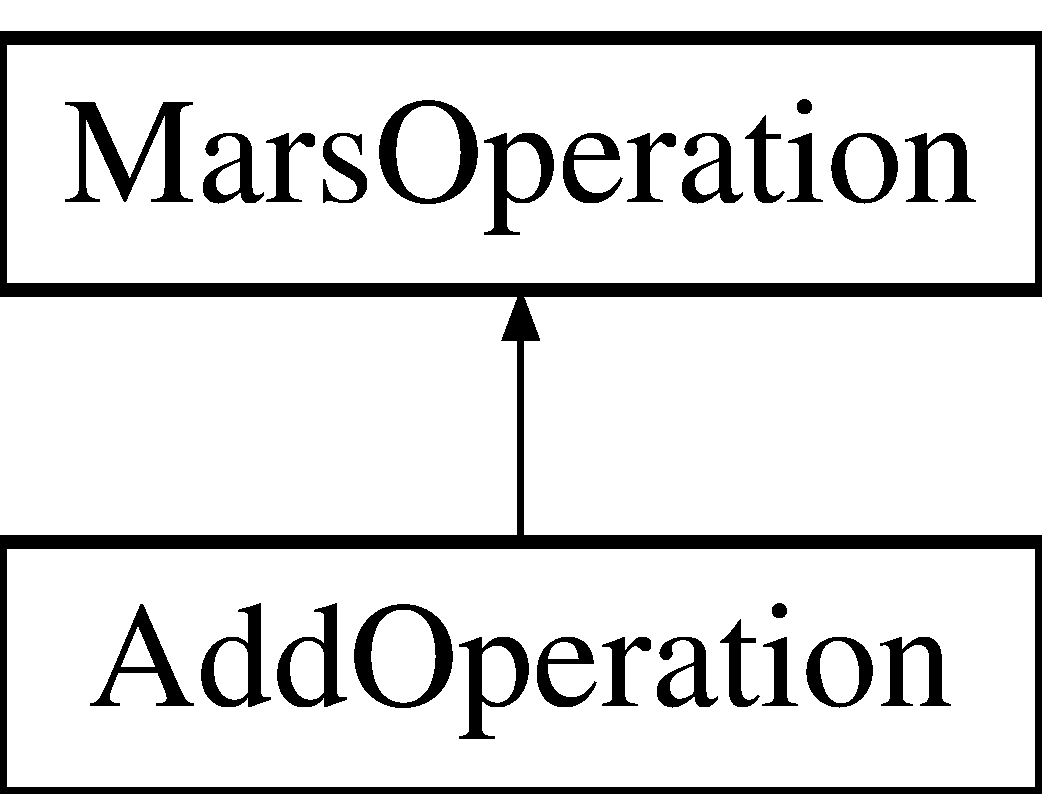
\includegraphics[height=2.000000cm]{classAddOperation}
\end{center}
\end{figure}
\subsection*{Public Member Functions}
\begin{DoxyCompactItemize}
\item 
\mbox{\Hypertarget{classAddOperation_a09f26b6d19ad82d86965f929f1a133ee}\label{classAddOperation_a09f26b6d19ad82d86965f929f1a133ee}} 
std\+::shared\+\_\+ptr$<$ \hyperlink{classProcessAction}{Process\+Action} $>$ {\bfseries run\+Operation} (\hyperlink{classOperationParamsInstructions}{Operation\+Params\+Instructions} $\ast$oper\+Params) override
\item 
\mbox{\Hypertarget{classAddOperation_a5a1373c509e314045ca2483019bd0739}\label{classAddOperation_a5a1373c509e314045ca2483019bd0739}} 
virtual std\+::shared\+\_\+ptr$<$ \hyperlink{classProcessAction}{Process\+Action} $>$ {\bfseries run\+Operation} (\hyperlink{classOperationParamsMixed}{Operation\+Params\+Mixed} $\ast$oper\+Params)
\end{DoxyCompactItemize}


\subsection{Detailed Description}
Class representing A\+DD operation 

The documentation for this class was generated from the following files\+:\begin{DoxyCompactItemize}
\item 
logic/mars/Add\+Operation.\+h\item 
logic/mars/Add\+Operation.\+cpp\end{DoxyCompactItemize}

\hypertarget{classCatch_1_1Detail_1_1Approx}{}\section{Catch\+:\+:Detail\+:\+:Approx Class Reference}
\label{classCatch_1_1Detail_1_1Approx}\index{Catch\+::\+Detail\+::\+Approx@{Catch\+::\+Detail\+::\+Approx}}
\subsection*{Public Member Functions}
\begin{DoxyCompactItemize}
\item 
\mbox{\Hypertarget{classCatch_1_1Detail_1_1Approx_a1a8618ea8db08c66bd3d9fe8f74b957a}\label{classCatch_1_1Detail_1_1Approx_a1a8618ea8db08c66bd3d9fe8f74b957a}} 
{\bfseries Approx} (double value)
\item 
\mbox{\Hypertarget{classCatch_1_1Detail_1_1Approx_a807330c63266fc914abdf6e461255a54}\label{classCatch_1_1Detail_1_1Approx_a807330c63266fc914abdf6e461255a54}} 
{\bfseries Approx} (\hyperlink{classCatch_1_1Detail_1_1Approx}{Approx} const \&other)
\item 
\mbox{\Hypertarget{classCatch_1_1Detail_1_1Approx_a48c9cbc28a05dc9dc8c3973b9eae2268}\label{classCatch_1_1Detail_1_1Approx_a48c9cbc28a05dc9dc8c3973b9eae2268}} 
\hyperlink{classCatch_1_1Detail_1_1Approx}{Approx} {\bfseries operator()} (double value)
\item 
\mbox{\Hypertarget{classCatch_1_1Detail_1_1Approx_a05c50c3ad0a971fab19345b5d94979a9}\label{classCatch_1_1Detail_1_1Approx_a05c50c3ad0a971fab19345b5d94979a9}} 
\hyperlink{classCatch_1_1Detail_1_1Approx}{Approx} \& {\bfseries epsilon} (double new\+Epsilon)
\item 
\mbox{\Hypertarget{classCatch_1_1Detail_1_1Approx_a82f7049b41c16e6234275641fad22218}\label{classCatch_1_1Detail_1_1Approx_a82f7049b41c16e6234275641fad22218}} 
\hyperlink{classCatch_1_1Detail_1_1Approx}{Approx} \& {\bfseries margin} (double new\+Margin)
\item 
\mbox{\Hypertarget{classCatch_1_1Detail_1_1Approx_acd80f0737bf38112beacd5ca95bef113}\label{classCatch_1_1Detail_1_1Approx_acd80f0737bf38112beacd5ca95bef113}} 
\hyperlink{classCatch_1_1Detail_1_1Approx}{Approx} \& {\bfseries scale} (double new\+Scale)
\item 
\mbox{\Hypertarget{classCatch_1_1Detail_1_1Approx_a972fd9ac60607483263f1b0f0f9955e6}\label{classCatch_1_1Detail_1_1Approx_a972fd9ac60607483263f1b0f0f9955e6}} 
std\+::string {\bfseries to\+String} () const
\end{DoxyCompactItemize}
\subsection*{Static Public Member Functions}
\begin{DoxyCompactItemize}
\item 
\mbox{\Hypertarget{classCatch_1_1Detail_1_1Approx_aaf86dc0ee92272ac2d9839197a07951d}\label{classCatch_1_1Detail_1_1Approx_aaf86dc0ee92272ac2d9839197a07951d}} 
static \hyperlink{classCatch_1_1Detail_1_1Approx}{Approx} {\bfseries custom} ()
\end{DoxyCompactItemize}
\subsection*{Friends}
\begin{DoxyCompactItemize}
\item 
\mbox{\Hypertarget{classCatch_1_1Detail_1_1Approx_ac766f044f1c63f0c5997982baefd9049}\label{classCatch_1_1Detail_1_1Approx_ac766f044f1c63f0c5997982baefd9049}} 
bool {\bfseries operator==} (double lhs, \hyperlink{classCatch_1_1Detail_1_1Approx}{Approx} const \&rhs)
\item 
\mbox{\Hypertarget{classCatch_1_1Detail_1_1Approx_a35999631e6cef569f9da9f3fa910db22}\label{classCatch_1_1Detail_1_1Approx_a35999631e6cef569f9da9f3fa910db22}} 
bool {\bfseries operator==} (\hyperlink{classCatch_1_1Detail_1_1Approx}{Approx} const \&lhs, double rhs)
\item 
\mbox{\Hypertarget{classCatch_1_1Detail_1_1Approx_a83b3763569a7ecc143c335b630be0e47}\label{classCatch_1_1Detail_1_1Approx_a83b3763569a7ecc143c335b630be0e47}} 
bool {\bfseries operator!=} (double lhs, \hyperlink{classCatch_1_1Detail_1_1Approx}{Approx} const \&rhs)
\item 
\mbox{\Hypertarget{classCatch_1_1Detail_1_1Approx_a7497ef839f8026cc0edd6269a80f3e09}\label{classCatch_1_1Detail_1_1Approx_a7497ef839f8026cc0edd6269a80f3e09}} 
bool {\bfseries operator!=} (\hyperlink{classCatch_1_1Detail_1_1Approx}{Approx} const \&lhs, double rhs)
\item 
\mbox{\Hypertarget{classCatch_1_1Detail_1_1Approx_aa2bfad80c8c138eac1f0b56910a7d3f2}\label{classCatch_1_1Detail_1_1Approx_aa2bfad80c8c138eac1f0b56910a7d3f2}} 
bool {\bfseries operator$<$=} (double lhs, \hyperlink{classCatch_1_1Detail_1_1Approx}{Approx} const \&rhs)
\item 
\mbox{\Hypertarget{classCatch_1_1Detail_1_1Approx_a75c9382b61421ffab3559c3506182d8f}\label{classCatch_1_1Detail_1_1Approx_a75c9382b61421ffab3559c3506182d8f}} 
bool {\bfseries operator$<$=} (\hyperlink{classCatch_1_1Detail_1_1Approx}{Approx} const \&lhs, double rhs)
\item 
\mbox{\Hypertarget{classCatch_1_1Detail_1_1Approx_a4e60095c615a0e6bdd6e8663cd24090b}\label{classCatch_1_1Detail_1_1Approx_a4e60095c615a0e6bdd6e8663cd24090b}} 
bool {\bfseries operator$>$=} (double lhs, \hyperlink{classCatch_1_1Detail_1_1Approx}{Approx} const \&rhs)
\item 
\mbox{\Hypertarget{classCatch_1_1Detail_1_1Approx_adaba11ee9aabb4d51d4855f09aa7f7df}\label{classCatch_1_1Detail_1_1Approx_adaba11ee9aabb4d51d4855f09aa7f7df}} 
bool {\bfseries operator$>$=} (\hyperlink{classCatch_1_1Detail_1_1Approx}{Approx} const \&lhs, double rhs)
\end{DoxyCompactItemize}


The documentation for this class was generated from the following file\+:\begin{DoxyCompactItemize}
\item 
test\+\_\+cases/catch.\+hpp\end{DoxyCompactItemize}

\hypertarget{structCatch_1_1AssertionInfo}{}\section{Catch\+:\+:Assertion\+Info Struct Reference}
\label{structCatch_1_1AssertionInfo}\index{Catch\+::\+Assertion\+Info@{Catch\+::\+Assertion\+Info}}
\subsection*{Public Member Functions}
\begin{DoxyCompactItemize}
\item 
\mbox{\Hypertarget{structCatch_1_1AssertionInfo_aaf6cc3eebd40391e54d37ed42953c73f}\label{structCatch_1_1AssertionInfo_aaf6cc3eebd40391e54d37ed42953c73f}} 
{\bfseries Assertion\+Info} (std\+::string const \&\+\_\+macro\+Name, \hyperlink{structCatch_1_1SourceLineInfo}{Source\+Line\+Info} const \&\+\_\+line\+Info, std\+::string const \&\+\_\+captured\+Expression, Result\+Disposition\+::\+Flags \+\_\+result\+Disposition)
\end{DoxyCompactItemize}
\subsection*{Public Attributes}
\begin{DoxyCompactItemize}
\item 
\mbox{\Hypertarget{structCatch_1_1AssertionInfo_ac2e59e8c89e00eb3390768f50d540b18}\label{structCatch_1_1AssertionInfo_ac2e59e8c89e00eb3390768f50d540b18}} 
std\+::string {\bfseries macro\+Name}
\item 
\mbox{\Hypertarget{structCatch_1_1AssertionInfo_a17bdbb404ba12658034f833be2f4c3e7}\label{structCatch_1_1AssertionInfo_a17bdbb404ba12658034f833be2f4c3e7}} 
\hyperlink{structCatch_1_1SourceLineInfo}{Source\+Line\+Info} {\bfseries line\+Info}
\item 
\mbox{\Hypertarget{structCatch_1_1AssertionInfo_af7c1d3cbfa346e9a303030fa0ef0cb54}\label{structCatch_1_1AssertionInfo_af7c1d3cbfa346e9a303030fa0ef0cb54}} 
std\+::string {\bfseries captured\+Expression}
\item 
\mbox{\Hypertarget{structCatch_1_1AssertionInfo_a60353b3632ab2f827162f2b2d6911073}\label{structCatch_1_1AssertionInfo_a60353b3632ab2f827162f2b2d6911073}} 
Result\+Disposition\+::\+Flags {\bfseries result\+Disposition}
\end{DoxyCompactItemize}


The documentation for this struct was generated from the following file\+:\begin{DoxyCompactItemize}
\item 
test\+\_\+cases/catch.\+hpp\end{DoxyCompactItemize}

\hypertarget{classCatch_1_1AssertionResult}{}\section{Catch\+:\+:Assertion\+Result Class Reference}
\label{classCatch_1_1AssertionResult}\index{Catch\+::\+Assertion\+Result@{Catch\+::\+Assertion\+Result}}
\subsection*{Public Member Functions}
\begin{DoxyCompactItemize}
\item 
\mbox{\Hypertarget{classCatch_1_1AssertionResult_ab58aeec27052ba400633ed0e36cea692}\label{classCatch_1_1AssertionResult_ab58aeec27052ba400633ed0e36cea692}} 
{\bfseries Assertion\+Result} (\hyperlink{structCatch_1_1AssertionInfo}{Assertion\+Info} const \&info, \hyperlink{structCatch_1_1AssertionResultData}{Assertion\+Result\+Data} const \&data)
\item 
\mbox{\Hypertarget{classCatch_1_1AssertionResult_ae39658b71c4afc3c8a859043b0e97027}\label{classCatch_1_1AssertionResult_ae39658b71c4afc3c8a859043b0e97027}} 
bool {\bfseries is\+Ok} () const
\item 
\mbox{\Hypertarget{classCatch_1_1AssertionResult_ac5cc872b721d5fb65d87221d30b22fdd}\label{classCatch_1_1AssertionResult_ac5cc872b721d5fb65d87221d30b22fdd}} 
bool {\bfseries succeeded} () const
\item 
\mbox{\Hypertarget{classCatch_1_1AssertionResult_ac810750194e1722489d2fd16e8c6a4a8}\label{classCatch_1_1AssertionResult_ac810750194e1722489d2fd16e8c6a4a8}} 
Result\+Was\+::\+Of\+Type {\bfseries get\+Result\+Type} () const
\item 
\mbox{\Hypertarget{classCatch_1_1AssertionResult_aba37b4fef1015989df2136592958e984}\label{classCatch_1_1AssertionResult_aba37b4fef1015989df2136592958e984}} 
bool {\bfseries has\+Expression} () const
\item 
\mbox{\Hypertarget{classCatch_1_1AssertionResult_aae37064b401919fa8ac480ef86cca924}\label{classCatch_1_1AssertionResult_aae37064b401919fa8ac480ef86cca924}} 
bool {\bfseries has\+Message} () const
\item 
\mbox{\Hypertarget{classCatch_1_1AssertionResult_a26a777f3959353c729544cb2ace0d279}\label{classCatch_1_1AssertionResult_a26a777f3959353c729544cb2ace0d279}} 
std\+::string {\bfseries get\+Expression} () const
\item 
\mbox{\Hypertarget{classCatch_1_1AssertionResult_aac35a0ca42d33bff6467c76573730f5e}\label{classCatch_1_1AssertionResult_aac35a0ca42d33bff6467c76573730f5e}} 
std\+::string {\bfseries get\+Expression\+In\+Macro} () const
\item 
\mbox{\Hypertarget{classCatch_1_1AssertionResult_a78c43506c2b3d8cc1fb141a97d09ec94}\label{classCatch_1_1AssertionResult_a78c43506c2b3d8cc1fb141a97d09ec94}} 
bool {\bfseries has\+Expanded\+Expression} () const
\item 
\mbox{\Hypertarget{classCatch_1_1AssertionResult_aaa46070791a6c07caaed86229b8d9d75}\label{classCatch_1_1AssertionResult_aaa46070791a6c07caaed86229b8d9d75}} 
std\+::string {\bfseries get\+Expanded\+Expression} () const
\item 
\mbox{\Hypertarget{classCatch_1_1AssertionResult_ae730943beed46921b09383c673e35786}\label{classCatch_1_1AssertionResult_ae730943beed46921b09383c673e35786}} 
std\+::string {\bfseries get\+Message} () const
\item 
\mbox{\Hypertarget{classCatch_1_1AssertionResult_aa4d3fdbfe276a69a035762dbb790800f}\label{classCatch_1_1AssertionResult_aa4d3fdbfe276a69a035762dbb790800f}} 
\hyperlink{structCatch_1_1SourceLineInfo}{Source\+Line\+Info} {\bfseries get\+Source\+Info} () const
\item 
\mbox{\Hypertarget{classCatch_1_1AssertionResult_aaefd9a0384282fd08a4a72aa19bd0628}\label{classCatch_1_1AssertionResult_aaefd9a0384282fd08a4a72aa19bd0628}} 
std\+::string {\bfseries get\+Test\+Macro\+Name} () const
\item 
\mbox{\Hypertarget{classCatch_1_1AssertionResult_a406884d8b8209c80078706724c528df5}\label{classCatch_1_1AssertionResult_a406884d8b8209c80078706724c528df5}} 
void {\bfseries discard\+Decomposed\+Expression} () const
\item 
\mbox{\Hypertarget{classCatch_1_1AssertionResult_ac0b1d268a3ffa1f1fb305cad9435d824}\label{classCatch_1_1AssertionResult_ac0b1d268a3ffa1f1fb305cad9435d824}} 
void {\bfseries expand\+Decomposed\+Expression} () const
\end{DoxyCompactItemize}
\subsection*{Protected Attributes}
\begin{DoxyCompactItemize}
\item 
\mbox{\Hypertarget{classCatch_1_1AssertionResult_a3e7236f73a51d6fc8bb9dfdefcee7772}\label{classCatch_1_1AssertionResult_a3e7236f73a51d6fc8bb9dfdefcee7772}} 
\hyperlink{structCatch_1_1AssertionInfo}{Assertion\+Info} {\bfseries m\+\_\+info}
\item 
\mbox{\Hypertarget{classCatch_1_1AssertionResult_add3455b8bbedb0d643e18da67c66b4f7}\label{classCatch_1_1AssertionResult_add3455b8bbedb0d643e18da67c66b4f7}} 
\hyperlink{structCatch_1_1AssertionResultData}{Assertion\+Result\+Data} {\bfseries m\+\_\+result\+Data}
\end{DoxyCompactItemize}


The documentation for this class was generated from the following file\+:\begin{DoxyCompactItemize}
\item 
test\+\_\+cases/catch.\+hpp\end{DoxyCompactItemize}

\hypertarget{structCatch_1_1AssertionResultData}{}\section{Catch\+:\+:Assertion\+Result\+Data Struct Reference}
\label{structCatch_1_1AssertionResultData}\index{Catch\+::\+Assertion\+Result\+Data@{Catch\+::\+Assertion\+Result\+Data}}
\subsection*{Public Member Functions}
\begin{DoxyCompactItemize}
\item 
\mbox{\Hypertarget{structCatch_1_1AssertionResultData_a3b4df7cd1f8228ea1144b5cd0af6006a}\label{structCatch_1_1AssertionResultData_a3b4df7cd1f8228ea1144b5cd0af6006a}} 
void {\bfseries negate} (bool parenthesize)
\item 
\mbox{\Hypertarget{structCatch_1_1AssertionResultData_adbc0629083cd2e76c3a78696453443b0}\label{structCatch_1_1AssertionResultData_adbc0629083cd2e76c3a78696453443b0}} 
std\+::string const  \& {\bfseries reconstruct\+Expression} () const
\end{DoxyCompactItemize}
\subsection*{Public Attributes}
\begin{DoxyCompactItemize}
\item 
\mbox{\Hypertarget{structCatch_1_1AssertionResultData_a45b2bf2ed11da83d09dd78a2b7a44cd4}\label{structCatch_1_1AssertionResultData_a45b2bf2ed11da83d09dd78a2b7a44cd4}} 
\hyperlink{structCatch_1_1DecomposedExpression}{Decomposed\+Expression} const  $\ast$ {\bfseries decomposed\+Expression}
\item 
\mbox{\Hypertarget{structCatch_1_1AssertionResultData_a9e809d36fffbeb1c7d0cbe7382dd9595}\label{structCatch_1_1AssertionResultData_a9e809d36fffbeb1c7d0cbe7382dd9595}} 
std\+::string {\bfseries reconstructed\+Expression}
\item 
\mbox{\Hypertarget{structCatch_1_1AssertionResultData_ac34215803c4c4a88f795879f61c1f7b4}\label{structCatch_1_1AssertionResultData_ac34215803c4c4a88f795879f61c1f7b4}} 
std\+::string {\bfseries message}
\item 
\mbox{\Hypertarget{structCatch_1_1AssertionResultData_a7ceab4a7ff722aec5587e3748caf66b7}\label{structCatch_1_1AssertionResultData_a7ceab4a7ff722aec5587e3748caf66b7}} 
Result\+Was\+::\+Of\+Type {\bfseries result\+Type}
\item 
\mbox{\Hypertarget{structCatch_1_1AssertionResultData_a17773c6f999cfded12e470b0321694a1}\label{structCatch_1_1AssertionResultData_a17773c6f999cfded12e470b0321694a1}} 
bool {\bfseries negated}
\item 
\mbox{\Hypertarget{structCatch_1_1AssertionResultData_a8418e3744b5486cb7f0d79c84569078e}\label{structCatch_1_1AssertionResultData_a8418e3744b5486cb7f0d79c84569078e}} 
bool {\bfseries parenthesized}
\end{DoxyCompactItemize}


The documentation for this struct was generated from the following file\+:\begin{DoxyCompactItemize}
\item 
test\+\_\+cases/catch.\+hpp\end{DoxyCompactItemize}

\hypertarget{structCatch_1_1AutoReg}{}\section{Catch\+:\+:Auto\+Reg Struct Reference}
\label{structCatch_1_1AutoReg}\index{Catch\+::\+Auto\+Reg@{Catch\+::\+Auto\+Reg}}
\subsection*{Public Member Functions}
\begin{DoxyCompactItemize}
\item 
\mbox{\Hypertarget{structCatch_1_1AutoReg_af224f4568d57b8652474df475a164a8c}\label{structCatch_1_1AutoReg_af224f4568d57b8652474df475a164a8c}} 
{\bfseries Auto\+Reg} (Test\+Function function, \hyperlink{structCatch_1_1SourceLineInfo}{Source\+Line\+Info} const \&line\+Info, \hyperlink{structCatch_1_1NameAndDesc}{Name\+And\+Desc} const \&name\+And\+Desc)
\item 
\mbox{\Hypertarget{structCatch_1_1AutoReg_a1bf9207fe0a02b46dc0ab1cc03cbe738}\label{structCatch_1_1AutoReg_a1bf9207fe0a02b46dc0ab1cc03cbe738}} 
{\footnotesize template$<$typename C $>$ }\\{\bfseries Auto\+Reg} (void(C\+::$\ast$method)(), char const $\ast$class\+Name, \hyperlink{structCatch_1_1NameAndDesc}{Name\+And\+Desc} const \&name\+And\+Desc, \hyperlink{structCatch_1_1SourceLineInfo}{Source\+Line\+Info} const \&line\+Info)
\end{DoxyCompactItemize}


The documentation for this struct was generated from the following file\+:\begin{DoxyCompactItemize}
\item 
test\+\_\+cases/catch.\+hpp\end{DoxyCompactItemize}

\hypertarget{classCatch_1_1BetweenGenerator}{}\section{Catch\+:\+:Between\+Generator$<$ T $>$ Class Template Reference}
\label{classCatch_1_1BetweenGenerator}\index{Catch\+::\+Between\+Generator$<$ T $>$@{Catch\+::\+Between\+Generator$<$ T $>$}}
Inheritance diagram for Catch\+:\+:Between\+Generator$<$ T $>$\+:\begin{figure}[H]
\begin{center}
\leavevmode
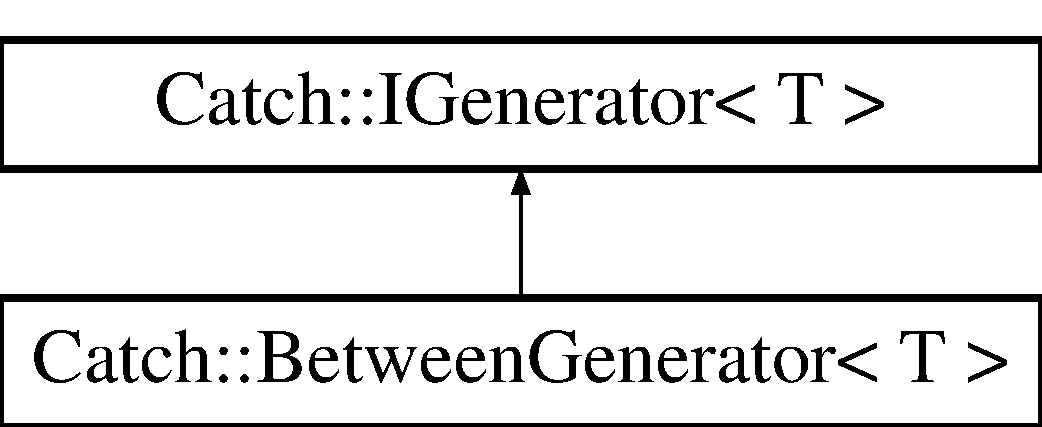
\includegraphics[height=2.000000cm]{classCatch_1_1BetweenGenerator}
\end{center}
\end{figure}
\subsection*{Public Member Functions}
\begin{DoxyCompactItemize}
\item 
\mbox{\Hypertarget{classCatch_1_1BetweenGenerator_a835a057d691ae37caef660624099b51c}\label{classCatch_1_1BetweenGenerator_a835a057d691ae37caef660624099b51c}} 
{\bfseries Between\+Generator} (T from, T to)
\item 
\mbox{\Hypertarget{classCatch_1_1BetweenGenerator_a913f74bb0c23b3bc0127abfffdabbd94}\label{classCatch_1_1BetweenGenerator_a913f74bb0c23b3bc0127abfffdabbd94}} 
virtual T {\bfseries get\+Value} (std\+::size\+\_\+t index) const
\item 
\mbox{\Hypertarget{classCatch_1_1BetweenGenerator_af65a1fe51f9b1106fc676e3dd189adb6}\label{classCatch_1_1BetweenGenerator_af65a1fe51f9b1106fc676e3dd189adb6}} 
virtual std\+::size\+\_\+t {\bfseries size} () const
\end{DoxyCompactItemize}


The documentation for this class was generated from the following file\+:\begin{DoxyCompactItemize}
\item 
test\+\_\+cases/catch.\+hpp\end{DoxyCompactItemize}

\hypertarget{classCatch_1_1BinaryExpression}{}\section{Catch\+:\+:Binary\+Expression$<$ LhsT, Op, RhsT $>$ Class Template Reference}
\label{classCatch_1_1BinaryExpression}\index{Catch\+::\+Binary\+Expression$<$ Lhs\+T, Op, Rhs\+T $>$@{Catch\+::\+Binary\+Expression$<$ Lhs\+T, Op, Rhs\+T $>$}}
Inheritance diagram for Catch\+:\+:Binary\+Expression$<$ LhsT, Op, RhsT $>$\+:\begin{figure}[H]
\begin{center}
\leavevmode
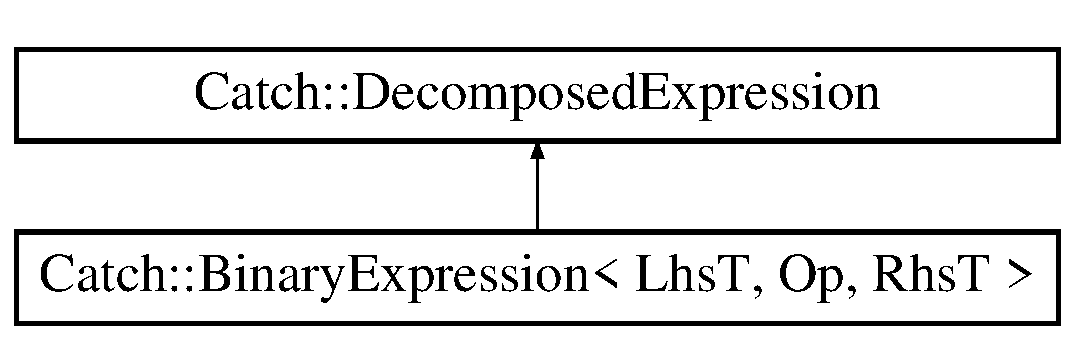
\includegraphics[height=2.000000cm]{classCatch_1_1BinaryExpression}
\end{center}
\end{figure}
\subsection*{Public Member Functions}
\begin{DoxyCompactItemize}
\item 
\mbox{\Hypertarget{classCatch_1_1BinaryExpression_a0d81384761aba5f7a6d5f4fc7e7944f3}\label{classCatch_1_1BinaryExpression_a0d81384761aba5f7a6d5f4fc7e7944f3}} 
{\bfseries Binary\+Expression} (\hyperlink{classCatch_1_1ResultBuilder}{Result\+Builder} \&rb, LhsT lhs, RhsT rhs)
\item 
\mbox{\Hypertarget{classCatch_1_1BinaryExpression_a2147a858eb5866e5643d0ef321064aa1}\label{classCatch_1_1BinaryExpression_a2147a858eb5866e5643d0ef321064aa1}} 
\hyperlink{classCatch_1_1BinaryExpression}{Binary\+Expression} \& {\bfseries operator=} (\hyperlink{classCatch_1_1BinaryExpression}{Binary\+Expression} \&)
\item 
\mbox{\Hypertarget{classCatch_1_1BinaryExpression_aa1dba7f316f70902859b8eab27692dfb}\label{classCatch_1_1BinaryExpression_aa1dba7f316f70902859b8eab27692dfb}} 
void {\bfseries end\+Expression} () const
\item 
\mbox{\Hypertarget{classCatch_1_1BinaryExpression_a4c617c0b6a73a9cafbbf900909c7c258}\label{classCatch_1_1BinaryExpression_a4c617c0b6a73a9cafbbf900909c7c258}} 
virtual bool {\bfseries is\+Binary\+Expression} () const C\+A\+T\+C\+H\+\_\+\+O\+V\+E\+R\+R\+I\+DE
\item 
\mbox{\Hypertarget{classCatch_1_1BinaryExpression_a6ed73ff9af9c229f9fa3d35d019f9e37}\label{classCatch_1_1BinaryExpression_a6ed73ff9af9c229f9fa3d35d019f9e37}} 
virtual void {\bfseries reconstruct\+Expression} (std\+::string \&dest) const C\+A\+T\+C\+H\+\_\+\+O\+V\+E\+R\+R\+I\+DE
\end{DoxyCompactItemize}


The documentation for this class was generated from the following file\+:\begin{DoxyCompactItemize}
\item 
test\+\_\+cases/catch.\+hpp\end{DoxyCompactItemize}

\hypertarget{structCatch_1_1Detail_1_1BorgType}{}\section{Catch\+:\+:Detail\+:\+:Borg\+Type Struct Reference}
\label{structCatch_1_1Detail_1_1BorgType}\index{Catch\+::\+Detail\+::\+Borg\+Type@{Catch\+::\+Detail\+::\+Borg\+Type}}
\subsection*{Public Member Functions}
\begin{DoxyCompactItemize}
\item 
\mbox{\Hypertarget{structCatch_1_1Detail_1_1BorgType_a780a9946ed0d654f0bfc043c8fc505d8}\label{structCatch_1_1Detail_1_1BorgType_a780a9946ed0d654f0bfc043c8fc505d8}} 
{\footnotesize template$<$typename T $>$ }\\{\bfseries Borg\+Type} (T const \&)
\end{DoxyCompactItemize}


The documentation for this struct was generated from the following file\+:\begin{DoxyCompactItemize}
\item 
test\+\_\+cases/catch.\+hpp\end{DoxyCompactItemize}

\hypertarget{structCatch_1_1Matchers_1_1StdString_1_1CasedString}{}\section{Catch\+:\+:Matchers\+:\+:Std\+String\+:\+:Cased\+String Struct Reference}
\label{structCatch_1_1Matchers_1_1StdString_1_1CasedString}\index{Catch\+::\+Matchers\+::\+Std\+String\+::\+Cased\+String@{Catch\+::\+Matchers\+::\+Std\+String\+::\+Cased\+String}}
\subsection*{Public Member Functions}
\begin{DoxyCompactItemize}
\item 
\mbox{\Hypertarget{structCatch_1_1Matchers_1_1StdString_1_1CasedString_aa88bbc5acd2bff22351d8d4b1816b561}\label{structCatch_1_1Matchers_1_1StdString_1_1CasedString_aa88bbc5acd2bff22351d8d4b1816b561}} 
{\bfseries Cased\+String} (std\+::string const \&str, Case\+Sensitive\+::\+Choice case\+Sensitivity)
\item 
\mbox{\Hypertarget{structCatch_1_1Matchers_1_1StdString_1_1CasedString_a77639b1165c01f424ee0e96f53335010}\label{structCatch_1_1Matchers_1_1StdString_1_1CasedString_a77639b1165c01f424ee0e96f53335010}} 
std\+::string {\bfseries adjust\+String} (std\+::string const \&str) const
\item 
\mbox{\Hypertarget{structCatch_1_1Matchers_1_1StdString_1_1CasedString_a9759155344d696b2476d764a1d95fcc9}\label{structCatch_1_1Matchers_1_1StdString_1_1CasedString_a9759155344d696b2476d764a1d95fcc9}} 
std\+::string {\bfseries case\+Sensitivity\+Suffix} () const
\end{DoxyCompactItemize}
\subsection*{Public Attributes}
\begin{DoxyCompactItemize}
\item 
\mbox{\Hypertarget{structCatch_1_1Matchers_1_1StdString_1_1CasedString_ae1c2864c986941536a6e94cca0528f92}\label{structCatch_1_1Matchers_1_1StdString_1_1CasedString_ae1c2864c986941536a6e94cca0528f92}} 
Case\+Sensitive\+::\+Choice {\bfseries m\+\_\+case\+Sensitivity}
\item 
\mbox{\Hypertarget{structCatch_1_1Matchers_1_1StdString_1_1CasedString_ad05dbc99aba3c3c386d6b856b213f911}\label{structCatch_1_1Matchers_1_1StdString_1_1CasedString_ad05dbc99aba3c3c386d6b856b213f911}} 
std\+::string {\bfseries m\+\_\+str}
\end{DoxyCompactItemize}


The documentation for this struct was generated from the following file\+:\begin{DoxyCompactItemize}
\item 
test\+\_\+cases/catch.\+hpp\end{DoxyCompactItemize}

\hypertarget{structCatch_1_1CaseSensitive}{}\section{Catch\+:\+:Case\+Sensitive Struct Reference}
\label{structCatch_1_1CaseSensitive}\index{Catch\+::\+Case\+Sensitive@{Catch\+::\+Case\+Sensitive}}
\subsection*{Public Types}
\begin{DoxyCompactItemize}
\item 
\mbox{\Hypertarget{structCatch_1_1CaseSensitive_aad49d3aee2d97066642fffa919685c6a}\label{structCatch_1_1CaseSensitive_aad49d3aee2d97066642fffa919685c6a}} 
enum {\bfseries Choice} \{ {\bfseries Yes}, 
{\bfseries No}
 \}
\end{DoxyCompactItemize}


The documentation for this struct was generated from the following file\+:\begin{DoxyCompactItemize}
\item 
test\+\_\+cases/catch.\+hpp\end{DoxyCompactItemize}

\hypertarget{classMARS_1_1Code}{}\section{M\+A\+RS\+:\+:Code Class Reference}
\label{classMARS_1_1Code}\index{M\+A\+R\+S\+::\+Code@{M\+A\+R\+S\+::\+Code}}
Inheritance diagram for M\+A\+RS\+:\+:Code\+:\begin{figure}[H]
\begin{center}
\leavevmode
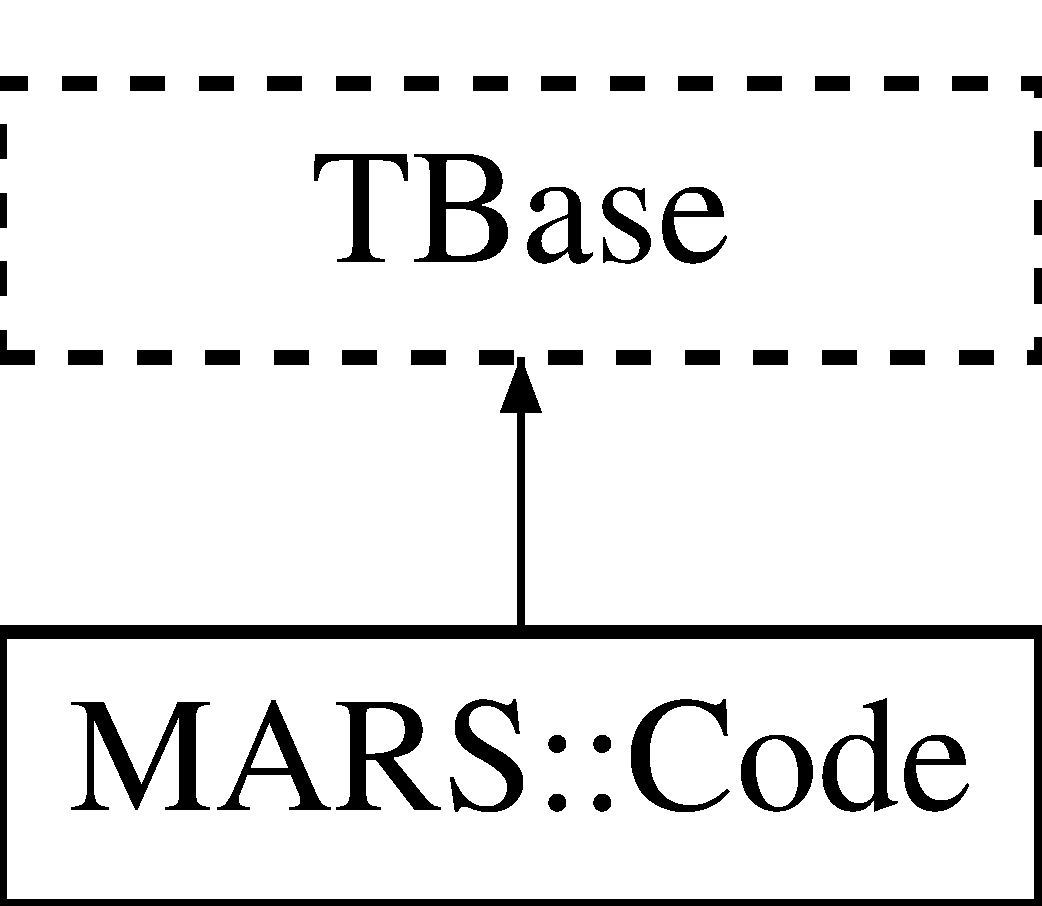
\includegraphics[height=2.000000cm]{classMARS_1_1Code}
\end{center}
\end{figure}
\subsection*{Public Member Functions}
\begin{DoxyCompactItemize}
\item 
\mbox{\Hypertarget{classMARS_1_1Code_a0da16d905b467bce02e3d12afc28941a}\label{classMARS_1_1Code_a0da16d905b467bce02e3d12afc28941a}} 
{\bfseries Code} (const \hyperlink{classMARS_1_1Code}{Code} \&)
\item 
\mbox{\Hypertarget{classMARS_1_1Code_a804ba40d197d943f8763ae34a138e66c}\label{classMARS_1_1Code_a804ba40d197d943f8763ae34a138e66c}} 
\hyperlink{classMARS_1_1Code}{Code} \& {\bfseries operator=} (const \hyperlink{classMARS_1_1Code}{Code} \&)
\item 
\mbox{\Hypertarget{classMARS_1_1Code_a105c1d70af553f2115446fbdf5ea8eb8}\label{classMARS_1_1Code_a105c1d70af553f2115446fbdf5ea8eb8}} 
void {\bfseries \+\_\+\+\_\+set\+\_\+code} (const std\+::string \&val)
\item 
\mbox{\Hypertarget{classMARS_1_1Code_a454b144403c876a6256c54e6042b5b37}\label{classMARS_1_1Code_a454b144403c876a6256c54e6042b5b37}} 
bool {\bfseries operator==} (const \hyperlink{classMARS_1_1Code}{Code} \&rhs) const
\item 
\mbox{\Hypertarget{classMARS_1_1Code_aee6111f0a913c527b24029e70233a44a}\label{classMARS_1_1Code_aee6111f0a913c527b24029e70233a44a}} 
bool {\bfseries operator!=} (const \hyperlink{classMARS_1_1Code}{Code} \&rhs) const
\item 
\mbox{\Hypertarget{classMARS_1_1Code_a528ce64bcde9095dda3d06309361bef4}\label{classMARS_1_1Code_a528ce64bcde9095dda3d06309361bef4}} 
bool {\bfseries operator$<$} (const \hyperlink{classMARS_1_1Code}{Code} \&) const
\item 
\mbox{\Hypertarget{classMARS_1_1Code_a9b78ec36f0e776506be23820c63021a8}\label{classMARS_1_1Code_a9b78ec36f0e776506be23820c63021a8}} 
uint32\+\_\+t {\bfseries read} (\+::apache\+::thrift\+::protocol\+::\+T\+Protocol $\ast$iprot)
\item 
\mbox{\Hypertarget{classMARS_1_1Code_a7729a8fdfae083d3dd74e9088b41a975}\label{classMARS_1_1Code_a7729a8fdfae083d3dd74e9088b41a975}} 
uint32\+\_\+t {\bfseries write} (\+::apache\+::thrift\+::protocol\+::\+T\+Protocol $\ast$oprot) const
\item 
\mbox{\Hypertarget{classMARS_1_1Code_ae3f0dd85af90fb7162a2e73e9a6ea3e2}\label{classMARS_1_1Code_ae3f0dd85af90fb7162a2e73e9a6ea3e2}} 
virtual void {\bfseries print\+To} (std\+::ostream \&out) const
\end{DoxyCompactItemize}
\subsection*{Public Attributes}
\begin{DoxyCompactItemize}
\item 
\mbox{\Hypertarget{classMARS_1_1Code_a29ea96edab2f02e49a96b47c1989ad7d}\label{classMARS_1_1Code_a29ea96edab2f02e49a96b47c1989ad7d}} 
std\+::string {\bfseries code}
\item 
\mbox{\Hypertarget{classMARS_1_1Code_ac52cfc9f20d2e1d2a2942183083f1b4e}\label{classMARS_1_1Code_ac52cfc9f20d2e1d2a2942183083f1b4e}} 
\hyperlink{structMARS_1_1__Code____isset}{\+\_\+\+Code\+\_\+\+\_\+isset} {\bfseries \+\_\+\+\_\+isset}
\end{DoxyCompactItemize}


The documentation for this class was generated from the following files\+:\begin{DoxyCompactItemize}
\item 
gen-\/cpp/mars\+\_\+types.\+h\item 
gen-\/cpp/mars\+\_\+types.\+cpp\end{DoxyCompactItemize}

\hypertarget{classCatch_1_1CompositeGenerator}{}\section{Catch\+:\+:Composite\+Generator$<$ T $>$ Class Template Reference}
\label{classCatch_1_1CompositeGenerator}\index{Catch\+::\+Composite\+Generator$<$ T $>$@{Catch\+::\+Composite\+Generator$<$ T $>$}}
\subsection*{Public Member Functions}
\begin{DoxyCompactItemize}
\item 
\mbox{\Hypertarget{classCatch_1_1CompositeGenerator_a21a7070a00e4a6fe021294c356692692}\label{classCatch_1_1CompositeGenerator_a21a7070a00e4a6fe021294c356692692}} 
{\bfseries Composite\+Generator} (\hyperlink{classCatch_1_1CompositeGenerator}{Composite\+Generator} \&other)
\item 
\mbox{\Hypertarget{classCatch_1_1CompositeGenerator_ac3c57cf4ca5472f440bf71e2936bcd4a}\label{classCatch_1_1CompositeGenerator_ac3c57cf4ca5472f440bf71e2936bcd4a}} 
\hyperlink{classCatch_1_1CompositeGenerator}{Composite\+Generator} \& {\bfseries set\+File\+Info} (const char $\ast$file\+Info)
\item 
\mbox{\Hypertarget{classCatch_1_1CompositeGenerator_a83d6c941e2e735b9528e6e832f7b76e7}\label{classCatch_1_1CompositeGenerator_a83d6c941e2e735b9528e6e832f7b76e7}} 
{\bfseries operator T} () const
\item 
\mbox{\Hypertarget{classCatch_1_1CompositeGenerator_af3774d42ad2d3453d089ca599efe0517}\label{classCatch_1_1CompositeGenerator_af3774d42ad2d3453d089ca599efe0517}} 
void {\bfseries add} (const \hyperlink{structCatch_1_1IGenerator}{I\+Generator}$<$ T $>$ $\ast$generator)
\item 
\mbox{\Hypertarget{classCatch_1_1CompositeGenerator_a2e03f42df85cdd238aabd77a80b075d5}\label{classCatch_1_1CompositeGenerator_a2e03f42df85cdd238aabd77a80b075d5}} 
\hyperlink{classCatch_1_1CompositeGenerator}{Composite\+Generator} \& {\bfseries then} (\hyperlink{classCatch_1_1CompositeGenerator}{Composite\+Generator} \&other)
\item 
\mbox{\Hypertarget{classCatch_1_1CompositeGenerator_aefdc11bcfccdf07d2db5f0da3ed8758c}\label{classCatch_1_1CompositeGenerator_aefdc11bcfccdf07d2db5f0da3ed8758c}} 
\hyperlink{classCatch_1_1CompositeGenerator}{Composite\+Generator} \& {\bfseries then} (T value)
\end{DoxyCompactItemize}


The documentation for this class was generated from the following file\+:\begin{DoxyCompactItemize}
\item 
test\+\_\+cases/catch.\+hpp\end{DoxyCompactItemize}

\hypertarget{structCatch_1_1Matchers_1_1Vector_1_1ContainsElementMatcher}{}\section{Catch\+:\+:Matchers\+:\+:Vector\+:\+:Contains\+Element\+Matcher$<$ T $>$ Struct Template Reference}
\label{structCatch_1_1Matchers_1_1Vector_1_1ContainsElementMatcher}\index{Catch\+::\+Matchers\+::\+Vector\+::\+Contains\+Element\+Matcher$<$ T $>$@{Catch\+::\+Matchers\+::\+Vector\+::\+Contains\+Element\+Matcher$<$ T $>$}}
Inheritance diagram for Catch\+:\+:Matchers\+:\+:Vector\+:\+:Contains\+Element\+Matcher$<$ T $>$\+:\begin{figure}[H]
\begin{center}
\leavevmode
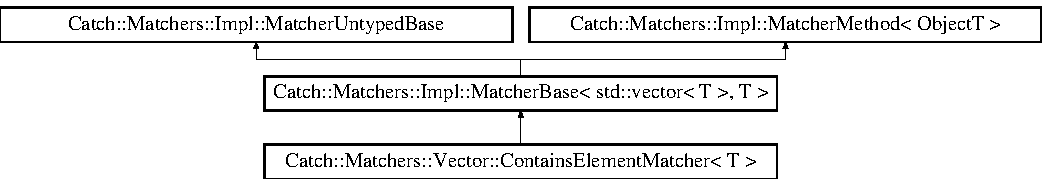
\includegraphics[height=2.400000cm]{structCatch_1_1Matchers_1_1Vector_1_1ContainsElementMatcher}
\end{center}
\end{figure}
\subsection*{Public Member Functions}
\begin{DoxyCompactItemize}
\item 
\mbox{\Hypertarget{structCatch_1_1Matchers_1_1Vector_1_1ContainsElementMatcher_a6a05740b5d3f89fac8de84ac0cff7b93}\label{structCatch_1_1Matchers_1_1Vector_1_1ContainsElementMatcher_a6a05740b5d3f89fac8de84ac0cff7b93}} 
{\bfseries Contains\+Element\+Matcher} (T const \&comparator)
\item 
\mbox{\Hypertarget{structCatch_1_1Matchers_1_1Vector_1_1ContainsElementMatcher_a95fd99879bcfbe129898bef922c92c17}\label{structCatch_1_1Matchers_1_1Vector_1_1ContainsElementMatcher_a95fd99879bcfbe129898bef922c92c17}} 
bool {\bfseries match} (std\+::vector$<$ T $>$ const \&v) const C\+A\+T\+C\+H\+\_\+\+O\+V\+E\+R\+R\+I\+DE
\item 
\mbox{\Hypertarget{structCatch_1_1Matchers_1_1Vector_1_1ContainsElementMatcher_a5a869772714dd045816707b74b217664}\label{structCatch_1_1Matchers_1_1Vector_1_1ContainsElementMatcher_a5a869772714dd045816707b74b217664}} 
virtual std\+::string {\bfseries describe} () const C\+A\+T\+C\+H\+\_\+\+O\+V\+E\+R\+R\+I\+DE
\end{DoxyCompactItemize}
\subsection*{Public Attributes}
\begin{DoxyCompactItemize}
\item 
\mbox{\Hypertarget{structCatch_1_1Matchers_1_1Vector_1_1ContainsElementMatcher_ab7eada6c4bbce1d21b44773262f9cb23}\label{structCatch_1_1Matchers_1_1Vector_1_1ContainsElementMatcher_ab7eada6c4bbce1d21b44773262f9cb23}} 
T const  \& {\bfseries m\+\_\+comparator}
\end{DoxyCompactItemize}
\subsection*{Additional Inherited Members}


The documentation for this struct was generated from the following file\+:\begin{DoxyCompactItemize}
\item 
test\+\_\+cases/catch.\+hpp\end{DoxyCompactItemize}

\hypertarget{structCatch_1_1Matchers_1_1StdString_1_1ContainsMatcher}{}\section{Catch\+:\+:Matchers\+:\+:Std\+String\+:\+:Contains\+Matcher Struct Reference}
\label{structCatch_1_1Matchers_1_1StdString_1_1ContainsMatcher}\index{Catch\+::\+Matchers\+::\+Std\+String\+::\+Contains\+Matcher@{Catch\+::\+Matchers\+::\+Std\+String\+::\+Contains\+Matcher}}
Inheritance diagram for Catch\+:\+:Matchers\+:\+:Std\+String\+:\+:Contains\+Matcher\+:\begin{figure}[H]
\begin{center}
\leavevmode
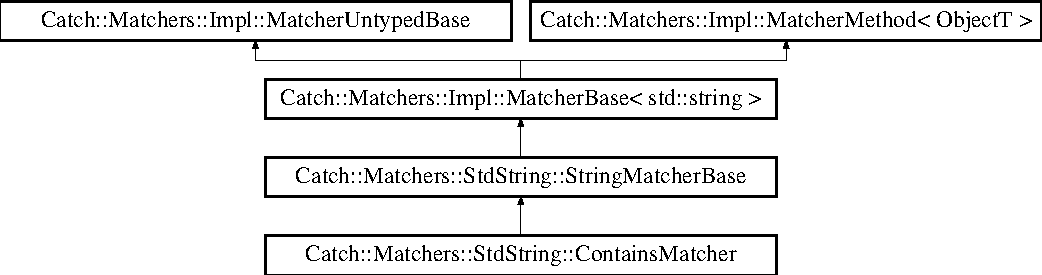
\includegraphics[height=3.696370cm]{structCatch_1_1Matchers_1_1StdString_1_1ContainsMatcher}
\end{center}
\end{figure}
\subsection*{Public Member Functions}
\begin{DoxyCompactItemize}
\item 
\mbox{\Hypertarget{structCatch_1_1Matchers_1_1StdString_1_1ContainsMatcher_acc892883c8409e34b28c9b39d4ef1fe3}\label{structCatch_1_1Matchers_1_1StdString_1_1ContainsMatcher_acc892883c8409e34b28c9b39d4ef1fe3}} 
{\bfseries Contains\+Matcher} (\hyperlink{structCatch_1_1Matchers_1_1StdString_1_1CasedString}{Cased\+String} const \&comparator)
\item 
\mbox{\Hypertarget{structCatch_1_1Matchers_1_1StdString_1_1ContainsMatcher_ae4d567347fa563e365f1044f29ab1042}\label{structCatch_1_1Matchers_1_1StdString_1_1ContainsMatcher_ae4d567347fa563e365f1044f29ab1042}} 
virtual bool {\bfseries match} (std\+::string const \&source) const C\+A\+T\+C\+H\+\_\+\+O\+V\+E\+R\+R\+I\+DE
\end{DoxyCompactItemize}
\subsection*{Additional Inherited Members}


The documentation for this struct was generated from the following file\+:\begin{DoxyCompactItemize}
\item 
test\+\_\+cases/catch.\+hpp\end{DoxyCompactItemize}

\hypertarget{structCatch_1_1Matchers_1_1Vector_1_1ContainsMatcher}{}\section{Catch\+:\+:Matchers\+:\+:Vector\+:\+:Contains\+Matcher$<$ T $>$ Struct Template Reference}
\label{structCatch_1_1Matchers_1_1Vector_1_1ContainsMatcher}\index{Catch\+::\+Matchers\+::\+Vector\+::\+Contains\+Matcher$<$ T $>$@{Catch\+::\+Matchers\+::\+Vector\+::\+Contains\+Matcher$<$ T $>$}}
Inheritance diagram for Catch\+:\+:Matchers\+:\+:Vector\+:\+:Contains\+Matcher$<$ T $>$\+:\begin{figure}[H]
\begin{center}
\leavevmode
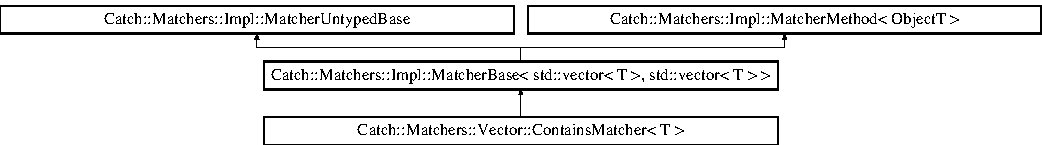
\includegraphics[height=1.944444cm]{structCatch_1_1Matchers_1_1Vector_1_1ContainsMatcher}
\end{center}
\end{figure}
\subsection*{Public Member Functions}
\begin{DoxyCompactItemize}
\item 
\mbox{\Hypertarget{structCatch_1_1Matchers_1_1Vector_1_1ContainsMatcher_ad8e92c8399be6dce75bb5702cdfab700}\label{structCatch_1_1Matchers_1_1Vector_1_1ContainsMatcher_ad8e92c8399be6dce75bb5702cdfab700}} 
{\bfseries Contains\+Matcher} (std\+::vector$<$ T $>$ const \&comparator)
\item 
\mbox{\Hypertarget{structCatch_1_1Matchers_1_1Vector_1_1ContainsMatcher_aba81516816a6796124dd4fe4843e7284}\label{structCatch_1_1Matchers_1_1Vector_1_1ContainsMatcher_aba81516816a6796124dd4fe4843e7284}} 
bool {\bfseries match} (std\+::vector$<$ T $>$ const \&v) const C\+A\+T\+C\+H\+\_\+\+O\+V\+E\+R\+R\+I\+DE
\item 
\mbox{\Hypertarget{structCatch_1_1Matchers_1_1Vector_1_1ContainsMatcher_add1a31f049cec89f980424ecdb7027ac}\label{structCatch_1_1Matchers_1_1Vector_1_1ContainsMatcher_add1a31f049cec89f980424ecdb7027ac}} 
virtual std\+::string {\bfseries describe} () const C\+A\+T\+C\+H\+\_\+\+O\+V\+E\+R\+R\+I\+DE
\end{DoxyCompactItemize}
\subsection*{Public Attributes}
\begin{DoxyCompactItemize}
\item 
\mbox{\Hypertarget{structCatch_1_1Matchers_1_1Vector_1_1ContainsMatcher_a83d051166e4ed0d535219ad6ee99abb2}\label{structCatch_1_1Matchers_1_1Vector_1_1ContainsMatcher_a83d051166e4ed0d535219ad6ee99abb2}} 
std\+::vector$<$ T $>$ const  \& {\bfseries m\+\_\+comparator}
\end{DoxyCompactItemize}
\subsection*{Additional Inherited Members}


The documentation for this struct was generated from the following file\+:\begin{DoxyCompactItemize}
\item 
test\+\_\+cases/catch.\+hpp\end{DoxyCompactItemize}

\hypertarget{structCatch_1_1CopyableStream}{}\section{Catch\+:\+:Copyable\+Stream Struct Reference}
\label{structCatch_1_1CopyableStream}\index{Catch\+::\+Copyable\+Stream@{Catch\+::\+Copyable\+Stream}}
\subsection*{Public Member Functions}
\begin{DoxyCompactItemize}
\item 
\mbox{\Hypertarget{structCatch_1_1CopyableStream_a0e72dc16240653f52c17106f4bf34da8}\label{structCatch_1_1CopyableStream_a0e72dc16240653f52c17106f4bf34da8}} 
{\bfseries Copyable\+Stream} (\hyperlink{structCatch_1_1CopyableStream}{Copyable\+Stream} const \&other)
\item 
\mbox{\Hypertarget{structCatch_1_1CopyableStream_a1760fa29b38011c5845171260bec0966}\label{structCatch_1_1CopyableStream_a1760fa29b38011c5845171260bec0966}} 
\hyperlink{structCatch_1_1CopyableStream}{Copyable\+Stream} \& {\bfseries operator=} (\hyperlink{structCatch_1_1CopyableStream}{Copyable\+Stream} const \&other)
\end{DoxyCompactItemize}
\subsection*{Public Attributes}
\begin{DoxyCompactItemize}
\item 
\mbox{\Hypertarget{structCatch_1_1CopyableStream_ae123fb4d673e7d7a13a3c5f6bc5d426c}\label{structCatch_1_1CopyableStream_ae123fb4d673e7d7a13a3c5f6bc5d426c}} 
std\+::ostringstream {\bfseries oss}
\end{DoxyCompactItemize}


The documentation for this struct was generated from the following file\+:\begin{DoxyCompactItemize}
\item 
test\+\_\+cases/catch.\+hpp\end{DoxyCompactItemize}

\hypertarget{structCatch_1_1Counts}{}\section{Catch\+:\+:Counts Struct Reference}
\label{structCatch_1_1Counts}\index{Catch\+::\+Counts@{Catch\+::\+Counts}}
\subsection*{Public Member Functions}
\begin{DoxyCompactItemize}
\item 
\mbox{\Hypertarget{structCatch_1_1Counts_aaa10666f559057e3e860d2a5a6fae4c4}\label{structCatch_1_1Counts_aaa10666f559057e3e860d2a5a6fae4c4}} 
\hyperlink{structCatch_1_1Counts}{Counts} {\bfseries operator-\/} (\hyperlink{structCatch_1_1Counts}{Counts} const \&other) const
\item 
\mbox{\Hypertarget{structCatch_1_1Counts_a322a89475cd2cc039140ef371e973677}\label{structCatch_1_1Counts_a322a89475cd2cc039140ef371e973677}} 
\hyperlink{structCatch_1_1Counts}{Counts} \& {\bfseries operator+=} (\hyperlink{structCatch_1_1Counts}{Counts} const \&other)
\item 
\mbox{\Hypertarget{structCatch_1_1Counts_a94f969c09cf52d1339c085c9603cd1d3}\label{structCatch_1_1Counts_a94f969c09cf52d1339c085c9603cd1d3}} 
std\+::size\+\_\+t {\bfseries total} () const
\item 
\mbox{\Hypertarget{structCatch_1_1Counts_a84999490e0ecaa3de5e121bf48eda1b3}\label{structCatch_1_1Counts_a84999490e0ecaa3de5e121bf48eda1b3}} 
bool {\bfseries all\+Passed} () const
\item 
\mbox{\Hypertarget{structCatch_1_1Counts_a33bd996e016030155b99fe1c51c08991}\label{structCatch_1_1Counts_a33bd996e016030155b99fe1c51c08991}} 
bool {\bfseries all\+Ok} () const
\end{DoxyCompactItemize}
\subsection*{Public Attributes}
\begin{DoxyCompactItemize}
\item 
\mbox{\Hypertarget{structCatch_1_1Counts_ad28daaf3de28006400208b6dd0c631e6}\label{structCatch_1_1Counts_ad28daaf3de28006400208b6dd0c631e6}} 
std\+::size\+\_\+t {\bfseries passed}
\item 
\mbox{\Hypertarget{structCatch_1_1Counts_a19982a3817a3bc2c07f0290e71f497a3}\label{structCatch_1_1Counts_a19982a3817a3bc2c07f0290e71f497a3}} 
std\+::size\+\_\+t {\bfseries failed}
\item 
\mbox{\Hypertarget{structCatch_1_1Counts_ac090973a2ff51394cd452718e75c073e}\label{structCatch_1_1Counts_ac090973a2ff51394cd452718e75c073e}} 
std\+::size\+\_\+t {\bfseries failed\+But\+Ok}
\end{DoxyCompactItemize}


The documentation for this struct was generated from the following file\+:\begin{DoxyCompactItemize}
\item 
test\+\_\+cases/catch.\+hpp\end{DoxyCompactItemize}

\hypertarget{classDatOperation}{}\section{Dat\+Operation Class Reference}
\label{classDatOperation}\index{Dat\+Operation@{Dat\+Operation}}


{\ttfamily \#include $<$Dat\+Operation.\+h$>$}

Inheritance diagram for Dat\+Operation\+:\begin{figure}[H]
\begin{center}
\leavevmode
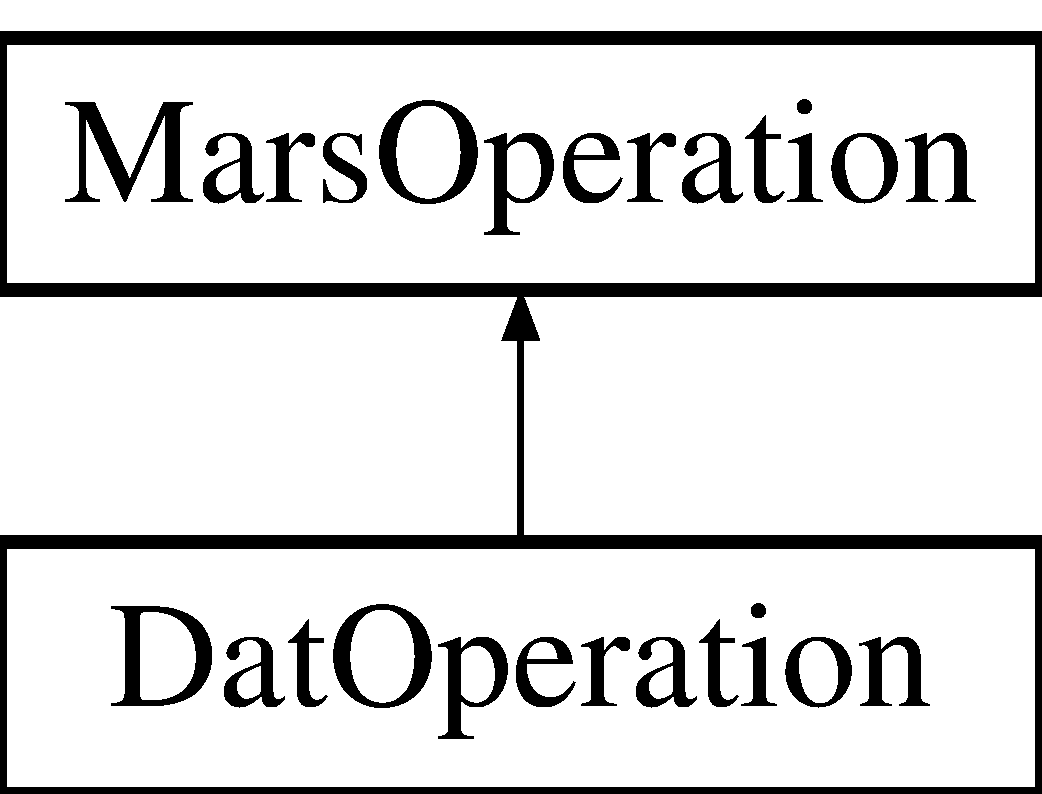
\includegraphics[height=2.000000cm]{classDatOperation}
\end{center}
\end{figure}
\subsection*{Public Member Functions}
\begin{DoxyCompactItemize}
\item 
\mbox{\Hypertarget{classDatOperation_a74db792f5ae0c4ea2686b984c671b677}\label{classDatOperation_a74db792f5ae0c4ea2686b984c671b677}} 
std\+::shared\+\_\+ptr$<$ \hyperlink{classProcessAction}{Process\+Action} $>$ {\bfseries run\+Operation} (\hyperlink{classOperationParamsInstructions}{Operation\+Params\+Instructions} $\ast$oper\+Params) override
\item 
\mbox{\Hypertarget{classDatOperation_a89124956b4683f8f9c5932de0ad239b1}\label{classDatOperation_a89124956b4683f8f9c5932de0ad239b1}} 
std\+::shared\+\_\+ptr$<$ \hyperlink{classProcessAction}{Process\+Action} $>$ {\bfseries run\+Operation} (\hyperlink{classOperationParamsMixed}{Operation\+Params\+Mixed} $\ast$oper\+Params) override
\end{DoxyCompactItemize}


\subsection{Detailed Description}
Class representing D\+AT operation 

The documentation for this class was generated from the following files\+:\begin{DoxyCompactItemize}
\item 
logic/mars/Dat\+Operation.\+h\item 
logic/mars/Dat\+Operation.\+cpp\end{DoxyCompactItemize}

\hypertarget{structCatch_1_1DecomposedExpression}{}\section{Catch\+:\+:Decomposed\+Expression Struct Reference}
\label{structCatch_1_1DecomposedExpression}\index{Catch\+::\+Decomposed\+Expression@{Catch\+::\+Decomposed\+Expression}}
Inheritance diagram for Catch\+:\+:Decomposed\+Expression\+:\begin{figure}[H]
\begin{center}
\leavevmode
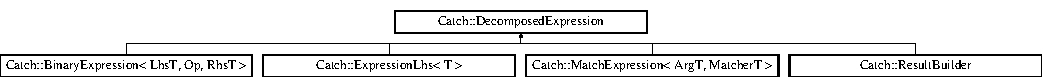
\includegraphics[height=1.029412cm]{structCatch_1_1DecomposedExpression}
\end{center}
\end{figure}
\subsection*{Public Member Functions}
\begin{DoxyCompactItemize}
\item 
\mbox{\Hypertarget{structCatch_1_1DecomposedExpression_a1c458ece47b71f093290dbdf9bb31fdb}\label{structCatch_1_1DecomposedExpression_a1c458ece47b71f093290dbdf9bb31fdb}} 
virtual bool {\bfseries is\+Binary\+Expression} () const
\item 
\mbox{\Hypertarget{structCatch_1_1DecomposedExpression_a9ce7f356dc96f11f80e40c82f5aa7e55}\label{structCatch_1_1DecomposedExpression_a9ce7f356dc96f11f80e40c82f5aa7e55}} 
virtual void {\bfseries reconstruct\+Expression} (std\+::string \&dest) const =0
\item 
\mbox{\Hypertarget{structCatch_1_1DecomposedExpression_aa2ce96ce31fef4afb21861bc0276edb9}\label{structCatch_1_1DecomposedExpression_aa2ce96ce31fef4afb21861bc0276edb9}} 
{\footnotesize template$<$typename T $>$ }\\S\+T\+A\+T\+I\+C\+\_\+\+A\+S\+S\+E\+R\+T\+\_\+\+Expression\+\_\+\+Too\+\_\+\+Complex\+\_\+\+Please\+\_\+\+Rewrite\+\_\+\+As\+\_\+\+Binary\+\_\+\+Comparison \& {\bfseries operator+} (T const \&)
\item 
\mbox{\Hypertarget{structCatch_1_1DecomposedExpression_aff39fb5d060abbd018c83b998d32c366}\label{structCatch_1_1DecomposedExpression_aff39fb5d060abbd018c83b998d32c366}} 
{\footnotesize template$<$typename T $>$ }\\S\+T\+A\+T\+I\+C\+\_\+\+A\+S\+S\+E\+R\+T\+\_\+\+Expression\+\_\+\+Too\+\_\+\+Complex\+\_\+\+Please\+\_\+\+Rewrite\+\_\+\+As\+\_\+\+Binary\+\_\+\+Comparison \& {\bfseries operator-\/} (T const \&)
\item 
\mbox{\Hypertarget{structCatch_1_1DecomposedExpression_afb5527e8e3cb8edca5113ec9801249d8}\label{structCatch_1_1DecomposedExpression_afb5527e8e3cb8edca5113ec9801249d8}} 
{\footnotesize template$<$typename T $>$ }\\S\+T\+A\+T\+I\+C\+\_\+\+A\+S\+S\+E\+R\+T\+\_\+\+Expression\+\_\+\+Too\+\_\+\+Complex\+\_\+\+Please\+\_\+\+Rewrite\+\_\+\+As\+\_\+\+Binary\+\_\+\+Comparison \& {\bfseries operator$\ast$} (T const \&)
\item 
\mbox{\Hypertarget{structCatch_1_1DecomposedExpression_a519d7e2363a92106e46371c9c04044a7}\label{structCatch_1_1DecomposedExpression_a519d7e2363a92106e46371c9c04044a7}} 
{\footnotesize template$<$typename T $>$ }\\S\+T\+A\+T\+I\+C\+\_\+\+A\+S\+S\+E\+R\+T\+\_\+\+Expression\+\_\+\+Too\+\_\+\+Complex\+\_\+\+Please\+\_\+\+Rewrite\+\_\+\+As\+\_\+\+Binary\+\_\+\+Comparison \& {\bfseries operator/} (T const \&)
\item 
\mbox{\Hypertarget{structCatch_1_1DecomposedExpression_a6584335aadaee847c9d06ca8f13a4477}\label{structCatch_1_1DecomposedExpression_a6584335aadaee847c9d06ca8f13a4477}} 
{\footnotesize template$<$typename T $>$ }\\S\+T\+A\+T\+I\+C\+\_\+\+A\+S\+S\+E\+R\+T\+\_\+\+Expression\+\_\+\+Too\+\_\+\+Complex\+\_\+\+Please\+\_\+\+Rewrite\+\_\+\+As\+\_\+\+Binary\+\_\+\+Comparison \& {\bfseries operator\%} (T const \&)
\item 
\mbox{\Hypertarget{structCatch_1_1DecomposedExpression_a14d913535796145b39101a16c0c490da}\label{structCatch_1_1DecomposedExpression_a14d913535796145b39101a16c0c490da}} 
{\footnotesize template$<$typename T $>$ }\\S\+T\+A\+T\+I\+C\+\_\+\+A\+S\+S\+E\+R\+T\+\_\+\+Expression\+\_\+\+Too\+\_\+\+Complex\+\_\+\+Please\+\_\+\+Rewrite\+\_\+\+As\+\_\+\+Binary\+\_\+\+Comparison \& {\bfseries operator\&\&} (T const \&)
\item 
\mbox{\Hypertarget{structCatch_1_1DecomposedExpression_ab4800d277290088fea9c594cfdd4f1c7}\label{structCatch_1_1DecomposedExpression_ab4800d277290088fea9c594cfdd4f1c7}} 
{\footnotesize template$<$typename T $>$ }\\S\+T\+A\+T\+I\+C\+\_\+\+A\+S\+S\+E\+R\+T\+\_\+\+Expression\+\_\+\+Too\+\_\+\+Complex\+\_\+\+Please\+\_\+\+Rewrite\+\_\+\+As\+\_\+\+Binary\+\_\+\+Comparison \& {\bfseries operator$\vert$$\vert$} (T const \&)
\end{DoxyCompactItemize}


The documentation for this struct was generated from the following file\+:\begin{DoxyCompactItemize}
\item 
test\+\_\+cases/catch.\+hpp\end{DoxyCompactItemize}

\hypertarget{classDirectInstructionModifier}{}\section{Direct\+Instruction\+Modifier Class Reference}
\label{classDirectInstructionModifier}\index{Direct\+Instruction\+Modifier@{Direct\+Instruction\+Modifier}}
Inheritance diagram for Direct\+Instruction\+Modifier\+:\begin{figure}[H]
\begin{center}
\leavevmode
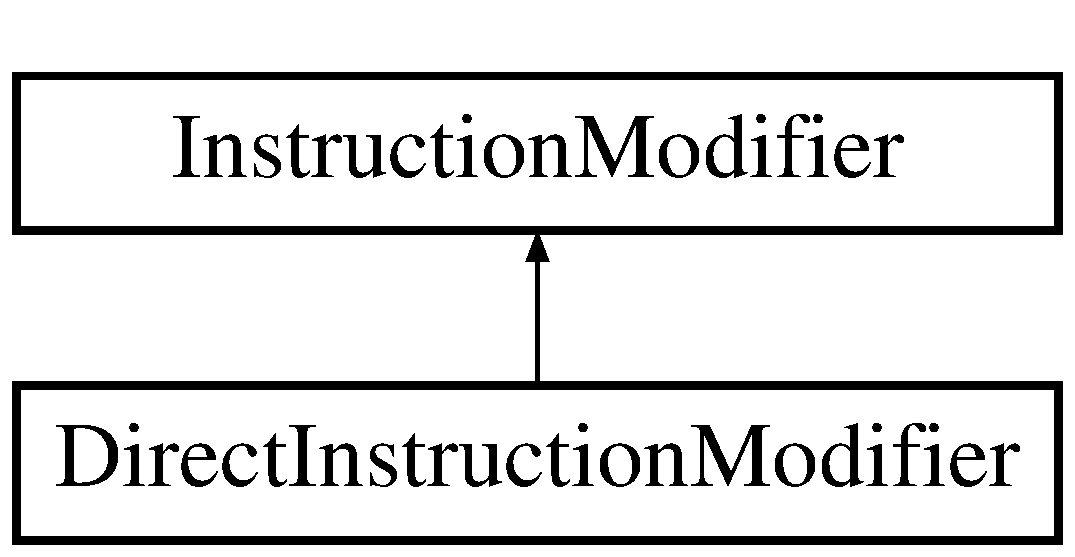
\includegraphics[height=2.000000cm]{classDirectInstructionModifier}
\end{center}
\end{figure}
\subsection*{Public Member Functions}
\begin{DoxyCompactItemize}
\item 
\mbox{\Hypertarget{classDirectInstructionModifier_a1b6c16747753e64bfaa0e1da3a4e96ad}\label{classDirectInstructionModifier_a1b6c16747753e64bfaa0e1da3a4e96ad}} 
boost\+::optional$<$ \hyperlink{classInstruction}{Instruction} $>$ {\bfseries find\+Target\+Instruction} (\hyperlink{classMemoryIndex}{Memory\+Index} \&m\+Index, const std\+::vector$<$ \hyperlink{classInstruction}{Instruction} $>$ memory\+Array) override
\item 
\mbox{\Hypertarget{classDirectInstructionModifier_a13e4d21fcbb0e17f440dd14047599ebb}\label{classDirectInstructionModifier_a13e4d21fcbb0e17f440dd14047599ebb}} 
std\+::shared\+\_\+ptr$<$ \hyperlink{classInstructionModifier}{Instruction\+Modifier} $>$ {\bfseries clone} () const override
\end{DoxyCompactItemize}


The documentation for this class was generated from the following files\+:\begin{DoxyCompactItemize}
\item 
logic/parser/Direct\+Instruction\+Modifier.\+h\item 
logic/parser/Direct\+Instruction\+Modifier.\+cpp\end{DoxyCompactItemize}

\hypertarget{structCatch_1_1Matchers_1_1StdString_1_1EndsWithMatcher}{}\section{Catch\+:\+:Matchers\+:\+:Std\+String\+:\+:Ends\+With\+Matcher Struct Reference}
\label{structCatch_1_1Matchers_1_1StdString_1_1EndsWithMatcher}\index{Catch\+::\+Matchers\+::\+Std\+String\+::\+Ends\+With\+Matcher@{Catch\+::\+Matchers\+::\+Std\+String\+::\+Ends\+With\+Matcher}}
Inheritance diagram for Catch\+:\+:Matchers\+:\+:Std\+String\+:\+:Ends\+With\+Matcher\+:\begin{figure}[H]
\begin{center}
\leavevmode
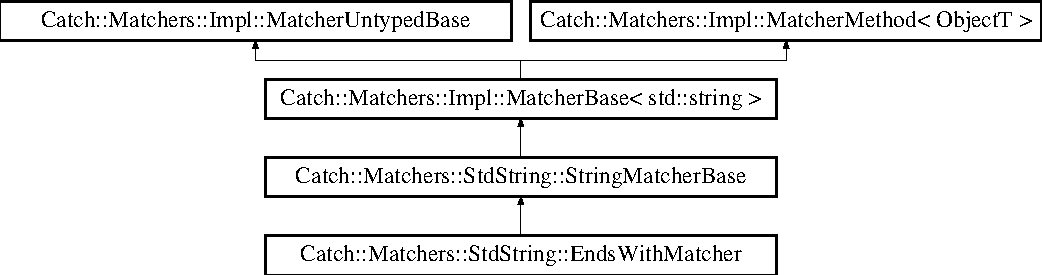
\includegraphics[height=3.696370cm]{structCatch_1_1Matchers_1_1StdString_1_1EndsWithMatcher}
\end{center}
\end{figure}
\subsection*{Public Member Functions}
\begin{DoxyCompactItemize}
\item 
\mbox{\Hypertarget{structCatch_1_1Matchers_1_1StdString_1_1EndsWithMatcher_aa5ec700b4629562f74f362080accfd7b}\label{structCatch_1_1Matchers_1_1StdString_1_1EndsWithMatcher_aa5ec700b4629562f74f362080accfd7b}} 
{\bfseries Ends\+With\+Matcher} (\hyperlink{structCatch_1_1Matchers_1_1StdString_1_1CasedString}{Cased\+String} const \&comparator)
\item 
\mbox{\Hypertarget{structCatch_1_1Matchers_1_1StdString_1_1EndsWithMatcher_a21c6dc68e30716d5c718f4f8c3186af1}\label{structCatch_1_1Matchers_1_1StdString_1_1EndsWithMatcher_a21c6dc68e30716d5c718f4f8c3186af1}} 
virtual bool {\bfseries match} (std\+::string const \&source) const C\+A\+T\+C\+H\+\_\+\+O\+V\+E\+R\+R\+I\+DE
\end{DoxyCompactItemize}
\subsection*{Additional Inherited Members}


The documentation for this struct was generated from the following file\+:\begin{DoxyCompactItemize}
\item 
test\+\_\+cases/catch.\+hpp\end{DoxyCompactItemize}

\hypertarget{structCatch_1_1Matchers_1_1StdString_1_1EqualsMatcher}{}\section{Catch\+:\+:Matchers\+:\+:Std\+String\+:\+:Equals\+Matcher Struct Reference}
\label{structCatch_1_1Matchers_1_1StdString_1_1EqualsMatcher}\index{Catch\+::\+Matchers\+::\+Std\+String\+::\+Equals\+Matcher@{Catch\+::\+Matchers\+::\+Std\+String\+::\+Equals\+Matcher}}
Inheritance diagram for Catch\+:\+:Matchers\+:\+:Std\+String\+:\+:Equals\+Matcher\+:\begin{figure}[H]
\begin{center}
\leavevmode
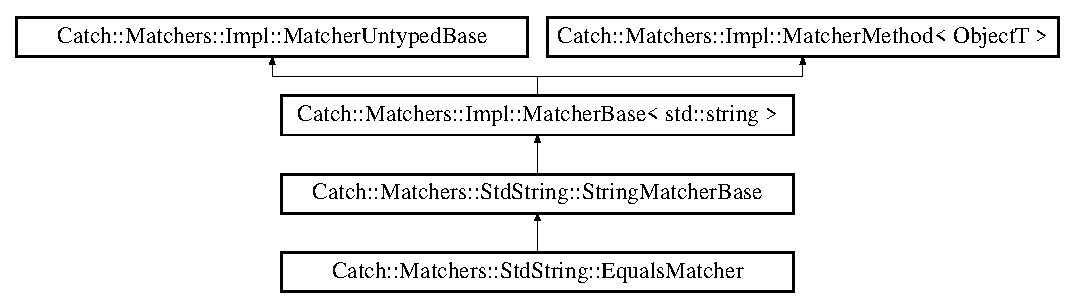
\includegraphics[height=3.696370cm]{structCatch_1_1Matchers_1_1StdString_1_1EqualsMatcher}
\end{center}
\end{figure}
\subsection*{Public Member Functions}
\begin{DoxyCompactItemize}
\item 
\mbox{\Hypertarget{structCatch_1_1Matchers_1_1StdString_1_1EqualsMatcher_ab740f1fb2310e9fe3fed5134d4c7e4c8}\label{structCatch_1_1Matchers_1_1StdString_1_1EqualsMatcher_ab740f1fb2310e9fe3fed5134d4c7e4c8}} 
{\bfseries Equals\+Matcher} (\hyperlink{structCatch_1_1Matchers_1_1StdString_1_1CasedString}{Cased\+String} const \&comparator)
\item 
\mbox{\Hypertarget{structCatch_1_1Matchers_1_1StdString_1_1EqualsMatcher_a2aeaac3c0efb8422643cd1b155256213}\label{structCatch_1_1Matchers_1_1StdString_1_1EqualsMatcher_a2aeaac3c0efb8422643cd1b155256213}} 
virtual bool {\bfseries match} (std\+::string const \&source) const C\+A\+T\+C\+H\+\_\+\+O\+V\+E\+R\+R\+I\+DE
\end{DoxyCompactItemize}
\subsection*{Additional Inherited Members}


The documentation for this struct was generated from the following file\+:\begin{DoxyCompactItemize}
\item 
test\+\_\+cases/catch.\+hpp\end{DoxyCompactItemize}

\hypertarget{structCatch_1_1Matchers_1_1Vector_1_1EqualsMatcher}{}\section{Catch\+:\+:Matchers\+:\+:Vector\+:\+:Equals\+Matcher$<$ T $>$ Struct Template Reference}
\label{structCatch_1_1Matchers_1_1Vector_1_1EqualsMatcher}\index{Catch\+::\+Matchers\+::\+Vector\+::\+Equals\+Matcher$<$ T $>$@{Catch\+::\+Matchers\+::\+Vector\+::\+Equals\+Matcher$<$ T $>$}}
Inheritance diagram for Catch\+:\+:Matchers\+:\+:Vector\+:\+:Equals\+Matcher$<$ T $>$\+:\begin{figure}[H]
\begin{center}
\leavevmode
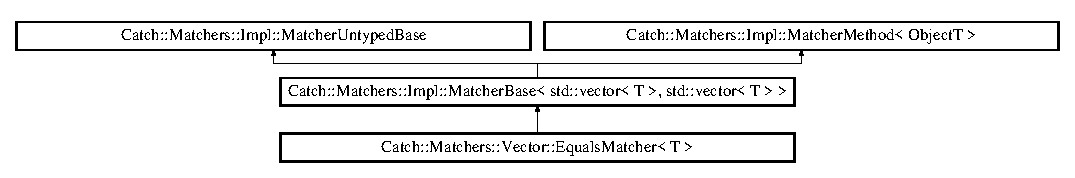
\includegraphics[height=1.944444cm]{structCatch_1_1Matchers_1_1Vector_1_1EqualsMatcher}
\end{center}
\end{figure}
\subsection*{Public Member Functions}
\begin{DoxyCompactItemize}
\item 
\mbox{\Hypertarget{structCatch_1_1Matchers_1_1Vector_1_1EqualsMatcher_a3846c47780d1991dcfe87aefded98008}\label{structCatch_1_1Matchers_1_1Vector_1_1EqualsMatcher_a3846c47780d1991dcfe87aefded98008}} 
{\bfseries Equals\+Matcher} (std\+::vector$<$ T $>$ const \&comparator)
\item 
\mbox{\Hypertarget{structCatch_1_1Matchers_1_1Vector_1_1EqualsMatcher_aca444c319d1b4c6f538faf9c4735da04}\label{structCatch_1_1Matchers_1_1Vector_1_1EqualsMatcher_aca444c319d1b4c6f538faf9c4735da04}} 
bool {\bfseries match} (std\+::vector$<$ T $>$ const \&v) const C\+A\+T\+C\+H\+\_\+\+O\+V\+E\+R\+R\+I\+DE
\item 
\mbox{\Hypertarget{structCatch_1_1Matchers_1_1Vector_1_1EqualsMatcher_aca79ade26f4a75b2a57005067e086e35}\label{structCatch_1_1Matchers_1_1Vector_1_1EqualsMatcher_aca79ade26f4a75b2a57005067e086e35}} 
virtual std\+::string {\bfseries describe} () const C\+A\+T\+C\+H\+\_\+\+O\+V\+E\+R\+R\+I\+DE
\end{DoxyCompactItemize}
\subsection*{Public Attributes}
\begin{DoxyCompactItemize}
\item 
\mbox{\Hypertarget{structCatch_1_1Matchers_1_1Vector_1_1EqualsMatcher_a56f7aa6f110a12b1b9aeb0cabbc9d755}\label{structCatch_1_1Matchers_1_1Vector_1_1EqualsMatcher_a56f7aa6f110a12b1b9aeb0cabbc9d755}} 
std\+::vector$<$ T $>$ const  \& {\bfseries m\+\_\+comparator}
\end{DoxyCompactItemize}
\subsection*{Additional Inherited Members}


The documentation for this struct was generated from the following file\+:\begin{DoxyCompactItemize}
\item 
test\+\_\+cases/catch.\+hpp\end{DoxyCompactItemize}

\hypertarget{classCatch_1_1Internal_1_1Evaluator}{}\section{Catch\+:\+:Internal\+:\+:Evaluator$<$ T1, T2, Op $>$ Class Template Reference}
\label{classCatch_1_1Internal_1_1Evaluator}\index{Catch\+::\+Internal\+::\+Evaluator$<$ T1, T2, Op $>$@{Catch\+::\+Internal\+::\+Evaluator$<$ T1, T2, Op $>$}}


The documentation for this class was generated from the following file\+:\begin{DoxyCompactItemize}
\item 
test\+\_\+cases/catch.\+hpp\end{DoxyCompactItemize}

\hypertarget{structCatch_1_1Internal_1_1Evaluator_3_01T1_00_01T2_00_01IsEqualTo_01_4}{}\section{Catch\+:\+:Internal\+:\+:Evaluator$<$ T1, T2, Is\+Equal\+To $>$ Struct Template Reference}
\label{structCatch_1_1Internal_1_1Evaluator_3_01T1_00_01T2_00_01IsEqualTo_01_4}\index{Catch\+::\+Internal\+::\+Evaluator$<$ T1, T2, Is\+Equal\+To $>$@{Catch\+::\+Internal\+::\+Evaluator$<$ T1, T2, Is\+Equal\+To $>$}}
\subsection*{Static Public Member Functions}
\begin{DoxyCompactItemize}
\item 
\mbox{\Hypertarget{structCatch_1_1Internal_1_1Evaluator_3_01T1_00_01T2_00_01IsEqualTo_01_4_a166b2b7849247397e63fb2940481b217}\label{structCatch_1_1Internal_1_1Evaluator_3_01T1_00_01T2_00_01IsEqualTo_01_4_a166b2b7849247397e63fb2940481b217}} 
static bool {\bfseries evaluate} (T1 const \&lhs, T2 const \&rhs)
\end{DoxyCompactItemize}


The documentation for this struct was generated from the following file\+:\begin{DoxyCompactItemize}
\item 
test\+\_\+cases/catch.\+hpp\end{DoxyCompactItemize}

\hypertarget{structCatch_1_1Internal_1_1Evaluator_3_01T1_00_01T2_00_01IsGreaterThan_01_4}{}\section{Catch\+:\+:Internal\+:\+:Evaluator$<$ T1, T2, Is\+Greater\+Than $>$ Struct Template Reference}
\label{structCatch_1_1Internal_1_1Evaluator_3_01T1_00_01T2_00_01IsGreaterThan_01_4}\index{Catch\+::\+Internal\+::\+Evaluator$<$ T1, T2, Is\+Greater\+Than $>$@{Catch\+::\+Internal\+::\+Evaluator$<$ T1, T2, Is\+Greater\+Than $>$}}
\subsection*{Static Public Member Functions}
\begin{DoxyCompactItemize}
\item 
\mbox{\Hypertarget{structCatch_1_1Internal_1_1Evaluator_3_01T1_00_01T2_00_01IsGreaterThan_01_4_a55745f74f09ac5c61bd3d592ca5560af}\label{structCatch_1_1Internal_1_1Evaluator_3_01T1_00_01T2_00_01IsGreaterThan_01_4_a55745f74f09ac5c61bd3d592ca5560af}} 
static bool {\bfseries evaluate} (T1 const \&lhs, T2 const \&rhs)
\end{DoxyCompactItemize}


The documentation for this struct was generated from the following file\+:\begin{DoxyCompactItemize}
\item 
test\+\_\+cases/catch.\+hpp\end{DoxyCompactItemize}

\hypertarget{structCatch_1_1Internal_1_1Evaluator_3_01T1_00_01T2_00_01IsGreaterThanOrEqualTo_01_4}{}\section{Catch\+:\+:Internal\+:\+:Evaluator$<$ T1, T2, Is\+Greater\+Than\+Or\+Equal\+To $>$ Struct Template Reference}
\label{structCatch_1_1Internal_1_1Evaluator_3_01T1_00_01T2_00_01IsGreaterThanOrEqualTo_01_4}\index{Catch\+::\+Internal\+::\+Evaluator$<$ T1, T2, Is\+Greater\+Than\+Or\+Equal\+To $>$@{Catch\+::\+Internal\+::\+Evaluator$<$ T1, T2, Is\+Greater\+Than\+Or\+Equal\+To $>$}}
\subsection*{Static Public Member Functions}
\begin{DoxyCompactItemize}
\item 
\mbox{\Hypertarget{structCatch_1_1Internal_1_1Evaluator_3_01T1_00_01T2_00_01IsGreaterThanOrEqualTo_01_4_a5ba107c6da4292b6492a0e5e906f9484}\label{structCatch_1_1Internal_1_1Evaluator_3_01T1_00_01T2_00_01IsGreaterThanOrEqualTo_01_4_a5ba107c6da4292b6492a0e5e906f9484}} 
static bool {\bfseries evaluate} (T1 const \&lhs, T2 const \&rhs)
\end{DoxyCompactItemize}


The documentation for this struct was generated from the following file\+:\begin{DoxyCompactItemize}
\item 
test\+\_\+cases/catch.\+hpp\end{DoxyCompactItemize}

\hypertarget{structCatch_1_1Internal_1_1Evaluator_3_01T1_00_01T2_00_01IsLessThan_01_4}{}\section{Catch\+:\+:Internal\+:\+:Evaluator$<$ T1, T2, Is\+Less\+Than $>$ Struct Template Reference}
\label{structCatch_1_1Internal_1_1Evaluator_3_01T1_00_01T2_00_01IsLessThan_01_4}\index{Catch\+::\+Internal\+::\+Evaluator$<$ T1, T2, Is\+Less\+Than $>$@{Catch\+::\+Internal\+::\+Evaluator$<$ T1, T2, Is\+Less\+Than $>$}}
\subsection*{Static Public Member Functions}
\begin{DoxyCompactItemize}
\item 
\mbox{\Hypertarget{structCatch_1_1Internal_1_1Evaluator_3_01T1_00_01T2_00_01IsLessThan_01_4_a75b2bcf80ce6f90218c145e2c3293d75}\label{structCatch_1_1Internal_1_1Evaluator_3_01T1_00_01T2_00_01IsLessThan_01_4_a75b2bcf80ce6f90218c145e2c3293d75}} 
static bool {\bfseries evaluate} (T1 const \&lhs, T2 const \&rhs)
\end{DoxyCompactItemize}


The documentation for this struct was generated from the following file\+:\begin{DoxyCompactItemize}
\item 
test\+\_\+cases/catch.\+hpp\end{DoxyCompactItemize}

\hypertarget{structCatch_1_1Internal_1_1Evaluator_3_01T1_00_01T2_00_01IsLessThanOrEqualTo_01_4}{}\section{Catch\+:\+:Internal\+:\+:Evaluator$<$ T1, T2, Is\+Less\+Than\+Or\+Equal\+To $>$ Struct Template Reference}
\label{structCatch_1_1Internal_1_1Evaluator_3_01T1_00_01T2_00_01IsLessThanOrEqualTo_01_4}\index{Catch\+::\+Internal\+::\+Evaluator$<$ T1, T2, Is\+Less\+Than\+Or\+Equal\+To $>$@{Catch\+::\+Internal\+::\+Evaluator$<$ T1, T2, Is\+Less\+Than\+Or\+Equal\+To $>$}}
\subsection*{Static Public Member Functions}
\begin{DoxyCompactItemize}
\item 
\mbox{\Hypertarget{structCatch_1_1Internal_1_1Evaluator_3_01T1_00_01T2_00_01IsLessThanOrEqualTo_01_4_adf269a597e4d82d69f29bcb516297b9b}\label{structCatch_1_1Internal_1_1Evaluator_3_01T1_00_01T2_00_01IsLessThanOrEqualTo_01_4_adf269a597e4d82d69f29bcb516297b9b}} 
static bool {\bfseries evaluate} (T1 const \&lhs, T2 const \&rhs)
\end{DoxyCompactItemize}


The documentation for this struct was generated from the following file\+:\begin{DoxyCompactItemize}
\item 
test\+\_\+cases/catch.\+hpp\end{DoxyCompactItemize}

\hypertarget{structCatch_1_1Internal_1_1Evaluator_3_01T1_00_01T2_00_01IsNotEqualTo_01_4}{}\section{Catch\+:\+:Internal\+:\+:Evaluator$<$ T1, T2, Is\+Not\+Equal\+To $>$ Struct Template Reference}
\label{structCatch_1_1Internal_1_1Evaluator_3_01T1_00_01T2_00_01IsNotEqualTo_01_4}\index{Catch\+::\+Internal\+::\+Evaluator$<$ T1, T2, Is\+Not\+Equal\+To $>$@{Catch\+::\+Internal\+::\+Evaluator$<$ T1, T2, Is\+Not\+Equal\+To $>$}}
\subsection*{Static Public Member Functions}
\begin{DoxyCompactItemize}
\item 
\mbox{\Hypertarget{structCatch_1_1Internal_1_1Evaluator_3_01T1_00_01T2_00_01IsNotEqualTo_01_4_a956a12d0f4a7dceb5a1ce914421ff945}\label{structCatch_1_1Internal_1_1Evaluator_3_01T1_00_01T2_00_01IsNotEqualTo_01_4_a956a12d0f4a7dceb5a1ce914421ff945}} 
static bool {\bfseries evaluate} (T1 const \&lhs, T2 const \&rhs)
\end{DoxyCompactItemize}


The documentation for this struct was generated from the following file\+:\begin{DoxyCompactItemize}
\item 
test\+\_\+cases/catch.\+hpp\end{DoxyCompactItemize}

\hypertarget{classCatch_1_1ExceptionTranslatorRegistrar}{}\section{Catch\+:\+:Exception\+Translator\+Registrar Class Reference}
\label{classCatch_1_1ExceptionTranslatorRegistrar}\index{Catch\+::\+Exception\+Translator\+Registrar@{Catch\+::\+Exception\+Translator\+Registrar}}
\subsection*{Public Member Functions}
\begin{DoxyCompactItemize}
\item 
\mbox{\Hypertarget{classCatch_1_1ExceptionTranslatorRegistrar_aa73229de911f26b1df6c6c87c4d9e04e}\label{classCatch_1_1ExceptionTranslatorRegistrar_aa73229de911f26b1df6c6c87c4d9e04e}} 
{\footnotesize template$<$typename T $>$ }\\{\bfseries Exception\+Translator\+Registrar} (std\+::string($\ast$translate\+Function)(T \&))
\end{DoxyCompactItemize}


The documentation for this class was generated from the following file\+:\begin{DoxyCompactItemize}
\item 
test\+\_\+cases/catch.\+hpp\end{DoxyCompactItemize}

\hypertarget{classCatch_1_1ExpressionLhs}{}\section{Catch\+:\+:Expression\+Lhs$<$ T $>$ Class Template Reference}
\label{classCatch_1_1ExpressionLhs}\index{Catch\+::\+Expression\+Lhs$<$ T $>$@{Catch\+::\+Expression\+Lhs$<$ T $>$}}
Inheritance diagram for Catch\+:\+:Expression\+Lhs$<$ T $>$\+:\begin{figure}[H]
\begin{center}
\leavevmode
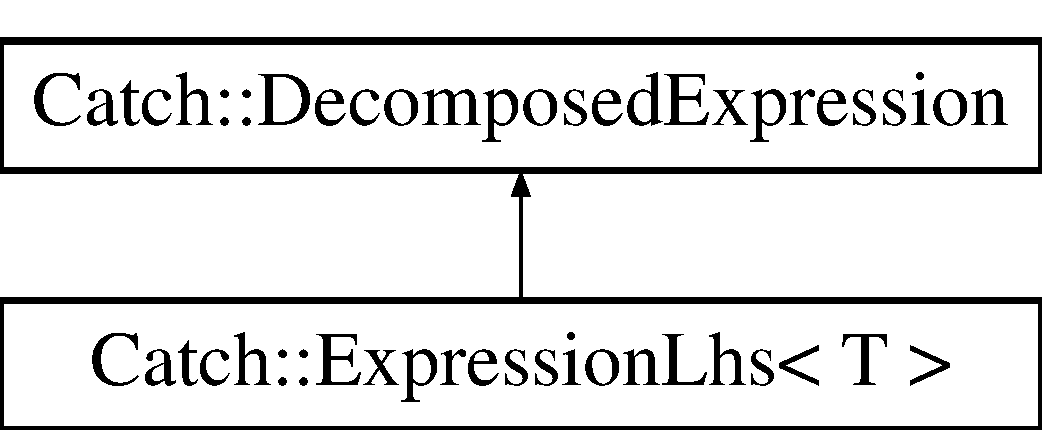
\includegraphics[height=2.000000cm]{classCatch_1_1ExpressionLhs}
\end{center}
\end{figure}
\subsection*{Public Member Functions}
\begin{DoxyCompactItemize}
\item 
\mbox{\Hypertarget{classCatch_1_1ExpressionLhs_aa829588def6146a94fb75de9c4cc482a}\label{classCatch_1_1ExpressionLhs_aa829588def6146a94fb75de9c4cc482a}} 
{\bfseries Expression\+Lhs} (\hyperlink{classCatch_1_1ResultBuilder}{Result\+Builder} \&rb, T lhs)
\item 
\mbox{\Hypertarget{classCatch_1_1ExpressionLhs_a60d50fe8adcaabcb7c93747ddbae5993}\label{classCatch_1_1ExpressionLhs_a60d50fe8adcaabcb7c93747ddbae5993}} 
\hyperlink{classCatch_1_1ExpressionLhs}{Expression\+Lhs} \& {\bfseries operator=} (const \hyperlink{classCatch_1_1ExpressionLhs}{Expression\+Lhs} \&)
\item 
\mbox{\Hypertarget{classCatch_1_1ExpressionLhs_abebe4afc079c91ae548ab8fdba6c77f2}\label{classCatch_1_1ExpressionLhs_abebe4afc079c91ae548ab8fdba6c77f2}} 
{\footnotesize template$<$typename RhsT $>$ }\\\hyperlink{classCatch_1_1BinaryExpression}{Binary\+Expression}$<$ T, Internal\+::\+Is\+Equal\+To, RhsT const  \& $>$ {\bfseries operator==} (RhsT const \&rhs)
\item 
\mbox{\Hypertarget{classCatch_1_1ExpressionLhs_a3bc08bb2b9c27678e2628faa73645144}\label{classCatch_1_1ExpressionLhs_a3bc08bb2b9c27678e2628faa73645144}} 
{\footnotesize template$<$typename RhsT $>$ }\\\hyperlink{classCatch_1_1BinaryExpression}{Binary\+Expression}$<$ T, Internal\+::\+Is\+Not\+Equal\+To, RhsT const  \& $>$ {\bfseries operator!=} (RhsT const \&rhs)
\item 
\mbox{\Hypertarget{classCatch_1_1ExpressionLhs_a919c48e52ff1be5f7329920d4da8e92f}\label{classCatch_1_1ExpressionLhs_a919c48e52ff1be5f7329920d4da8e92f}} 
{\footnotesize template$<$typename RhsT $>$ }\\\hyperlink{classCatch_1_1BinaryExpression}{Binary\+Expression}$<$ T, Internal\+::\+Is\+Less\+Than, RhsT const  \& $>$ {\bfseries operator$<$} (RhsT const \&rhs)
\item 
\mbox{\Hypertarget{classCatch_1_1ExpressionLhs_a52981d92ec6aad872660ae7df1abb33a}\label{classCatch_1_1ExpressionLhs_a52981d92ec6aad872660ae7df1abb33a}} 
{\footnotesize template$<$typename RhsT $>$ }\\\hyperlink{classCatch_1_1BinaryExpression}{Binary\+Expression}$<$ T, Internal\+::\+Is\+Greater\+Than, RhsT const  \& $>$ {\bfseries operator$>$} (RhsT const \&rhs)
\item 
\mbox{\Hypertarget{classCatch_1_1ExpressionLhs_a1d10974a581c67cc400cd6cdd36b0000}\label{classCatch_1_1ExpressionLhs_a1d10974a581c67cc400cd6cdd36b0000}} 
{\footnotesize template$<$typename RhsT $>$ }\\\hyperlink{classCatch_1_1BinaryExpression}{Binary\+Expression}$<$ T, Internal\+::\+Is\+Less\+Than\+Or\+Equal\+To, RhsT const  \& $>$ {\bfseries operator$<$=} (RhsT const \&rhs)
\item 
\mbox{\Hypertarget{classCatch_1_1ExpressionLhs_a3387a494cb6b699a6c0162c79f7f533c}\label{classCatch_1_1ExpressionLhs_a3387a494cb6b699a6c0162c79f7f533c}} 
{\footnotesize template$<$typename RhsT $>$ }\\\hyperlink{classCatch_1_1BinaryExpression}{Binary\+Expression}$<$ T, Internal\+::\+Is\+Greater\+Than\+Or\+Equal\+To, RhsT const  \& $>$ {\bfseries operator$>$=} (RhsT const \&rhs)
\item 
\mbox{\Hypertarget{classCatch_1_1ExpressionLhs_ab803185079504a65b0af95f7c9669351}\label{classCatch_1_1ExpressionLhs_ab803185079504a65b0af95f7c9669351}} 
\hyperlink{classCatch_1_1BinaryExpression}{Binary\+Expression}$<$ T, Internal\+::\+Is\+Equal\+To, bool $>$ {\bfseries operator==} (bool rhs)
\item 
\mbox{\Hypertarget{classCatch_1_1ExpressionLhs_a1f3ff934880623f12a4cbd9725397ccf}\label{classCatch_1_1ExpressionLhs_a1f3ff934880623f12a4cbd9725397ccf}} 
\hyperlink{classCatch_1_1BinaryExpression}{Binary\+Expression}$<$ T, Internal\+::\+Is\+Not\+Equal\+To, bool $>$ {\bfseries operator!=} (bool rhs)
\item 
\mbox{\Hypertarget{classCatch_1_1ExpressionLhs_a13d2551a927790284fb5ddf1ee2c9079}\label{classCatch_1_1ExpressionLhs_a13d2551a927790284fb5ddf1ee2c9079}} 
void {\bfseries end\+Expression} ()
\item 
\mbox{\Hypertarget{classCatch_1_1ExpressionLhs_a7684a053e8e88a4be475a536252630da}\label{classCatch_1_1ExpressionLhs_a7684a053e8e88a4be475a536252630da}} 
virtual void {\bfseries reconstruct\+Expression} (std\+::string \&dest) const C\+A\+T\+C\+H\+\_\+\+O\+V\+E\+R\+R\+I\+DE
\end{DoxyCompactItemize}


The documentation for this class was generated from the following file\+:\begin{DoxyCompactItemize}
\item 
test\+\_\+cases/catch.\+hpp\end{DoxyCompactItemize}

\hypertarget{structCatch_1_1Detail_1_1FalseType}{}\section{Catch\+:\+:Detail\+:\+:False\+Type Struct Reference}
\label{structCatch_1_1Detail_1_1FalseType}\index{Catch\+::\+Detail\+::\+False\+Type@{Catch\+::\+Detail\+::\+False\+Type}}
\subsection*{Public Attributes}
\begin{DoxyCompactItemize}
\item 
\mbox{\Hypertarget{structCatch_1_1Detail_1_1FalseType_abc1a730e197d6f7750ae8aaf47b63477}\label{structCatch_1_1Detail_1_1FalseType_abc1a730e197d6f7750ae8aaf47b63477}} 
char {\bfseries sizer} \mbox{[}2\mbox{]}
\end{DoxyCompactItemize}


The documentation for this struct was generated from the following file\+:\begin{DoxyCompactItemize}
\item 
test\+\_\+cases/catch.\+hpp\end{DoxyCompactItemize}

\hypertarget{structCatch_1_1IContext}{}\section{Catch\+:\+:I\+Context Struct Reference}
\label{structCatch_1_1IContext}\index{Catch\+::\+I\+Context@{Catch\+::\+I\+Context}}
Inheritance diagram for Catch\+:\+:I\+Context\+:\begin{figure}[H]
\begin{center}
\leavevmode
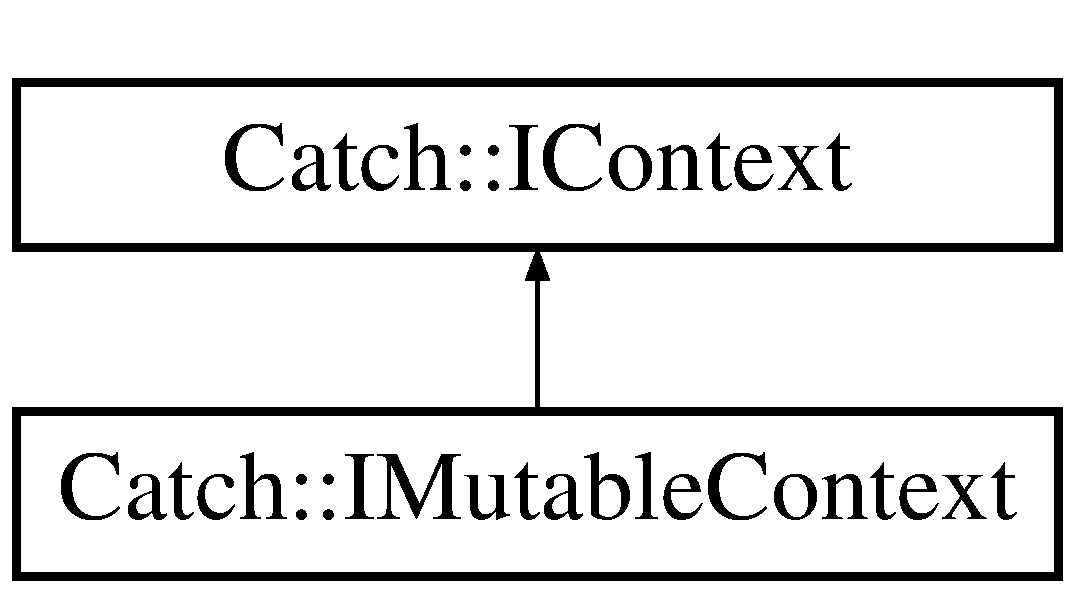
\includegraphics[height=2.000000cm]{structCatch_1_1IContext}
\end{center}
\end{figure}
\subsection*{Public Member Functions}
\begin{DoxyCompactItemize}
\item 
\mbox{\Hypertarget{structCatch_1_1IContext_a684e4ae71d1fdf3060c352ecde1d122f}\label{structCatch_1_1IContext_a684e4ae71d1fdf3060c352ecde1d122f}} 
virtual \hyperlink{structCatch_1_1IResultCapture}{I\+Result\+Capture} $\ast$ {\bfseries get\+Result\+Capture} ()=0
\item 
\mbox{\Hypertarget{structCatch_1_1IContext_af088415dde18d039ed5a2f95b02767c6}\label{structCatch_1_1IContext_af088415dde18d039ed5a2f95b02767c6}} 
virtual \hyperlink{structCatch_1_1IRunner}{I\+Runner} $\ast$ {\bfseries get\+Runner} ()=0
\item 
\mbox{\Hypertarget{structCatch_1_1IContext_a43e07088db43299ba129fbe6d3106e95}\label{structCatch_1_1IContext_a43e07088db43299ba129fbe6d3106e95}} 
virtual size\+\_\+t {\bfseries get\+Generator\+Index} (std\+::string const \&file\+Info, size\+\_\+t total\+Size)=0
\item 
\mbox{\Hypertarget{structCatch_1_1IContext_a806f7c4ed24d51adae90418e661b24b7}\label{structCatch_1_1IContext_a806f7c4ed24d51adae90418e661b24b7}} 
virtual bool {\bfseries advance\+Generators\+For\+Current\+Test} ()=0
\item 
\mbox{\Hypertarget{structCatch_1_1IContext_aee81c415899262e096ad8d6f686fa365}\label{structCatch_1_1IContext_aee81c415899262e096ad8d6f686fa365}} 
virtual \hyperlink{classCatch_1_1Ptr}{Ptr}$<$ I\+Config const  $>$ {\bfseries get\+Config} () const =0
\end{DoxyCompactItemize}


The documentation for this struct was generated from the following file\+:\begin{DoxyCompactItemize}
\item 
test\+\_\+cases/catch.\+hpp\end{DoxyCompactItemize}

\hypertarget{structCatch_1_1IExceptionTranslator}{}\section{Catch\+:\+:I\+Exception\+Translator Struct Reference}
\label{structCatch_1_1IExceptionTranslator}\index{Catch\+::\+I\+Exception\+Translator@{Catch\+::\+I\+Exception\+Translator}}
\subsection*{Public Member Functions}
\begin{DoxyCompactItemize}
\item 
\mbox{\Hypertarget{structCatch_1_1IExceptionTranslator_a2a554b96ed5ed411e7c796b6b42837a5}\label{structCatch_1_1IExceptionTranslator_a2a554b96ed5ed411e7c796b6b42837a5}} 
virtual std\+::string {\bfseries translate} (Exception\+Translators\+::const\+\_\+iterator it, Exception\+Translators\+::const\+\_\+iterator it\+End) const =0
\end{DoxyCompactItemize}


The documentation for this struct was generated from the following file\+:\begin{DoxyCompactItemize}
\item 
test\+\_\+cases/catch.\+hpp\end{DoxyCompactItemize}

\hypertarget{structCatch_1_1IExceptionTranslatorRegistry}{}\section{Catch\+:\+:I\+Exception\+Translator\+Registry Struct Reference}
\label{structCatch_1_1IExceptionTranslatorRegistry}\index{Catch\+::\+I\+Exception\+Translator\+Registry@{Catch\+::\+I\+Exception\+Translator\+Registry}}
\subsection*{Public Member Functions}
\begin{DoxyCompactItemize}
\item 
\mbox{\Hypertarget{structCatch_1_1IExceptionTranslatorRegistry_af76ae8c331a17f2a94c9720bc0d686bb}\label{structCatch_1_1IExceptionTranslatorRegistry_af76ae8c331a17f2a94c9720bc0d686bb}} 
virtual std\+::string {\bfseries translate\+Active\+Exception} () const =0
\end{DoxyCompactItemize}


The documentation for this struct was generated from the following file\+:\begin{DoxyCompactItemize}
\item 
test\+\_\+cases/catch.\+hpp\end{DoxyCompactItemize}

\hypertarget{structCatch_1_1IGenerator}{}\section{Catch\+:\+:I\+Generator$<$ T $>$ Struct Template Reference}
\label{structCatch_1_1IGenerator}\index{Catch\+::\+I\+Generator$<$ T $>$@{Catch\+::\+I\+Generator$<$ T $>$}}
Inheritance diagram for Catch\+:\+:I\+Generator$<$ T $>$\+:\begin{figure}[H]
\begin{center}
\leavevmode
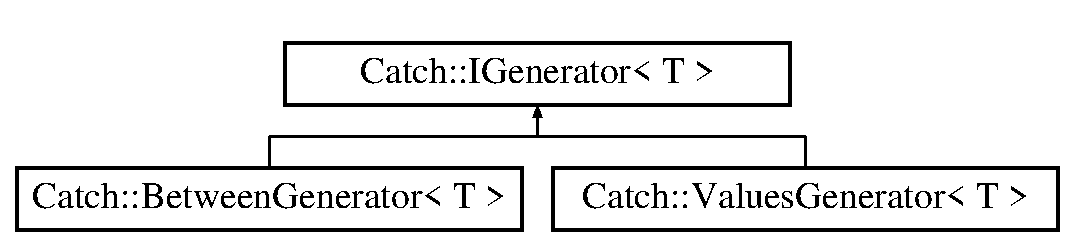
\includegraphics[height=2.000000cm]{structCatch_1_1IGenerator}
\end{center}
\end{figure}
\subsection*{Public Member Functions}
\begin{DoxyCompactItemize}
\item 
\mbox{\Hypertarget{structCatch_1_1IGenerator_ad69e937cb66dba3ed9429c42abf4fce3}\label{structCatch_1_1IGenerator_ad69e937cb66dba3ed9429c42abf4fce3}} 
virtual T {\bfseries get\+Value} (std\+::size\+\_\+t index) const =0
\item 
\mbox{\Hypertarget{structCatch_1_1IGenerator_a2e317253b03e838b6065ce69719a198e}\label{structCatch_1_1IGenerator_a2e317253b03e838b6065ce69719a198e}} 
virtual std\+::size\+\_\+t {\bfseries size} () const =0
\end{DoxyCompactItemize}


The documentation for this struct was generated from the following file\+:\begin{DoxyCompactItemize}
\item 
test\+\_\+cases/catch.\+hpp\end{DoxyCompactItemize}

\hypertarget{structCatch_1_1IGeneratorInfo}{}\section{Catch\+:\+:I\+Generator\+Info Struct Reference}
\label{structCatch_1_1IGeneratorInfo}\index{Catch\+::\+I\+Generator\+Info@{Catch\+::\+I\+Generator\+Info}}
\subsection*{Public Member Functions}
\begin{DoxyCompactItemize}
\item 
\mbox{\Hypertarget{structCatch_1_1IGeneratorInfo_a2b86711ca7009903edfe27ed62b515ef}\label{structCatch_1_1IGeneratorInfo_a2b86711ca7009903edfe27ed62b515ef}} 
virtual bool {\bfseries move\+Next} ()=0
\item 
\mbox{\Hypertarget{structCatch_1_1IGeneratorInfo_a6a0dca712d31f6849fd9447b1344673a}\label{structCatch_1_1IGeneratorInfo_a6a0dca712d31f6849fd9447b1344673a}} 
virtual std\+::size\+\_\+t {\bfseries get\+Current\+Index} () const =0
\end{DoxyCompactItemize}


The documentation for this struct was generated from the following file\+:\begin{DoxyCompactItemize}
\item 
test\+\_\+cases/catch.\+hpp\end{DoxyCompactItemize}

\hypertarget{structCatch_1_1IGeneratorsForTest}{}\section{Catch\+:\+:I\+Generators\+For\+Test Struct Reference}
\label{structCatch_1_1IGeneratorsForTest}\index{Catch\+::\+I\+Generators\+For\+Test@{Catch\+::\+I\+Generators\+For\+Test}}
\subsection*{Public Member Functions}
\begin{DoxyCompactItemize}
\item 
\mbox{\Hypertarget{structCatch_1_1IGeneratorsForTest_a180d84e858840188e4c3788e47eefdb0}\label{structCatch_1_1IGeneratorsForTest_a180d84e858840188e4c3788e47eefdb0}} 
virtual \hyperlink{structCatch_1_1IGeneratorInfo}{I\+Generator\+Info} \& {\bfseries get\+Generator\+Info} (std\+::string const \&file\+Info, std\+::size\+\_\+t size)=0
\item 
\mbox{\Hypertarget{structCatch_1_1IGeneratorsForTest_adab31832d529fc584fd63164e0a1c8ad}\label{structCatch_1_1IGeneratorsForTest_adab31832d529fc584fd63164e0a1c8ad}} 
virtual bool {\bfseries move\+Next} ()=0
\end{DoxyCompactItemize}


The documentation for this struct was generated from the following file\+:\begin{DoxyCompactItemize}
\item 
test\+\_\+cases/catch.\+hpp\end{DoxyCompactItemize}

\hypertarget{classImmediateInstructionModifier}{}\section{Immediate\+Instruction\+Modifier Class Reference}
\label{classImmediateInstructionModifier}\index{Immediate\+Instruction\+Modifier@{Immediate\+Instruction\+Modifier}}
Inheritance diagram for Immediate\+Instruction\+Modifier\+:\begin{figure}[H]
\begin{center}
\leavevmode
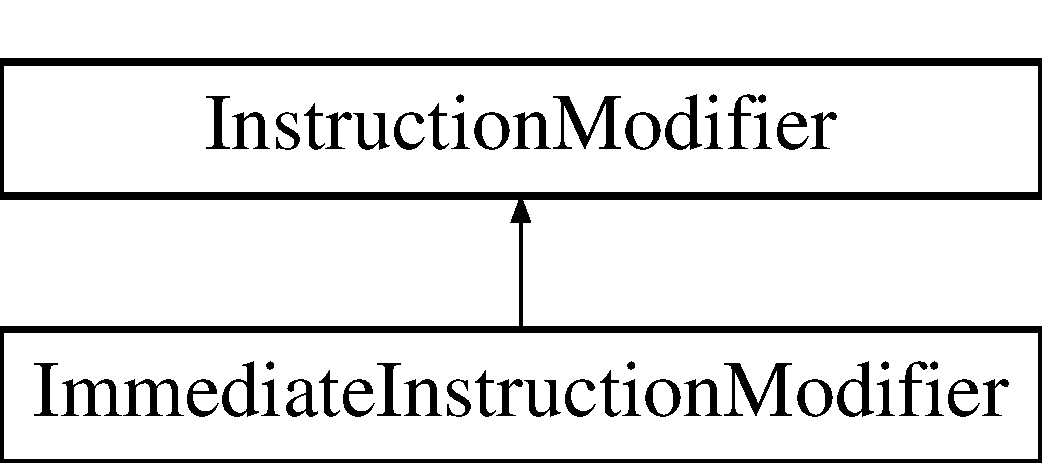
\includegraphics[height=2.000000cm]{classImmediateInstructionModifier}
\end{center}
\end{figure}
\subsection*{Public Member Functions}
\begin{DoxyCompactItemize}
\item 
\mbox{\Hypertarget{classImmediateInstructionModifier_aa7e056831824684e06dfa6b1c573272a}\label{classImmediateInstructionModifier_aa7e056831824684e06dfa6b1c573272a}} 
std\+::shared\+\_\+ptr$<$ \hyperlink{classInstructionModifier}{Instruction\+Modifier} $>$ {\bfseries clone} () const override
\item 
\mbox{\Hypertarget{classImmediateInstructionModifier_a5fd1e82bd9300c68f0f4afe196602185}\label{classImmediateInstructionModifier_a5fd1e82bd9300c68f0f4afe196602185}} 
{\bfseries Immediate\+Instruction\+Modifier} (const char modifier\+Code)
\item 
\mbox{\Hypertarget{classImmediateInstructionModifier_a7d9f20931dad071a78c925df789c4972}\label{classImmediateInstructionModifier_a7d9f20931dad071a78c925df789c4972}} 
boost\+::optional$<$ \hyperlink{classInstruction}{Instruction} $>$ {\bfseries find\+Target\+Instruction} (\hyperlink{classMemoryIndex}{Memory\+Index} \&m\+Index, const std\+::vector$<$ \hyperlink{classInstruction}{Instruction} $>$ memory\+Array) override
\end{DoxyCompactItemize}


The documentation for this class was generated from the following files\+:\begin{DoxyCompactItemize}
\item 
logic/parser/Immediate\+Instruction\+Modifier.\+h\item 
logic/parser/Immediate\+Instruction\+Modifier.\+cpp\end{DoxyCompactItemize}

\hypertarget{structCatch_1_1IMutableContext}{}\section{Catch\+:\+:I\+Mutable\+Context Struct Reference}
\label{structCatch_1_1IMutableContext}\index{Catch\+::\+I\+Mutable\+Context@{Catch\+::\+I\+Mutable\+Context}}
Inheritance diagram for Catch\+:\+:I\+Mutable\+Context\+:\begin{figure}[H]
\begin{center}
\leavevmode
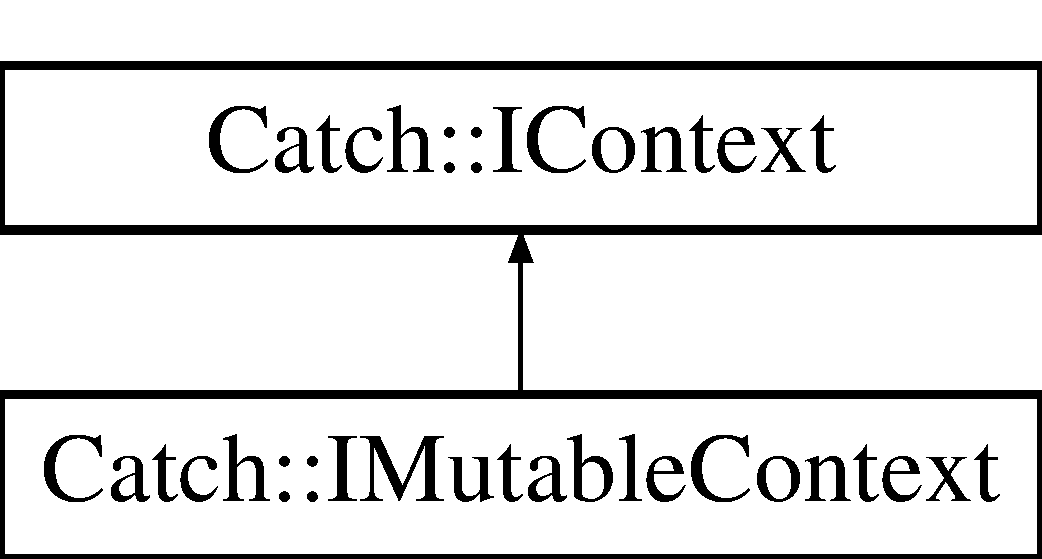
\includegraphics[height=2.000000cm]{structCatch_1_1IMutableContext}
\end{center}
\end{figure}
\subsection*{Public Member Functions}
\begin{DoxyCompactItemize}
\item 
\mbox{\Hypertarget{structCatch_1_1IMutableContext_a4a80afd0525b7def21bee8d9b48f2d39}\label{structCatch_1_1IMutableContext_a4a80afd0525b7def21bee8d9b48f2d39}} 
virtual void {\bfseries set\+Result\+Capture} (\hyperlink{structCatch_1_1IResultCapture}{I\+Result\+Capture} $\ast$result\+Capture)=0
\item 
\mbox{\Hypertarget{structCatch_1_1IMutableContext_af2e53b1dea4527a2587cff266a730f6e}\label{structCatch_1_1IMutableContext_af2e53b1dea4527a2587cff266a730f6e}} 
virtual void {\bfseries set\+Runner} (\hyperlink{structCatch_1_1IRunner}{I\+Runner} $\ast$runner)=0
\item 
\mbox{\Hypertarget{structCatch_1_1IMutableContext_a013e8f688a8ea7970262d07ead542a63}\label{structCatch_1_1IMutableContext_a013e8f688a8ea7970262d07ead542a63}} 
virtual void {\bfseries set\+Config} (\hyperlink{classCatch_1_1Ptr}{Ptr}$<$ I\+Config const $>$ const \&config)=0
\end{DoxyCompactItemize}


The documentation for this struct was generated from the following file\+:\begin{DoxyCompactItemize}
\item 
test\+\_\+cases/catch.\+hpp\end{DoxyCompactItemize}

\hypertarget{structCatch_1_1IMutableRegistryHub}{}\section{Catch\+:\+:I\+Mutable\+Registry\+Hub Struct Reference}
\label{structCatch_1_1IMutableRegistryHub}\index{Catch\+::\+I\+Mutable\+Registry\+Hub@{Catch\+::\+I\+Mutable\+Registry\+Hub}}
\subsection*{Public Member Functions}
\begin{DoxyCompactItemize}
\item 
\mbox{\Hypertarget{structCatch_1_1IMutableRegistryHub_aab72d0aa1fa14627f1a6a4c893ae0a12}\label{structCatch_1_1IMutableRegistryHub_aab72d0aa1fa14627f1a6a4c893ae0a12}} 
virtual void {\bfseries register\+Reporter} (std\+::string const \&name, \hyperlink{classCatch_1_1Ptr}{Ptr}$<$ I\+Reporter\+Factory $>$ const \&factory)=0
\item 
\mbox{\Hypertarget{structCatch_1_1IMutableRegistryHub_ae06fcb90ba3f2b389d450cd81e229276}\label{structCatch_1_1IMutableRegistryHub_ae06fcb90ba3f2b389d450cd81e229276}} 
virtual void {\bfseries register\+Listener} (\hyperlink{classCatch_1_1Ptr}{Ptr}$<$ I\+Reporter\+Factory $>$ const \&factory)=0
\item 
\mbox{\Hypertarget{structCatch_1_1IMutableRegistryHub_a11b85c6744d88c9f83fe16ad4a8dd451}\label{structCatch_1_1IMutableRegistryHub_a11b85c6744d88c9f83fe16ad4a8dd451}} 
virtual void {\bfseries register\+Test} (\hyperlink{classCatch_1_1TestCase}{Test\+Case} const \&test\+Info)=0
\item 
\mbox{\Hypertarget{structCatch_1_1IMutableRegistryHub_ae6825365102693cf7707db022a2c2b49}\label{structCatch_1_1IMutableRegistryHub_ae6825365102693cf7707db022a2c2b49}} 
virtual void {\bfseries register\+Translator} (const \hyperlink{structCatch_1_1IExceptionTranslator}{I\+Exception\+Translator} $\ast$translator)=0
\item 
\mbox{\Hypertarget{structCatch_1_1IMutableRegistryHub_abf2e386b6f94f615719ada711adbf822}\label{structCatch_1_1IMutableRegistryHub_abf2e386b6f94f615719ada711adbf822}} 
virtual void {\bfseries register\+Tag\+Alias} (std\+::string const \&alias, std\+::string const \&tag, \hyperlink{structCatch_1_1SourceLineInfo}{Source\+Line\+Info} const \&line\+Info)=0
\end{DoxyCompactItemize}


The documentation for this struct was generated from the following file\+:\begin{DoxyCompactItemize}
\item 
test\+\_\+cases/catch.\+hpp\end{DoxyCompactItemize}

\hypertarget{classIndirectInstructionModifier}{}\section{Indirect\+Instruction\+Modifier Class Reference}
\label{classIndirectInstructionModifier}\index{Indirect\+Instruction\+Modifier@{Indirect\+Instruction\+Modifier}}
Inheritance diagram for Indirect\+Instruction\+Modifier\+:\begin{figure}[H]
\begin{center}
\leavevmode
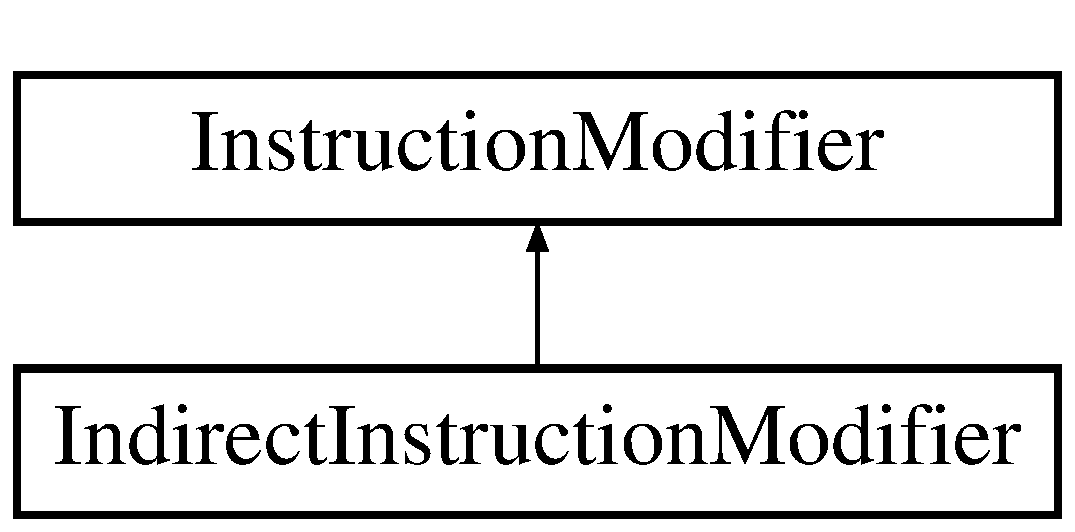
\includegraphics[height=2.000000cm]{classIndirectInstructionModifier}
\end{center}
\end{figure}
\subsection*{Public Member Functions}
\begin{DoxyCompactItemize}
\item 
\mbox{\Hypertarget{classIndirectInstructionModifier_adea8e4cec4a4c02c2144663ce6acd6d3}\label{classIndirectInstructionModifier_adea8e4cec4a4c02c2144663ce6acd6d3}} 
std\+::shared\+\_\+ptr$<$ \hyperlink{classInstructionModifier}{Instruction\+Modifier} $>$ {\bfseries clone} () const override
\item 
\mbox{\Hypertarget{classIndirectInstructionModifier_a4ff00cbee335058a785365c014cc4aff}\label{classIndirectInstructionModifier_a4ff00cbee335058a785365c014cc4aff}} 
boost\+::optional$<$ \hyperlink{classInstruction}{Instruction} $>$ {\bfseries find\+Target\+Instruction} (\hyperlink{classMemoryIndex}{Memory\+Index} \&m\+Index, const std\+::vector$<$ \hyperlink{classInstruction}{Instruction} $>$ memory\+Array) override
\end{DoxyCompactItemize}


The documentation for this class was generated from the following files\+:\begin{DoxyCompactItemize}
\item 
logic/parser/Indirect\+Instruction\+Modifier.\+h\item 
logic/parser/Indirect\+Instruction\+Modifier.\+cpp\end{DoxyCompactItemize}

\hypertarget{classInitializer}{}\section{Initializer Class Reference}
\label{classInitializer}\index{Initializer@{Initializer}}
\subsection*{Public Member Functions}
\begin{DoxyCompactItemize}
\item 
vector$<$ \hyperlink{classInstruction}{Instruction} $>$ \hyperlink{classInitializer_a3bca75fbbca3beafebcc234b4749bdb5}{send\+Code\+Request\+And\+Parse} ()
\end{DoxyCompactItemize}


\subsection{Member Function Documentation}
\mbox{\Hypertarget{classInitializer_a3bca75fbbca3beafebcc234b4749bdb5}\label{classInitializer_a3bca75fbbca3beafebcc234b4749bdb5}} 
\index{Initializer@{Initializer}!send\+Code\+Request\+And\+Parse@{send\+Code\+Request\+And\+Parse}}
\index{send\+Code\+Request\+And\+Parse@{send\+Code\+Request\+And\+Parse}!Initializer@{Initializer}}
\subsubsection{\texorpdfstring{send\+Code\+Request\+And\+Parse()}{sendCodeRequestAndParse()}}
{\footnotesize\ttfamily vector$<$ \hyperlink{classInstruction}{Instruction} $>$ Initializer\+::send\+Code\+Request\+And\+Parse (\begin{DoxyParamCaption}{ }\end{DoxyParamCaption})}

asks for warrior code and parses it \begin{DoxyReturn}{Returns}
vector of Redcode instructions parsed from warrior code 
\end{DoxyReturn}


The documentation for this class was generated from the following files\+:\begin{DoxyCompactItemize}
\item 
logic/Initializer.\+h\item 
logic/Initializer.\+cpp\end{DoxyCompactItemize}

\hypertarget{classInstruction}{}\section{Instruction Class Reference}
\label{classInstruction}\index{Instruction@{Instruction}}


{\ttfamily \#include $<$Instruction.\+h$>$}

\subsection*{Public Member Functions}
\begin{DoxyCompactItemize}
\item 
\hyperlink{classInstruction_a8189c6e3e0caeaec698ae8053abf84b4}{Instruction} (const std\+::shared\+\_\+ptr$<$ \hyperlink{classInstructionModifier}{Instruction\+Modifier} $>$ operatorA, const std\+::shared\+\_\+ptr$<$ \hyperlink{classInstructionModifier}{Instruction\+Modifier} $>$ operatorB)
\item 
\hyperlink{classInstruction_ad1758d4d7afbf358e529e1ce5b199890}{Instruction} (const std\+::shared\+\_\+ptr$<$ \hyperlink{classMarsOperation}{Mars\+Operation} $>$ operation)
\item 
\hyperlink{classInstruction_a89efff676fc87ab4f831f4e7f4d574b9}{Instruction} (const std\+::shared\+\_\+ptr$<$ \hyperlink{classMarsOperation}{Mars\+Operation} $>$ operation, const std\+::shared\+\_\+ptr$<$ \hyperlink{classInstructionModifier}{Instruction\+Modifier} $>$ operatorA, const std\+::shared\+\_\+ptr$<$ \hyperlink{classInstructionModifier}{Instruction\+Modifier} $>$ operatorB)
\item 
const std\+::shared\+\_\+ptr$<$ \hyperlink{classMarsOperation}{Mars\+Operation} $>$ \& \hyperlink{classInstruction_a2cff68de6bb0e59aa8d32adb7c5a956a}{get\+Operation} () const
\item 
void \hyperlink{classInstruction_a6c3579495382c92ec38816636d2e98ef}{set\+Operation} (const std\+::shared\+\_\+ptr$<$ \hyperlink{classMarsOperation}{Mars\+Operation} $>$ \&operation)
\item 
const std\+::shared\+\_\+ptr$<$ \hyperlink{classInstructionModifier}{Instruction\+Modifier} $>$ \& \hyperlink{classInstruction_a2a21f6752465fd7d3401d43d57b7fa83}{get\+AddressA} () const
\item 
void \hyperlink{classInstruction_a3d0eeea6b5824a82518383e282550a39}{set\+AddressA} (const std\+::shared\+\_\+ptr$<$ \hyperlink{classInstructionModifier}{Instruction\+Modifier} $>$ \&addressA)
\item 
const std\+::shared\+\_\+ptr$<$ \hyperlink{classInstructionModifier}{Instruction\+Modifier} $>$ \& \hyperlink{classInstruction_a587656e972cb049fe5cd22159451d508}{get\+AddressB} () const
\item 
void \hyperlink{classInstruction_a8537c5d0dd3696b5f48ae297f4e89dbf}{set\+AddressB} (const std\+::shared\+\_\+ptr$<$ \hyperlink{classInstructionModifier}{Instruction\+Modifier} $>$ \&addressB)
\item 
void \hyperlink{classInstruction_a69c97b99c08ae8997122fb99e139c9aa}{add\+To\+A\+Value} (int i)
\item 
void \hyperlink{classInstruction_af626c46ca16688de0a7b31a88817fd39}{add\+To\+B\+Value} (int i)
\item 
int \hyperlink{classInstruction_a86228a629fcccffffeb73b9b17201864}{get\+A\+Value} ()
\item 
int \hyperlink{classInstruction_a02e899031bb2cb33d6e09bcfce3f9569}{get\+B\+Value} ()
\item 
void \hyperlink{classInstruction_a3650c10f4821a87e865906c5095d9e98}{set\+A\+Value} (int i)
\item 
void \hyperlink{classInstruction_aff4dda9270970f00f48d70245a79122c}{set\+B\+Value} (int i)
\end{DoxyCompactItemize}


\subsection{Detailed Description}
Base class representing \hyperlink{classInstruction}{Instruction}. A single \hyperlink{classInstruction}{Instruction} consists of 2 operators and an operation 

\subsection{Constructor \& Destructor Documentation}
\mbox{\Hypertarget{classInstruction_a8189c6e3e0caeaec698ae8053abf84b4}\label{classInstruction_a8189c6e3e0caeaec698ae8053abf84b4}} 
\index{Instruction@{Instruction}!Instruction@{Instruction}}
\index{Instruction@{Instruction}!Instruction@{Instruction}}
\subsubsection{\texorpdfstring{Instruction()}{Instruction()}\hspace{0.1cm}{\footnotesize\ttfamily [1/3]}}
{\footnotesize\ttfamily Instruction\+::\+Instruction (\begin{DoxyParamCaption}\item[{const std\+::shared\+\_\+ptr$<$ \hyperlink{classInstructionModifier}{Instruction\+Modifier} $>$}]{operatorA,  }\item[{const std\+::shared\+\_\+ptr$<$ \hyperlink{classInstructionModifier}{Instruction\+Modifier} $>$}]{operatorB }\end{DoxyParamCaption})}

Constructor without specified operation 
\begin{DoxyParams}{Parameters}
{\em operatorA} & first address \\
\hline
{\em operatorB} & second address \\
\hline
\end{DoxyParams}
\mbox{\Hypertarget{classInstruction_ad1758d4d7afbf358e529e1ce5b199890}\label{classInstruction_ad1758d4d7afbf358e529e1ce5b199890}} 
\index{Instruction@{Instruction}!Instruction@{Instruction}}
\index{Instruction@{Instruction}!Instruction@{Instruction}}
\subsubsection{\texorpdfstring{Instruction()}{Instruction()}\hspace{0.1cm}{\footnotesize\ttfamily [2/3]}}
{\footnotesize\ttfamily Instruction\+::\+Instruction (\begin{DoxyParamCaption}\item[{const std\+::shared\+\_\+ptr$<$ \hyperlink{classMarsOperation}{Mars\+Operation} $>$}]{operation }\end{DoxyParamCaption})}

Constructor without specified operators 
\begin{DoxyParams}{Parameters}
{\em operation} & Operation \\
\hline
\end{DoxyParams}
\mbox{\Hypertarget{classInstruction_a89efff676fc87ab4f831f4e7f4d574b9}\label{classInstruction_a89efff676fc87ab4f831f4e7f4d574b9}} 
\index{Instruction@{Instruction}!Instruction@{Instruction}}
\index{Instruction@{Instruction}!Instruction@{Instruction}}
\subsubsection{\texorpdfstring{Instruction()}{Instruction()}\hspace{0.1cm}{\footnotesize\ttfamily [3/3]}}
{\footnotesize\ttfamily Instruction\+::\+Instruction (\begin{DoxyParamCaption}\item[{const std\+::shared\+\_\+ptr$<$ \hyperlink{classMarsOperation}{Mars\+Operation} $>$}]{operation,  }\item[{const std\+::shared\+\_\+ptr$<$ \hyperlink{classInstructionModifier}{Instruction\+Modifier} $>$}]{operatorA,  }\item[{const std\+::shared\+\_\+ptr$<$ \hyperlink{classInstructionModifier}{Instruction\+Modifier} $>$}]{operatorB }\end{DoxyParamCaption})}

Constructor 
\begin{DoxyParams}{Parameters}
{\em operation} & Operation \\
\hline
{\em operatorA} & First address \\
\hline
{\em operatorB} & Second address \\
\hline
\end{DoxyParams}


\subsection{Member Function Documentation}
\mbox{\Hypertarget{classInstruction_a69c97b99c08ae8997122fb99e139c9aa}\label{classInstruction_a69c97b99c08ae8997122fb99e139c9aa}} 
\index{Instruction@{Instruction}!add\+To\+A\+Value@{add\+To\+A\+Value}}
\index{add\+To\+A\+Value@{add\+To\+A\+Value}!Instruction@{Instruction}}
\subsubsection{\texorpdfstring{add\+To\+A\+Value()}{addToAValue()}}
{\footnotesize\ttfamily void Instruction\+::add\+To\+A\+Value (\begin{DoxyParamCaption}\item[{int}]{i }\end{DoxyParamCaption})}

Adds i to addressA 
\begin{DoxyParams}{Parameters}
{\em i} & value to add \\
\hline
\end{DoxyParams}
\mbox{\Hypertarget{classInstruction_af626c46ca16688de0a7b31a88817fd39}\label{classInstruction_af626c46ca16688de0a7b31a88817fd39}} 
\index{Instruction@{Instruction}!add\+To\+B\+Value@{add\+To\+B\+Value}}
\index{add\+To\+B\+Value@{add\+To\+B\+Value}!Instruction@{Instruction}}
\subsubsection{\texorpdfstring{add\+To\+B\+Value()}{addToBValue()}}
{\footnotesize\ttfamily void Instruction\+::add\+To\+B\+Value (\begin{DoxyParamCaption}\item[{int}]{i }\end{DoxyParamCaption})}

Adds i to addressB 
\begin{DoxyParams}{Parameters}
{\em i} & value to add \\
\hline
\end{DoxyParams}
\mbox{\Hypertarget{classInstruction_a2a21f6752465fd7d3401d43d57b7fa83}\label{classInstruction_a2a21f6752465fd7d3401d43d57b7fa83}} 
\index{Instruction@{Instruction}!get\+AddressA@{get\+AddressA}}
\index{get\+AddressA@{get\+AddressA}!Instruction@{Instruction}}
\subsubsection{\texorpdfstring{get\+Address\+A()}{getAddressA()}}
{\footnotesize\ttfamily const std\+::shared\+\_\+ptr$<$ \hyperlink{classInstructionModifier}{Instruction\+Modifier} $>$ \& Instruction\+::get\+AddressA (\begin{DoxyParamCaption}{ }\end{DoxyParamCaption}) const}

Returns first address \begin{DoxyReturn}{Returns}
addressA 
\end{DoxyReturn}
\mbox{\Hypertarget{classInstruction_a587656e972cb049fe5cd22159451d508}\label{classInstruction_a587656e972cb049fe5cd22159451d508}} 
\index{Instruction@{Instruction}!get\+AddressB@{get\+AddressB}}
\index{get\+AddressB@{get\+AddressB}!Instruction@{Instruction}}
\subsubsection{\texorpdfstring{get\+Address\+B()}{getAddressB()}}
{\footnotesize\ttfamily const std\+::shared\+\_\+ptr$<$ \hyperlink{classInstructionModifier}{Instruction\+Modifier} $>$ \& Instruction\+::get\+AddressB (\begin{DoxyParamCaption}{ }\end{DoxyParamCaption}) const}

Returns second address \begin{DoxyReturn}{Returns}
addressB 
\end{DoxyReturn}
\mbox{\Hypertarget{classInstruction_a86228a629fcccffffeb73b9b17201864}\label{classInstruction_a86228a629fcccffffeb73b9b17201864}} 
\index{Instruction@{Instruction}!get\+A\+Value@{get\+A\+Value}}
\index{get\+A\+Value@{get\+A\+Value}!Instruction@{Instruction}}
\subsubsection{\texorpdfstring{get\+A\+Value()}{getAValue()}}
{\footnotesize\ttfamily int Instruction\+::get\+A\+Value (\begin{DoxyParamCaption}{ }\end{DoxyParamCaption})}

Returns value of first address \begin{DoxyReturn}{Returns}
value of first address 
\end{DoxyReturn}
\mbox{\Hypertarget{classInstruction_a02e899031bb2cb33d6e09bcfce3f9569}\label{classInstruction_a02e899031bb2cb33d6e09bcfce3f9569}} 
\index{Instruction@{Instruction}!get\+B\+Value@{get\+B\+Value}}
\index{get\+B\+Value@{get\+B\+Value}!Instruction@{Instruction}}
\subsubsection{\texorpdfstring{get\+B\+Value()}{getBValue()}}
{\footnotesize\ttfamily int Instruction\+::get\+B\+Value (\begin{DoxyParamCaption}{ }\end{DoxyParamCaption})}

Returns value of second address \begin{DoxyReturn}{Returns}
value of second address 
\end{DoxyReturn}
\mbox{\Hypertarget{classInstruction_a2cff68de6bb0e59aa8d32adb7c5a956a}\label{classInstruction_a2cff68de6bb0e59aa8d32adb7c5a956a}} 
\index{Instruction@{Instruction}!get\+Operation@{get\+Operation}}
\index{get\+Operation@{get\+Operation}!Instruction@{Instruction}}
\subsubsection{\texorpdfstring{get\+Operation()}{getOperation()}}
{\footnotesize\ttfamily const std\+::shared\+\_\+ptr$<$ \hyperlink{classMarsOperation}{Mars\+Operation} $>$ \& Instruction\+::get\+Operation (\begin{DoxyParamCaption}{ }\end{DoxyParamCaption}) const}

Returns operation \begin{DoxyReturn}{Returns}
operation 
\end{DoxyReturn}
\mbox{\Hypertarget{classInstruction_a3d0eeea6b5824a82518383e282550a39}\label{classInstruction_a3d0eeea6b5824a82518383e282550a39}} 
\index{Instruction@{Instruction}!set\+AddressA@{set\+AddressA}}
\index{set\+AddressA@{set\+AddressA}!Instruction@{Instruction}}
\subsubsection{\texorpdfstring{set\+Address\+A()}{setAddressA()}}
{\footnotesize\ttfamily void Instruction\+::set\+AddressA (\begin{DoxyParamCaption}\item[{const std\+::shared\+\_\+ptr$<$ \hyperlink{classInstructionModifier}{Instruction\+Modifier} $>$ \&}]{addressA }\end{DoxyParamCaption})}

Sets first address 
\begin{DoxyParams}{Parameters}
{\em addressA} & First address \\
\hline
\end{DoxyParams}
\mbox{\Hypertarget{classInstruction_a8537c5d0dd3696b5f48ae297f4e89dbf}\label{classInstruction_a8537c5d0dd3696b5f48ae297f4e89dbf}} 
\index{Instruction@{Instruction}!set\+AddressB@{set\+AddressB}}
\index{set\+AddressB@{set\+AddressB}!Instruction@{Instruction}}
\subsubsection{\texorpdfstring{set\+Address\+B()}{setAddressB()}}
{\footnotesize\ttfamily void Instruction\+::set\+AddressB (\begin{DoxyParamCaption}\item[{const std\+::shared\+\_\+ptr$<$ \hyperlink{classInstructionModifier}{Instruction\+Modifier} $>$ \&}]{addressB }\end{DoxyParamCaption})}

Sets second address 
\begin{DoxyParams}{Parameters}
{\em addressA} & Second address \\
\hline
\end{DoxyParams}
\mbox{\Hypertarget{classInstruction_a3650c10f4821a87e865906c5095d9e98}\label{classInstruction_a3650c10f4821a87e865906c5095d9e98}} 
\index{Instruction@{Instruction}!set\+A\+Value@{set\+A\+Value}}
\index{set\+A\+Value@{set\+A\+Value}!Instruction@{Instruction}}
\subsubsection{\texorpdfstring{set\+A\+Value()}{setAValue()}}
{\footnotesize\ttfamily void Instruction\+::set\+A\+Value (\begin{DoxyParamCaption}\item[{int}]{i }\end{DoxyParamCaption})}

Sets value of first address 
\begin{DoxyParams}{Parameters}
{\em i} & new value of first address \\
\hline
\end{DoxyParams}
\mbox{\Hypertarget{classInstruction_aff4dda9270970f00f48d70245a79122c}\label{classInstruction_aff4dda9270970f00f48d70245a79122c}} 
\index{Instruction@{Instruction}!set\+B\+Value@{set\+B\+Value}}
\index{set\+B\+Value@{set\+B\+Value}!Instruction@{Instruction}}
\subsubsection{\texorpdfstring{set\+B\+Value()}{setBValue()}}
{\footnotesize\ttfamily void Instruction\+::set\+B\+Value (\begin{DoxyParamCaption}\item[{int}]{i }\end{DoxyParamCaption})}

Sets value of second address 
\begin{DoxyParams}{Parameters}
{\em i} & new value of second address \\
\hline
\end{DoxyParams}
\mbox{\Hypertarget{classInstruction_a6c3579495382c92ec38816636d2e98ef}\label{classInstruction_a6c3579495382c92ec38816636d2e98ef}} 
\index{Instruction@{Instruction}!set\+Operation@{set\+Operation}}
\index{set\+Operation@{set\+Operation}!Instruction@{Instruction}}
\subsubsection{\texorpdfstring{set\+Operation()}{setOperation()}}
{\footnotesize\ttfamily void Instruction\+::set\+Operation (\begin{DoxyParamCaption}\item[{const std\+::shared\+\_\+ptr$<$ \hyperlink{classMarsOperation}{Mars\+Operation} $>$ \&}]{operation }\end{DoxyParamCaption})}

Sets operation 
\begin{DoxyParams}{Parameters}
{\em operation} & \\
\hline
\end{DoxyParams}


The documentation for this class was generated from the following files\+:\begin{DoxyCompactItemize}
\item 
logic/mars/Instruction.\+h\item 
logic/mars/Instruction.\+cpp\end{DoxyCompactItemize}

\hypertarget{classInstructionCreator}{}\section{Instruction\+Creator Class Reference}
\label{classInstructionCreator}\index{Instruction\+Creator@{Instruction\+Creator}}
\subsection*{Static Public Member Functions}
\begin{DoxyCompactItemize}
\item 
\mbox{\Hypertarget{classInstructionCreator_aff6cd584032ef7dc4b7f4b1d2dedda39}\label{classInstructionCreator_aff6cd584032ef7dc4b7f4b1d2dedda39}} 
static \hyperlink{classInstruction}{Instruction} {\bfseries try\+Create} (\hyperlink{classInstructionData}{Instruction\+Data} data)
\item 
\mbox{\Hypertarget{classInstructionCreator_a6075f2a2e077f186f115ee911bf53169}\label{classInstructionCreator_a6075f2a2e077f186f115ee911bf53169}} 
static \hyperlink{classInstruction}{Instruction} {\bfseries create\+Default} ()
\end{DoxyCompactItemize}


The documentation for this class was generated from the following files\+:\begin{DoxyCompactItemize}
\item 
logic/parser/Instruction\+Creator.\+h\item 
logic/parser/Instruction\+Creator.\+cpp\end{DoxyCompactItemize}

\hypertarget{classInstructionData}{}\section{Instruction\+Data Class Reference}
\label{classInstructionData}\index{Instruction\+Data@{Instruction\+Data}}
\subsection*{Public Member Functions}
\begin{DoxyCompactItemize}
\item 
\mbox{\Hypertarget{classInstructionData_aca4d7e3e5ee2d317daa11eecb9e3b80b}\label{classInstructionData_aca4d7e3e5ee2d317daa11eecb9e3b80b}} 
{\bfseries Instruction\+Data} (const string \&code, const string \&a\+\_\+field, const string \&b\+\_\+field)
\item 
\mbox{\Hypertarget{classInstructionData_a24df36f2815df009ab28f415a03e2df5}\label{classInstructionData_a24df36f2815df009ab28f415a03e2df5}} 
const string \& {\bfseries get\+Code} () const
\item 
\mbox{\Hypertarget{classInstructionData_a2cfad65ce30b28785d7c0a01822677ec}\label{classInstructionData_a2cfad65ce30b28785d7c0a01822677ec}} 
void {\bfseries set\+Code} (const string \&code)
\item 
\mbox{\Hypertarget{classInstructionData_aee6171141ba4998760bad4db6c101c47}\label{classInstructionData_aee6171141ba4998760bad4db6c101c47}} 
const string \& {\bfseries get\+A\+\_\+field} () const
\item 
\mbox{\Hypertarget{classInstructionData_ab71eb04ab2e46502c3f981443e12ed39}\label{classInstructionData_ab71eb04ab2e46502c3f981443e12ed39}} 
void {\bfseries set\+A\+\_\+field} (const string \&a\+\_\+field)
\item 
\mbox{\Hypertarget{classInstructionData_a569cf018c8f6b90b2c91ac03f0522820}\label{classInstructionData_a569cf018c8f6b90b2c91ac03f0522820}} 
const string \& {\bfseries get\+B\+\_\+field} () const
\item 
\mbox{\Hypertarget{classInstructionData_ab941a4d2566cc2fdfe7265ea9e4f5f93}\label{classInstructionData_ab941a4d2566cc2fdfe7265ea9e4f5f93}} 
void {\bfseries set\+B\+\_\+field} (const string \&b\+\_\+field)
\end{DoxyCompactItemize}


The documentation for this class was generated from the following files\+:\begin{DoxyCompactItemize}
\item 
logic/parser/Instruction\+Data.\+h\item 
logic/parser/Instruction\+Data.\+cpp\end{DoxyCompactItemize}

\hypertarget{classInstructionDataExtractor}{}\section{Instruction\+Data\+Extractor Class Reference}
\label{classInstructionDataExtractor}\index{Instruction\+Data\+Extractor@{Instruction\+Data\+Extractor}}
\subsection*{Public Member Functions}
\begin{DoxyCompactItemize}
\item 
\mbox{\Hypertarget{classInstructionDataExtractor_a82bf23dcb5d0204a28745baee314d893}\label{classInstructionDataExtractor_a82bf23dcb5d0204a28745baee314d893}} 
\hyperlink{classInstructionData}{Instruction\+Data} {\bfseries try\+Extract} (std\+::string raw\+Instr)
\item 
\mbox{\Hypertarget{classInstructionDataExtractor_ad6f18216556a97b60018d4af6c5e8d8f}\label{classInstructionDataExtractor_ad6f18216556a97b60018d4af6c5e8d8f}} 
bool {\bfseries is\+Instruction\+Valid} (std\+::string raw\+Instr)
\end{DoxyCompactItemize}


The documentation for this class was generated from the following files\+:\begin{DoxyCompactItemize}
\item 
logic/parser/Instruction\+Data\+Extractor.\+h\item 
logic/parser/Instruction\+Data\+Extractor.\+cpp\end{DoxyCompactItemize}

\hypertarget{classInstructionModifier}{}\section{Instruction\+Modifier Class Reference}
\label{classInstructionModifier}\index{Instruction\+Modifier@{Instruction\+Modifier}}
Inheritance diagram for Instruction\+Modifier\+:\begin{figure}[H]
\begin{center}
\leavevmode
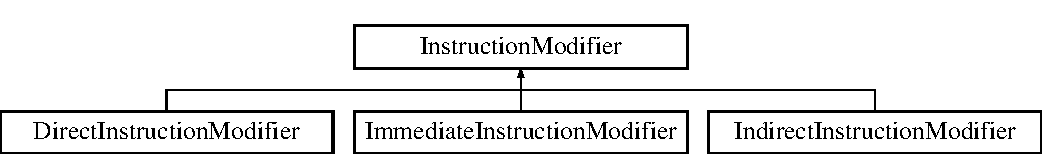
\includegraphics[height=2.000000cm]{classInstructionModifier}
\end{center}
\end{figure}
\subsection*{Public Member Functions}
\begin{DoxyCompactItemize}
\item 
\mbox{\Hypertarget{classInstructionModifier_a5df9e76d602aef4ddea650fbded1a87b}\label{classInstructionModifier_a5df9e76d602aef4ddea650fbded1a87b}} 
{\bfseries Instruction\+Modifier} (const std\+::string \&modifier\+Code, int value=0)
\item 
\mbox{\Hypertarget{classInstructionModifier_a9428b66e9cef33e36a23c29a560633b5}\label{classInstructionModifier_a9428b66e9cef33e36a23c29a560633b5}} 
virtual std\+::shared\+\_\+ptr$<$ \hyperlink{classInstructionModifier}{Instruction\+Modifier} $>$ {\bfseries clone} () const =0
\item 
\mbox{\Hypertarget{classInstructionModifier_a895656f8ed78b2556191e619fb8df5f1}\label{classInstructionModifier_a895656f8ed78b2556191e619fb8df5f1}} 
const std\+::string \& {\bfseries get\+Modifier\+Code} () const
\item 
\mbox{\Hypertarget{classInstructionModifier_a645afded73fb907e64720b1c9b53779e}\label{classInstructionModifier_a645afded73fb907e64720b1c9b53779e}} 
int {\bfseries get\+Value} () const
\item 
\mbox{\Hypertarget{classInstructionModifier_ad5bc86617da41a50fc17fd2c9c306800}\label{classInstructionModifier_ad5bc86617da41a50fc17fd2c9c306800}} 
void {\bfseries set\+Value} (int value)
\item 
\mbox{\Hypertarget{classInstructionModifier_ae2e69b35ffdb18e71c9c9716c57a7e31}\label{classInstructionModifier_ae2e69b35ffdb18e71c9c9716c57a7e31}} 
void {\bfseries set\+Modifier\+Code} (const std\+::string \&modifier\+Code)
\item 
\mbox{\Hypertarget{classInstructionModifier_a92b1272c5bce16b9d6a04841a6ee35e1}\label{classInstructionModifier_a92b1272c5bce16b9d6a04841a6ee35e1}} 
virtual boost\+::optional$<$ \hyperlink{classInstruction}{Instruction} $>$ {\bfseries find\+Target\+Instruction} (\hyperlink{classMemoryIndex}{Memory\+Index} \&m\+Index, const std\+::vector$<$ \hyperlink{classInstruction}{Instruction} $>$ memory\+Array)=0
\end{DoxyCompactItemize}


The documentation for this class was generated from the following files\+:\begin{DoxyCompactItemize}
\item 
logic/parser/Instruction\+Modifier.\+h\item 
logic/parser/Instruction\+Modifier.\+cpp\end{DoxyCompactItemize}

\hypertarget{classInstructionModifierCreator}{}\section{Instruction\+Modifier\+Creator Class Reference}
\label{classInstructionModifierCreator}\index{Instruction\+Modifier\+Creator@{Instruction\+Modifier\+Creator}}
\subsection*{Static Public Member Functions}
\begin{DoxyCompactItemize}
\item 
\mbox{\Hypertarget{classInstructionModifierCreator_aacc346f4ae622c29e8492dc093570dee}\label{classInstructionModifierCreator_aacc346f4ae622c29e8492dc093570dee}} 
static std\+::shared\+\_\+ptr$<$ \hyperlink{classInstructionModifier}{Instruction\+Modifier} $>$ {\bfseries try\+Create} (std\+::string)
\item 
\mbox{\Hypertarget{classInstructionModifierCreator_ae27a5b74da39fc74028db9c4efc01ad5}\label{classInstructionModifierCreator_ae27a5b74da39fc74028db9c4efc01ad5}} 
static int {\bfseries parse\+Address\+Value} (std\+::string num\+As\+String)
\item 
\mbox{\Hypertarget{classInstructionModifierCreator_a10376ec1982ca1a51d70251e6192390c}\label{classInstructionModifierCreator_a10376ec1982ca1a51d70251e6192390c}} 
static std\+::shared\+\_\+ptr$<$ \hyperlink{classInstructionModifier}{Instruction\+Modifier} $>$ {\bfseries create\+Default} ()
\end{DoxyCompactItemize}


The documentation for this class was generated from the following files\+:\begin{DoxyCompactItemize}
\item 
logic/parser/Instruction\+Modifier\+Creator.\+h\item 
logic/parser/Instruction\+Modifier\+Creator.\+cpp\end{DoxyCompactItemize}

\hypertarget{classInstructionParser}{}\section{Instruction\+Parser Class Reference}
\label{classInstructionParser}\index{Instruction\+Parser@{Instruction\+Parser}}
\subsection*{Public Member Functions}
\begin{DoxyCompactItemize}
\item 
\mbox{\Hypertarget{classInstructionParser_aa7bced2da59614892f9a5b1e23ef5f0c}\label{classInstructionParser_aa7bced2da59614892f9a5b1e23ef5f0c}} 
vector$<$ \hyperlink{classInstruction}{Instruction} $>$ {\bfseries parse\+Instructions} (vector$<$ pair$<$ int, std\+::string $>$$>$ raw\+Instructions)
\item 
\mbox{\Hypertarget{classInstructionParser_ab3cf4e392e6921158cdbe3ec6e1e5bbe}\label{classInstructionParser_ab3cf4e392e6921158cdbe3ec6e1e5bbe}} 
\hyperlink{classInstruction}{Instruction} {\bfseries parse\+Instruction} (string line)
\end{DoxyCompactItemize}


The documentation for this class was generated from the following files\+:\begin{DoxyCompactItemize}
\item 
logic/parser/Instruction\+Parser.\+h\item 
logic/parser/Instruction\+Parser.\+cpp\end{DoxyCompactItemize}

\hypertarget{structCatch_1_1IRegistryHub}{}\section{Catch\+:\+:I\+Registry\+Hub Struct Reference}
\label{structCatch_1_1IRegistryHub}\index{Catch\+::\+I\+Registry\+Hub@{Catch\+::\+I\+Registry\+Hub}}
\subsection*{Public Member Functions}
\begin{DoxyCompactItemize}
\item 
\mbox{\Hypertarget{structCatch_1_1IRegistryHub_a55534563f7ecf7e20ec1e37285ebe54d}\label{structCatch_1_1IRegistryHub_a55534563f7ecf7e20ec1e37285ebe54d}} 
virtual I\+Reporter\+Registry const  \& {\bfseries get\+Reporter\+Registry} () const =0
\item 
\mbox{\Hypertarget{structCatch_1_1IRegistryHub_af4f6255f0c0f8f1f179fa9d7d4843076}\label{structCatch_1_1IRegistryHub_af4f6255f0c0f8f1f179fa9d7d4843076}} 
virtual \hyperlink{structCatch_1_1ITestCaseRegistry}{I\+Test\+Case\+Registry} const  \& {\bfseries get\+Test\+Case\+Registry} () const =0
\item 
\mbox{\Hypertarget{structCatch_1_1IRegistryHub_a3c511b1d33e5a6d95c333a0ff387df1a}\label{structCatch_1_1IRegistryHub_a3c511b1d33e5a6d95c333a0ff387df1a}} 
virtual \hyperlink{structCatch_1_1ITagAliasRegistry}{I\+Tag\+Alias\+Registry} const  \& {\bfseries get\+Tag\+Alias\+Registry} () const =0
\item 
\mbox{\Hypertarget{structCatch_1_1IRegistryHub_a3606988da110c016c5af3ae63454eb78}\label{structCatch_1_1IRegistryHub_a3606988da110c016c5af3ae63454eb78}} 
virtual \hyperlink{structCatch_1_1IExceptionTranslatorRegistry}{I\+Exception\+Translator\+Registry} \& {\bfseries get\+Exception\+Translator\+Registry} ()=0
\end{DoxyCompactItemize}


The documentation for this struct was generated from the following file\+:\begin{DoxyCompactItemize}
\item 
test\+\_\+cases/catch.\+hpp\end{DoxyCompactItemize}

\hypertarget{structCatch_1_1IResultCapture}{}\section{Catch\+:\+:I\+Result\+Capture Struct Reference}
\label{structCatch_1_1IResultCapture}\index{Catch\+::\+I\+Result\+Capture@{Catch\+::\+I\+Result\+Capture}}
\subsection*{Public Member Functions}
\begin{DoxyCompactItemize}
\item 
\mbox{\Hypertarget{structCatch_1_1IResultCapture_ae45e08bccc5fb434656d4f2e44742223}\label{structCatch_1_1IResultCapture_ae45e08bccc5fb434656d4f2e44742223}} 
virtual void {\bfseries assertion\+Ended} (\hyperlink{classCatch_1_1AssertionResult}{Assertion\+Result} const \&result)=0
\item 
\mbox{\Hypertarget{structCatch_1_1IResultCapture_a5b76ed52badcb64cf374202e12b81a03}\label{structCatch_1_1IResultCapture_a5b76ed52badcb64cf374202e12b81a03}} 
virtual bool {\bfseries section\+Started} (\hyperlink{structCatch_1_1SectionInfo}{Section\+Info} const \&section\+Info, \hyperlink{structCatch_1_1Counts}{Counts} \&assertions)=0
\item 
\mbox{\Hypertarget{structCatch_1_1IResultCapture_a4e152bc43dc0933684e31fa67a58195d}\label{structCatch_1_1IResultCapture_a4e152bc43dc0933684e31fa67a58195d}} 
virtual void {\bfseries section\+Ended} (\hyperlink{structCatch_1_1SectionEndInfo}{Section\+End\+Info} const \&end\+Info)=0
\item 
\mbox{\Hypertarget{structCatch_1_1IResultCapture_afcc71eef8ca821ae132cced4a2be6988}\label{structCatch_1_1IResultCapture_afcc71eef8ca821ae132cced4a2be6988}} 
virtual void {\bfseries section\+Ended\+Early} (\hyperlink{structCatch_1_1SectionEndInfo}{Section\+End\+Info} const \&end\+Info)=0
\item 
\mbox{\Hypertarget{structCatch_1_1IResultCapture_a91d154c1e087e383dcde5aad95cb6a05}\label{structCatch_1_1IResultCapture_a91d154c1e087e383dcde5aad95cb6a05}} 
virtual void {\bfseries push\+Scoped\+Message} (\hyperlink{structCatch_1_1MessageInfo}{Message\+Info} const \&message)=0
\item 
\mbox{\Hypertarget{structCatch_1_1IResultCapture_a42bcb13276706bf8c3ce081ce16d37fd}\label{structCatch_1_1IResultCapture_a42bcb13276706bf8c3ce081ce16d37fd}} 
virtual void {\bfseries pop\+Scoped\+Message} (\hyperlink{structCatch_1_1MessageInfo}{Message\+Info} const \&message)=0
\item 
\mbox{\Hypertarget{structCatch_1_1IResultCapture_aea1617f4a84cc648246aa3ed6918b5bf}\label{structCatch_1_1IResultCapture_aea1617f4a84cc648246aa3ed6918b5bf}} 
virtual std\+::string {\bfseries get\+Current\+Test\+Name} () const =0
\item 
\mbox{\Hypertarget{structCatch_1_1IResultCapture_ab18872c89fab97405a56e9c6a4919736}\label{structCatch_1_1IResultCapture_ab18872c89fab97405a56e9c6a4919736}} 
virtual const \hyperlink{classCatch_1_1AssertionResult}{Assertion\+Result} $\ast$ {\bfseries get\+Last\+Result} () const =0
\item 
\mbox{\Hypertarget{structCatch_1_1IResultCapture_ae63ecec95db4c236c63ecf616f483810}\label{structCatch_1_1IResultCapture_ae63ecec95db4c236c63ecf616f483810}} 
virtual void {\bfseries exception\+Early\+Reported} ()=0
\item 
\mbox{\Hypertarget{structCatch_1_1IResultCapture_a7d995222301e6605f26549726b30c3ee}\label{structCatch_1_1IResultCapture_a7d995222301e6605f26549726b30c3ee}} 
virtual void {\bfseries handle\+Fatal\+Error\+Condition} (std\+::string const \&message)=0
\end{DoxyCompactItemize}


The documentation for this struct was generated from the following file\+:\begin{DoxyCompactItemize}
\item 
test\+\_\+cases/catch.\+hpp\end{DoxyCompactItemize}

\hypertarget{structCatch_1_1IRunner}{}\section{Catch\+:\+:I\+Runner Struct Reference}
\label{structCatch_1_1IRunner}\index{Catch\+::\+I\+Runner@{Catch\+::\+I\+Runner}}
\subsection*{Public Member Functions}
\begin{DoxyCompactItemize}
\item 
\mbox{\Hypertarget{structCatch_1_1IRunner_a03713202dd2e041e30b8030088ab0116}\label{structCatch_1_1IRunner_a03713202dd2e041e30b8030088ab0116}} 
virtual bool {\bfseries aborting} () const =0
\end{DoxyCompactItemize}


The documentation for this struct was generated from the following file\+:\begin{DoxyCompactItemize}
\item 
test\+\_\+cases/catch.\+hpp\end{DoxyCompactItemize}

\hypertarget{structCatch_1_1IShared}{}\section{Catch\+:\+:I\+Shared Struct Reference}
\label{structCatch_1_1IShared}\index{Catch\+::\+I\+Shared@{Catch\+::\+I\+Shared}}
Inheritance diagram for Catch\+:\+:I\+Shared\+:\begin{figure}[H]
\begin{center}
\leavevmode
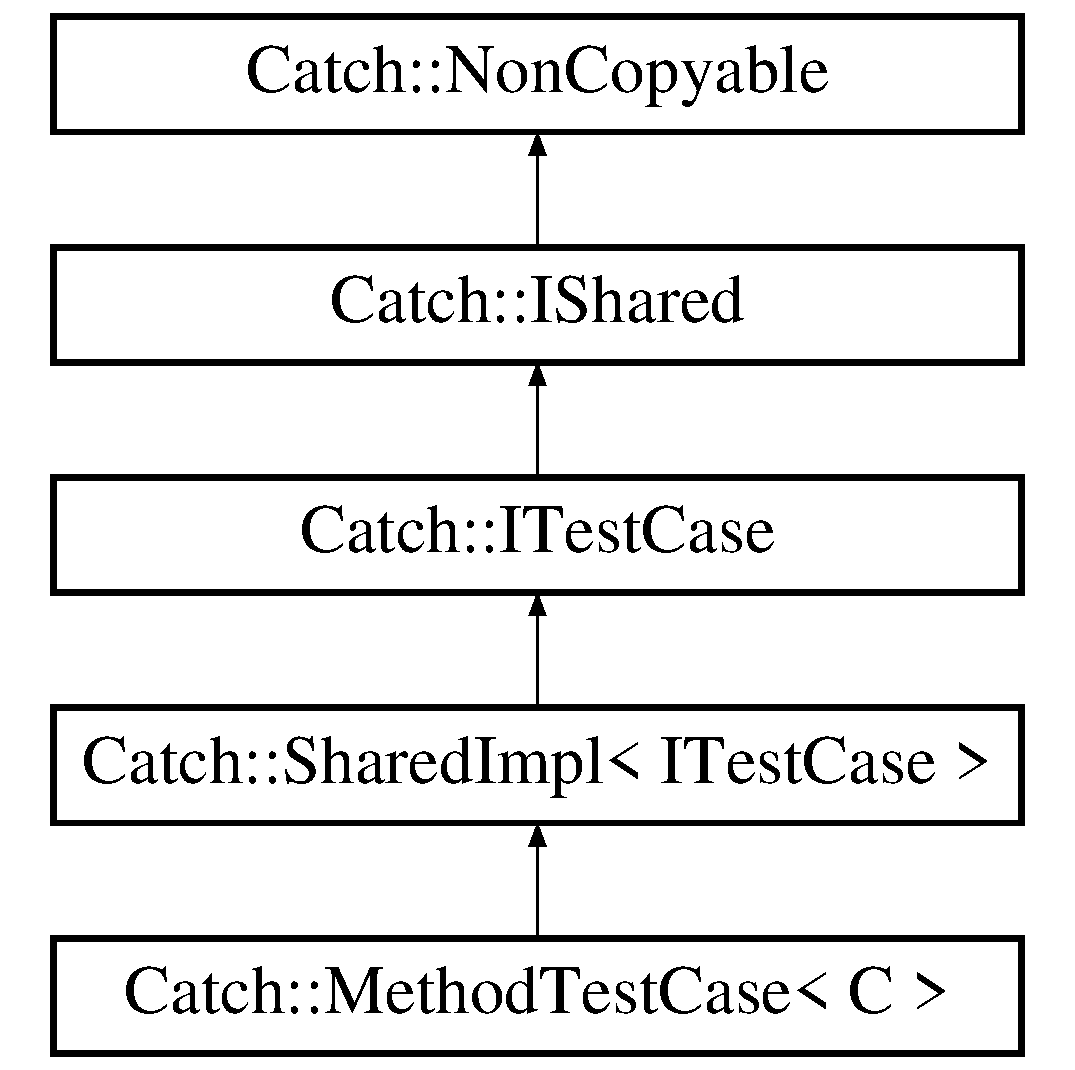
\includegraphics[height=5.000000cm]{structCatch_1_1IShared}
\end{center}
\end{figure}
\subsection*{Public Member Functions}
\begin{DoxyCompactItemize}
\item 
\mbox{\Hypertarget{structCatch_1_1IShared_ae383df68557cdaf0910b411af04d9e33}\label{structCatch_1_1IShared_ae383df68557cdaf0910b411af04d9e33}} 
virtual void {\bfseries add\+Ref} () const =0
\item 
\mbox{\Hypertarget{structCatch_1_1IShared_a002f52624728a763956fb6f230cb2f57}\label{structCatch_1_1IShared_a002f52624728a763956fb6f230cb2f57}} 
virtual void {\bfseries release} () const =0
\end{DoxyCompactItemize}


The documentation for this struct was generated from the following file\+:\begin{DoxyCompactItemize}
\item 
test\+\_\+cases/catch.\+hpp\end{DoxyCompactItemize}

\hypertarget{structCatch_1_1Detail_1_1IsStreamInsertable}{}\section{Catch\+:\+:Detail\+:\+:Is\+Stream\+Insertable$<$ T $>$ Struct Template Reference}
\label{structCatch_1_1Detail_1_1IsStreamInsertable}\index{Catch\+::\+Detail\+::\+Is\+Stream\+Insertable$<$ T $>$@{Catch\+::\+Detail\+::\+Is\+Stream\+Insertable$<$ T $>$}}
\subsection*{Public Types}
\begin{DoxyCompactItemize}
\item 
\mbox{\Hypertarget{structCatch_1_1Detail_1_1IsStreamInsertable_a2e4508694da3bf368ff67733a7970edd}\label{structCatch_1_1Detail_1_1IsStreamInsertable_a2e4508694da3bf368ff67733a7970edd}} 
enum \{ {\bfseries value} = sizeof( test\+Streamable(s $<$$<$ t) ) == sizeof( True\+Type )
 \}
\end{DoxyCompactItemize}
\subsection*{Static Public Attributes}
\begin{DoxyCompactItemize}
\item 
\mbox{\Hypertarget{structCatch_1_1Detail_1_1IsStreamInsertable_abe3d3c8e5d85665747faafffc9a96b00}\label{structCatch_1_1Detail_1_1IsStreamInsertable_abe3d3c8e5d85665747faafffc9a96b00}} 
static std\+::ostream \& {\bfseries s}
\item 
\mbox{\Hypertarget{structCatch_1_1Detail_1_1IsStreamInsertable_a7d2a3da978b6736667a7b2f6d51f507f}\label{structCatch_1_1Detail_1_1IsStreamInsertable_a7d2a3da978b6736667a7b2f6d51f507f}} 
static T const  \& {\bfseries t}
\end{DoxyCompactItemize}


The documentation for this struct was generated from the following file\+:\begin{DoxyCompactItemize}
\item 
test\+\_\+cases/catch.\+hpp\end{DoxyCompactItemize}

\hypertarget{structCatch_1_1ITagAliasRegistry}{}\section{Catch\+:\+:I\+Tag\+Alias\+Registry Struct Reference}
\label{structCatch_1_1ITagAliasRegistry}\index{Catch\+::\+I\+Tag\+Alias\+Registry@{Catch\+::\+I\+Tag\+Alias\+Registry}}
\subsection*{Public Member Functions}
\begin{DoxyCompactItemize}
\item 
\mbox{\Hypertarget{structCatch_1_1ITagAliasRegistry_a7d2fba4d39cfcc62c2695fcde4f989c3}\label{structCatch_1_1ITagAliasRegistry_a7d2fba4d39cfcc62c2695fcde4f989c3}} 
virtual \hyperlink{classCatch_1_1Option}{Option}$<$ \hyperlink{structCatch_1_1TagAlias}{Tag\+Alias} $>$ {\bfseries find} (std\+::string const \&alias) const =0
\item 
\mbox{\Hypertarget{structCatch_1_1ITagAliasRegistry_ae729a7532faf7466db1a157ce0395170}\label{structCatch_1_1ITagAliasRegistry_ae729a7532faf7466db1a157ce0395170}} 
virtual std\+::string {\bfseries expand\+Aliases} (std\+::string const \&unexpanded\+Test\+Spec) const =0
\end{DoxyCompactItemize}
\subsection*{Static Public Member Functions}
\begin{DoxyCompactItemize}
\item 
\mbox{\Hypertarget{structCatch_1_1ITagAliasRegistry_aa9d0f008f49473389c7abf6071f137a7}\label{structCatch_1_1ITagAliasRegistry_aa9d0f008f49473389c7abf6071f137a7}} 
static \hyperlink{structCatch_1_1ITagAliasRegistry}{I\+Tag\+Alias\+Registry} const  \& {\bfseries get} ()
\end{DoxyCompactItemize}


The documentation for this struct was generated from the following file\+:\begin{DoxyCompactItemize}
\item 
test\+\_\+cases/catch.\+hpp\end{DoxyCompactItemize}

\hypertarget{structCatch_1_1ITestCase}{}\section{Catch\+:\+:I\+Test\+Case Struct Reference}
\label{structCatch_1_1ITestCase}\index{Catch\+::\+I\+Test\+Case@{Catch\+::\+I\+Test\+Case}}
Inheritance diagram for Catch\+:\+:I\+Test\+Case\+:\begin{figure}[H]
\begin{center}
\leavevmode
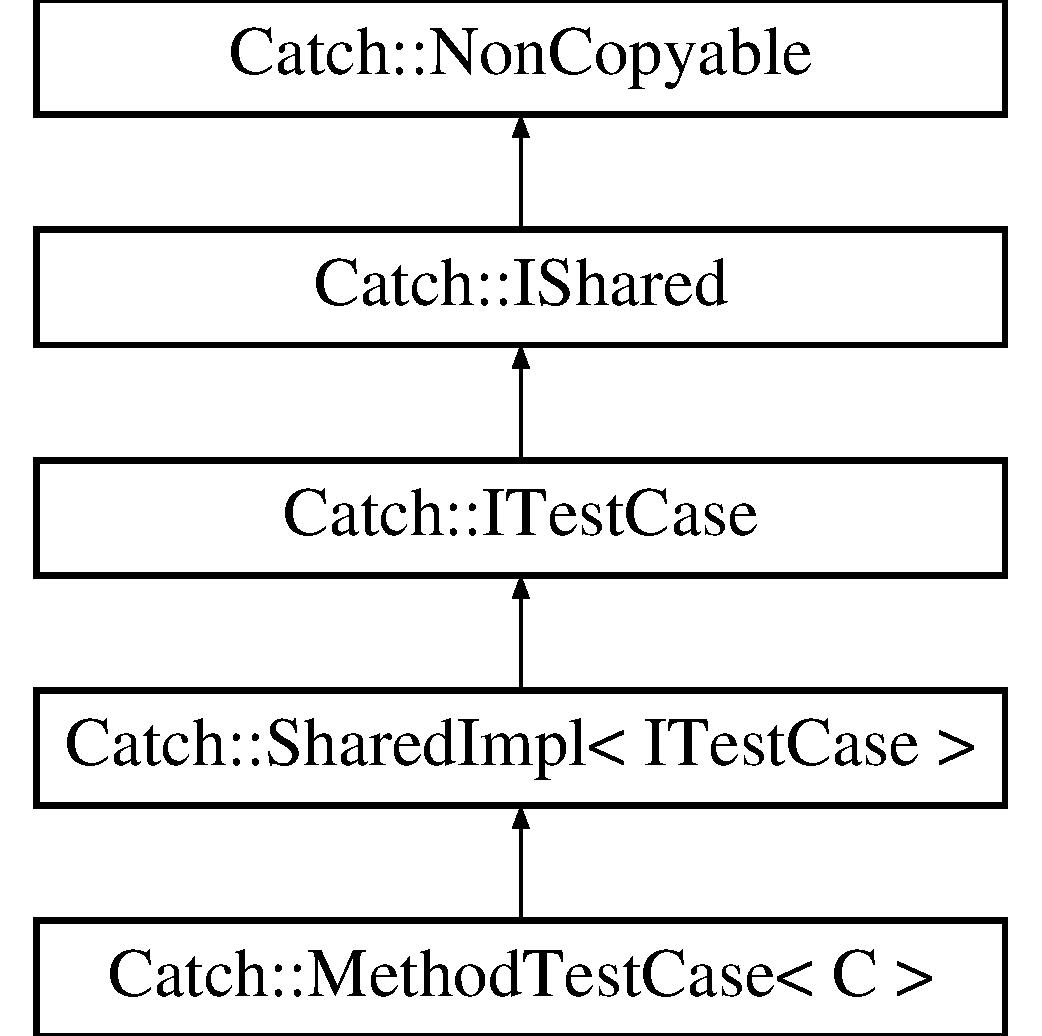
\includegraphics[height=5.000000cm]{structCatch_1_1ITestCase}
\end{center}
\end{figure}
\subsection*{Public Member Functions}
\begin{DoxyCompactItemize}
\item 
\mbox{\Hypertarget{structCatch_1_1ITestCase_a678825e62e7c17297621cfeb65588c34}\label{structCatch_1_1ITestCase_a678825e62e7c17297621cfeb65588c34}} 
virtual void {\bfseries invoke} () const =0
\end{DoxyCompactItemize}


The documentation for this struct was generated from the following file\+:\begin{DoxyCompactItemize}
\item 
test\+\_\+cases/catch.\+hpp\end{DoxyCompactItemize}

\hypertarget{structCatch_1_1ITestCaseRegistry}{}\section{Catch\+:\+:I\+Test\+Case\+Registry Struct Reference}
\label{structCatch_1_1ITestCaseRegistry}\index{Catch\+::\+I\+Test\+Case\+Registry@{Catch\+::\+I\+Test\+Case\+Registry}}
\subsection*{Public Member Functions}
\begin{DoxyCompactItemize}
\item 
\mbox{\Hypertarget{structCatch_1_1ITestCaseRegistry_ad6e4d4a621655123f73ae98cfeda063d}\label{structCatch_1_1ITestCaseRegistry_ad6e4d4a621655123f73ae98cfeda063d}} 
virtual std\+::vector$<$ \hyperlink{classCatch_1_1TestCase}{Test\+Case} $>$ const  \& {\bfseries get\+All\+Tests} () const =0
\item 
\mbox{\Hypertarget{structCatch_1_1ITestCaseRegistry_a33e46639d0319d35497c05bb5d02be5a}\label{structCatch_1_1ITestCaseRegistry_a33e46639d0319d35497c05bb5d02be5a}} 
virtual std\+::vector$<$ \hyperlink{classCatch_1_1TestCase}{Test\+Case} $>$ const  \& {\bfseries get\+All\+Tests\+Sorted} (I\+Config const \&config) const =0
\end{DoxyCompactItemize}


The documentation for this struct was generated from the following file\+:\begin{DoxyCompactItemize}
\item 
test\+\_\+cases/catch.\+hpp\end{DoxyCompactItemize}

\hypertarget{classJmpOperation}{}\section{Jmp\+Operation Class Reference}
\label{classJmpOperation}\index{Jmp\+Operation@{Jmp\+Operation}}


{\ttfamily \#include $<$Jmp\+Operation.\+h$>$}

Inheritance diagram for Jmp\+Operation\+:\begin{figure}[H]
\begin{center}
\leavevmode
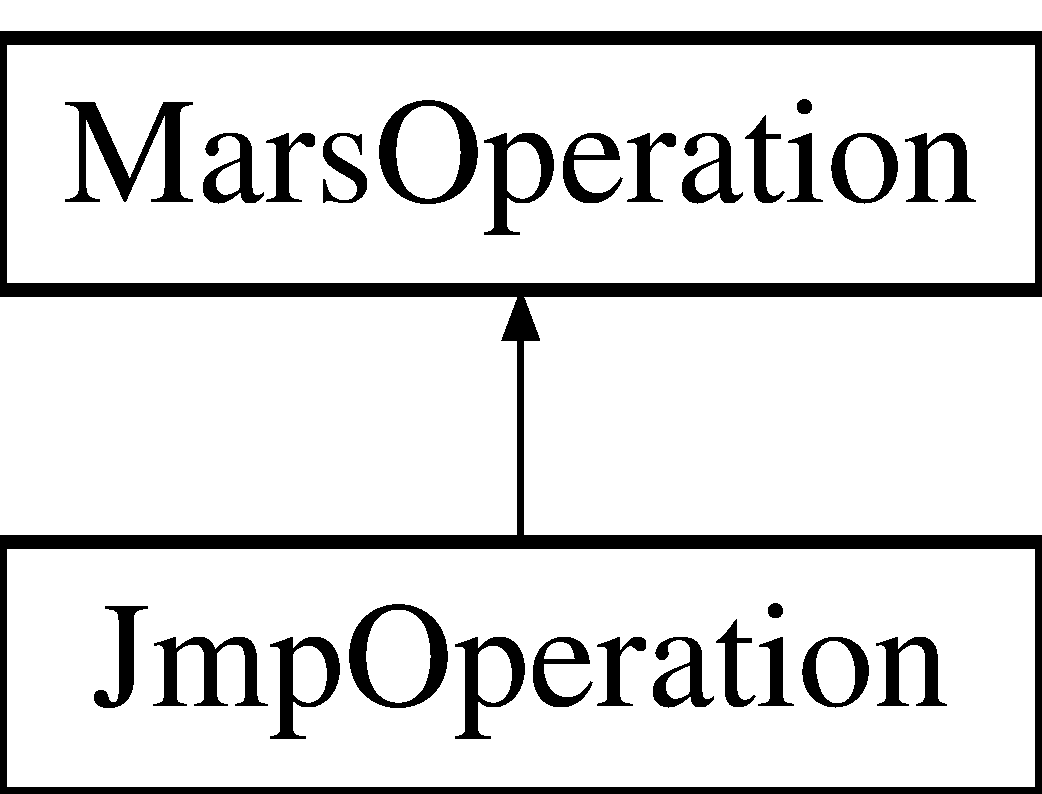
\includegraphics[height=2.000000cm]{classJmpOperation}
\end{center}
\end{figure}
\subsection*{Public Member Functions}
\begin{DoxyCompactItemize}
\item 
\mbox{\Hypertarget{classJmpOperation_a849c86f28f7fc091b7a9f46e968fd811}\label{classJmpOperation_a849c86f28f7fc091b7a9f46e968fd811}} 
virtual std\+::shared\+\_\+ptr$<$ \hyperlink{classProcessAction}{Process\+Action} $>$ {\bfseries run\+Operation} (\hyperlink{classOperationParamsInstructions}{Operation\+Params\+Instructions} $\ast$oper\+Params) override
\item 
\mbox{\Hypertarget{classJmpOperation_aeb6441bfb981138d289ee715900b2b9f}\label{classJmpOperation_aeb6441bfb981138d289ee715900b2b9f}} 
virtual std\+::shared\+\_\+ptr$<$ \hyperlink{classProcessAction}{Process\+Action} $>$ {\bfseries run\+Operation} (\hyperlink{classOperationParamsMixed}{Operation\+Params\+Mixed} $\ast$oper\+Params) override
\end{DoxyCompactItemize}


\subsection{Detailed Description}
Class representing J\+MP operation 

The documentation for this class was generated from the following files\+:\begin{DoxyCompactItemize}
\item 
logic/mars/Jmp\+Operation.\+h\item 
logic/mars/Jmp\+Operation.\+cpp\end{DoxyCompactItemize}

\hypertarget{classMainController}{}\section{Main\+Controller Class Reference}
\label{classMainController}\index{Main\+Controller@{Main\+Controller}}
\subsection*{Public Member Functions}
\begin{DoxyCompactItemize}
\item 
void \hyperlink{classMainController_a2dc81550fb4ac999e6c1827518fa0830}{run} ()
\end{DoxyCompactItemize}


\subsection{Member Function Documentation}
\mbox{\Hypertarget{classMainController_a2dc81550fb4ac999e6c1827518fa0830}\label{classMainController_a2dc81550fb4ac999e6c1827518fa0830}} 
\index{Main\+Controller@{Main\+Controller}!run@{run}}
\index{run@{run}!Main\+Controller@{Main\+Controller}}
\subsubsection{\texorpdfstring{run()}{run()}}
{\footnotesize\ttfamily void Main\+Controller\+::run (\begin{DoxyParamCaption}{ }\end{DoxyParamCaption})}

Main loop of c++ client 

The documentation for this class was generated from the following files\+:\begin{DoxyCompactItemize}
\item 
logic/Main\+Controller.\+h\item 
logic/Main\+Controller.\+cpp\end{DoxyCompactItemize}

\hypertarget{classMARS_1_1MARS__getCode__args}{}\section{M\+A\+RS\+:\+:M\+A\+R\+S\+\_\+get\+Code\+\_\+args Class Reference}
\label{classMARS_1_1MARS__getCode__args}\index{M\+A\+R\+S\+::\+M\+A\+R\+S\+\_\+get\+Code\+\_\+args@{M\+A\+R\+S\+::\+M\+A\+R\+S\+\_\+get\+Code\+\_\+args}}
\subsection*{Public Member Functions}
\begin{DoxyCompactItemize}
\item 
\mbox{\Hypertarget{classMARS_1_1MARS__getCode__args_a98c32ba2c7415512e87088bfb02838e3}\label{classMARS_1_1MARS__getCode__args_a98c32ba2c7415512e87088bfb02838e3}} 
{\bfseries M\+A\+R\+S\+\_\+get\+Code\+\_\+args} (const \hyperlink{classMARS_1_1MARS__getCode__args}{M\+A\+R\+S\+\_\+get\+Code\+\_\+args} \&)
\item 
\mbox{\Hypertarget{classMARS_1_1MARS__getCode__args_abf1b0524b84708a105a766ea6fdee220}\label{classMARS_1_1MARS__getCode__args_abf1b0524b84708a105a766ea6fdee220}} 
\hyperlink{classMARS_1_1MARS__getCode__args}{M\+A\+R\+S\+\_\+get\+Code\+\_\+args} \& {\bfseries operator=} (const \hyperlink{classMARS_1_1MARS__getCode__args}{M\+A\+R\+S\+\_\+get\+Code\+\_\+args} \&)
\item 
\mbox{\Hypertarget{classMARS_1_1MARS__getCode__args_a538f5b261df08d963a02673b40d2cd2e}\label{classMARS_1_1MARS__getCode__args_a538f5b261df08d963a02673b40d2cd2e}} 
bool {\bfseries operator==} (const \hyperlink{classMARS_1_1MARS__getCode__args}{M\+A\+R\+S\+\_\+get\+Code\+\_\+args} \&) const
\item 
\mbox{\Hypertarget{classMARS_1_1MARS__getCode__args_a2ea346271af181ad82ea513ec33223a1}\label{classMARS_1_1MARS__getCode__args_a2ea346271af181ad82ea513ec33223a1}} 
bool {\bfseries operator!=} (const \hyperlink{classMARS_1_1MARS__getCode__args}{M\+A\+R\+S\+\_\+get\+Code\+\_\+args} \&rhs) const
\item 
\mbox{\Hypertarget{classMARS_1_1MARS__getCode__args_a30b1d9ebc0de427fc01f9c43e2932a4c}\label{classMARS_1_1MARS__getCode__args_a30b1d9ebc0de427fc01f9c43e2932a4c}} 
bool {\bfseries operator$<$} (const \hyperlink{classMARS_1_1MARS__getCode__args}{M\+A\+R\+S\+\_\+get\+Code\+\_\+args} \&) const
\item 
\mbox{\Hypertarget{classMARS_1_1MARS__getCode__args_a9b6e0b5c816f90646a11e33d0bd1aee2}\label{classMARS_1_1MARS__getCode__args_a9b6e0b5c816f90646a11e33d0bd1aee2}} 
uint32\+\_\+t {\bfseries read} (\+::apache\+::thrift\+::protocol\+::\+T\+Protocol $\ast$iprot)
\item 
\mbox{\Hypertarget{classMARS_1_1MARS__getCode__args_a8f08cc0c9f18499b551200d9674e9ac2}\label{classMARS_1_1MARS__getCode__args_a8f08cc0c9f18499b551200d9674e9ac2}} 
uint32\+\_\+t {\bfseries write} (\+::apache\+::thrift\+::protocol\+::\+T\+Protocol $\ast$oprot) const
\end{DoxyCompactItemize}


The documentation for this class was generated from the following files\+:\begin{DoxyCompactItemize}
\item 
gen-\/cpp/M\+A\+R\+S.\+h\item 
gen-\/cpp/M\+A\+R\+S.\+cpp\end{DoxyCompactItemize}

\hypertarget{classMARS_1_1MARS__getCode__pargs}{}\section{M\+A\+RS\+:\+:M\+A\+R\+S\+\_\+get\+Code\+\_\+pargs Class Reference}
\label{classMARS_1_1MARS__getCode__pargs}\index{M\+A\+R\+S\+::\+M\+A\+R\+S\+\_\+get\+Code\+\_\+pargs@{M\+A\+R\+S\+::\+M\+A\+R\+S\+\_\+get\+Code\+\_\+pargs}}
\subsection*{Public Member Functions}
\begin{DoxyCompactItemize}
\item 
\mbox{\Hypertarget{classMARS_1_1MARS__getCode__pargs_a2cba857b0354dbc6a8f1f56e5798e3f7}\label{classMARS_1_1MARS__getCode__pargs_a2cba857b0354dbc6a8f1f56e5798e3f7}} 
uint32\+\_\+t {\bfseries write} (\+::apache\+::thrift\+::protocol\+::\+T\+Protocol $\ast$oprot) const
\end{DoxyCompactItemize}


The documentation for this class was generated from the following files\+:\begin{DoxyCompactItemize}
\item 
gen-\/cpp/M\+A\+R\+S.\+h\item 
gen-\/cpp/M\+A\+R\+S.\+cpp\end{DoxyCompactItemize}

\hypertarget{classMARS_1_1MARS__getCode__presult}{}\section{M\+A\+RS\+:\+:M\+A\+R\+S\+\_\+get\+Code\+\_\+presult Class Reference}
\label{classMARS_1_1MARS__getCode__presult}\index{M\+A\+R\+S\+::\+M\+A\+R\+S\+\_\+get\+Code\+\_\+presult@{M\+A\+R\+S\+::\+M\+A\+R\+S\+\_\+get\+Code\+\_\+presult}}
\subsection*{Public Member Functions}
\begin{DoxyCompactItemize}
\item 
\mbox{\Hypertarget{classMARS_1_1MARS__getCode__presult_a6f4847fe64084025d7f8ed311281a800}\label{classMARS_1_1MARS__getCode__presult_a6f4847fe64084025d7f8ed311281a800}} 
uint32\+\_\+t {\bfseries read} (\+::apache\+::thrift\+::protocol\+::\+T\+Protocol $\ast$iprot)
\end{DoxyCompactItemize}
\subsection*{Public Attributes}
\begin{DoxyCompactItemize}
\item 
\mbox{\Hypertarget{classMARS_1_1MARS__getCode__presult_a22629788323ebe3c8f7c0cf710657ad6}\label{classMARS_1_1MARS__getCode__presult_a22629788323ebe3c8f7c0cf710657ad6}} 
std\+::string $\ast$ {\bfseries success}
\item 
\mbox{\Hypertarget{classMARS_1_1MARS__getCode__presult_ad0ab0a2e93de6852ab4c5b160c93c778}\label{classMARS_1_1MARS__getCode__presult_ad0ab0a2e93de6852ab4c5b160c93c778}} 
\hyperlink{structMARS_1_1__MARS__getCode__presult____isset}{\+\_\+\+M\+A\+R\+S\+\_\+get\+Code\+\_\+presult\+\_\+\+\_\+isset} {\bfseries \+\_\+\+\_\+isset}
\end{DoxyCompactItemize}


The documentation for this class was generated from the following files\+:\begin{DoxyCompactItemize}
\item 
gen-\/cpp/M\+A\+R\+S.\+h\item 
gen-\/cpp/M\+A\+R\+S.\+cpp\end{DoxyCompactItemize}

\hypertarget{classMARS_1_1MARS__getCode__result}{}\section{M\+A\+RS\+:\+:M\+A\+R\+S\+\_\+get\+Code\+\_\+result Class Reference}
\label{classMARS_1_1MARS__getCode__result}\index{M\+A\+R\+S\+::\+M\+A\+R\+S\+\_\+get\+Code\+\_\+result@{M\+A\+R\+S\+::\+M\+A\+R\+S\+\_\+get\+Code\+\_\+result}}
\subsection*{Public Member Functions}
\begin{DoxyCompactItemize}
\item 
\mbox{\Hypertarget{classMARS_1_1MARS__getCode__result_a20d2bdf4d545dfe57c1b083650bfedb4}\label{classMARS_1_1MARS__getCode__result_a20d2bdf4d545dfe57c1b083650bfedb4}} 
{\bfseries M\+A\+R\+S\+\_\+get\+Code\+\_\+result} (const \hyperlink{classMARS_1_1MARS__getCode__result}{M\+A\+R\+S\+\_\+get\+Code\+\_\+result} \&)
\item 
\mbox{\Hypertarget{classMARS_1_1MARS__getCode__result_a0dda8f4061fc5f85e20324d707ead5b3}\label{classMARS_1_1MARS__getCode__result_a0dda8f4061fc5f85e20324d707ead5b3}} 
\hyperlink{classMARS_1_1MARS__getCode__result}{M\+A\+R\+S\+\_\+get\+Code\+\_\+result} \& {\bfseries operator=} (const \hyperlink{classMARS_1_1MARS__getCode__result}{M\+A\+R\+S\+\_\+get\+Code\+\_\+result} \&)
\item 
\mbox{\Hypertarget{classMARS_1_1MARS__getCode__result_a55feb1697ab48cc57a11eb766104e8fb}\label{classMARS_1_1MARS__getCode__result_a55feb1697ab48cc57a11eb766104e8fb}} 
void {\bfseries \+\_\+\+\_\+set\+\_\+success} (const std\+::string \&val)
\item 
\mbox{\Hypertarget{classMARS_1_1MARS__getCode__result_a52cef84f125e7a7f9396cd1805da3803}\label{classMARS_1_1MARS__getCode__result_a52cef84f125e7a7f9396cd1805da3803}} 
bool {\bfseries operator==} (const \hyperlink{classMARS_1_1MARS__getCode__result}{M\+A\+R\+S\+\_\+get\+Code\+\_\+result} \&rhs) const
\item 
\mbox{\Hypertarget{classMARS_1_1MARS__getCode__result_ad3790389d7d8f9e14598206efe69aa26}\label{classMARS_1_1MARS__getCode__result_ad3790389d7d8f9e14598206efe69aa26}} 
bool {\bfseries operator!=} (const \hyperlink{classMARS_1_1MARS__getCode__result}{M\+A\+R\+S\+\_\+get\+Code\+\_\+result} \&rhs) const
\item 
\mbox{\Hypertarget{classMARS_1_1MARS__getCode__result_aeaa576da7821a43065eca7324565532b}\label{classMARS_1_1MARS__getCode__result_aeaa576da7821a43065eca7324565532b}} 
bool {\bfseries operator$<$} (const \hyperlink{classMARS_1_1MARS__getCode__result}{M\+A\+R\+S\+\_\+get\+Code\+\_\+result} \&) const
\item 
\mbox{\Hypertarget{classMARS_1_1MARS__getCode__result_a42818fa2e6f345f111601ca7b4399b86}\label{classMARS_1_1MARS__getCode__result_a42818fa2e6f345f111601ca7b4399b86}} 
uint32\+\_\+t {\bfseries read} (\+::apache\+::thrift\+::protocol\+::\+T\+Protocol $\ast$iprot)
\item 
\mbox{\Hypertarget{classMARS_1_1MARS__getCode__result_acf9b9722bedd470e38cffb2bf22d2eb6}\label{classMARS_1_1MARS__getCode__result_acf9b9722bedd470e38cffb2bf22d2eb6}} 
uint32\+\_\+t {\bfseries write} (\+::apache\+::thrift\+::protocol\+::\+T\+Protocol $\ast$oprot) const
\end{DoxyCompactItemize}
\subsection*{Public Attributes}
\begin{DoxyCompactItemize}
\item 
\mbox{\Hypertarget{classMARS_1_1MARS__getCode__result_a4f0666ceac16cdb8b86841f5a20519ce}\label{classMARS_1_1MARS__getCode__result_a4f0666ceac16cdb8b86841f5a20519ce}} 
std\+::string {\bfseries success}
\item 
\mbox{\Hypertarget{classMARS_1_1MARS__getCode__result_a58d63f9c0a57c3143820120ec6219e89}\label{classMARS_1_1MARS__getCode__result_a58d63f9c0a57c3143820120ec6219e89}} 
\hyperlink{structMARS_1_1__MARS__getCode__result____isset}{\+\_\+\+M\+A\+R\+S\+\_\+get\+Code\+\_\+result\+\_\+\+\_\+isset} {\bfseries \+\_\+\+\_\+isset}
\end{DoxyCompactItemize}


The documentation for this class was generated from the following files\+:\begin{DoxyCompactItemize}
\item 
gen-\/cpp/M\+A\+R\+S.\+h\item 
gen-\/cpp/M\+A\+R\+S.\+cpp\end{DoxyCompactItemize}

\hypertarget{classMARS_1_1MARS__getColorTable__args}{}\section{M\+A\+RS\+:\+:M\+A\+R\+S\+\_\+get\+Color\+Table\+\_\+args Class Reference}
\label{classMARS_1_1MARS__getColorTable__args}\index{M\+A\+R\+S\+::\+M\+A\+R\+S\+\_\+get\+Color\+Table\+\_\+args@{M\+A\+R\+S\+::\+M\+A\+R\+S\+\_\+get\+Color\+Table\+\_\+args}}
\subsection*{Public Member Functions}
\begin{DoxyCompactItemize}
\item 
\mbox{\Hypertarget{classMARS_1_1MARS__getColorTable__args_a8281babd6a3c80608b489c69badb4474}\label{classMARS_1_1MARS__getColorTable__args_a8281babd6a3c80608b489c69badb4474}} 
{\bfseries M\+A\+R\+S\+\_\+get\+Color\+Table\+\_\+args} (const \hyperlink{classMARS_1_1MARS__getColorTable__args}{M\+A\+R\+S\+\_\+get\+Color\+Table\+\_\+args} \&)
\item 
\mbox{\Hypertarget{classMARS_1_1MARS__getColorTable__args_a741536fc92f8da49ac383cdb98035117}\label{classMARS_1_1MARS__getColorTable__args_a741536fc92f8da49ac383cdb98035117}} 
\hyperlink{classMARS_1_1MARS__getColorTable__args}{M\+A\+R\+S\+\_\+get\+Color\+Table\+\_\+args} \& {\bfseries operator=} (const \hyperlink{classMARS_1_1MARS__getColorTable__args}{M\+A\+R\+S\+\_\+get\+Color\+Table\+\_\+args} \&)
\item 
\mbox{\Hypertarget{classMARS_1_1MARS__getColorTable__args_a1a6ebf22a52b65ee6e5e6261795b2153}\label{classMARS_1_1MARS__getColorTable__args_a1a6ebf22a52b65ee6e5e6261795b2153}} 
bool {\bfseries operator==} (const \hyperlink{classMARS_1_1MARS__getColorTable__args}{M\+A\+R\+S\+\_\+get\+Color\+Table\+\_\+args} \&) const
\item 
\mbox{\Hypertarget{classMARS_1_1MARS__getColorTable__args_a4a0f545f35ea6bca03c384f2692b11d2}\label{classMARS_1_1MARS__getColorTable__args_a4a0f545f35ea6bca03c384f2692b11d2}} 
bool {\bfseries operator!=} (const \hyperlink{classMARS_1_1MARS__getColorTable__args}{M\+A\+R\+S\+\_\+get\+Color\+Table\+\_\+args} \&rhs) const
\item 
\mbox{\Hypertarget{classMARS_1_1MARS__getColorTable__args_ada928ce883b979eb7bca7a50bff59eaa}\label{classMARS_1_1MARS__getColorTable__args_ada928ce883b979eb7bca7a50bff59eaa}} 
bool {\bfseries operator$<$} (const \hyperlink{classMARS_1_1MARS__getColorTable__args}{M\+A\+R\+S\+\_\+get\+Color\+Table\+\_\+args} \&) const
\item 
\mbox{\Hypertarget{classMARS_1_1MARS__getColorTable__args_a8cd721f30388cdb5358f2f41e3b4ea15}\label{classMARS_1_1MARS__getColorTable__args_a8cd721f30388cdb5358f2f41e3b4ea15}} 
uint32\+\_\+t {\bfseries read} (\+::apache\+::thrift\+::protocol\+::\+T\+Protocol $\ast$iprot)
\item 
\mbox{\Hypertarget{classMARS_1_1MARS__getColorTable__args_a03174ef7e3f9b34d2b676a96711b6709}\label{classMARS_1_1MARS__getColorTable__args_a03174ef7e3f9b34d2b676a96711b6709}} 
uint32\+\_\+t {\bfseries write} (\+::apache\+::thrift\+::protocol\+::\+T\+Protocol $\ast$oprot) const
\end{DoxyCompactItemize}


The documentation for this class was generated from the following files\+:\begin{DoxyCompactItemize}
\item 
gen-\/cpp/M\+A\+R\+S.\+h\item 
gen-\/cpp/M\+A\+R\+S.\+cpp\end{DoxyCompactItemize}

\hypertarget{classMARS_1_1MARS__getColorTable__pargs}{}\section{M\+A\+RS\+:\+:M\+A\+R\+S\+\_\+get\+Color\+Table\+\_\+pargs Class Reference}
\label{classMARS_1_1MARS__getColorTable__pargs}\index{M\+A\+R\+S\+::\+M\+A\+R\+S\+\_\+get\+Color\+Table\+\_\+pargs@{M\+A\+R\+S\+::\+M\+A\+R\+S\+\_\+get\+Color\+Table\+\_\+pargs}}
\subsection*{Public Member Functions}
\begin{DoxyCompactItemize}
\item 
\mbox{\Hypertarget{classMARS_1_1MARS__getColorTable__pargs_a91f473e60c3af3f843d1de77bab011cc}\label{classMARS_1_1MARS__getColorTable__pargs_a91f473e60c3af3f843d1de77bab011cc}} 
uint32\+\_\+t {\bfseries write} (\+::apache\+::thrift\+::protocol\+::\+T\+Protocol $\ast$oprot) const
\end{DoxyCompactItemize}


The documentation for this class was generated from the following files\+:\begin{DoxyCompactItemize}
\item 
gen-\/cpp/M\+A\+R\+S.\+h\item 
gen-\/cpp/M\+A\+R\+S.\+cpp\end{DoxyCompactItemize}

\hypertarget{classMARS_1_1MARS__getColorTable__presult}{}\section{M\+A\+RS\+:\+:M\+A\+R\+S\+\_\+get\+Color\+Table\+\_\+presult Class Reference}
\label{classMARS_1_1MARS__getColorTable__presult}\index{M\+A\+R\+S\+::\+M\+A\+R\+S\+\_\+get\+Color\+Table\+\_\+presult@{M\+A\+R\+S\+::\+M\+A\+R\+S\+\_\+get\+Color\+Table\+\_\+presult}}
\subsection*{Public Member Functions}
\begin{DoxyCompactItemize}
\item 
\mbox{\Hypertarget{classMARS_1_1MARS__getColorTable__presult_a4fd9ef8e10f9916b78c2d9639942c298}\label{classMARS_1_1MARS__getColorTable__presult_a4fd9ef8e10f9916b78c2d9639942c298}} 
uint32\+\_\+t {\bfseries read} (\+::apache\+::thrift\+::protocol\+::\+T\+Protocol $\ast$iprot)
\end{DoxyCompactItemize}
\subsection*{Public Attributes}
\begin{DoxyCompactItemize}
\item 
\mbox{\Hypertarget{classMARS_1_1MARS__getColorTable__presult_adbbe7ee81a4ddcb9fe4b58f1b9355d9f}\label{classMARS_1_1MARS__getColorTable__presult_adbbe7ee81a4ddcb9fe4b58f1b9355d9f}} 
std\+::vector$<$ std\+::string $>$ $\ast$ {\bfseries success}
\item 
\mbox{\Hypertarget{classMARS_1_1MARS__getColorTable__presult_a9ffc65771ae7ce3f4c2af348b85cf534}\label{classMARS_1_1MARS__getColorTable__presult_a9ffc65771ae7ce3f4c2af348b85cf534}} 
\hyperlink{structMARS_1_1__MARS__getColorTable__presult____isset}{\+\_\+\+M\+A\+R\+S\+\_\+get\+Color\+Table\+\_\+presult\+\_\+\+\_\+isset} {\bfseries \+\_\+\+\_\+isset}
\end{DoxyCompactItemize}


The documentation for this class was generated from the following files\+:\begin{DoxyCompactItemize}
\item 
gen-\/cpp/M\+A\+R\+S.\+h\item 
gen-\/cpp/M\+A\+R\+S.\+cpp\end{DoxyCompactItemize}

\hypertarget{classMARS_1_1MARS__getColorTable__result}{}\section{M\+A\+RS\+:\+:M\+A\+R\+S\+\_\+get\+Color\+Table\+\_\+result Class Reference}
\label{classMARS_1_1MARS__getColorTable__result}\index{M\+A\+R\+S\+::\+M\+A\+R\+S\+\_\+get\+Color\+Table\+\_\+result@{M\+A\+R\+S\+::\+M\+A\+R\+S\+\_\+get\+Color\+Table\+\_\+result}}
\subsection*{Public Member Functions}
\begin{DoxyCompactItemize}
\item 
\mbox{\Hypertarget{classMARS_1_1MARS__getColorTable__result_a42f9c853c5fe23fd1f3c6c6f3c87d2fa}\label{classMARS_1_1MARS__getColorTable__result_a42f9c853c5fe23fd1f3c6c6f3c87d2fa}} 
{\bfseries M\+A\+R\+S\+\_\+get\+Color\+Table\+\_\+result} (const \hyperlink{classMARS_1_1MARS__getColorTable__result}{M\+A\+R\+S\+\_\+get\+Color\+Table\+\_\+result} \&)
\item 
\mbox{\Hypertarget{classMARS_1_1MARS__getColorTable__result_a3c4c5e148ae5bfb819e7a2a93eb5a233}\label{classMARS_1_1MARS__getColorTable__result_a3c4c5e148ae5bfb819e7a2a93eb5a233}} 
\hyperlink{classMARS_1_1MARS__getColorTable__result}{M\+A\+R\+S\+\_\+get\+Color\+Table\+\_\+result} \& {\bfseries operator=} (const \hyperlink{classMARS_1_1MARS__getColorTable__result}{M\+A\+R\+S\+\_\+get\+Color\+Table\+\_\+result} \&)
\item 
\mbox{\Hypertarget{classMARS_1_1MARS__getColorTable__result_a8796b7db20a0b2d8bcc761fb66c3b52e}\label{classMARS_1_1MARS__getColorTable__result_a8796b7db20a0b2d8bcc761fb66c3b52e}} 
void {\bfseries \+\_\+\+\_\+set\+\_\+success} (const std\+::vector$<$ std\+::string $>$ \&val)
\item 
\mbox{\Hypertarget{classMARS_1_1MARS__getColorTable__result_a94a26d274dc54acbe961a0863d0d7f63}\label{classMARS_1_1MARS__getColorTable__result_a94a26d274dc54acbe961a0863d0d7f63}} 
bool {\bfseries operator==} (const \hyperlink{classMARS_1_1MARS__getColorTable__result}{M\+A\+R\+S\+\_\+get\+Color\+Table\+\_\+result} \&rhs) const
\item 
\mbox{\Hypertarget{classMARS_1_1MARS__getColorTable__result_a8cd8918418289948cea247563b36a5aa}\label{classMARS_1_1MARS__getColorTable__result_a8cd8918418289948cea247563b36a5aa}} 
bool {\bfseries operator!=} (const \hyperlink{classMARS_1_1MARS__getColorTable__result}{M\+A\+R\+S\+\_\+get\+Color\+Table\+\_\+result} \&rhs) const
\item 
\mbox{\Hypertarget{classMARS_1_1MARS__getColorTable__result_adcc9196065c8028b7cb792698a44735b}\label{classMARS_1_1MARS__getColorTable__result_adcc9196065c8028b7cb792698a44735b}} 
bool {\bfseries operator$<$} (const \hyperlink{classMARS_1_1MARS__getColorTable__result}{M\+A\+R\+S\+\_\+get\+Color\+Table\+\_\+result} \&) const
\item 
\mbox{\Hypertarget{classMARS_1_1MARS__getColorTable__result_a6a6d7f7aabc39052bbbe00b75a06fe3b}\label{classMARS_1_1MARS__getColorTable__result_a6a6d7f7aabc39052bbbe00b75a06fe3b}} 
uint32\+\_\+t {\bfseries read} (\+::apache\+::thrift\+::protocol\+::\+T\+Protocol $\ast$iprot)
\item 
\mbox{\Hypertarget{classMARS_1_1MARS__getColorTable__result_ae897d516d900713921c510d23a4a4dee}\label{classMARS_1_1MARS__getColorTable__result_ae897d516d900713921c510d23a4a4dee}} 
uint32\+\_\+t {\bfseries write} (\+::apache\+::thrift\+::protocol\+::\+T\+Protocol $\ast$oprot) const
\end{DoxyCompactItemize}
\subsection*{Public Attributes}
\begin{DoxyCompactItemize}
\item 
\mbox{\Hypertarget{classMARS_1_1MARS__getColorTable__result_ad451b498aecd8356d94853586cdb1bf8}\label{classMARS_1_1MARS__getColorTable__result_ad451b498aecd8356d94853586cdb1bf8}} 
std\+::vector$<$ std\+::string $>$ {\bfseries success}
\item 
\mbox{\Hypertarget{classMARS_1_1MARS__getColorTable__result_a5969aa2f5c72ddaf03bba6bc2359905d}\label{classMARS_1_1MARS__getColorTable__result_a5969aa2f5c72ddaf03bba6bc2359905d}} 
\hyperlink{structMARS_1_1__MARS__getColorTable__result____isset}{\+\_\+\+M\+A\+R\+S\+\_\+get\+Color\+Table\+\_\+result\+\_\+\+\_\+isset} {\bfseries \+\_\+\+\_\+isset}
\end{DoxyCompactItemize}


The documentation for this class was generated from the following files\+:\begin{DoxyCompactItemize}
\item 
gen-\/cpp/M\+A\+R\+S.\+h\item 
gen-\/cpp/M\+A\+R\+S.\+cpp\end{DoxyCompactItemize}

\hypertarget{classMARS_1_1MARS__getMessage__args}{}\section{M\+A\+RS\+:\+:M\+A\+R\+S\+\_\+get\+Message\+\_\+args Class Reference}
\label{classMARS_1_1MARS__getMessage__args}\index{M\+A\+R\+S\+::\+M\+A\+R\+S\+\_\+get\+Message\+\_\+args@{M\+A\+R\+S\+::\+M\+A\+R\+S\+\_\+get\+Message\+\_\+args}}
\subsection*{Public Member Functions}
\begin{DoxyCompactItemize}
\item 
\mbox{\Hypertarget{classMARS_1_1MARS__getMessage__args_a4356f7af49401852ba8444ec96155bcd}\label{classMARS_1_1MARS__getMessage__args_a4356f7af49401852ba8444ec96155bcd}} 
{\bfseries M\+A\+R\+S\+\_\+get\+Message\+\_\+args} (const \hyperlink{classMARS_1_1MARS__getMessage__args}{M\+A\+R\+S\+\_\+get\+Message\+\_\+args} \&)
\item 
\mbox{\Hypertarget{classMARS_1_1MARS__getMessage__args_ab20c3fee80dd01c8532859344be116f8}\label{classMARS_1_1MARS__getMessage__args_ab20c3fee80dd01c8532859344be116f8}} 
\hyperlink{classMARS_1_1MARS__getMessage__args}{M\+A\+R\+S\+\_\+get\+Message\+\_\+args} \& {\bfseries operator=} (const \hyperlink{classMARS_1_1MARS__getMessage__args}{M\+A\+R\+S\+\_\+get\+Message\+\_\+args} \&)
\item 
\mbox{\Hypertarget{classMARS_1_1MARS__getMessage__args_a020731a2c36ff976198c9d63db6094f8}\label{classMARS_1_1MARS__getMessage__args_a020731a2c36ff976198c9d63db6094f8}} 
void {\bfseries \+\_\+\+\_\+set\+\_\+message} (const std\+::string \&val)
\item 
\mbox{\Hypertarget{classMARS_1_1MARS__getMessage__args_a9d556a6becac3ce1d146d3dd7b576a9d}\label{classMARS_1_1MARS__getMessage__args_a9d556a6becac3ce1d146d3dd7b576a9d}} 
bool {\bfseries operator==} (const \hyperlink{classMARS_1_1MARS__getMessage__args}{M\+A\+R\+S\+\_\+get\+Message\+\_\+args} \&rhs) const
\item 
\mbox{\Hypertarget{classMARS_1_1MARS__getMessage__args_aad5327644123e73e9588912301db109c}\label{classMARS_1_1MARS__getMessage__args_aad5327644123e73e9588912301db109c}} 
bool {\bfseries operator!=} (const \hyperlink{classMARS_1_1MARS__getMessage__args}{M\+A\+R\+S\+\_\+get\+Message\+\_\+args} \&rhs) const
\item 
\mbox{\Hypertarget{classMARS_1_1MARS__getMessage__args_afe412a8ea0b5d5739ef707e9dffdcd41}\label{classMARS_1_1MARS__getMessage__args_afe412a8ea0b5d5739ef707e9dffdcd41}} 
bool {\bfseries operator$<$} (const \hyperlink{classMARS_1_1MARS__getMessage__args}{M\+A\+R\+S\+\_\+get\+Message\+\_\+args} \&) const
\item 
\mbox{\Hypertarget{classMARS_1_1MARS__getMessage__args_af65cb8e7c539f59589aa0034727ed7f2}\label{classMARS_1_1MARS__getMessage__args_af65cb8e7c539f59589aa0034727ed7f2}} 
uint32\+\_\+t {\bfseries read} (\+::apache\+::thrift\+::protocol\+::\+T\+Protocol $\ast$iprot)
\item 
\mbox{\Hypertarget{classMARS_1_1MARS__getMessage__args_a30962f2a62afa2b64b644654a964cb69}\label{classMARS_1_1MARS__getMessage__args_a30962f2a62afa2b64b644654a964cb69}} 
uint32\+\_\+t {\bfseries write} (\+::apache\+::thrift\+::protocol\+::\+T\+Protocol $\ast$oprot) const
\end{DoxyCompactItemize}
\subsection*{Public Attributes}
\begin{DoxyCompactItemize}
\item 
\mbox{\Hypertarget{classMARS_1_1MARS__getMessage__args_a7dc8c0eaddecd6c6b9622c1af318df37}\label{classMARS_1_1MARS__getMessage__args_a7dc8c0eaddecd6c6b9622c1af318df37}} 
std\+::string {\bfseries message}
\item 
\mbox{\Hypertarget{classMARS_1_1MARS__getMessage__args_a8350ca66491bbe826b385c8af38701db}\label{classMARS_1_1MARS__getMessage__args_a8350ca66491bbe826b385c8af38701db}} 
\hyperlink{structMARS_1_1__MARS__getMessage__args____isset}{\+\_\+\+M\+A\+R\+S\+\_\+get\+Message\+\_\+args\+\_\+\+\_\+isset} {\bfseries \+\_\+\+\_\+isset}
\end{DoxyCompactItemize}


The documentation for this class was generated from the following files\+:\begin{DoxyCompactItemize}
\item 
gen-\/cpp/M\+A\+R\+S.\+h\item 
gen-\/cpp/M\+A\+R\+S.\+cpp\end{DoxyCompactItemize}

\hypertarget{classMARS_1_1MARS__getMessage__pargs}{}\section{M\+A\+RS\+:\+:M\+A\+R\+S\+\_\+get\+Message\+\_\+pargs Class Reference}
\label{classMARS_1_1MARS__getMessage__pargs}\index{M\+A\+R\+S\+::\+M\+A\+R\+S\+\_\+get\+Message\+\_\+pargs@{M\+A\+R\+S\+::\+M\+A\+R\+S\+\_\+get\+Message\+\_\+pargs}}
\subsection*{Public Member Functions}
\begin{DoxyCompactItemize}
\item 
\mbox{\Hypertarget{classMARS_1_1MARS__getMessage__pargs_a50c8af87683ea01e4b83acbae21e3abc}\label{classMARS_1_1MARS__getMessage__pargs_a50c8af87683ea01e4b83acbae21e3abc}} 
uint32\+\_\+t {\bfseries write} (\+::apache\+::thrift\+::protocol\+::\+T\+Protocol $\ast$oprot) const
\end{DoxyCompactItemize}
\subsection*{Public Attributes}
\begin{DoxyCompactItemize}
\item 
\mbox{\Hypertarget{classMARS_1_1MARS__getMessage__pargs_a9091ee1ac246ca96ffefb704940b2408}\label{classMARS_1_1MARS__getMessage__pargs_a9091ee1ac246ca96ffefb704940b2408}} 
const std\+::string $\ast$ {\bfseries message}
\end{DoxyCompactItemize}


The documentation for this class was generated from the following files\+:\begin{DoxyCompactItemize}
\item 
gen-\/cpp/M\+A\+R\+S.\+h\item 
gen-\/cpp/M\+A\+R\+S.\+cpp\end{DoxyCompactItemize}

\hypertarget{classMARS_1_1MARS__getMessage__presult}{}\section{M\+A\+RS\+:\+:M\+A\+R\+S\+\_\+get\+Message\+\_\+presult Class Reference}
\label{classMARS_1_1MARS__getMessage__presult}\index{M\+A\+R\+S\+::\+M\+A\+R\+S\+\_\+get\+Message\+\_\+presult@{M\+A\+R\+S\+::\+M\+A\+R\+S\+\_\+get\+Message\+\_\+presult}}
\subsection*{Public Member Functions}
\begin{DoxyCompactItemize}
\item 
\mbox{\Hypertarget{classMARS_1_1MARS__getMessage__presult_a34506aa87e09ead26114b2c7b9c8271f}\label{classMARS_1_1MARS__getMessage__presult_a34506aa87e09ead26114b2c7b9c8271f}} 
uint32\+\_\+t {\bfseries read} (\+::apache\+::thrift\+::protocol\+::\+T\+Protocol $\ast$iprot)
\end{DoxyCompactItemize}


The documentation for this class was generated from the following files\+:\begin{DoxyCompactItemize}
\item 
gen-\/cpp/M\+A\+R\+S.\+h\item 
gen-\/cpp/M\+A\+R\+S.\+cpp\end{DoxyCompactItemize}

\hypertarget{classMARS_1_1MARS__getMessage__result}{}\section{M\+A\+RS\+:\+:M\+A\+R\+S\+\_\+get\+Message\+\_\+result Class Reference}
\label{classMARS_1_1MARS__getMessage__result}\index{M\+A\+R\+S\+::\+M\+A\+R\+S\+\_\+get\+Message\+\_\+result@{M\+A\+R\+S\+::\+M\+A\+R\+S\+\_\+get\+Message\+\_\+result}}
\subsection*{Public Member Functions}
\begin{DoxyCompactItemize}
\item 
\mbox{\Hypertarget{classMARS_1_1MARS__getMessage__result_a13240f4960a3dc0ae801052ef8611fee}\label{classMARS_1_1MARS__getMessage__result_a13240f4960a3dc0ae801052ef8611fee}} 
{\bfseries M\+A\+R\+S\+\_\+get\+Message\+\_\+result} (const \hyperlink{classMARS_1_1MARS__getMessage__result}{M\+A\+R\+S\+\_\+get\+Message\+\_\+result} \&)
\item 
\mbox{\Hypertarget{classMARS_1_1MARS__getMessage__result_a7fbb762ac52b4965ca978bcb5edf3e50}\label{classMARS_1_1MARS__getMessage__result_a7fbb762ac52b4965ca978bcb5edf3e50}} 
\hyperlink{classMARS_1_1MARS__getMessage__result}{M\+A\+R\+S\+\_\+get\+Message\+\_\+result} \& {\bfseries operator=} (const \hyperlink{classMARS_1_1MARS__getMessage__result}{M\+A\+R\+S\+\_\+get\+Message\+\_\+result} \&)
\item 
\mbox{\Hypertarget{classMARS_1_1MARS__getMessage__result_aa16640690688af777e2ab5991f136b4e}\label{classMARS_1_1MARS__getMessage__result_aa16640690688af777e2ab5991f136b4e}} 
bool {\bfseries operator==} (const \hyperlink{classMARS_1_1MARS__getMessage__result}{M\+A\+R\+S\+\_\+get\+Message\+\_\+result} \&) const
\item 
\mbox{\Hypertarget{classMARS_1_1MARS__getMessage__result_a311bb2730de58c774b65f338c487c27d}\label{classMARS_1_1MARS__getMessage__result_a311bb2730de58c774b65f338c487c27d}} 
bool {\bfseries operator!=} (const \hyperlink{classMARS_1_1MARS__getMessage__result}{M\+A\+R\+S\+\_\+get\+Message\+\_\+result} \&rhs) const
\item 
\mbox{\Hypertarget{classMARS_1_1MARS__getMessage__result_a8a7b7e5f8b898137f2b9886b2ff58d0c}\label{classMARS_1_1MARS__getMessage__result_a8a7b7e5f8b898137f2b9886b2ff58d0c}} 
bool {\bfseries operator$<$} (const \hyperlink{classMARS_1_1MARS__getMessage__result}{M\+A\+R\+S\+\_\+get\+Message\+\_\+result} \&) const
\item 
\mbox{\Hypertarget{classMARS_1_1MARS__getMessage__result_a901ff5a0617227f78868664d56e0e16c}\label{classMARS_1_1MARS__getMessage__result_a901ff5a0617227f78868664d56e0e16c}} 
uint32\+\_\+t {\bfseries read} (\+::apache\+::thrift\+::protocol\+::\+T\+Protocol $\ast$iprot)
\item 
\mbox{\Hypertarget{classMARS_1_1MARS__getMessage__result_abbd2918d4280f9a79df100182bd103d1}\label{classMARS_1_1MARS__getMessage__result_abbd2918d4280f9a79df100182bd103d1}} 
uint32\+\_\+t {\bfseries write} (\+::apache\+::thrift\+::protocol\+::\+T\+Protocol $\ast$oprot) const
\end{DoxyCompactItemize}


The documentation for this class was generated from the following files\+:\begin{DoxyCompactItemize}
\item 
gen-\/cpp/M\+A\+R\+S.\+h\item 
gen-\/cpp/M\+A\+R\+S.\+cpp\end{DoxyCompactItemize}

\hypertarget{classMARS_1_1MARS__receiveFromJS__args}{}\section{M\+A\+RS\+:\+:M\+A\+R\+S\+\_\+receive\+From\+J\+S\+\_\+args Class Reference}
\label{classMARS_1_1MARS__receiveFromJS__args}\index{M\+A\+R\+S\+::\+M\+A\+R\+S\+\_\+receive\+From\+J\+S\+\_\+args@{M\+A\+R\+S\+::\+M\+A\+R\+S\+\_\+receive\+From\+J\+S\+\_\+args}}
\subsection*{Public Member Functions}
\begin{DoxyCompactItemize}
\item 
\mbox{\Hypertarget{classMARS_1_1MARS__receiveFromJS__args_ad3d7187eea7e5d2c6cc5f150a308d8f0}\label{classMARS_1_1MARS__receiveFromJS__args_ad3d7187eea7e5d2c6cc5f150a308d8f0}} 
{\bfseries M\+A\+R\+S\+\_\+receive\+From\+J\+S\+\_\+args} (const \hyperlink{classMARS_1_1MARS__receiveFromJS__args}{M\+A\+R\+S\+\_\+receive\+From\+J\+S\+\_\+args} \&)
\item 
\mbox{\Hypertarget{classMARS_1_1MARS__receiveFromJS__args_a4a430ee1811ddead19ae56f94425e1c9}\label{classMARS_1_1MARS__receiveFromJS__args_a4a430ee1811ddead19ae56f94425e1c9}} 
\hyperlink{classMARS_1_1MARS__receiveFromJS__args}{M\+A\+R\+S\+\_\+receive\+From\+J\+S\+\_\+args} \& {\bfseries operator=} (const \hyperlink{classMARS_1_1MARS__receiveFromJS__args}{M\+A\+R\+S\+\_\+receive\+From\+J\+S\+\_\+args} \&)
\item 
\mbox{\Hypertarget{classMARS_1_1MARS__receiveFromJS__args_a87f8b675b6704fe531f6e2ed14bc27a2}\label{classMARS_1_1MARS__receiveFromJS__args_a87f8b675b6704fe531f6e2ed14bc27a2}} 
void {\bfseries \+\_\+\+\_\+set\+\_\+c} (const \hyperlink{classMARS_1_1Code}{Code} \&val)
\item 
\mbox{\Hypertarget{classMARS_1_1MARS__receiveFromJS__args_af3f8cc6baf75a8e6333fb437d900932c}\label{classMARS_1_1MARS__receiveFromJS__args_af3f8cc6baf75a8e6333fb437d900932c}} 
bool {\bfseries operator==} (const \hyperlink{classMARS_1_1MARS__receiveFromJS__args}{M\+A\+R\+S\+\_\+receive\+From\+J\+S\+\_\+args} \&rhs) const
\item 
\mbox{\Hypertarget{classMARS_1_1MARS__receiveFromJS__args_ace32f0de994095f0012893161e66cc69}\label{classMARS_1_1MARS__receiveFromJS__args_ace32f0de994095f0012893161e66cc69}} 
bool {\bfseries operator!=} (const \hyperlink{classMARS_1_1MARS__receiveFromJS__args}{M\+A\+R\+S\+\_\+receive\+From\+J\+S\+\_\+args} \&rhs) const
\item 
\mbox{\Hypertarget{classMARS_1_1MARS__receiveFromJS__args_ac4d61907c414866358feae173e024bf1}\label{classMARS_1_1MARS__receiveFromJS__args_ac4d61907c414866358feae173e024bf1}} 
bool {\bfseries operator$<$} (const \hyperlink{classMARS_1_1MARS__receiveFromJS__args}{M\+A\+R\+S\+\_\+receive\+From\+J\+S\+\_\+args} \&) const
\item 
\mbox{\Hypertarget{classMARS_1_1MARS__receiveFromJS__args_aa1cd9a3bdfa2f5fb62aee69c3073e002}\label{classMARS_1_1MARS__receiveFromJS__args_aa1cd9a3bdfa2f5fb62aee69c3073e002}} 
uint32\+\_\+t {\bfseries read} (\+::apache\+::thrift\+::protocol\+::\+T\+Protocol $\ast$iprot)
\item 
\mbox{\Hypertarget{classMARS_1_1MARS__receiveFromJS__args_a270415f6c01f69e38fc46678c38872e9}\label{classMARS_1_1MARS__receiveFromJS__args_a270415f6c01f69e38fc46678c38872e9}} 
uint32\+\_\+t {\bfseries write} (\+::apache\+::thrift\+::protocol\+::\+T\+Protocol $\ast$oprot) const
\end{DoxyCompactItemize}
\subsection*{Public Attributes}
\begin{DoxyCompactItemize}
\item 
\mbox{\Hypertarget{classMARS_1_1MARS__receiveFromJS__args_a1e3e68c6380d85005ecc79323c623084}\label{classMARS_1_1MARS__receiveFromJS__args_a1e3e68c6380d85005ecc79323c623084}} 
\hyperlink{classMARS_1_1Code}{Code} {\bfseries c}
\item 
\mbox{\Hypertarget{classMARS_1_1MARS__receiveFromJS__args_a1dba662f6b9670f4f2013f83d749dc39}\label{classMARS_1_1MARS__receiveFromJS__args_a1dba662f6b9670f4f2013f83d749dc39}} 
\hyperlink{structMARS_1_1__MARS__receiveFromJS__args____isset}{\+\_\+\+M\+A\+R\+S\+\_\+receive\+From\+J\+S\+\_\+args\+\_\+\+\_\+isset} {\bfseries \+\_\+\+\_\+isset}
\end{DoxyCompactItemize}


The documentation for this class was generated from the following files\+:\begin{DoxyCompactItemize}
\item 
gen-\/cpp/M\+A\+R\+S.\+h\item 
gen-\/cpp/M\+A\+R\+S.\+cpp\end{DoxyCompactItemize}

\hypertarget{classMARS_1_1MARS__receiveFromJS__pargs}{}\section{M\+A\+RS\+:\+:M\+A\+R\+S\+\_\+receive\+From\+J\+S\+\_\+pargs Class Reference}
\label{classMARS_1_1MARS__receiveFromJS__pargs}\index{M\+A\+R\+S\+::\+M\+A\+R\+S\+\_\+receive\+From\+J\+S\+\_\+pargs@{M\+A\+R\+S\+::\+M\+A\+R\+S\+\_\+receive\+From\+J\+S\+\_\+pargs}}
\subsection*{Public Member Functions}
\begin{DoxyCompactItemize}
\item 
\mbox{\Hypertarget{classMARS_1_1MARS__receiveFromJS__pargs_a5fa88497dd2bc9ccb62ab69799fe2a57}\label{classMARS_1_1MARS__receiveFromJS__pargs_a5fa88497dd2bc9ccb62ab69799fe2a57}} 
uint32\+\_\+t {\bfseries write} (\+::apache\+::thrift\+::protocol\+::\+T\+Protocol $\ast$oprot) const
\end{DoxyCompactItemize}
\subsection*{Public Attributes}
\begin{DoxyCompactItemize}
\item 
\mbox{\Hypertarget{classMARS_1_1MARS__receiveFromJS__pargs_afa4e43720c348fc1573ab8385d60cc7d}\label{classMARS_1_1MARS__receiveFromJS__pargs_afa4e43720c348fc1573ab8385d60cc7d}} 
const \hyperlink{classMARS_1_1Code}{Code} $\ast$ {\bfseries c}
\end{DoxyCompactItemize}


The documentation for this class was generated from the following files\+:\begin{DoxyCompactItemize}
\item 
gen-\/cpp/M\+A\+R\+S.\+h\item 
gen-\/cpp/M\+A\+R\+S.\+cpp\end{DoxyCompactItemize}

\hypertarget{classMARS_1_1MARS__receiveFromJS__presult}{}\section{M\+A\+RS\+:\+:M\+A\+R\+S\+\_\+receive\+From\+J\+S\+\_\+presult Class Reference}
\label{classMARS_1_1MARS__receiveFromJS__presult}\index{M\+A\+R\+S\+::\+M\+A\+R\+S\+\_\+receive\+From\+J\+S\+\_\+presult@{M\+A\+R\+S\+::\+M\+A\+R\+S\+\_\+receive\+From\+J\+S\+\_\+presult}}
\subsection*{Public Member Functions}
\begin{DoxyCompactItemize}
\item 
\mbox{\Hypertarget{classMARS_1_1MARS__receiveFromJS__presult_a6f8bda1ea6f8d4ec7bd6e692d00b8240}\label{classMARS_1_1MARS__receiveFromJS__presult_a6f8bda1ea6f8d4ec7bd6e692d00b8240}} 
uint32\+\_\+t {\bfseries read} (\+::apache\+::thrift\+::protocol\+::\+T\+Protocol $\ast$iprot)
\end{DoxyCompactItemize}


The documentation for this class was generated from the following files\+:\begin{DoxyCompactItemize}
\item 
gen-\/cpp/M\+A\+R\+S.\+h\item 
gen-\/cpp/M\+A\+R\+S.\+cpp\end{DoxyCompactItemize}

\hypertarget{classMARS_1_1MARS__receiveFromJS__result}{}\section{M\+A\+RS\+:\+:M\+A\+R\+S\+\_\+receive\+From\+J\+S\+\_\+result Class Reference}
\label{classMARS_1_1MARS__receiveFromJS__result}\index{M\+A\+R\+S\+::\+M\+A\+R\+S\+\_\+receive\+From\+J\+S\+\_\+result@{M\+A\+R\+S\+::\+M\+A\+R\+S\+\_\+receive\+From\+J\+S\+\_\+result}}
\subsection*{Public Member Functions}
\begin{DoxyCompactItemize}
\item 
\mbox{\Hypertarget{classMARS_1_1MARS__receiveFromJS__result_a148375389491c2b8c37e907ecad1d73a}\label{classMARS_1_1MARS__receiveFromJS__result_a148375389491c2b8c37e907ecad1d73a}} 
{\bfseries M\+A\+R\+S\+\_\+receive\+From\+J\+S\+\_\+result} (const \hyperlink{classMARS_1_1MARS__receiveFromJS__result}{M\+A\+R\+S\+\_\+receive\+From\+J\+S\+\_\+result} \&)
\item 
\mbox{\Hypertarget{classMARS_1_1MARS__receiveFromJS__result_a65d5f4b055c9c71069f8e3316f169d9d}\label{classMARS_1_1MARS__receiveFromJS__result_a65d5f4b055c9c71069f8e3316f169d9d}} 
\hyperlink{classMARS_1_1MARS__receiveFromJS__result}{M\+A\+R\+S\+\_\+receive\+From\+J\+S\+\_\+result} \& {\bfseries operator=} (const \hyperlink{classMARS_1_1MARS__receiveFromJS__result}{M\+A\+R\+S\+\_\+receive\+From\+J\+S\+\_\+result} \&)
\item 
\mbox{\Hypertarget{classMARS_1_1MARS__receiveFromJS__result_ab9ea7caa1a64ef9b0e7b6fccef280225}\label{classMARS_1_1MARS__receiveFromJS__result_ab9ea7caa1a64ef9b0e7b6fccef280225}} 
bool {\bfseries operator==} (const \hyperlink{classMARS_1_1MARS__receiveFromJS__result}{M\+A\+R\+S\+\_\+receive\+From\+J\+S\+\_\+result} \&) const
\item 
\mbox{\Hypertarget{classMARS_1_1MARS__receiveFromJS__result_a7d554e9ce1b1e03312c6f7c3076e96b5}\label{classMARS_1_1MARS__receiveFromJS__result_a7d554e9ce1b1e03312c6f7c3076e96b5}} 
bool {\bfseries operator!=} (const \hyperlink{classMARS_1_1MARS__receiveFromJS__result}{M\+A\+R\+S\+\_\+receive\+From\+J\+S\+\_\+result} \&rhs) const
\item 
\mbox{\Hypertarget{classMARS_1_1MARS__receiveFromJS__result_a8f33720486d15934dc7848f51af8f6d7}\label{classMARS_1_1MARS__receiveFromJS__result_a8f33720486d15934dc7848f51af8f6d7}} 
bool {\bfseries operator$<$} (const \hyperlink{classMARS_1_1MARS__receiveFromJS__result}{M\+A\+R\+S\+\_\+receive\+From\+J\+S\+\_\+result} \&) const
\item 
\mbox{\Hypertarget{classMARS_1_1MARS__receiveFromJS__result_a13e5017123de26dce3962c74ecf5cd93}\label{classMARS_1_1MARS__receiveFromJS__result_a13e5017123de26dce3962c74ecf5cd93}} 
uint32\+\_\+t {\bfseries read} (\+::apache\+::thrift\+::protocol\+::\+T\+Protocol $\ast$iprot)
\item 
\mbox{\Hypertarget{classMARS_1_1MARS__receiveFromJS__result_a7597a6d7d2d83b3444945c68df5322de}\label{classMARS_1_1MARS__receiveFromJS__result_a7597a6d7d2d83b3444945c68df5322de}} 
uint32\+\_\+t {\bfseries write} (\+::apache\+::thrift\+::protocol\+::\+T\+Protocol $\ast$oprot) const
\end{DoxyCompactItemize}


The documentation for this class was generated from the following files\+:\begin{DoxyCompactItemize}
\item 
gen-\/cpp/M\+A\+R\+S.\+h\item 
gen-\/cpp/M\+A\+R\+S.\+cpp\end{DoxyCompactItemize}

\hypertarget{classMARS_1_1MARS__sendMessage__args}{}\section{M\+A\+RS\+:\+:M\+A\+R\+S\+\_\+send\+Message\+\_\+args Class Reference}
\label{classMARS_1_1MARS__sendMessage__args}\index{M\+A\+R\+S\+::\+M\+A\+R\+S\+\_\+send\+Message\+\_\+args@{M\+A\+R\+S\+::\+M\+A\+R\+S\+\_\+send\+Message\+\_\+args}}
\subsection*{Public Member Functions}
\begin{DoxyCompactItemize}
\item 
\mbox{\Hypertarget{classMARS_1_1MARS__sendMessage__args_ab8345cf8d31ef60e2eedf8f0c3a5a1bb}\label{classMARS_1_1MARS__sendMessage__args_ab8345cf8d31ef60e2eedf8f0c3a5a1bb}} 
{\bfseries M\+A\+R\+S\+\_\+send\+Message\+\_\+args} (const \hyperlink{classMARS_1_1MARS__sendMessage__args}{M\+A\+R\+S\+\_\+send\+Message\+\_\+args} \&)
\item 
\mbox{\Hypertarget{classMARS_1_1MARS__sendMessage__args_a89d0a8ad42e909fea721d9f61393e25a}\label{classMARS_1_1MARS__sendMessage__args_a89d0a8ad42e909fea721d9f61393e25a}} 
\hyperlink{classMARS_1_1MARS__sendMessage__args}{M\+A\+R\+S\+\_\+send\+Message\+\_\+args} \& {\bfseries operator=} (const \hyperlink{classMARS_1_1MARS__sendMessage__args}{M\+A\+R\+S\+\_\+send\+Message\+\_\+args} \&)
\item 
\mbox{\Hypertarget{classMARS_1_1MARS__sendMessage__args_ab67aff64e53f120300c9781a8497012e}\label{classMARS_1_1MARS__sendMessage__args_ab67aff64e53f120300c9781a8497012e}} 
bool {\bfseries operator==} (const \hyperlink{classMARS_1_1MARS__sendMessage__args}{M\+A\+R\+S\+\_\+send\+Message\+\_\+args} \&) const
\item 
\mbox{\Hypertarget{classMARS_1_1MARS__sendMessage__args_ab084808d4645048b3a2c1ef43f580dab}\label{classMARS_1_1MARS__sendMessage__args_ab084808d4645048b3a2c1ef43f580dab}} 
bool {\bfseries operator!=} (const \hyperlink{classMARS_1_1MARS__sendMessage__args}{M\+A\+R\+S\+\_\+send\+Message\+\_\+args} \&rhs) const
\item 
\mbox{\Hypertarget{classMARS_1_1MARS__sendMessage__args_a47f82ef9b45a670959dcc13d8a426d0a}\label{classMARS_1_1MARS__sendMessage__args_a47f82ef9b45a670959dcc13d8a426d0a}} 
bool {\bfseries operator$<$} (const \hyperlink{classMARS_1_1MARS__sendMessage__args}{M\+A\+R\+S\+\_\+send\+Message\+\_\+args} \&) const
\item 
\mbox{\Hypertarget{classMARS_1_1MARS__sendMessage__args_a66a0dc158b7d635d9e0a65e8ddbf0db1}\label{classMARS_1_1MARS__sendMessage__args_a66a0dc158b7d635d9e0a65e8ddbf0db1}} 
uint32\+\_\+t {\bfseries read} (\+::apache\+::thrift\+::protocol\+::\+T\+Protocol $\ast$iprot)
\item 
\mbox{\Hypertarget{classMARS_1_1MARS__sendMessage__args_a7cd267dc0535d663880d343c8dd7f083}\label{classMARS_1_1MARS__sendMessage__args_a7cd267dc0535d663880d343c8dd7f083}} 
uint32\+\_\+t {\bfseries write} (\+::apache\+::thrift\+::protocol\+::\+T\+Protocol $\ast$oprot) const
\end{DoxyCompactItemize}


The documentation for this class was generated from the following files\+:\begin{DoxyCompactItemize}
\item 
gen-\/cpp/M\+A\+R\+S.\+h\item 
gen-\/cpp/M\+A\+R\+S.\+cpp\end{DoxyCompactItemize}

\hypertarget{classMARS_1_1MARS__sendMessage__pargs}{}\section{M\+A\+RS\+:\+:M\+A\+R\+S\+\_\+send\+Message\+\_\+pargs Class Reference}
\label{classMARS_1_1MARS__sendMessage__pargs}\index{M\+A\+R\+S\+::\+M\+A\+R\+S\+\_\+send\+Message\+\_\+pargs@{M\+A\+R\+S\+::\+M\+A\+R\+S\+\_\+send\+Message\+\_\+pargs}}
\subsection*{Public Member Functions}
\begin{DoxyCompactItemize}
\item 
\mbox{\Hypertarget{classMARS_1_1MARS__sendMessage__pargs_a2ac4098bf01d6d366b1e607dbc4eeb30}\label{classMARS_1_1MARS__sendMessage__pargs_a2ac4098bf01d6d366b1e607dbc4eeb30}} 
uint32\+\_\+t {\bfseries write} (\+::apache\+::thrift\+::protocol\+::\+T\+Protocol $\ast$oprot) const
\end{DoxyCompactItemize}


The documentation for this class was generated from the following files\+:\begin{DoxyCompactItemize}
\item 
gen-\/cpp/M\+A\+R\+S.\+h\item 
gen-\/cpp/M\+A\+R\+S.\+cpp\end{DoxyCompactItemize}

\hypertarget{classMARS_1_1MARS__sendMessage__presult}{}\section{M\+A\+RS\+:\+:M\+A\+R\+S\+\_\+send\+Message\+\_\+presult Class Reference}
\label{classMARS_1_1MARS__sendMessage__presult}\index{M\+A\+R\+S\+::\+M\+A\+R\+S\+\_\+send\+Message\+\_\+presult@{M\+A\+R\+S\+::\+M\+A\+R\+S\+\_\+send\+Message\+\_\+presult}}
\subsection*{Public Member Functions}
\begin{DoxyCompactItemize}
\item 
\mbox{\Hypertarget{classMARS_1_1MARS__sendMessage__presult_a0081bdd3b2b3d5e6561c736a057c15b6}\label{classMARS_1_1MARS__sendMessage__presult_a0081bdd3b2b3d5e6561c736a057c15b6}} 
uint32\+\_\+t {\bfseries read} (\+::apache\+::thrift\+::protocol\+::\+T\+Protocol $\ast$iprot)
\end{DoxyCompactItemize}
\subsection*{Public Attributes}
\begin{DoxyCompactItemize}
\item 
\mbox{\Hypertarget{classMARS_1_1MARS__sendMessage__presult_a06a41325559e0f9f8d37b142d187f179}\label{classMARS_1_1MARS__sendMessage__presult_a06a41325559e0f9f8d37b142d187f179}} 
std\+::string $\ast$ {\bfseries success}
\item 
\mbox{\Hypertarget{classMARS_1_1MARS__sendMessage__presult_af676f944eae48ed4b1d371ad63ecbe78}\label{classMARS_1_1MARS__sendMessage__presult_af676f944eae48ed4b1d371ad63ecbe78}} 
\hyperlink{structMARS_1_1__MARS__sendMessage__presult____isset}{\+\_\+\+M\+A\+R\+S\+\_\+send\+Message\+\_\+presult\+\_\+\+\_\+isset} {\bfseries \+\_\+\+\_\+isset}
\end{DoxyCompactItemize}


The documentation for this class was generated from the following files\+:\begin{DoxyCompactItemize}
\item 
gen-\/cpp/M\+A\+R\+S.\+h\item 
gen-\/cpp/M\+A\+R\+S.\+cpp\end{DoxyCompactItemize}

\hypertarget{classMARS_1_1MARS__sendMessage__result}{}\section{M\+A\+RS\+:\+:M\+A\+R\+S\+\_\+send\+Message\+\_\+result Class Reference}
\label{classMARS_1_1MARS__sendMessage__result}\index{M\+A\+R\+S\+::\+M\+A\+R\+S\+\_\+send\+Message\+\_\+result@{M\+A\+R\+S\+::\+M\+A\+R\+S\+\_\+send\+Message\+\_\+result}}
\subsection*{Public Member Functions}
\begin{DoxyCompactItemize}
\item 
\mbox{\Hypertarget{classMARS_1_1MARS__sendMessage__result_aa891b355f7e24772f7089fc22aa7b2e9}\label{classMARS_1_1MARS__sendMessage__result_aa891b355f7e24772f7089fc22aa7b2e9}} 
{\bfseries M\+A\+R\+S\+\_\+send\+Message\+\_\+result} (const \hyperlink{classMARS_1_1MARS__sendMessage__result}{M\+A\+R\+S\+\_\+send\+Message\+\_\+result} \&)
\item 
\mbox{\Hypertarget{classMARS_1_1MARS__sendMessage__result_aea32e2704836fa3dd6446cae977edc3c}\label{classMARS_1_1MARS__sendMessage__result_aea32e2704836fa3dd6446cae977edc3c}} 
\hyperlink{classMARS_1_1MARS__sendMessage__result}{M\+A\+R\+S\+\_\+send\+Message\+\_\+result} \& {\bfseries operator=} (const \hyperlink{classMARS_1_1MARS__sendMessage__result}{M\+A\+R\+S\+\_\+send\+Message\+\_\+result} \&)
\item 
\mbox{\Hypertarget{classMARS_1_1MARS__sendMessage__result_ad4169aed69fd460aa528983a53d8ced7}\label{classMARS_1_1MARS__sendMessage__result_ad4169aed69fd460aa528983a53d8ced7}} 
void {\bfseries \+\_\+\+\_\+set\+\_\+success} (const std\+::string \&val)
\item 
\mbox{\Hypertarget{classMARS_1_1MARS__sendMessage__result_a007d1ba036a0ca935eca2dd5441f5534}\label{classMARS_1_1MARS__sendMessage__result_a007d1ba036a0ca935eca2dd5441f5534}} 
bool {\bfseries operator==} (const \hyperlink{classMARS_1_1MARS__sendMessage__result}{M\+A\+R\+S\+\_\+send\+Message\+\_\+result} \&rhs) const
\item 
\mbox{\Hypertarget{classMARS_1_1MARS__sendMessage__result_afdf5b32ae4a05f76fdfc1fd2e8d7cefc}\label{classMARS_1_1MARS__sendMessage__result_afdf5b32ae4a05f76fdfc1fd2e8d7cefc}} 
bool {\bfseries operator!=} (const \hyperlink{classMARS_1_1MARS__sendMessage__result}{M\+A\+R\+S\+\_\+send\+Message\+\_\+result} \&rhs) const
\item 
\mbox{\Hypertarget{classMARS_1_1MARS__sendMessage__result_aca8420ed8d3017f88f0d7f38b9076201}\label{classMARS_1_1MARS__sendMessage__result_aca8420ed8d3017f88f0d7f38b9076201}} 
bool {\bfseries operator$<$} (const \hyperlink{classMARS_1_1MARS__sendMessage__result}{M\+A\+R\+S\+\_\+send\+Message\+\_\+result} \&) const
\item 
\mbox{\Hypertarget{classMARS_1_1MARS__sendMessage__result_a5e642e13f3f4883bc4434b9c9adb2fd4}\label{classMARS_1_1MARS__sendMessage__result_a5e642e13f3f4883bc4434b9c9adb2fd4}} 
uint32\+\_\+t {\bfseries read} (\+::apache\+::thrift\+::protocol\+::\+T\+Protocol $\ast$iprot)
\item 
\mbox{\Hypertarget{classMARS_1_1MARS__sendMessage__result_a8ffaacaf086538eed79acae313fed780}\label{classMARS_1_1MARS__sendMessage__result_a8ffaacaf086538eed79acae313fed780}} 
uint32\+\_\+t {\bfseries write} (\+::apache\+::thrift\+::protocol\+::\+T\+Protocol $\ast$oprot) const
\end{DoxyCompactItemize}
\subsection*{Public Attributes}
\begin{DoxyCompactItemize}
\item 
\mbox{\Hypertarget{classMARS_1_1MARS__sendMessage__result_ae15cc9ff56d8a99c046d3c3f07c3a964}\label{classMARS_1_1MARS__sendMessage__result_ae15cc9ff56d8a99c046d3c3f07c3a964}} 
std\+::string {\bfseries success}
\item 
\mbox{\Hypertarget{classMARS_1_1MARS__sendMessage__result_abf49186a02958637a06753a92777df68}\label{classMARS_1_1MARS__sendMessage__result_abf49186a02958637a06753a92777df68}} 
\hyperlink{structMARS_1_1__MARS__sendMessage__result____isset}{\+\_\+\+M\+A\+R\+S\+\_\+send\+Message\+\_\+result\+\_\+\+\_\+isset} {\bfseries \+\_\+\+\_\+isset}
\end{DoxyCompactItemize}


The documentation for this class was generated from the following files\+:\begin{DoxyCompactItemize}
\item 
gen-\/cpp/M\+A\+R\+S.\+h\item 
gen-\/cpp/M\+A\+R\+S.\+cpp\end{DoxyCompactItemize}

\hypertarget{classMARS_1_1MARS__setColorTable__args}{}\section{M\+A\+RS\+:\+:M\+A\+R\+S\+\_\+set\+Color\+Table\+\_\+args Class Reference}
\label{classMARS_1_1MARS__setColorTable__args}\index{M\+A\+R\+S\+::\+M\+A\+R\+S\+\_\+set\+Color\+Table\+\_\+args@{M\+A\+R\+S\+::\+M\+A\+R\+S\+\_\+set\+Color\+Table\+\_\+args}}
\subsection*{Public Member Functions}
\begin{DoxyCompactItemize}
\item 
\mbox{\Hypertarget{classMARS_1_1MARS__setColorTable__args_aaa819aaec09feb306be25a174f69483d}\label{classMARS_1_1MARS__setColorTable__args_aaa819aaec09feb306be25a174f69483d}} 
{\bfseries M\+A\+R\+S\+\_\+set\+Color\+Table\+\_\+args} (const \hyperlink{classMARS_1_1MARS__setColorTable__args}{M\+A\+R\+S\+\_\+set\+Color\+Table\+\_\+args} \&)
\item 
\mbox{\Hypertarget{classMARS_1_1MARS__setColorTable__args_a9375bd24d2ebc323d35dcb372ff1ebf3}\label{classMARS_1_1MARS__setColorTable__args_a9375bd24d2ebc323d35dcb372ff1ebf3}} 
\hyperlink{classMARS_1_1MARS__setColorTable__args}{M\+A\+R\+S\+\_\+set\+Color\+Table\+\_\+args} \& {\bfseries operator=} (const \hyperlink{classMARS_1_1MARS__setColorTable__args}{M\+A\+R\+S\+\_\+set\+Color\+Table\+\_\+args} \&)
\item 
\mbox{\Hypertarget{classMARS_1_1MARS__setColorTable__args_a3df423ef74b50a369420cbad3b87d49f}\label{classMARS_1_1MARS__setColorTable__args_a3df423ef74b50a369420cbad3b87d49f}} 
void {\bfseries \+\_\+\+\_\+set\+\_\+color\+Table} (const std\+::vector$<$ std\+::string $>$ \&val)
\item 
\mbox{\Hypertarget{classMARS_1_1MARS__setColorTable__args_a0c83ce6e72e6ce274f6343550381663e}\label{classMARS_1_1MARS__setColorTable__args_a0c83ce6e72e6ce274f6343550381663e}} 
bool {\bfseries operator==} (const \hyperlink{classMARS_1_1MARS__setColorTable__args}{M\+A\+R\+S\+\_\+set\+Color\+Table\+\_\+args} \&rhs) const
\item 
\mbox{\Hypertarget{classMARS_1_1MARS__setColorTable__args_aba8f5fce91f464609e45b33ccf2e111f}\label{classMARS_1_1MARS__setColorTable__args_aba8f5fce91f464609e45b33ccf2e111f}} 
bool {\bfseries operator!=} (const \hyperlink{classMARS_1_1MARS__setColorTable__args}{M\+A\+R\+S\+\_\+set\+Color\+Table\+\_\+args} \&rhs) const
\item 
\mbox{\Hypertarget{classMARS_1_1MARS__setColorTable__args_a184dd9bf9d2eaacb2599664927f03160}\label{classMARS_1_1MARS__setColorTable__args_a184dd9bf9d2eaacb2599664927f03160}} 
bool {\bfseries operator$<$} (const \hyperlink{classMARS_1_1MARS__setColorTable__args}{M\+A\+R\+S\+\_\+set\+Color\+Table\+\_\+args} \&) const
\item 
\mbox{\Hypertarget{classMARS_1_1MARS__setColorTable__args_ae3b3aead9a97b2578824e1a9b0d5d3f2}\label{classMARS_1_1MARS__setColorTable__args_ae3b3aead9a97b2578824e1a9b0d5d3f2}} 
uint32\+\_\+t {\bfseries read} (\+::apache\+::thrift\+::protocol\+::\+T\+Protocol $\ast$iprot)
\item 
\mbox{\Hypertarget{classMARS_1_1MARS__setColorTable__args_a232c14802cc0674a5ab14464de2f1f1a}\label{classMARS_1_1MARS__setColorTable__args_a232c14802cc0674a5ab14464de2f1f1a}} 
uint32\+\_\+t {\bfseries write} (\+::apache\+::thrift\+::protocol\+::\+T\+Protocol $\ast$oprot) const
\end{DoxyCompactItemize}
\subsection*{Public Attributes}
\begin{DoxyCompactItemize}
\item 
\mbox{\Hypertarget{classMARS_1_1MARS__setColorTable__args_a2d11aa343787d6be478c7edd1b8586aa}\label{classMARS_1_1MARS__setColorTable__args_a2d11aa343787d6be478c7edd1b8586aa}} 
std\+::vector$<$ std\+::string $>$ {\bfseries color\+Table}
\item 
\mbox{\Hypertarget{classMARS_1_1MARS__setColorTable__args_a45a84714b423639754993e15200b76ab}\label{classMARS_1_1MARS__setColorTable__args_a45a84714b423639754993e15200b76ab}} 
\hyperlink{structMARS_1_1__MARS__setColorTable__args____isset}{\+\_\+\+M\+A\+R\+S\+\_\+set\+Color\+Table\+\_\+args\+\_\+\+\_\+isset} {\bfseries \+\_\+\+\_\+isset}
\end{DoxyCompactItemize}


The documentation for this class was generated from the following files\+:\begin{DoxyCompactItemize}
\item 
gen-\/cpp/M\+A\+R\+S.\+h\item 
gen-\/cpp/M\+A\+R\+S.\+cpp\end{DoxyCompactItemize}

\hypertarget{classMARS_1_1MARS__setColorTable__pargs}{}\section{M\+A\+RS\+:\+:M\+A\+R\+S\+\_\+set\+Color\+Table\+\_\+pargs Class Reference}
\label{classMARS_1_1MARS__setColorTable__pargs}\index{M\+A\+R\+S\+::\+M\+A\+R\+S\+\_\+set\+Color\+Table\+\_\+pargs@{M\+A\+R\+S\+::\+M\+A\+R\+S\+\_\+set\+Color\+Table\+\_\+pargs}}
\subsection*{Public Member Functions}
\begin{DoxyCompactItemize}
\item 
\mbox{\Hypertarget{classMARS_1_1MARS__setColorTable__pargs_a3e0cd757266eaf501c23620821e6853d}\label{classMARS_1_1MARS__setColorTable__pargs_a3e0cd757266eaf501c23620821e6853d}} 
uint32\+\_\+t {\bfseries write} (\+::apache\+::thrift\+::protocol\+::\+T\+Protocol $\ast$oprot) const
\end{DoxyCompactItemize}
\subsection*{Public Attributes}
\begin{DoxyCompactItemize}
\item 
\mbox{\Hypertarget{classMARS_1_1MARS__setColorTable__pargs_a29a2023a8cdbbb4d78cfb6fb4ef5377f}\label{classMARS_1_1MARS__setColorTable__pargs_a29a2023a8cdbbb4d78cfb6fb4ef5377f}} 
const std\+::vector$<$ std\+::string $>$ $\ast$ {\bfseries color\+Table}
\end{DoxyCompactItemize}


The documentation for this class was generated from the following files\+:\begin{DoxyCompactItemize}
\item 
gen-\/cpp/M\+A\+R\+S.\+h\item 
gen-\/cpp/M\+A\+R\+S.\+cpp\end{DoxyCompactItemize}

\hypertarget{classMARS_1_1MARS__setColorTable__presult}{}\section{M\+A\+RS\+:\+:M\+A\+R\+S\+\_\+set\+Color\+Table\+\_\+presult Class Reference}
\label{classMARS_1_1MARS__setColorTable__presult}\index{M\+A\+R\+S\+::\+M\+A\+R\+S\+\_\+set\+Color\+Table\+\_\+presult@{M\+A\+R\+S\+::\+M\+A\+R\+S\+\_\+set\+Color\+Table\+\_\+presult}}
\subsection*{Public Member Functions}
\begin{DoxyCompactItemize}
\item 
\mbox{\Hypertarget{classMARS_1_1MARS__setColorTable__presult_a146e180d26031266bbc3d86cfbcfd26c}\label{classMARS_1_1MARS__setColorTable__presult_a146e180d26031266bbc3d86cfbcfd26c}} 
uint32\+\_\+t {\bfseries read} (\+::apache\+::thrift\+::protocol\+::\+T\+Protocol $\ast$iprot)
\end{DoxyCompactItemize}


The documentation for this class was generated from the following files\+:\begin{DoxyCompactItemize}
\item 
gen-\/cpp/M\+A\+R\+S.\+h\item 
gen-\/cpp/M\+A\+R\+S.\+cpp\end{DoxyCompactItemize}

\hypertarget{classMARS_1_1MARS__setColorTable__result}{}\section{M\+A\+RS\+:\+:M\+A\+R\+S\+\_\+set\+Color\+Table\+\_\+result Class Reference}
\label{classMARS_1_1MARS__setColorTable__result}\index{M\+A\+R\+S\+::\+M\+A\+R\+S\+\_\+set\+Color\+Table\+\_\+result@{M\+A\+R\+S\+::\+M\+A\+R\+S\+\_\+set\+Color\+Table\+\_\+result}}
\subsection*{Public Member Functions}
\begin{DoxyCompactItemize}
\item 
\mbox{\Hypertarget{classMARS_1_1MARS__setColorTable__result_aded0609e2aa5fcb99212004051029d09}\label{classMARS_1_1MARS__setColorTable__result_aded0609e2aa5fcb99212004051029d09}} 
{\bfseries M\+A\+R\+S\+\_\+set\+Color\+Table\+\_\+result} (const \hyperlink{classMARS_1_1MARS__setColorTable__result}{M\+A\+R\+S\+\_\+set\+Color\+Table\+\_\+result} \&)
\item 
\mbox{\Hypertarget{classMARS_1_1MARS__setColorTable__result_a80adf3b27f6b8b1422591a9e430ae569}\label{classMARS_1_1MARS__setColorTable__result_a80adf3b27f6b8b1422591a9e430ae569}} 
\hyperlink{classMARS_1_1MARS__setColorTable__result}{M\+A\+R\+S\+\_\+set\+Color\+Table\+\_\+result} \& {\bfseries operator=} (const \hyperlink{classMARS_1_1MARS__setColorTable__result}{M\+A\+R\+S\+\_\+set\+Color\+Table\+\_\+result} \&)
\item 
\mbox{\Hypertarget{classMARS_1_1MARS__setColorTable__result_a5c46b381c9d915b416d81afbf720a605}\label{classMARS_1_1MARS__setColorTable__result_a5c46b381c9d915b416d81afbf720a605}} 
bool {\bfseries operator==} (const \hyperlink{classMARS_1_1MARS__setColorTable__result}{M\+A\+R\+S\+\_\+set\+Color\+Table\+\_\+result} \&) const
\item 
\mbox{\Hypertarget{classMARS_1_1MARS__setColorTable__result_ac4a04f332a03da48d73a41b48919322c}\label{classMARS_1_1MARS__setColorTable__result_ac4a04f332a03da48d73a41b48919322c}} 
bool {\bfseries operator!=} (const \hyperlink{classMARS_1_1MARS__setColorTable__result}{M\+A\+R\+S\+\_\+set\+Color\+Table\+\_\+result} \&rhs) const
\item 
\mbox{\Hypertarget{classMARS_1_1MARS__setColorTable__result_a17c77fc8c6869be39bbf71a2400b3fc1}\label{classMARS_1_1MARS__setColorTable__result_a17c77fc8c6869be39bbf71a2400b3fc1}} 
bool {\bfseries operator$<$} (const \hyperlink{classMARS_1_1MARS__setColorTable__result}{M\+A\+R\+S\+\_\+set\+Color\+Table\+\_\+result} \&) const
\item 
\mbox{\Hypertarget{classMARS_1_1MARS__setColorTable__result_a1a880fe2ca8bb7b2b287c4986da9c1d7}\label{classMARS_1_1MARS__setColorTable__result_a1a880fe2ca8bb7b2b287c4986da9c1d7}} 
uint32\+\_\+t {\bfseries read} (\+::apache\+::thrift\+::protocol\+::\+T\+Protocol $\ast$iprot)
\item 
\mbox{\Hypertarget{classMARS_1_1MARS__setColorTable__result_a81b3c8c10cb8f1b0116f92e6ac69ad90}\label{classMARS_1_1MARS__setColorTable__result_a81b3c8c10cb8f1b0116f92e6ac69ad90}} 
uint32\+\_\+t {\bfseries write} (\+::apache\+::thrift\+::protocol\+::\+T\+Protocol $\ast$oprot) const
\end{DoxyCompactItemize}


The documentation for this class was generated from the following files\+:\begin{DoxyCompactItemize}
\item 
gen-\/cpp/M\+A\+R\+S.\+h\item 
gen-\/cpp/M\+A\+R\+S.\+cpp\end{DoxyCompactItemize}

\hypertarget{classMARS_1_1MARSClient}{}\section{M\+A\+RS\+:\+:M\+A\+R\+S\+Client Class Reference}
\label{classMARS_1_1MARSClient}\index{M\+A\+R\+S\+::\+M\+A\+R\+S\+Client@{M\+A\+R\+S\+::\+M\+A\+R\+S\+Client}}
Inheritance diagram for M\+A\+RS\+:\+:M\+A\+R\+S\+Client\+:\begin{figure}[H]
\begin{center}
\leavevmode
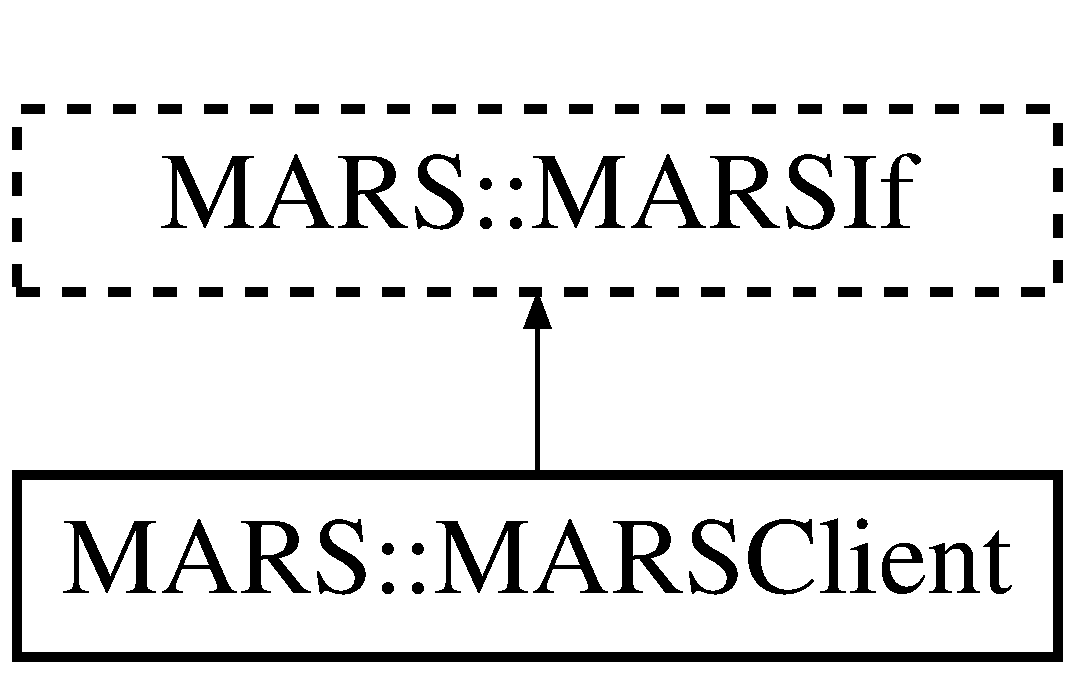
\includegraphics[height=2.000000cm]{classMARS_1_1MARSClient}
\end{center}
\end{figure}
\subsection*{Public Member Functions}
\begin{DoxyCompactItemize}
\item 
\mbox{\Hypertarget{classMARS_1_1MARSClient_af3edff1508e0791ed2f829b9cc8756dd}\label{classMARS_1_1MARSClient_af3edff1508e0791ed2f829b9cc8756dd}} 
{\bfseries M\+A\+R\+S\+Client} (boost\+::shared\+\_\+ptr$<$ \+::apache\+::thrift\+::protocol\+::\+T\+Protocol $>$ prot)
\item 
\mbox{\Hypertarget{classMARS_1_1MARSClient_acd3855458249e24c0296720d4abe3faa}\label{classMARS_1_1MARSClient_acd3855458249e24c0296720d4abe3faa}} 
{\bfseries M\+A\+R\+S\+Client} (boost\+::shared\+\_\+ptr$<$ \+::apache\+::thrift\+::protocol\+::\+T\+Protocol $>$ iprot, boost\+::shared\+\_\+ptr$<$ \+::apache\+::thrift\+::protocol\+::\+T\+Protocol $>$ oprot)
\item 
\mbox{\Hypertarget{classMARS_1_1MARSClient_a06872258392454e6ee5833faa07f03d2}\label{classMARS_1_1MARSClient_a06872258392454e6ee5833faa07f03d2}} 
boost\+::shared\+\_\+ptr$<$ \+::apache\+::thrift\+::protocol\+::\+T\+Protocol $>$ {\bfseries get\+Input\+Protocol} ()
\item 
\mbox{\Hypertarget{classMARS_1_1MARSClient_a71ef873ab97117877930a3698ae32dde}\label{classMARS_1_1MARSClient_a71ef873ab97117877930a3698ae32dde}} 
boost\+::shared\+\_\+ptr$<$ \+::apache\+::thrift\+::protocol\+::\+T\+Protocol $>$ {\bfseries get\+Output\+Protocol} ()
\item 
\mbox{\Hypertarget{classMARS_1_1MARSClient_ac23faa5a3a7debe8d0d3b58b2404ea9f}\label{classMARS_1_1MARSClient_ac23faa5a3a7debe8d0d3b58b2404ea9f}} 
void {\bfseries get\+Code} (std\+::string \&\+\_\+return)
\item 
\mbox{\Hypertarget{classMARS_1_1MARSClient_aec3947716605a8bf032e9dc326394ff8}\label{classMARS_1_1MARSClient_aec3947716605a8bf032e9dc326394ff8}} 
void {\bfseries send\+\_\+get\+Code} ()
\item 
\mbox{\Hypertarget{classMARS_1_1MARSClient_af274f93f5332375549a05604347a2492}\label{classMARS_1_1MARSClient_af274f93f5332375549a05604347a2492}} 
void {\bfseries recv\+\_\+get\+Code} (std\+::string \&\+\_\+return)
\item 
\mbox{\Hypertarget{classMARS_1_1MARSClient_a00caf56cd0ea03dfb4f40344c4052332}\label{classMARS_1_1MARSClient_a00caf56cd0ea03dfb4f40344c4052332}} 
void {\bfseries send\+Message} (std\+::string \&\+\_\+return)
\item 
\mbox{\Hypertarget{classMARS_1_1MARSClient_a86292876f325ea090b85fc1a50286636}\label{classMARS_1_1MARSClient_a86292876f325ea090b85fc1a50286636}} 
void {\bfseries send\+\_\+send\+Message} ()
\item 
\mbox{\Hypertarget{classMARS_1_1MARSClient_a9fae4d89950fea72ffb838afb1e6c1f8}\label{classMARS_1_1MARSClient_a9fae4d89950fea72ffb838afb1e6c1f8}} 
void {\bfseries recv\+\_\+send\+Message} (std\+::string \&\+\_\+return)
\item 
\mbox{\Hypertarget{classMARS_1_1MARSClient_a5b57bfe2de3bb1ac16f4bfb2f25ffad5}\label{classMARS_1_1MARSClient_a5b57bfe2de3bb1ac16f4bfb2f25ffad5}} 
void {\bfseries get\+Message} (const std\+::string \&message)
\item 
\mbox{\Hypertarget{classMARS_1_1MARSClient_a08dce57f389f3a1f1ad27b7425d64f25}\label{classMARS_1_1MARSClient_a08dce57f389f3a1f1ad27b7425d64f25}} 
void {\bfseries send\+\_\+get\+Message} (const std\+::string \&message)
\item 
\mbox{\Hypertarget{classMARS_1_1MARSClient_a60f109889c358359d552fd61a5204291}\label{classMARS_1_1MARSClient_a60f109889c358359d552fd61a5204291}} 
void {\bfseries recv\+\_\+get\+Message} ()
\item 
\mbox{\Hypertarget{classMARS_1_1MARSClient_ad1ed4cfa23ecdac579eb35b339d4e7d3}\label{classMARS_1_1MARSClient_ad1ed4cfa23ecdac579eb35b339d4e7d3}} 
void {\bfseries receive\+From\+JS} (const \hyperlink{classMARS_1_1Code}{Code} \&c)
\item 
\mbox{\Hypertarget{classMARS_1_1MARSClient_a2bf0b3fd8d3e859152f0e981f31be367}\label{classMARS_1_1MARSClient_a2bf0b3fd8d3e859152f0e981f31be367}} 
void {\bfseries send\+\_\+receive\+From\+JS} (const \hyperlink{classMARS_1_1Code}{Code} \&c)
\item 
\mbox{\Hypertarget{classMARS_1_1MARSClient_a20686999acd396aa67c614a92ea55a52}\label{classMARS_1_1MARSClient_a20686999acd396aa67c614a92ea55a52}} 
void {\bfseries recv\+\_\+receive\+From\+JS} ()
\item 
\mbox{\Hypertarget{classMARS_1_1MARSClient_a1415d9d072f05b14ff6c166fcaf6d73b}\label{classMARS_1_1MARSClient_a1415d9d072f05b14ff6c166fcaf6d73b}} 
void {\bfseries get\+Color\+Table} (std\+::vector$<$ std\+::string $>$ \&\+\_\+return)
\item 
\mbox{\Hypertarget{classMARS_1_1MARSClient_a9e1e350e8b588c329054e34868bd8622}\label{classMARS_1_1MARSClient_a9e1e350e8b588c329054e34868bd8622}} 
void {\bfseries send\+\_\+get\+Color\+Table} ()
\item 
\mbox{\Hypertarget{classMARS_1_1MARSClient_ab11a8a4cebac9a25ce1e5935c6ae4cff}\label{classMARS_1_1MARSClient_ab11a8a4cebac9a25ce1e5935c6ae4cff}} 
void {\bfseries recv\+\_\+get\+Color\+Table} (std\+::vector$<$ std\+::string $>$ \&\+\_\+return)
\item 
\mbox{\Hypertarget{classMARS_1_1MARSClient_a9c31b7e91c85e44ac6f5dfc211dcc8ee}\label{classMARS_1_1MARSClient_a9c31b7e91c85e44ac6f5dfc211dcc8ee}} 
void {\bfseries set\+Color\+Table} (const std\+::vector$<$ std\+::string $>$ \&color\+Table)
\item 
\mbox{\Hypertarget{classMARS_1_1MARSClient_a0ee2ae07f28bc4871d8cd8a7a5c5630b}\label{classMARS_1_1MARSClient_a0ee2ae07f28bc4871d8cd8a7a5c5630b}} 
void {\bfseries send\+\_\+set\+Color\+Table} (const std\+::vector$<$ std\+::string $>$ \&color\+Table)
\item 
\mbox{\Hypertarget{classMARS_1_1MARSClient_ae983c94389ce18d79d17d13e9ef8c6d9}\label{classMARS_1_1MARSClient_ae983c94389ce18d79d17d13e9ef8c6d9}} 
void {\bfseries recv\+\_\+set\+Color\+Table} ()
\end{DoxyCompactItemize}
\subsection*{Protected Attributes}
\begin{DoxyCompactItemize}
\item 
\mbox{\Hypertarget{classMARS_1_1MARSClient_a6748150d38d84ae1b6a6b75c00b37274}\label{classMARS_1_1MARSClient_a6748150d38d84ae1b6a6b75c00b37274}} 
boost\+::shared\+\_\+ptr$<$ \+::apache\+::thrift\+::protocol\+::\+T\+Protocol $>$ {\bfseries piprot\+\_\+}
\item 
\mbox{\Hypertarget{classMARS_1_1MARSClient_a0aa28c07742ed2a5770ffa46d2a21955}\label{classMARS_1_1MARSClient_a0aa28c07742ed2a5770ffa46d2a21955}} 
boost\+::shared\+\_\+ptr$<$ \+::apache\+::thrift\+::protocol\+::\+T\+Protocol $>$ {\bfseries poprot\+\_\+}
\item 
\mbox{\Hypertarget{classMARS_1_1MARSClient_adb00f31b62609abab17a40c5d80f2073}\label{classMARS_1_1MARSClient_adb00f31b62609abab17a40c5d80f2073}} 
\+::apache\+::thrift\+::protocol\+::\+T\+Protocol $\ast$ {\bfseries iprot\+\_\+}
\item 
\mbox{\Hypertarget{classMARS_1_1MARSClient_ac74389691d90dde0029d06a4e3d01553}\label{classMARS_1_1MARSClient_ac74389691d90dde0029d06a4e3d01553}} 
\+::apache\+::thrift\+::protocol\+::\+T\+Protocol $\ast$ {\bfseries oprot\+\_\+}
\end{DoxyCompactItemize}


The documentation for this class was generated from the following files\+:\begin{DoxyCompactItemize}
\item 
gen-\/cpp/M\+A\+R\+S.\+h\item 
gen-\/cpp/M\+A\+R\+S.\+cpp\end{DoxyCompactItemize}

\hypertarget{classMARS_1_1MARSConcurrentClient}{}\section{M\+A\+RS\+:\+:M\+A\+R\+S\+Concurrent\+Client Class Reference}
\label{classMARS_1_1MARSConcurrentClient}\index{M\+A\+R\+S\+::\+M\+A\+R\+S\+Concurrent\+Client@{M\+A\+R\+S\+::\+M\+A\+R\+S\+Concurrent\+Client}}
Inheritance diagram for M\+A\+RS\+:\+:M\+A\+R\+S\+Concurrent\+Client\+:\begin{figure}[H]
\begin{center}
\leavevmode
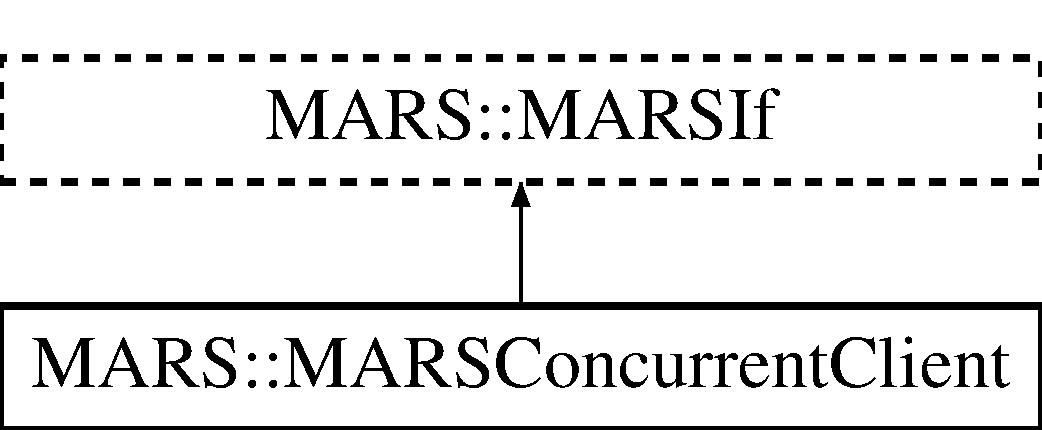
\includegraphics[height=2.000000cm]{classMARS_1_1MARSConcurrentClient}
\end{center}
\end{figure}
\subsection*{Public Member Functions}
\begin{DoxyCompactItemize}
\item 
\mbox{\Hypertarget{classMARS_1_1MARSConcurrentClient_a44e5432242b4a5aa4f8df5095ad31237}\label{classMARS_1_1MARSConcurrentClient_a44e5432242b4a5aa4f8df5095ad31237}} 
{\bfseries M\+A\+R\+S\+Concurrent\+Client} (boost\+::shared\+\_\+ptr$<$ \+::apache\+::thrift\+::protocol\+::\+T\+Protocol $>$ prot)
\item 
\mbox{\Hypertarget{classMARS_1_1MARSConcurrentClient_a03239381b801cca92980ba68830779a4}\label{classMARS_1_1MARSConcurrentClient_a03239381b801cca92980ba68830779a4}} 
{\bfseries M\+A\+R\+S\+Concurrent\+Client} (boost\+::shared\+\_\+ptr$<$ \+::apache\+::thrift\+::protocol\+::\+T\+Protocol $>$ iprot, boost\+::shared\+\_\+ptr$<$ \+::apache\+::thrift\+::protocol\+::\+T\+Protocol $>$ oprot)
\item 
\mbox{\Hypertarget{classMARS_1_1MARSConcurrentClient_ad5920bf681a05c34c72b8844ae42cc23}\label{classMARS_1_1MARSConcurrentClient_ad5920bf681a05c34c72b8844ae42cc23}} 
boost\+::shared\+\_\+ptr$<$ \+::apache\+::thrift\+::protocol\+::\+T\+Protocol $>$ {\bfseries get\+Input\+Protocol} ()
\item 
\mbox{\Hypertarget{classMARS_1_1MARSConcurrentClient_ae1a10971d664f7e69f9b08147426f18a}\label{classMARS_1_1MARSConcurrentClient_ae1a10971d664f7e69f9b08147426f18a}} 
boost\+::shared\+\_\+ptr$<$ \+::apache\+::thrift\+::protocol\+::\+T\+Protocol $>$ {\bfseries get\+Output\+Protocol} ()
\item 
\mbox{\Hypertarget{classMARS_1_1MARSConcurrentClient_a2791f9e0f7f4fbcf47805d7814fb58b3}\label{classMARS_1_1MARSConcurrentClient_a2791f9e0f7f4fbcf47805d7814fb58b3}} 
void {\bfseries get\+Code} (std\+::string \&\+\_\+return)
\item 
\mbox{\Hypertarget{classMARS_1_1MARSConcurrentClient_a4d92e8b570eedfd91e0c002a800bbf4f}\label{classMARS_1_1MARSConcurrentClient_a4d92e8b570eedfd91e0c002a800bbf4f}} 
int32\+\_\+t {\bfseries send\+\_\+get\+Code} ()
\item 
\mbox{\Hypertarget{classMARS_1_1MARSConcurrentClient_a7b99d43fe1efc59bbe811efe1074902e}\label{classMARS_1_1MARSConcurrentClient_a7b99d43fe1efc59bbe811efe1074902e}} 
void {\bfseries recv\+\_\+get\+Code} (std\+::string \&\+\_\+return, const int32\+\_\+t seqid)
\item 
\mbox{\Hypertarget{classMARS_1_1MARSConcurrentClient_a8bf493c19377e69e01fc94b40b758184}\label{classMARS_1_1MARSConcurrentClient_a8bf493c19377e69e01fc94b40b758184}} 
void {\bfseries send\+Message} (std\+::string \&\+\_\+return)
\item 
\mbox{\Hypertarget{classMARS_1_1MARSConcurrentClient_a7dca0094b73698f263fb6f6201e5520b}\label{classMARS_1_1MARSConcurrentClient_a7dca0094b73698f263fb6f6201e5520b}} 
int32\+\_\+t {\bfseries send\+\_\+send\+Message} ()
\item 
\mbox{\Hypertarget{classMARS_1_1MARSConcurrentClient_a29d26ae66c87a412666bb37366adfd80}\label{classMARS_1_1MARSConcurrentClient_a29d26ae66c87a412666bb37366adfd80}} 
void {\bfseries recv\+\_\+send\+Message} (std\+::string \&\+\_\+return, const int32\+\_\+t seqid)
\item 
\mbox{\Hypertarget{classMARS_1_1MARSConcurrentClient_a512bea2e51a5af96d0400de8212f5e78}\label{classMARS_1_1MARSConcurrentClient_a512bea2e51a5af96d0400de8212f5e78}} 
void {\bfseries get\+Message} (const std\+::string \&message)
\item 
\mbox{\Hypertarget{classMARS_1_1MARSConcurrentClient_a5df674de5c9b907d883ca6c83c9f362a}\label{classMARS_1_1MARSConcurrentClient_a5df674de5c9b907d883ca6c83c9f362a}} 
int32\+\_\+t {\bfseries send\+\_\+get\+Message} (const std\+::string \&message)
\item 
\mbox{\Hypertarget{classMARS_1_1MARSConcurrentClient_a6864176227e2850d6f8b1e4e744cda72}\label{classMARS_1_1MARSConcurrentClient_a6864176227e2850d6f8b1e4e744cda72}} 
void {\bfseries recv\+\_\+get\+Message} (const int32\+\_\+t seqid)
\item 
\mbox{\Hypertarget{classMARS_1_1MARSConcurrentClient_af1b867b5428d8b73b12b579ef92b1abe}\label{classMARS_1_1MARSConcurrentClient_af1b867b5428d8b73b12b579ef92b1abe}} 
void {\bfseries receive\+From\+JS} (const \hyperlink{classMARS_1_1Code}{Code} \&c)
\item 
\mbox{\Hypertarget{classMARS_1_1MARSConcurrentClient_a1c4f8d29e9b16f96961232ad5d190e95}\label{classMARS_1_1MARSConcurrentClient_a1c4f8d29e9b16f96961232ad5d190e95}} 
int32\+\_\+t {\bfseries send\+\_\+receive\+From\+JS} (const \hyperlink{classMARS_1_1Code}{Code} \&c)
\item 
\mbox{\Hypertarget{classMARS_1_1MARSConcurrentClient_ac03c1465036104325f70dd7b90b7d65e}\label{classMARS_1_1MARSConcurrentClient_ac03c1465036104325f70dd7b90b7d65e}} 
void {\bfseries recv\+\_\+receive\+From\+JS} (const int32\+\_\+t seqid)
\item 
\mbox{\Hypertarget{classMARS_1_1MARSConcurrentClient_a6e1a523f7b3f7a86fc6c7e441072f7ef}\label{classMARS_1_1MARSConcurrentClient_a6e1a523f7b3f7a86fc6c7e441072f7ef}} 
void {\bfseries get\+Color\+Table} (std\+::vector$<$ std\+::string $>$ \&\+\_\+return)
\item 
\mbox{\Hypertarget{classMARS_1_1MARSConcurrentClient_a3d8e8c14814bc75a56b0d44e4a64b630}\label{classMARS_1_1MARSConcurrentClient_a3d8e8c14814bc75a56b0d44e4a64b630}} 
int32\+\_\+t {\bfseries send\+\_\+get\+Color\+Table} ()
\item 
\mbox{\Hypertarget{classMARS_1_1MARSConcurrentClient_ac9b85a17f818f274c012526f55c6b63f}\label{classMARS_1_1MARSConcurrentClient_ac9b85a17f818f274c012526f55c6b63f}} 
void {\bfseries recv\+\_\+get\+Color\+Table} (std\+::vector$<$ std\+::string $>$ \&\+\_\+return, const int32\+\_\+t seqid)
\item 
\mbox{\Hypertarget{classMARS_1_1MARSConcurrentClient_a30ab9c7af1f8004627f5b3dd7c3d708d}\label{classMARS_1_1MARSConcurrentClient_a30ab9c7af1f8004627f5b3dd7c3d708d}} 
void {\bfseries set\+Color\+Table} (const std\+::vector$<$ std\+::string $>$ \&color\+Table)
\item 
\mbox{\Hypertarget{classMARS_1_1MARSConcurrentClient_a25e1d52136ba48a6ab36dcdb26f96992}\label{classMARS_1_1MARSConcurrentClient_a25e1d52136ba48a6ab36dcdb26f96992}} 
int32\+\_\+t {\bfseries send\+\_\+set\+Color\+Table} (const std\+::vector$<$ std\+::string $>$ \&color\+Table)
\item 
\mbox{\Hypertarget{classMARS_1_1MARSConcurrentClient_aaf2eb6886251ebd58e09bbba02566c5a}\label{classMARS_1_1MARSConcurrentClient_aaf2eb6886251ebd58e09bbba02566c5a}} 
void {\bfseries recv\+\_\+set\+Color\+Table} (const int32\+\_\+t seqid)
\end{DoxyCompactItemize}
\subsection*{Protected Attributes}
\begin{DoxyCompactItemize}
\item 
\mbox{\Hypertarget{classMARS_1_1MARSConcurrentClient_abbc464f5cd88899e7b55b365b8999c14}\label{classMARS_1_1MARSConcurrentClient_abbc464f5cd88899e7b55b365b8999c14}} 
boost\+::shared\+\_\+ptr$<$ \+::apache\+::thrift\+::protocol\+::\+T\+Protocol $>$ {\bfseries piprot\+\_\+}
\item 
\mbox{\Hypertarget{classMARS_1_1MARSConcurrentClient_a41f7e0d838a100400b56cc5763f5bf40}\label{classMARS_1_1MARSConcurrentClient_a41f7e0d838a100400b56cc5763f5bf40}} 
boost\+::shared\+\_\+ptr$<$ \+::apache\+::thrift\+::protocol\+::\+T\+Protocol $>$ {\bfseries poprot\+\_\+}
\item 
\mbox{\Hypertarget{classMARS_1_1MARSConcurrentClient_a7b6a397647c0f402fd48b8167afa3a97}\label{classMARS_1_1MARSConcurrentClient_a7b6a397647c0f402fd48b8167afa3a97}} 
\+::apache\+::thrift\+::protocol\+::\+T\+Protocol $\ast$ {\bfseries iprot\+\_\+}
\item 
\mbox{\Hypertarget{classMARS_1_1MARSConcurrentClient_aca981420dbb6290f7ede939b6e5e65a5}\label{classMARS_1_1MARSConcurrentClient_aca981420dbb6290f7ede939b6e5e65a5}} 
\+::apache\+::thrift\+::protocol\+::\+T\+Protocol $\ast$ {\bfseries oprot\+\_\+}
\item 
\mbox{\Hypertarget{classMARS_1_1MARSConcurrentClient_a795ec38fc8ea43d932d8de438d2a3678}\label{classMARS_1_1MARSConcurrentClient_a795ec38fc8ea43d932d8de438d2a3678}} 
\+::apache\+::thrift\+::async\+::\+T\+Concurrent\+Client\+Sync\+Info {\bfseries sync\+\_\+}
\end{DoxyCompactItemize}


The documentation for this class was generated from the following files\+:\begin{DoxyCompactItemize}
\item 
gen-\/cpp/M\+A\+R\+S.\+h\item 
gen-\/cpp/M\+A\+R\+S.\+cpp\end{DoxyCompactItemize}

\hypertarget{classMARS_1_1marsConstants}{}\section{M\+A\+RS\+:\+:mars\+Constants Class Reference}
\label{classMARS_1_1marsConstants}\index{M\+A\+R\+S\+::mars\+Constants@{M\+A\+R\+S\+::mars\+Constants}}


The documentation for this class was generated from the following files\+:\begin{DoxyCompactItemize}
\item 
gen-\/cpp/mars\+\_\+constants.\+h\item 
gen-\/cpp/mars\+\_\+constants.\+cpp\end{DoxyCompactItemize}

\hypertarget{classMarsEngine}{}\section{Mars\+Engine Class Reference}
\label{classMarsEngine}\index{Mars\+Engine@{Mars\+Engine}}
\subsection*{Public Member Functions}
\begin{DoxyCompactItemize}
\item 
\mbox{\Hypertarget{classMarsEngine_a39ad8b0376b8032cb4abd6e32394b649}\label{classMarsEngine_a39ad8b0376b8032cb4abd6e32394b649}} 
std\+::shared\+\_\+ptr$<$ \hyperlink{classOperationParams}{Operation\+Params} $>$ {\bfseries execute} (\hyperlink{classMemoryIndex}{Memory\+Index} m\+Index)
\item 
\mbox{\Hypertarget{classMarsEngine_ae987f2993dc6716a2ecbff8161c321b6}\label{classMarsEngine_ae987f2993dc6716a2ecbff8161c321b6}} 
const std\+::vector$<$ \hyperlink{classInstruction}{Instruction} $>$ {\bfseries get\+Memory\+Array} ()
\item 
\mbox{\Hypertarget{classMarsEngine_afca3d92f704360f86ce5e0d588fbb0e3}\label{classMarsEngine_afca3d92f704360f86ce5e0d588fbb0e3}} 
void {\bfseries enter\+Warrior} (int begin\+Addres, std\+::vector$<$ \hyperlink{classInstruction}{Instruction} $>$ code)
\item 
\mbox{\Hypertarget{classMarsEngine_aad6972df3bbd3f9d1c4278d7b5cd51d0}\label{classMarsEngine_aad6972df3bbd3f9d1c4278d7b5cd51d0}} 
std\+::shared\+\_\+ptr$<$ \hyperlink{classMarsOperation}{Mars\+Operation} $>$ {\bfseries get\+Operation} (\hyperlink{classMemoryIndex}{Memory\+Index} index)
\end{DoxyCompactItemize}


The documentation for this class was generated from the following files\+:\begin{DoxyCompactItemize}
\item 
logic/mars/Mars\+Engine.\+h\item 
logic/mars/Mars\+Engine.\+cpp\end{DoxyCompactItemize}

\hypertarget{classMARSHandler}{}\section{M\+A\+R\+S\+Handler Class Reference}
\label{classMARSHandler}\index{M\+A\+R\+S\+Handler@{M\+A\+R\+S\+Handler}}
Inheritance diagram for M\+A\+R\+S\+Handler\+:\begin{figure}[H]
\begin{center}
\leavevmode
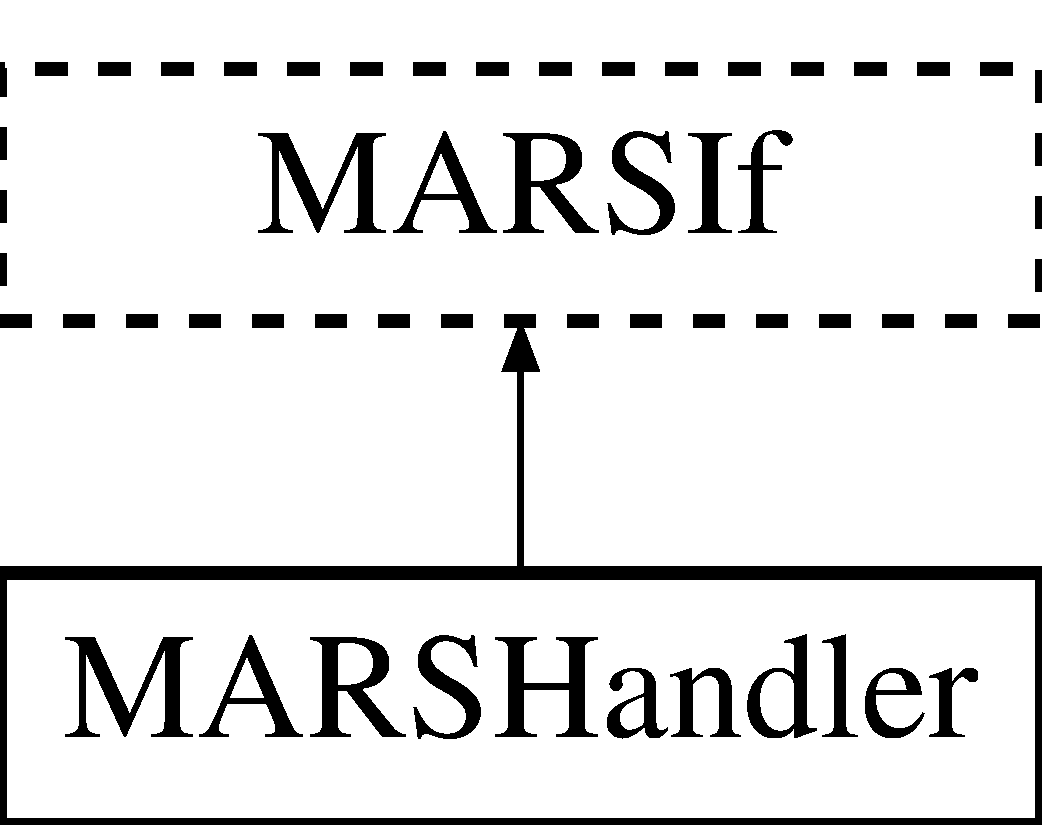
\includegraphics[height=2.000000cm]{classMARSHandler}
\end{center}
\end{figure}
\subsection*{Public Member Functions}
\begin{DoxyCompactItemize}
\item 
void \hyperlink{classMARSHandler_aad361446a8dab85013f8eea681c95663}{receive\+From\+JS} (const Code \&c)
\item 
void \hyperlink{classMARSHandler_a59f960d2b59109d22eb25911284c167c}{send\+Message} (std\+::string \&\+\_\+return)
\item 
void \hyperlink{classMARSHandler_a87dbdc238b461bf59eb53e0a881aa34e}{get\+Message} (const std\+::string \&message)
\item 
void \hyperlink{classMARSHandler_a051b0a327d012bebb315083e5faf80e4}{get\+Code} (std\+::string \&\+\_\+return)
\item 
void \hyperlink{classMARSHandler_a9cc24026adecda320622810448188173}{get\+Color\+Table} (std\+::vector$<$ std\+::string $>$ \&\+\_\+return)
\item 
void \hyperlink{classMARSHandler_ac332bb9228000d1220fe80366fbccea4}{set\+Color\+Table} (const std\+::vector$<$ std\+::string $>$ \&color\+Table)
\end{DoxyCompactItemize}


\subsection{Member Function Documentation}
\mbox{\Hypertarget{classMARSHandler_a051b0a327d012bebb315083e5faf80e4}\label{classMARSHandler_a051b0a327d012bebb315083e5faf80e4}} 
\index{M\+A\+R\+S\+Handler@{M\+A\+R\+S\+Handler}!get\+Code@{get\+Code}}
\index{get\+Code@{get\+Code}!M\+A\+R\+S\+Handler@{M\+A\+R\+S\+Handler}}
\subsubsection{\texorpdfstring{get\+Code()}{getCode()}}
{\footnotesize\ttfamily void M\+A\+R\+S\+Handler\+::get\+Code (\begin{DoxyParamCaption}\item[{std\+::string \&}]{\+\_\+return }\end{DoxyParamCaption})\hspace{0.3cm}{\ttfamily [inline]}}

Send code from javascript to c++ client 
\begin{DoxyParams}{Parameters}
{\em \+\_\+return} & player\textquotesingle{}s code \\
\hline
\end{DoxyParams}
\mbox{\Hypertarget{classMARSHandler_a9cc24026adecda320622810448188173}\label{classMARSHandler_a9cc24026adecda320622810448188173}} 
\index{M\+A\+R\+S\+Handler@{M\+A\+R\+S\+Handler}!get\+Color\+Table@{get\+Color\+Table}}
\index{get\+Color\+Table@{get\+Color\+Table}!M\+A\+R\+S\+Handler@{M\+A\+R\+S\+Handler}}
\subsubsection{\texorpdfstring{get\+Color\+Table()}{getColorTable()}}
{\footnotesize\ttfamily void M\+A\+R\+S\+Handler\+::get\+Color\+Table (\begin{DoxyParamCaption}\item[{std\+::vector$<$ std\+::string $>$ \&}]{\+\_\+return }\end{DoxyParamCaption})\hspace{0.3cm}{\ttfamily [inline]}}

Send vector with colors to draw to javascript 
\begin{DoxyParams}{Parameters}
{\em \+\_\+return} & table with colors \\
\hline
\end{DoxyParams}
\mbox{\Hypertarget{classMARSHandler_a87dbdc238b461bf59eb53e0a881aa34e}\label{classMARSHandler_a87dbdc238b461bf59eb53e0a881aa34e}} 
\index{M\+A\+R\+S\+Handler@{M\+A\+R\+S\+Handler}!get\+Message@{get\+Message}}
\index{get\+Message@{get\+Message}!M\+A\+R\+S\+Handler@{M\+A\+R\+S\+Handler}}
\subsubsection{\texorpdfstring{get\+Message()}{getMessage()}}
{\footnotesize\ttfamily void M\+A\+R\+S\+Handler\+::get\+Message (\begin{DoxyParamCaption}\item[{const std\+::string \&}]{message }\end{DoxyParamCaption})\hspace{0.3cm}{\ttfamily [inline]}}

Receive message from c++ client whether parsing succeeded 
\begin{DoxyParams}{Parameters}
{\em message} & \\
\hline
\end{DoxyParams}
\mbox{\Hypertarget{classMARSHandler_aad361446a8dab85013f8eea681c95663}\label{classMARSHandler_aad361446a8dab85013f8eea681c95663}} 
\index{M\+A\+R\+S\+Handler@{M\+A\+R\+S\+Handler}!receive\+From\+JS@{receive\+From\+JS}}
\index{receive\+From\+JS@{receive\+From\+JS}!M\+A\+R\+S\+Handler@{M\+A\+R\+S\+Handler}}
\subsubsection{\texorpdfstring{receive\+From\+J\+S()}{receiveFromJS()}}
{\footnotesize\ttfamily void M\+A\+R\+S\+Handler\+::receive\+From\+JS (\begin{DoxyParamCaption}\item[{const Code \&}]{c }\end{DoxyParamCaption})\hspace{0.3cm}{\ttfamily [inline]}}

Get redcode from browser 
\begin{DoxyParams}{Parameters}
{\em c} & structure containing player\textquotesingle{}s code \\
\hline
\end{DoxyParams}
\mbox{\Hypertarget{classMARSHandler_a59f960d2b59109d22eb25911284c167c}\label{classMARSHandler_a59f960d2b59109d22eb25911284c167c}} 
\index{M\+A\+R\+S\+Handler@{M\+A\+R\+S\+Handler}!send\+Message@{send\+Message}}
\index{send\+Message@{send\+Message}!M\+A\+R\+S\+Handler@{M\+A\+R\+S\+Handler}}
\subsubsection{\texorpdfstring{send\+Message()}{sendMessage()}}
{\footnotesize\ttfamily void M\+A\+R\+S\+Handler\+::send\+Message (\begin{DoxyParamCaption}\item[{std\+::string \&}]{\+\_\+return }\end{DoxyParamCaption})\hspace{0.3cm}{\ttfamily [inline]}}

Tell javascript if code parsing succeeded or not 
\begin{DoxyParams}{Parameters}
{\em \+\_\+return} & message sent to javascript \\
\hline
\end{DoxyParams}
\mbox{\Hypertarget{classMARSHandler_ac332bb9228000d1220fe80366fbccea4}\label{classMARSHandler_ac332bb9228000d1220fe80366fbccea4}} 
\index{M\+A\+R\+S\+Handler@{M\+A\+R\+S\+Handler}!set\+Color\+Table@{set\+Color\+Table}}
\index{set\+Color\+Table@{set\+Color\+Table}!M\+A\+R\+S\+Handler@{M\+A\+R\+S\+Handler}}
\subsubsection{\texorpdfstring{set\+Color\+Table()}{setColorTable()}}
{\footnotesize\ttfamily void M\+A\+R\+S\+Handler\+::set\+Color\+Table (\begin{DoxyParamCaption}\item[{const std\+::vector$<$ std\+::string $>$ \&}]{color\+Table }\end{DoxyParamCaption})\hspace{0.3cm}{\ttfamily [inline]}}

Receive vector with colors from c++ client 
\begin{DoxyParams}{Parameters}
{\em color\+Table} & \\
\hline
\end{DoxyParams}


The documentation for this class was generated from the following file\+:\begin{DoxyCompactItemize}
\item 
server/server.\+cpp\end{DoxyCompactItemize}

\hypertarget{classMARS_1_1MARSIf}{}\section{M\+A\+RS\+:\+:M\+A\+R\+S\+If Class Reference}
\label{classMARS_1_1MARSIf}\index{M\+A\+R\+S\+::\+M\+A\+R\+S\+If@{M\+A\+R\+S\+::\+M\+A\+R\+S\+If}}
Inheritance diagram for M\+A\+RS\+:\+:M\+A\+R\+S\+If\+:\begin{figure}[H]
\begin{center}
\leavevmode
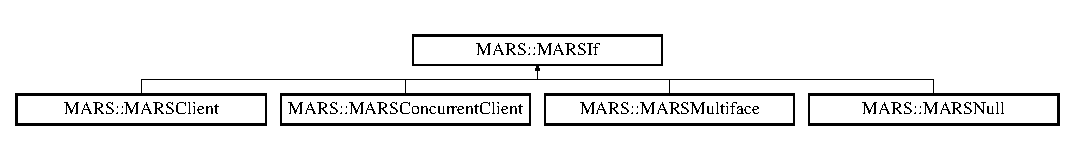
\includegraphics[height=1.443299cm]{classMARS_1_1MARSIf}
\end{center}
\end{figure}
\subsection*{Public Member Functions}
\begin{DoxyCompactItemize}
\item 
\mbox{\Hypertarget{classMARS_1_1MARSIf_ad9000319d6abe1db975c438b2988c20a}\label{classMARS_1_1MARSIf_ad9000319d6abe1db975c438b2988c20a}} 
virtual void {\bfseries get\+Code} (std\+::string \&\+\_\+return)=0
\item 
\mbox{\Hypertarget{classMARS_1_1MARSIf_a48804756c1d66c67d7275145d9c0b723}\label{classMARS_1_1MARSIf_a48804756c1d66c67d7275145d9c0b723}} 
virtual void {\bfseries send\+Message} (std\+::string \&\+\_\+return)=0
\item 
\mbox{\Hypertarget{classMARS_1_1MARSIf_a59082cb21aa687137f8a4e18ee4e802b}\label{classMARS_1_1MARSIf_a59082cb21aa687137f8a4e18ee4e802b}} 
virtual void {\bfseries get\+Message} (const std\+::string \&message)=0
\item 
\mbox{\Hypertarget{classMARS_1_1MARSIf_a72146cab12d00c5ca1e7bd68d7548e8c}\label{classMARS_1_1MARSIf_a72146cab12d00c5ca1e7bd68d7548e8c}} 
virtual void {\bfseries receive\+From\+JS} (const \hyperlink{classMARS_1_1Code}{Code} \&c)=0
\item 
\mbox{\Hypertarget{classMARS_1_1MARSIf_af643a67825196fc9c659ea04bd892b17}\label{classMARS_1_1MARSIf_af643a67825196fc9c659ea04bd892b17}} 
virtual void {\bfseries get\+Color\+Table} (std\+::vector$<$ std\+::string $>$ \&\+\_\+return)=0
\item 
\mbox{\Hypertarget{classMARS_1_1MARSIf_a3aae6af9e5828e00a2da6316728b0cbb}\label{classMARS_1_1MARSIf_a3aae6af9e5828e00a2da6316728b0cbb}} 
virtual void {\bfseries set\+Color\+Table} (const std\+::vector$<$ std\+::string $>$ \&color\+Table)=0
\end{DoxyCompactItemize}


The documentation for this class was generated from the following file\+:\begin{DoxyCompactItemize}
\item 
gen-\/cpp/M\+A\+R\+S.\+h\end{DoxyCompactItemize}

\hypertarget{classMARS_1_1MARSIfFactory}{}\section{M\+A\+RS\+:\+:M\+A\+R\+S\+If\+Factory Class Reference}
\label{classMARS_1_1MARSIfFactory}\index{M\+A\+R\+S\+::\+M\+A\+R\+S\+If\+Factory@{M\+A\+R\+S\+::\+M\+A\+R\+S\+If\+Factory}}
Inheritance diagram for M\+A\+RS\+:\+:M\+A\+R\+S\+If\+Factory\+:\begin{figure}[H]
\begin{center}
\leavevmode
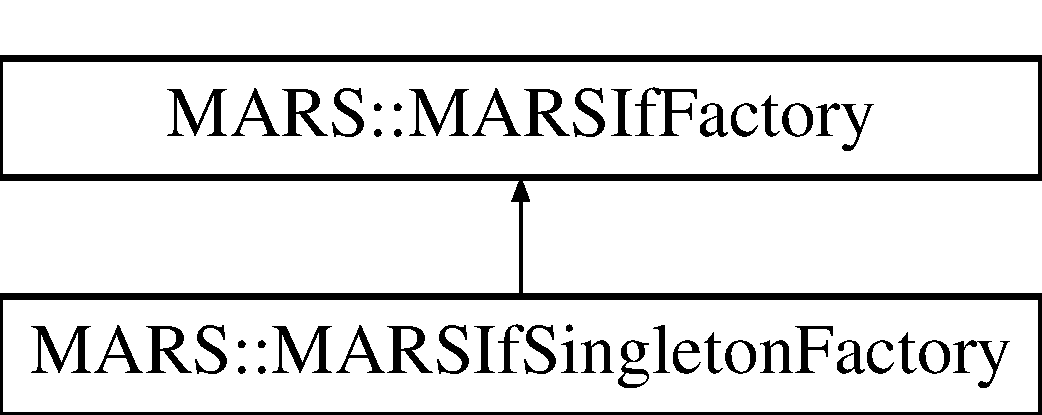
\includegraphics[height=2.000000cm]{classMARS_1_1MARSIfFactory}
\end{center}
\end{figure}
\subsection*{Public Types}
\begin{DoxyCompactItemize}
\item 
\mbox{\Hypertarget{classMARS_1_1MARSIfFactory_aa263d8e893e274c43576ad71255ead2a}\label{classMARS_1_1MARSIfFactory_aa263d8e893e274c43576ad71255ead2a}} 
typedef \hyperlink{classMARS_1_1MARSIf}{M\+A\+R\+S\+If} {\bfseries Handler}
\end{DoxyCompactItemize}
\subsection*{Public Member Functions}
\begin{DoxyCompactItemize}
\item 
\mbox{\Hypertarget{classMARS_1_1MARSIfFactory_a6e93aa23111ebd1156e2f3900b3105da}\label{classMARS_1_1MARSIfFactory_a6e93aa23111ebd1156e2f3900b3105da}} 
virtual \hyperlink{classMARS_1_1MARSIf}{M\+A\+R\+S\+If} $\ast$ {\bfseries get\+Handler} (const \+::apache\+::thrift\+::\+T\+Connection\+Info \&conn\+Info)=0
\item 
\mbox{\Hypertarget{classMARS_1_1MARSIfFactory_a4e6ba812f3ec56383d55ff469b95da1e}\label{classMARS_1_1MARSIfFactory_a4e6ba812f3ec56383d55ff469b95da1e}} 
virtual void {\bfseries release\+Handler} (\hyperlink{classMARS_1_1MARSIf}{M\+A\+R\+S\+If} $\ast$)=0
\end{DoxyCompactItemize}


The documentation for this class was generated from the following file\+:\begin{DoxyCompactItemize}
\item 
gen-\/cpp/M\+A\+R\+S.\+h\end{DoxyCompactItemize}

\hypertarget{classMARS_1_1MARSIfSingletonFactory}{}\section{M\+A\+RS\+:\+:M\+A\+R\+S\+If\+Singleton\+Factory Class Reference}
\label{classMARS_1_1MARSIfSingletonFactory}\index{M\+A\+R\+S\+::\+M\+A\+R\+S\+If\+Singleton\+Factory@{M\+A\+R\+S\+::\+M\+A\+R\+S\+If\+Singleton\+Factory}}
Inheritance diagram for M\+A\+RS\+:\+:M\+A\+R\+S\+If\+Singleton\+Factory\+:\begin{figure}[H]
\begin{center}
\leavevmode
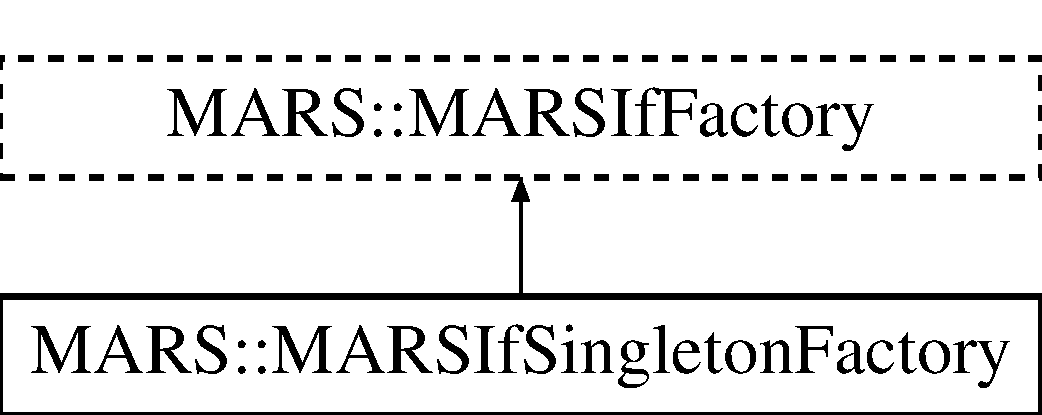
\includegraphics[height=2.000000cm]{classMARS_1_1MARSIfSingletonFactory}
\end{center}
\end{figure}
\subsection*{Public Member Functions}
\begin{DoxyCompactItemize}
\item 
\mbox{\Hypertarget{classMARS_1_1MARSIfSingletonFactory_abdd13d59a2258721e7d9056ef9725e02}\label{classMARS_1_1MARSIfSingletonFactory_abdd13d59a2258721e7d9056ef9725e02}} 
{\bfseries M\+A\+R\+S\+If\+Singleton\+Factory} (const boost\+::shared\+\_\+ptr$<$ \hyperlink{classMARS_1_1MARSIf}{M\+A\+R\+S\+If} $>$ \&iface)
\item 
\mbox{\Hypertarget{classMARS_1_1MARSIfSingletonFactory_a50b150cc2ad9a9667dee2450358eda3b}\label{classMARS_1_1MARSIfSingletonFactory_a50b150cc2ad9a9667dee2450358eda3b}} 
virtual \hyperlink{classMARS_1_1MARSIf}{M\+A\+R\+S\+If} $\ast$ {\bfseries get\+Handler} (const \+::apache\+::thrift\+::\+T\+Connection\+Info \&)
\item 
\mbox{\Hypertarget{classMARS_1_1MARSIfSingletonFactory_a4ac0f81061299ec902ca2846ee18f6e4}\label{classMARS_1_1MARSIfSingletonFactory_a4ac0f81061299ec902ca2846ee18f6e4}} 
virtual void {\bfseries release\+Handler} (\hyperlink{classMARS_1_1MARSIf}{M\+A\+R\+S\+If} $\ast$)
\end{DoxyCompactItemize}
\subsection*{Protected Attributes}
\begin{DoxyCompactItemize}
\item 
\mbox{\Hypertarget{classMARS_1_1MARSIfSingletonFactory_afc72e008c138f691860d12d20768ac77}\label{classMARS_1_1MARSIfSingletonFactory_afc72e008c138f691860d12d20768ac77}} 
boost\+::shared\+\_\+ptr$<$ \hyperlink{classMARS_1_1MARSIf}{M\+A\+R\+S\+If} $>$ {\bfseries iface\+\_\+}
\end{DoxyCompactItemize}
\subsection*{Additional Inherited Members}


The documentation for this class was generated from the following file\+:\begin{DoxyCompactItemize}
\item 
gen-\/cpp/M\+A\+R\+S.\+h\end{DoxyCompactItemize}

\hypertarget{classMARS_1_1MARSMultiface}{}\section{M\+A\+RS\+:\+:M\+A\+R\+S\+Multiface Class Reference}
\label{classMARS_1_1MARSMultiface}\index{M\+A\+R\+S\+::\+M\+A\+R\+S\+Multiface@{M\+A\+R\+S\+::\+M\+A\+R\+S\+Multiface}}
Inheritance diagram for M\+A\+RS\+:\+:M\+A\+R\+S\+Multiface\+:\begin{figure}[H]
\begin{center}
\leavevmode
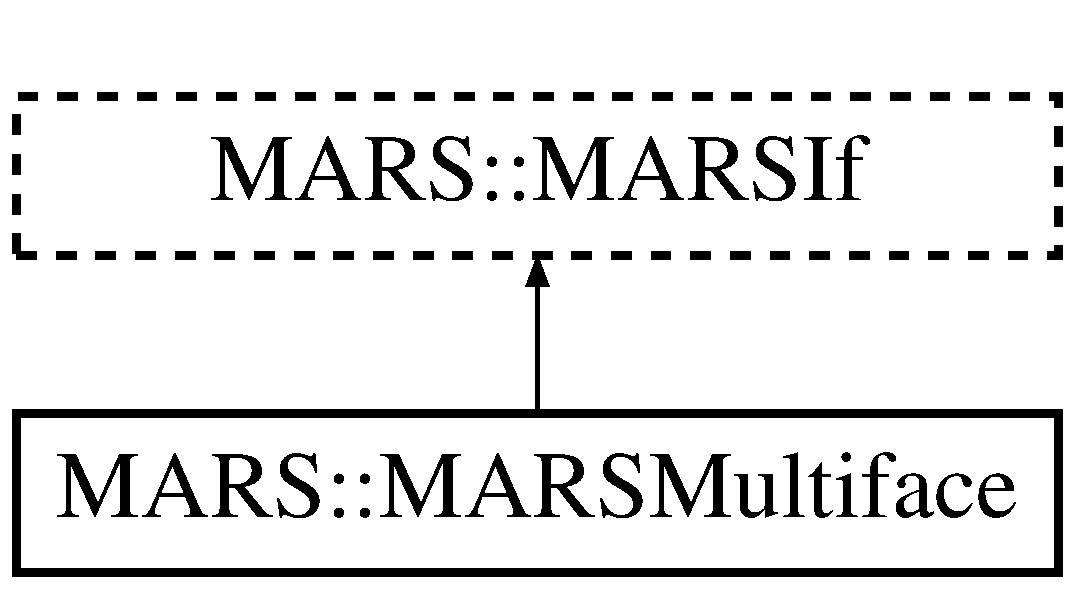
\includegraphics[height=2.000000cm]{classMARS_1_1MARSMultiface}
\end{center}
\end{figure}
\subsection*{Public Member Functions}
\begin{DoxyCompactItemize}
\item 
\mbox{\Hypertarget{classMARS_1_1MARSMultiface_a887e7159fba8bf9c71e49eb537c74722}\label{classMARS_1_1MARSMultiface_a887e7159fba8bf9c71e49eb537c74722}} 
{\bfseries M\+A\+R\+S\+Multiface} (std\+::vector$<$ boost\+::shared\+\_\+ptr$<$ \hyperlink{classMARS_1_1MARSIf}{M\+A\+R\+S\+If} $>$ $>$ \&ifaces)
\item 
\mbox{\Hypertarget{classMARS_1_1MARSMultiface_a2536d45efd4861530b4de8ad4a6741e2}\label{classMARS_1_1MARSMultiface_a2536d45efd4861530b4de8ad4a6741e2}} 
void {\bfseries get\+Code} (std\+::string \&\+\_\+return)
\item 
\mbox{\Hypertarget{classMARS_1_1MARSMultiface_af6152624ee8ebb1885c8ea941ff6a50c}\label{classMARS_1_1MARSMultiface_af6152624ee8ebb1885c8ea941ff6a50c}} 
void {\bfseries send\+Message} (std\+::string \&\+\_\+return)
\item 
\mbox{\Hypertarget{classMARS_1_1MARSMultiface_a83560afc009f11281238af7f00e483a4}\label{classMARS_1_1MARSMultiface_a83560afc009f11281238af7f00e483a4}} 
void {\bfseries get\+Message} (const std\+::string \&message)
\item 
\mbox{\Hypertarget{classMARS_1_1MARSMultiface_a2c514419a0c3eeba1336fb7aaac4bdda}\label{classMARS_1_1MARSMultiface_a2c514419a0c3eeba1336fb7aaac4bdda}} 
void {\bfseries receive\+From\+JS} (const \hyperlink{classMARS_1_1Code}{Code} \&c)
\item 
\mbox{\Hypertarget{classMARS_1_1MARSMultiface_ad1fd464ed427ca30b3fcb7cc5e40b53f}\label{classMARS_1_1MARSMultiface_ad1fd464ed427ca30b3fcb7cc5e40b53f}} 
void {\bfseries get\+Color\+Table} (std\+::vector$<$ std\+::string $>$ \&\+\_\+return)
\item 
\mbox{\Hypertarget{classMARS_1_1MARSMultiface_a4849eaef827f6dfb4cbac9697da697d5}\label{classMARS_1_1MARSMultiface_a4849eaef827f6dfb4cbac9697da697d5}} 
void {\bfseries set\+Color\+Table} (const std\+::vector$<$ std\+::string $>$ \&color\+Table)
\end{DoxyCompactItemize}
\subsection*{Protected Member Functions}
\begin{DoxyCompactItemize}
\item 
\mbox{\Hypertarget{classMARS_1_1MARSMultiface_a3af2c2f1319f8c37e6aacfe87e4d7c5b}\label{classMARS_1_1MARSMultiface_a3af2c2f1319f8c37e6aacfe87e4d7c5b}} 
void {\bfseries add} (boost\+::shared\+\_\+ptr$<$ \hyperlink{classMARS_1_1MARSIf}{M\+A\+R\+S\+If} $>$ iface)
\end{DoxyCompactItemize}
\subsection*{Protected Attributes}
\begin{DoxyCompactItemize}
\item 
\mbox{\Hypertarget{classMARS_1_1MARSMultiface_a1de93b18505fbdf11175313509f40b7b}\label{classMARS_1_1MARSMultiface_a1de93b18505fbdf11175313509f40b7b}} 
std\+::vector$<$ boost\+::shared\+\_\+ptr$<$ \hyperlink{classMARS_1_1MARSIf}{M\+A\+R\+S\+If} $>$ $>$ {\bfseries ifaces\+\_\+}
\end{DoxyCompactItemize}


The documentation for this class was generated from the following file\+:\begin{DoxyCompactItemize}
\item 
gen-\/cpp/M\+A\+R\+S.\+h\end{DoxyCompactItemize}

\hypertarget{classMARS_1_1MARSNull}{}\section{M\+A\+RS\+:\+:M\+A\+R\+S\+Null Class Reference}
\label{classMARS_1_1MARSNull}\index{M\+A\+R\+S\+::\+M\+A\+R\+S\+Null@{M\+A\+R\+S\+::\+M\+A\+R\+S\+Null}}
Inheritance diagram for M\+A\+RS\+:\+:M\+A\+R\+S\+Null\+:\begin{figure}[H]
\begin{center}
\leavevmode
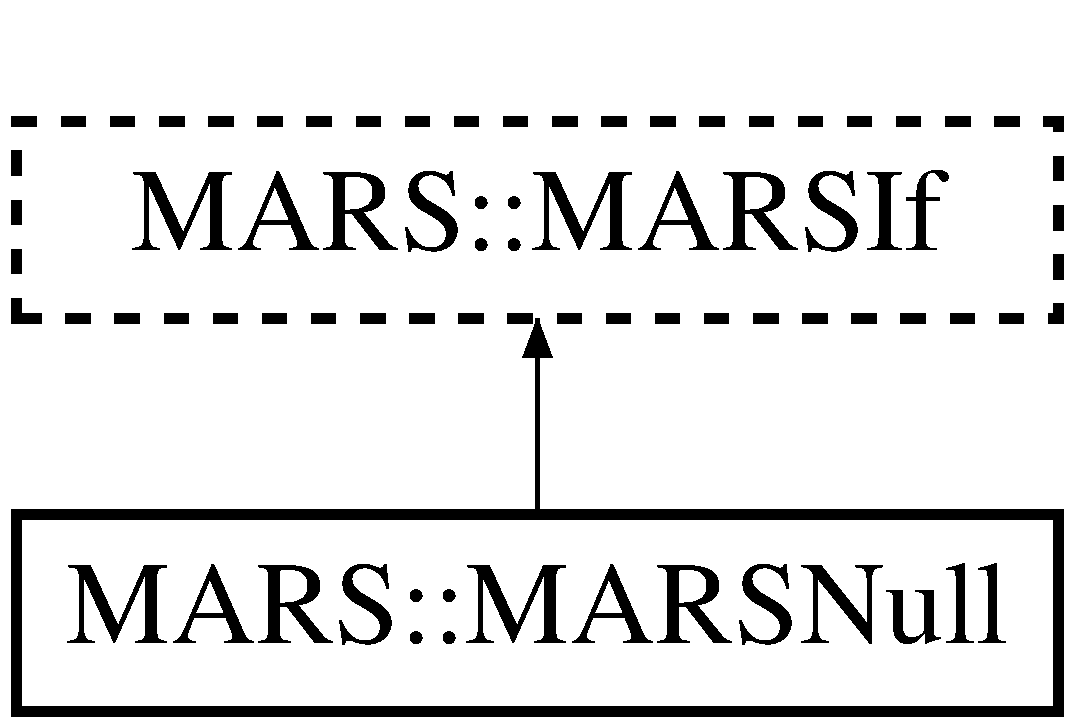
\includegraphics[height=2.000000cm]{classMARS_1_1MARSNull}
\end{center}
\end{figure}
\subsection*{Public Member Functions}
\begin{DoxyCompactItemize}
\item 
\mbox{\Hypertarget{classMARS_1_1MARSNull_a757644eb0ec614640b91ae07acb6e03c}\label{classMARS_1_1MARSNull_a757644eb0ec614640b91ae07acb6e03c}} 
void {\bfseries get\+Code} (std\+::string \&)
\item 
\mbox{\Hypertarget{classMARS_1_1MARSNull_a6def929cab98e11050cfb18ddfe5c931}\label{classMARS_1_1MARSNull_a6def929cab98e11050cfb18ddfe5c931}} 
void {\bfseries send\+Message} (std\+::string \&)
\item 
\mbox{\Hypertarget{classMARS_1_1MARSNull_ad190c9cacc0f2267e4e76400f2d4e150}\label{classMARS_1_1MARSNull_ad190c9cacc0f2267e4e76400f2d4e150}} 
void {\bfseries get\+Message} (const std\+::string \&)
\item 
\mbox{\Hypertarget{classMARS_1_1MARSNull_a55c02ba9310b54697619632fa6d5ce7e}\label{classMARS_1_1MARSNull_a55c02ba9310b54697619632fa6d5ce7e}} 
void {\bfseries receive\+From\+JS} (const \hyperlink{classMARS_1_1Code}{Code} \&)
\item 
\mbox{\Hypertarget{classMARS_1_1MARSNull_a313820c47569b0e7ae1c25893c663736}\label{classMARS_1_1MARSNull_a313820c47569b0e7ae1c25893c663736}} 
void {\bfseries get\+Color\+Table} (std\+::vector$<$ std\+::string $>$ \&)
\item 
\mbox{\Hypertarget{classMARS_1_1MARSNull_a35161e7232caef70ec72471e62c6861d}\label{classMARS_1_1MARSNull_a35161e7232caef70ec72471e62c6861d}} 
void {\bfseries set\+Color\+Table} (const std\+::vector$<$ std\+::string $>$ \&)
\end{DoxyCompactItemize}


The documentation for this class was generated from the following file\+:\begin{DoxyCompactItemize}
\item 
gen-\/cpp/M\+A\+R\+S.\+h\end{DoxyCompactItemize}

\hypertarget{classMarsOperation}{}\section{Mars\+Operation Class Reference}
\label{classMarsOperation}\index{Mars\+Operation@{Mars\+Operation}}


{\ttfamily \#include $<$Mars\+Operation.\+h$>$}

Inheritance diagram for Mars\+Operation\+:\begin{figure}[H]
\begin{center}
\leavevmode
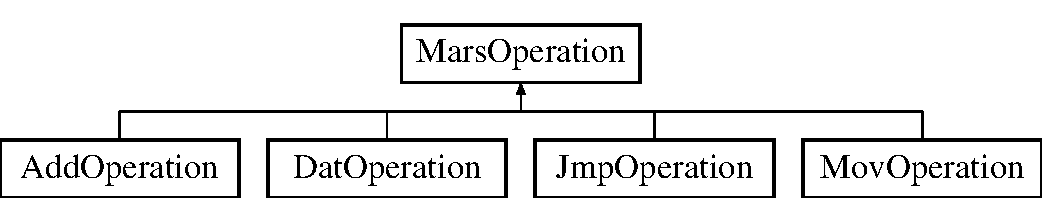
\includegraphics[height=2.000000cm]{classMarsOperation}
\end{center}
\end{figure}
\subsection*{Public Member Functions}
\begin{DoxyCompactItemize}
\item 
\mbox{\Hypertarget{classMarsOperation_ad9897bc8c38be46877392fd999444de7}\label{classMarsOperation_ad9897bc8c38be46877392fd999444de7}} 
{\bfseries Mars\+Operation} (const std\+::string op\+Code)
\item 
\mbox{\Hypertarget{classMarsOperation_a81cea2fbb13b712743fb53edfdff1962}\label{classMarsOperation_a81cea2fbb13b712743fb53edfdff1962}} 
const std\+::string \& {\bfseries get\+Op\+Code} () const
\item 
\mbox{\Hypertarget{classMarsOperation_ac152b465684f88621ce38f01d60cab49}\label{classMarsOperation_ac152b465684f88621ce38f01d60cab49}} 
virtual std\+::shared\+\_\+ptr$<$ \hyperlink{classProcessAction}{Process\+Action} $>$ {\bfseries run\+Operation} (\hyperlink{classOperationParamsMixed}{Operation\+Params\+Mixed} $\ast$oper\+Params)=0
\item 
\mbox{\Hypertarget{classMarsOperation_a38f03421e2eaf1c38514c97a893bed27}\label{classMarsOperation_a38f03421e2eaf1c38514c97a893bed27}} 
virtual std\+::shared\+\_\+ptr$<$ \hyperlink{classProcessAction}{Process\+Action} $>$ {\bfseries run\+Operation} (\hyperlink{classOperationParamsInstructions}{Operation\+Params\+Instructions} $\ast$oper\+Params)=0
\end{DoxyCompactItemize}


\subsection{Detailed Description}
Base class representing Operation 

The documentation for this class was generated from the following files\+:\begin{DoxyCompactItemize}
\item 
logic/mars/Mars\+Operation.\+h\item 
logic/mars/Mars\+Operation.\+cpp\end{DoxyCompactItemize}

\hypertarget{classMARS_1_1MARSProcessor}{}\section{M\+A\+RS\+:\+:M\+A\+R\+S\+Processor Class Reference}
\label{classMARS_1_1MARSProcessor}\index{M\+A\+R\+S\+::\+M\+A\+R\+S\+Processor@{M\+A\+R\+S\+::\+M\+A\+R\+S\+Processor}}
Inheritance diagram for M\+A\+RS\+:\+:M\+A\+R\+S\+Processor\+:\begin{figure}[H]
\begin{center}
\leavevmode
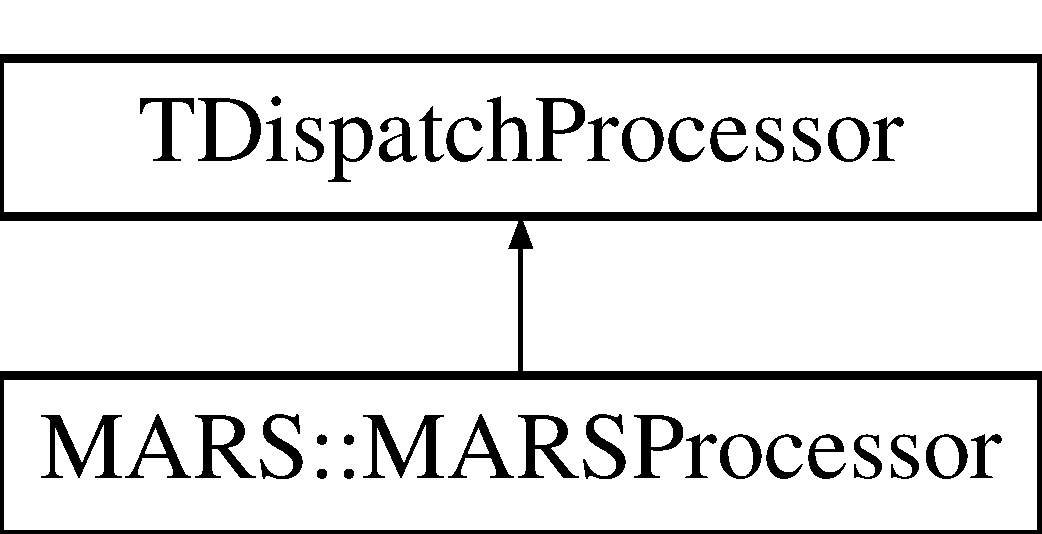
\includegraphics[height=2.000000cm]{classMARS_1_1MARSProcessor}
\end{center}
\end{figure}
\subsection*{Public Member Functions}
\begin{DoxyCompactItemize}
\item 
\mbox{\Hypertarget{classMARS_1_1MARSProcessor_a13e3d6f25435c7255b9f3d824aca8ab7}\label{classMARS_1_1MARSProcessor_a13e3d6f25435c7255b9f3d824aca8ab7}} 
{\bfseries M\+A\+R\+S\+Processor} (boost\+::shared\+\_\+ptr$<$ \hyperlink{classMARS_1_1MARSIf}{M\+A\+R\+S\+If} $>$ iface)
\end{DoxyCompactItemize}
\subsection*{Protected Member Functions}
\begin{DoxyCompactItemize}
\item 
\mbox{\Hypertarget{classMARS_1_1MARSProcessor_aa64fae822585f4dc16daf9175b69b60d}\label{classMARS_1_1MARSProcessor_aa64fae822585f4dc16daf9175b69b60d}} 
virtual bool {\bfseries dispatch\+Call} (\+::apache\+::thrift\+::protocol\+::\+T\+Protocol $\ast$iprot, \+::apache\+::thrift\+::protocol\+::\+T\+Protocol $\ast$oprot, const std\+::string \&fname, int32\+\_\+t seqid, void $\ast$call\+Context)
\end{DoxyCompactItemize}
\subsection*{Protected Attributes}
\begin{DoxyCompactItemize}
\item 
\mbox{\Hypertarget{classMARS_1_1MARSProcessor_a14cd99f66089463d642206898afbf266}\label{classMARS_1_1MARSProcessor_a14cd99f66089463d642206898afbf266}} 
boost\+::shared\+\_\+ptr$<$ \hyperlink{classMARS_1_1MARSIf}{M\+A\+R\+S\+If} $>$ {\bfseries iface\+\_\+}
\end{DoxyCompactItemize}


The documentation for this class was generated from the following files\+:\begin{DoxyCompactItemize}
\item 
gen-\/cpp/M\+A\+R\+S.\+h\item 
gen-\/cpp/M\+A\+R\+S.\+cpp\end{DoxyCompactItemize}

\hypertarget{classMARS_1_1MARSProcessorFactory}{}\section{M\+A\+RS\+:\+:M\+A\+R\+S\+Processor\+Factory Class Reference}
\label{classMARS_1_1MARSProcessorFactory}\index{M\+A\+R\+S\+::\+M\+A\+R\+S\+Processor\+Factory@{M\+A\+R\+S\+::\+M\+A\+R\+S\+Processor\+Factory}}
Inheritance diagram for M\+A\+RS\+:\+:M\+A\+R\+S\+Processor\+Factory\+:\begin{figure}[H]
\begin{center}
\leavevmode
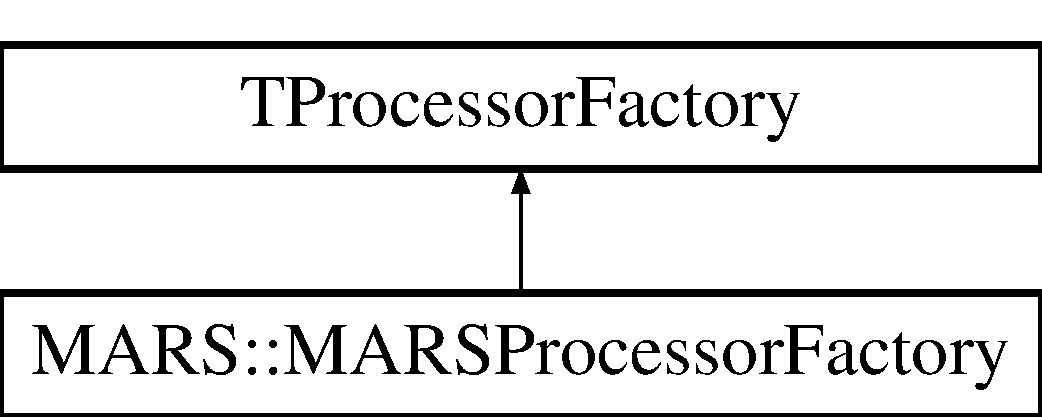
\includegraphics[height=2.000000cm]{classMARS_1_1MARSProcessorFactory}
\end{center}
\end{figure}
\subsection*{Public Member Functions}
\begin{DoxyCompactItemize}
\item 
\mbox{\Hypertarget{classMARS_1_1MARSProcessorFactory_a5995e5f3bde4390ed8dac9cf178aef36}\label{classMARS_1_1MARSProcessorFactory_a5995e5f3bde4390ed8dac9cf178aef36}} 
{\bfseries M\+A\+R\+S\+Processor\+Factory} (const \+::boost\+::shared\+\_\+ptr$<$ \hyperlink{classMARS_1_1MARSIfFactory}{M\+A\+R\+S\+If\+Factory} $>$ \&handler\+Factory)
\item 
\mbox{\Hypertarget{classMARS_1_1MARSProcessorFactory_a09dcb130d6c3b77b66c5a9245307ad7f}\label{classMARS_1_1MARSProcessorFactory_a09dcb130d6c3b77b66c5a9245307ad7f}} 
\+::boost\+::shared\+\_\+ptr$<$ \+::apache\+::thrift\+::\+T\+Processor $>$ {\bfseries get\+Processor} (const \+::apache\+::thrift\+::\+T\+Connection\+Info \&conn\+Info)
\end{DoxyCompactItemize}
\subsection*{Protected Attributes}
\begin{DoxyCompactItemize}
\item 
\mbox{\Hypertarget{classMARS_1_1MARSProcessorFactory_a352698490206c21fd31606a0f7ff8fb9}\label{classMARS_1_1MARSProcessorFactory_a352698490206c21fd31606a0f7ff8fb9}} 
\+::boost\+::shared\+\_\+ptr$<$ \hyperlink{classMARS_1_1MARSIfFactory}{M\+A\+R\+S\+If\+Factory} $>$ {\bfseries handler\+Factory\+\_\+}
\end{DoxyCompactItemize}


The documentation for this class was generated from the following files\+:\begin{DoxyCompactItemize}
\item 
gen-\/cpp/M\+A\+R\+S.\+h\item 
gen-\/cpp/M\+A\+R\+S.\+cpp\end{DoxyCompactItemize}

\hypertarget{classMarsResult}{}\section{Mars\+Result Class Reference}
\label{classMarsResult}\index{Mars\+Result@{Mars\+Result}}


The documentation for this class was generated from the following file\+:\begin{DoxyCompactItemize}
\item 
logic/Mars\+Result.\+h\end{DoxyCompactItemize}

\hypertarget{classMarsSimulator}{}\section{Mars\+Simulator Class Reference}
\label{classMarsSimulator}\index{Mars\+Simulator@{Mars\+Simulator}}
\subsection*{Public Member Functions}
\begin{DoxyCompactItemize}
\item 
\mbox{\Hypertarget{classMarsSimulator_a0d98b56cf57951938dfa4717740a0f46}\label{classMarsSimulator_a0d98b56cf57951938dfa4717740a0f46}} 
void {\bfseries set\+Instructions} (std\+::vector$<$ \hyperlink{classInstruction}{Instruction} $>$ instructions)
\item 
\mbox{\Hypertarget{classMarsSimulator_ac6cb4d312eb69f228de36e72d8482232}\label{classMarsSimulator_ac6cb4d312eb69f228de36e72d8482232}} 
std\+::vector$<$ \hyperlink{classInstruction}{Instruction} $>$ {\bfseries do\+Stuff} ()
\end{DoxyCompactItemize}


The documentation for this class was generated from the following files\+:\begin{DoxyCompactItemize}
\item 
logic/mars/Mars\+Simulator.\+h\item 
logic/mars/Mars\+Simulator.\+cpp\end{DoxyCompactItemize}

\hypertarget{structCatch_1_1Matchers_1_1Impl_1_1MatchAllOf}{}\section{Catch\+:\+:Matchers\+:\+:Impl\+:\+:Match\+All\+Of$<$ ArgT $>$ Struct Template Reference}
\label{structCatch_1_1Matchers_1_1Impl_1_1MatchAllOf}\index{Catch\+::\+Matchers\+::\+Impl\+::\+Match\+All\+Of$<$ Arg\+T $>$@{Catch\+::\+Matchers\+::\+Impl\+::\+Match\+All\+Of$<$ Arg\+T $>$}}
Inheritance diagram for Catch\+:\+:Matchers\+:\+:Impl\+:\+:Match\+All\+Of$<$ ArgT $>$\+:\begin{figure}[H]
\begin{center}
\leavevmode
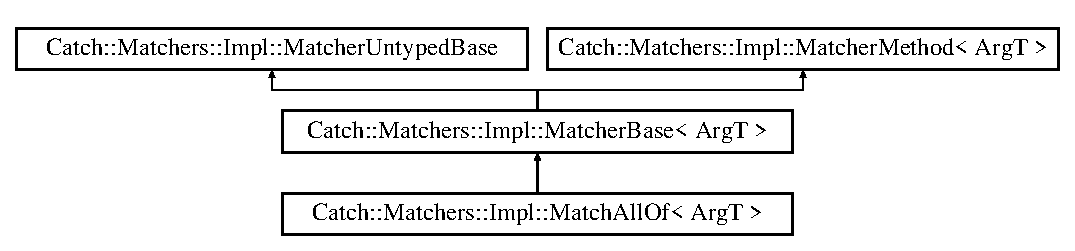
\includegraphics[height=2.926829cm]{structCatch_1_1Matchers_1_1Impl_1_1MatchAllOf}
\end{center}
\end{figure}
\subsection*{Public Member Functions}
\begin{DoxyCompactItemize}
\item 
\mbox{\Hypertarget{structCatch_1_1Matchers_1_1Impl_1_1MatchAllOf_a7bf0c2d8cedf67ecf9d0a527cb5a8263}\label{structCatch_1_1Matchers_1_1Impl_1_1MatchAllOf_a7bf0c2d8cedf67ecf9d0a527cb5a8263}} 
virtual bool {\bfseries match} (ArgT const \&arg) const C\+A\+T\+C\+H\+\_\+\+O\+V\+E\+R\+R\+I\+DE
\item 
\mbox{\Hypertarget{structCatch_1_1Matchers_1_1Impl_1_1MatchAllOf_aaefeba99a0b35425203468a65bff544b}\label{structCatch_1_1Matchers_1_1Impl_1_1MatchAllOf_aaefeba99a0b35425203468a65bff544b}} 
virtual std\+::string {\bfseries describe} () const C\+A\+T\+C\+H\+\_\+\+O\+V\+E\+R\+R\+I\+DE
\item 
\mbox{\Hypertarget{structCatch_1_1Matchers_1_1Impl_1_1MatchAllOf_a9d0e38b36474336498d627610db434f3}\label{structCatch_1_1Matchers_1_1Impl_1_1MatchAllOf_a9d0e38b36474336498d627610db434f3}} 
\hyperlink{structCatch_1_1Matchers_1_1Impl_1_1MatchAllOf}{Match\+All\+Of}$<$ ArgT $>$ \& {\bfseries operator\&\&} (\hyperlink{structCatch_1_1Matchers_1_1Impl_1_1MatcherBase}{Matcher\+Base}$<$ ArgT $>$ const \&other)
\end{DoxyCompactItemize}
\subsection*{Public Attributes}
\begin{DoxyCompactItemize}
\item 
\mbox{\Hypertarget{structCatch_1_1Matchers_1_1Impl_1_1MatchAllOf_a98d6a2611f195a4a5c49f92fd877be9a}\label{structCatch_1_1Matchers_1_1Impl_1_1MatchAllOf_a98d6a2611f195a4a5c49f92fd877be9a}} 
std\+::vector$<$ \hyperlink{structCatch_1_1Matchers_1_1Impl_1_1MatcherBase}{Matcher\+Base}$<$ ArgT $>$ const  $\ast$ $>$ {\bfseries m\+\_\+matchers}
\end{DoxyCompactItemize}
\subsection*{Additional Inherited Members}


The documentation for this struct was generated from the following file\+:\begin{DoxyCompactItemize}
\item 
test\+\_\+cases/catch.\+hpp\end{DoxyCompactItemize}

\hypertarget{structCatch_1_1Matchers_1_1Impl_1_1MatchAnyOf}{}\section{Catch\+:\+:Matchers\+:\+:Impl\+:\+:Match\+Any\+Of$<$ ArgT $>$ Struct Template Reference}
\label{structCatch_1_1Matchers_1_1Impl_1_1MatchAnyOf}\index{Catch\+::\+Matchers\+::\+Impl\+::\+Match\+Any\+Of$<$ Arg\+T $>$@{Catch\+::\+Matchers\+::\+Impl\+::\+Match\+Any\+Of$<$ Arg\+T $>$}}
Inheritance diagram for Catch\+:\+:Matchers\+:\+:Impl\+:\+:Match\+Any\+Of$<$ ArgT $>$\+:\begin{figure}[H]
\begin{center}
\leavevmode
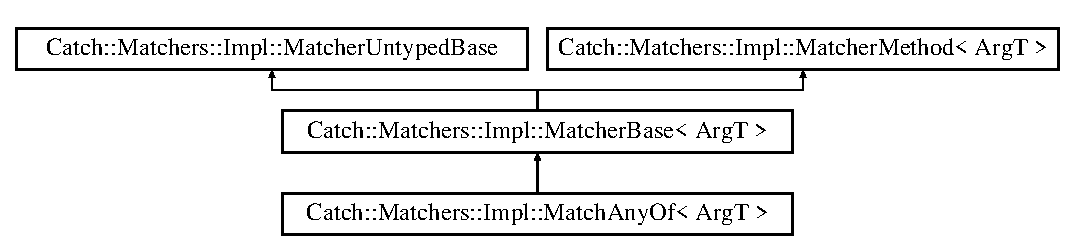
\includegraphics[height=2.926829cm]{structCatch_1_1Matchers_1_1Impl_1_1MatchAnyOf}
\end{center}
\end{figure}
\subsection*{Public Member Functions}
\begin{DoxyCompactItemize}
\item 
\mbox{\Hypertarget{structCatch_1_1Matchers_1_1Impl_1_1MatchAnyOf_a73be317ecf5919af855af96d68e714b9}\label{structCatch_1_1Matchers_1_1Impl_1_1MatchAnyOf_a73be317ecf5919af855af96d68e714b9}} 
virtual bool {\bfseries match} (ArgT const \&arg) const C\+A\+T\+C\+H\+\_\+\+O\+V\+E\+R\+R\+I\+DE
\item 
\mbox{\Hypertarget{structCatch_1_1Matchers_1_1Impl_1_1MatchAnyOf_a020f5d7889d8cd8be9ad309c690147b6}\label{structCatch_1_1Matchers_1_1Impl_1_1MatchAnyOf_a020f5d7889d8cd8be9ad309c690147b6}} 
virtual std\+::string {\bfseries describe} () const C\+A\+T\+C\+H\+\_\+\+O\+V\+E\+R\+R\+I\+DE
\item 
\mbox{\Hypertarget{structCatch_1_1Matchers_1_1Impl_1_1MatchAnyOf_a44d7582dbe09fc31b9a5ba8a6367b506}\label{structCatch_1_1Matchers_1_1Impl_1_1MatchAnyOf_a44d7582dbe09fc31b9a5ba8a6367b506}} 
\hyperlink{structCatch_1_1Matchers_1_1Impl_1_1MatchAnyOf}{Match\+Any\+Of}$<$ ArgT $>$ \& {\bfseries operator$\vert$$\vert$} (\hyperlink{structCatch_1_1Matchers_1_1Impl_1_1MatcherBase}{Matcher\+Base}$<$ ArgT $>$ const \&other)
\end{DoxyCompactItemize}
\subsection*{Public Attributes}
\begin{DoxyCompactItemize}
\item 
\mbox{\Hypertarget{structCatch_1_1Matchers_1_1Impl_1_1MatchAnyOf_a1fb1119e6110dc15b8d5262ec0aeddd5}\label{structCatch_1_1Matchers_1_1Impl_1_1MatchAnyOf_a1fb1119e6110dc15b8d5262ec0aeddd5}} 
std\+::vector$<$ \hyperlink{structCatch_1_1Matchers_1_1Impl_1_1MatcherBase}{Matcher\+Base}$<$ ArgT $>$ const  $\ast$ $>$ {\bfseries m\+\_\+matchers}
\end{DoxyCompactItemize}
\subsection*{Additional Inherited Members}


The documentation for this struct was generated from the following file\+:\begin{DoxyCompactItemize}
\item 
test\+\_\+cases/catch.\+hpp\end{DoxyCompactItemize}

\hypertarget{structCatch_1_1Matchers_1_1Impl_1_1MatcherBase}{}\section{Catch\+:\+:Matchers\+:\+:Impl\+:\+:Matcher\+Base$<$ ObjectT, ComparatorT $>$ Struct Template Reference}
\label{structCatch_1_1Matchers_1_1Impl_1_1MatcherBase}\index{Catch\+::\+Matchers\+::\+Impl\+::\+Matcher\+Base$<$ Object\+T, Comparator\+T $>$@{Catch\+::\+Matchers\+::\+Impl\+::\+Matcher\+Base$<$ Object\+T, Comparator\+T $>$}}
Inheritance diagram for Catch\+:\+:Matchers\+:\+:Impl\+:\+:Matcher\+Base$<$ ObjectT, ComparatorT $>$\+:\begin{figure}[H]
\begin{center}
\leavevmode
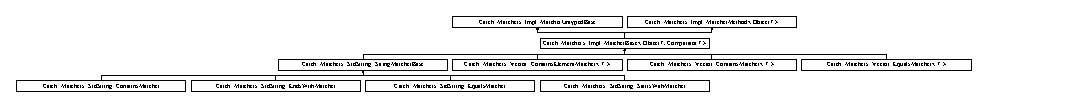
\includegraphics[height=1.006289cm]{structCatch_1_1Matchers_1_1Impl_1_1MatcherBase}
\end{center}
\end{figure}
\subsection*{Public Member Functions}
\begin{DoxyCompactItemize}
\item 
\mbox{\Hypertarget{structCatch_1_1Matchers_1_1Impl_1_1MatcherBase_a3deede6b29d20c15cb5efc79df40a520}\label{structCatch_1_1Matchers_1_1Impl_1_1MatcherBase_a3deede6b29d20c15cb5efc79df40a520}} 
\hyperlink{structCatch_1_1Matchers_1_1Impl_1_1MatchAllOf}{Match\+All\+Of}$<$ ComparatorT $>$ {\bfseries operator\&\&} (\hyperlink{structCatch_1_1Matchers_1_1Impl_1_1MatcherBase}{Matcher\+Base} const \&other) const
\item 
\mbox{\Hypertarget{structCatch_1_1Matchers_1_1Impl_1_1MatcherBase_ae0345ee76d109ac6d0241be261450ebc}\label{structCatch_1_1Matchers_1_1Impl_1_1MatcherBase_ae0345ee76d109ac6d0241be261450ebc}} 
\hyperlink{structCatch_1_1Matchers_1_1Impl_1_1MatchAnyOf}{Match\+Any\+Of}$<$ ComparatorT $>$ {\bfseries operator$\vert$$\vert$} (\hyperlink{structCatch_1_1Matchers_1_1Impl_1_1MatcherBase}{Matcher\+Base} const \&other) const
\item 
\mbox{\Hypertarget{structCatch_1_1Matchers_1_1Impl_1_1MatcherBase_a85174b5b27113f7bdc47c140c1c72602}\label{structCatch_1_1Matchers_1_1Impl_1_1MatcherBase_a85174b5b27113f7bdc47c140c1c72602}} 
\hyperlink{structCatch_1_1Matchers_1_1Impl_1_1MatchNotOf}{Match\+Not\+Of}$<$ ComparatorT $>$ {\bfseries operator!} () const
\end{DoxyCompactItemize}
\subsection*{Additional Inherited Members}


The documentation for this struct was generated from the following file\+:\begin{DoxyCompactItemize}
\item 
test\+\_\+cases/catch.\+hpp\end{DoxyCompactItemize}

\hypertarget{structCatch_1_1Matchers_1_1Impl_1_1MatcherMethod}{}\section{Catch\+:\+:Matchers\+:\+:Impl\+:\+:Matcher\+Method$<$ ObjectT $>$ Struct Template Reference}
\label{structCatch_1_1Matchers_1_1Impl_1_1MatcherMethod}\index{Catch\+::\+Matchers\+::\+Impl\+::\+Matcher\+Method$<$ Object\+T $>$@{Catch\+::\+Matchers\+::\+Impl\+::\+Matcher\+Method$<$ Object\+T $>$}}
Inheritance diagram for Catch\+:\+:Matchers\+:\+:Impl\+:\+:Matcher\+Method$<$ ObjectT $>$\+:\begin{figure}[H]
\begin{center}
\leavevmode
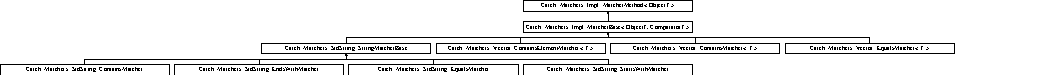
\includegraphics[height=1.006289cm]{structCatch_1_1Matchers_1_1Impl_1_1MatcherMethod}
\end{center}
\end{figure}
\subsection*{Public Member Functions}
\begin{DoxyCompactItemize}
\item 
\mbox{\Hypertarget{structCatch_1_1Matchers_1_1Impl_1_1MatcherMethod_ae0920ff9e817acf08e1bb0cbcb044e30}\label{structCatch_1_1Matchers_1_1Impl_1_1MatcherMethod_ae0920ff9e817acf08e1bb0cbcb044e30}} 
virtual bool {\bfseries match} (ObjectT const \&arg) const =0
\end{DoxyCompactItemize}


The documentation for this struct was generated from the following file\+:\begin{DoxyCompactItemize}
\item 
test\+\_\+cases/catch.\+hpp\end{DoxyCompactItemize}

\hypertarget{structCatch_1_1Matchers_1_1Impl_1_1MatcherMethod_3_01PtrT_01_5_01_4}{}\section{Catch\+:\+:Matchers\+:\+:Impl\+:\+:Matcher\+Method$<$ PtrT $\ast$ $>$ Struct Template Reference}
\label{structCatch_1_1Matchers_1_1Impl_1_1MatcherMethod_3_01PtrT_01_5_01_4}\index{Catch\+::\+Matchers\+::\+Impl\+::\+Matcher\+Method$<$ Ptr\+T $\ast$ $>$@{Catch\+::\+Matchers\+::\+Impl\+::\+Matcher\+Method$<$ Ptr\+T $\ast$ $>$}}
\subsection*{Public Member Functions}
\begin{DoxyCompactItemize}
\item 
\mbox{\Hypertarget{structCatch_1_1Matchers_1_1Impl_1_1MatcherMethod_3_01PtrT_01_5_01_4_a5fdd64f9509724f32ffc73cb320181d1}\label{structCatch_1_1Matchers_1_1Impl_1_1MatcherMethod_3_01PtrT_01_5_01_4_a5fdd64f9509724f32ffc73cb320181d1}} 
virtual bool {\bfseries match} (PtrT $\ast$arg) const =0
\end{DoxyCompactItemize}


The documentation for this struct was generated from the following file\+:\begin{DoxyCompactItemize}
\item 
test\+\_\+cases/catch.\+hpp\end{DoxyCompactItemize}

\hypertarget{classCatch_1_1Matchers_1_1Impl_1_1MatcherUntypedBase}{}\section{Catch\+:\+:Matchers\+:\+:Impl\+:\+:Matcher\+Untyped\+Base Class Reference}
\label{classCatch_1_1Matchers_1_1Impl_1_1MatcherUntypedBase}\index{Catch\+::\+Matchers\+::\+Impl\+::\+Matcher\+Untyped\+Base@{Catch\+::\+Matchers\+::\+Impl\+::\+Matcher\+Untyped\+Base}}
Inheritance diagram for Catch\+:\+:Matchers\+:\+:Impl\+:\+:Matcher\+Untyped\+Base\+:\begin{figure}[H]
\begin{center}
\leavevmode
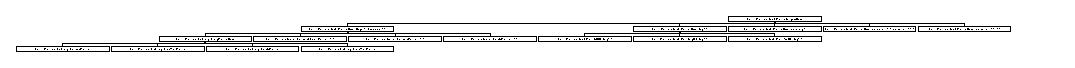
\includegraphics[height=0.471380cm]{classCatch_1_1Matchers_1_1Impl_1_1MatcherUntypedBase}
\end{center}
\end{figure}
\subsection*{Public Member Functions}
\begin{DoxyCompactItemize}
\item 
\mbox{\Hypertarget{classCatch_1_1Matchers_1_1Impl_1_1MatcherUntypedBase_a5982c7c80ca71dfe2298babadad7a453}\label{classCatch_1_1Matchers_1_1Impl_1_1MatcherUntypedBase_a5982c7c80ca71dfe2298babadad7a453}} 
std\+::string {\bfseries to\+String} () const
\end{DoxyCompactItemize}
\subsection*{Protected Member Functions}
\begin{DoxyCompactItemize}
\item 
\mbox{\Hypertarget{classCatch_1_1Matchers_1_1Impl_1_1MatcherUntypedBase_a91d3a907dbfcbb596077df24f6e11fe2}\label{classCatch_1_1Matchers_1_1Impl_1_1MatcherUntypedBase_a91d3a907dbfcbb596077df24f6e11fe2}} 
virtual std\+::string {\bfseries describe} () const =0
\end{DoxyCompactItemize}
\subsection*{Protected Attributes}
\begin{DoxyCompactItemize}
\item 
\mbox{\Hypertarget{classCatch_1_1Matchers_1_1Impl_1_1MatcherUntypedBase_a951095c462657e7097a9a6dc4dde813f}\label{classCatch_1_1Matchers_1_1Impl_1_1MatcherUntypedBase_a951095c462657e7097a9a6dc4dde813f}} 
std\+::string {\bfseries m\+\_\+cached\+To\+String}
\end{DoxyCompactItemize}


The documentation for this class was generated from the following file\+:\begin{DoxyCompactItemize}
\item 
test\+\_\+cases/catch.\+hpp\end{DoxyCompactItemize}

\hypertarget{classCatch_1_1MatchExpression}{}\section{Catch\+:\+:Match\+Expression$<$ ArgT, MatcherT $>$ Class Template Reference}
\label{classCatch_1_1MatchExpression}\index{Catch\+::\+Match\+Expression$<$ Arg\+T, Matcher\+T $>$@{Catch\+::\+Match\+Expression$<$ Arg\+T, Matcher\+T $>$}}
Inheritance diagram for Catch\+:\+:Match\+Expression$<$ ArgT, MatcherT $>$\+:\begin{figure}[H]
\begin{center}
\leavevmode
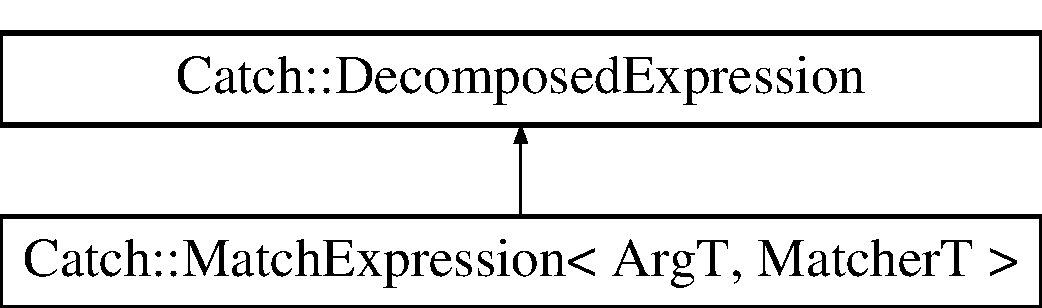
\includegraphics[height=2.000000cm]{classCatch_1_1MatchExpression}
\end{center}
\end{figure}
\subsection*{Public Member Functions}
\begin{DoxyCompactItemize}
\item 
\mbox{\Hypertarget{classCatch_1_1MatchExpression_a506f25bad7970cb35f9dbe54763a8ca5}\label{classCatch_1_1MatchExpression_a506f25bad7970cb35f9dbe54763a8ca5}} 
{\bfseries Match\+Expression} (ArgT arg, MatcherT matcher, char const $\ast$matcher\+String)
\item 
\mbox{\Hypertarget{classCatch_1_1MatchExpression_ac4edf6e9a6e5762a487db1486d0d1f45}\label{classCatch_1_1MatchExpression_ac4edf6e9a6e5762a487db1486d0d1f45}} 
virtual bool {\bfseries is\+Binary\+Expression} () const C\+A\+T\+C\+H\+\_\+\+O\+V\+E\+R\+R\+I\+DE
\item 
\mbox{\Hypertarget{classCatch_1_1MatchExpression_a4410a93bc5b8241eb2502f400fce7ec4}\label{classCatch_1_1MatchExpression_a4410a93bc5b8241eb2502f400fce7ec4}} 
virtual void {\bfseries reconstruct\+Expression} (std\+::string \&dest) const C\+A\+T\+C\+H\+\_\+\+O\+V\+E\+R\+R\+I\+DE
\end{DoxyCompactItemize}


The documentation for this class was generated from the following file\+:\begin{DoxyCompactItemize}
\item 
test\+\_\+cases/catch.\+hpp\end{DoxyCompactItemize}

\hypertarget{structCatch_1_1Matchers_1_1Impl_1_1MatchNotOf}{}\section{Catch\+:\+:Matchers\+:\+:Impl\+:\+:Match\+Not\+Of$<$ ArgT $>$ Struct Template Reference}
\label{structCatch_1_1Matchers_1_1Impl_1_1MatchNotOf}\index{Catch\+::\+Matchers\+::\+Impl\+::\+Match\+Not\+Of$<$ Arg\+T $>$@{Catch\+::\+Matchers\+::\+Impl\+::\+Match\+Not\+Of$<$ Arg\+T $>$}}
Inheritance diagram for Catch\+:\+:Matchers\+:\+:Impl\+:\+:Match\+Not\+Of$<$ ArgT $>$\+:\begin{figure}[H]
\begin{center}
\leavevmode
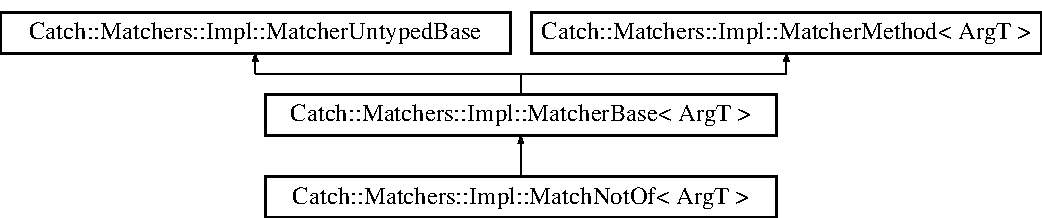
\includegraphics[height=2.926829cm]{structCatch_1_1Matchers_1_1Impl_1_1MatchNotOf}
\end{center}
\end{figure}
\subsection*{Public Member Functions}
\begin{DoxyCompactItemize}
\item 
\mbox{\Hypertarget{structCatch_1_1Matchers_1_1Impl_1_1MatchNotOf_a47afdd9e4c3354cef85adc3186097ae4}\label{structCatch_1_1Matchers_1_1Impl_1_1MatchNotOf_a47afdd9e4c3354cef85adc3186097ae4}} 
{\bfseries Match\+Not\+Of} (\hyperlink{structCatch_1_1Matchers_1_1Impl_1_1MatcherBase}{Matcher\+Base}$<$ ArgT $>$ const \&underlying\+Matcher)
\item 
\mbox{\Hypertarget{structCatch_1_1Matchers_1_1Impl_1_1MatchNotOf_a1b9ad6566e4ab0f292d2903f557307cc}\label{structCatch_1_1Matchers_1_1Impl_1_1MatchNotOf_a1b9ad6566e4ab0f292d2903f557307cc}} 
virtual bool {\bfseries match} (ArgT const \&arg) const C\+A\+T\+C\+H\+\_\+\+O\+V\+E\+R\+R\+I\+DE
\item 
\mbox{\Hypertarget{structCatch_1_1Matchers_1_1Impl_1_1MatchNotOf_a62bdc7dcb9ff000438a4ed3d5483a248}\label{structCatch_1_1Matchers_1_1Impl_1_1MatchNotOf_a62bdc7dcb9ff000438a4ed3d5483a248}} 
virtual std\+::string {\bfseries describe} () const C\+A\+T\+C\+H\+\_\+\+O\+V\+E\+R\+R\+I\+DE
\end{DoxyCompactItemize}
\subsection*{Public Attributes}
\begin{DoxyCompactItemize}
\item 
\mbox{\Hypertarget{structCatch_1_1Matchers_1_1Impl_1_1MatchNotOf_af7ac67f112b0e93796b048a47329aad4}\label{structCatch_1_1Matchers_1_1Impl_1_1MatchNotOf_af7ac67f112b0e93796b048a47329aad4}} 
\hyperlink{structCatch_1_1Matchers_1_1Impl_1_1MatcherBase}{Matcher\+Base}$<$ ArgT $>$ const  \& {\bfseries m\+\_\+underlying\+Matcher}
\end{DoxyCompactItemize}
\subsection*{Additional Inherited Members}


The documentation for this struct was generated from the following file\+:\begin{DoxyCompactItemize}
\item 
test\+\_\+cases/catch.\+hpp\end{DoxyCompactItemize}

\hypertarget{classMemoryIndex}{}\section{Memory\+Index Class Reference}
\label{classMemoryIndex}\index{Memory\+Index@{Memory\+Index}}
\subsection*{Public Member Functions}
\begin{DoxyCompactItemize}
\item 
\mbox{\Hypertarget{classMemoryIndex_a8ba4d0ed483633f22f394afc75bbd363}\label{classMemoryIndex_a8ba4d0ed483633f22f394afc75bbd363}} 
{\bfseries Memory\+Index} (int index)
\item 
\mbox{\Hypertarget{classMemoryIndex_a099a6efe3d15752206db4e0a6cfde758}\label{classMemoryIndex_a099a6efe3d15752206db4e0a6cfde758}} 
\hyperlink{classMemoryIndex}{Memory\+Index} \& {\bfseries operator++} ()
\item 
\mbox{\Hypertarget{classMemoryIndex_a1bfedace329ab61eea1e18c2dd6971a3}\label{classMemoryIndex_a1bfedace329ab61eea1e18c2dd6971a3}} 
\hyperlink{classMemoryIndex}{Memory\+Index} {\bfseries operator++} (int)
\item 
\mbox{\Hypertarget{classMemoryIndex_ad090f29c22ac178bbca8a00f57b6873e}\label{classMemoryIndex_ad090f29c22ac178bbca8a00f57b6873e}} 
int {\bfseries operator$\ast$} () const
\item 
\mbox{\Hypertarget{classMemoryIndex_ad9c7e20d9d1c5ed1a19cc3334d8a5872}\label{classMemoryIndex_ad9c7e20d9d1c5ed1a19cc3334d8a5872}} 
\hyperlink{classMemoryIndex}{Memory\+Index} {\bfseries operator+} (int)
\item 
\mbox{\Hypertarget{classMemoryIndex_a15bac8ea73954ee665e05c3f018d291f}\label{classMemoryIndex_a15bac8ea73954ee665e05c3f018d291f}} 
\hyperlink{classMemoryIndex}{Memory\+Index} \& {\bfseries operator+=} (int)
\item 
\mbox{\Hypertarget{classMemoryIndex_a5f9fe18cb9d41d5625fa1f4191bd9794}\label{classMemoryIndex_a5f9fe18cb9d41d5625fa1f4191bd9794}} 
\hyperlink{classMemoryIndex}{Memory\+Index} {\bfseries operator-\/} (int)
\item 
\mbox{\Hypertarget{classMemoryIndex_af5854bfbf3b1fc93b68291426de1dd14}\label{classMemoryIndex_af5854bfbf3b1fc93b68291426de1dd14}} 
\hyperlink{classMemoryIndex}{Memory\+Index} \& {\bfseries operator-\/=} (int)
\item 
\mbox{\Hypertarget{classMemoryIndex_af8cebaa913daaad29d4cbf1683456392}\label{classMemoryIndex_af8cebaa913daaad29d4cbf1683456392}} 
bool {\bfseries operator==} (int)
\end{DoxyCompactItemize}


The documentation for this class was generated from the following files\+:\begin{DoxyCompactItemize}
\item 
logic/mars/Memory\+Index.\+h\item 
logic/mars/Memory\+Index.\+cpp\end{DoxyCompactItemize}

\hypertarget{structCatch_1_1MessageBuilder}{}\section{Catch\+:\+:Message\+Builder Struct Reference}
\label{structCatch_1_1MessageBuilder}\index{Catch\+::\+Message\+Builder@{Catch\+::\+Message\+Builder}}
\subsection*{Public Member Functions}
\begin{DoxyCompactItemize}
\item 
\mbox{\Hypertarget{structCatch_1_1MessageBuilder_ab0c6378e722680bf58852c6ee2b6e724}\label{structCatch_1_1MessageBuilder_ab0c6378e722680bf58852c6ee2b6e724}} 
{\bfseries Message\+Builder} (std\+::string const \&macro\+Name, \hyperlink{structCatch_1_1SourceLineInfo}{Source\+Line\+Info} const \&line\+Info, Result\+Was\+::\+Of\+Type type)
\item 
\mbox{\Hypertarget{structCatch_1_1MessageBuilder_a20fa48d069b20dddcc2d3df8abb123c1}\label{structCatch_1_1MessageBuilder_a20fa48d069b20dddcc2d3df8abb123c1}} 
{\footnotesize template$<$typename T $>$ }\\\hyperlink{structCatch_1_1MessageBuilder}{Message\+Builder} \& {\bfseries operator$<$$<$} (T const \&value)
\end{DoxyCompactItemize}
\subsection*{Public Attributes}
\begin{DoxyCompactItemize}
\item 
\mbox{\Hypertarget{structCatch_1_1MessageBuilder_a979f1c2b36d78f80ee275bfa5ba0209f}\label{structCatch_1_1MessageBuilder_a979f1c2b36d78f80ee275bfa5ba0209f}} 
\hyperlink{structCatch_1_1MessageInfo}{Message\+Info} {\bfseries m\+\_\+info}
\item 
\mbox{\Hypertarget{structCatch_1_1MessageBuilder_a6488ab0cc4ea52affc9c0612c7c5df6b}\label{structCatch_1_1MessageBuilder_a6488ab0cc4ea52affc9c0612c7c5df6b}} 
std\+::ostringstream {\bfseries m\+\_\+stream}
\end{DoxyCompactItemize}


The documentation for this struct was generated from the following file\+:\begin{DoxyCompactItemize}
\item 
test\+\_\+cases/catch.\+hpp\end{DoxyCompactItemize}

\hypertarget{structCatch_1_1MessageInfo}{}\section{Catch\+:\+:Message\+Info Struct Reference}
\label{structCatch_1_1MessageInfo}\index{Catch\+::\+Message\+Info@{Catch\+::\+Message\+Info}}
\subsection*{Public Member Functions}
\begin{DoxyCompactItemize}
\item 
\mbox{\Hypertarget{structCatch_1_1MessageInfo_a2e336c33ebef7af3c1bbae6a56e14f8a}\label{structCatch_1_1MessageInfo_a2e336c33ebef7af3c1bbae6a56e14f8a}} 
{\bfseries Message\+Info} (std\+::string const \&\+\_\+macro\+Name, \hyperlink{structCatch_1_1SourceLineInfo}{Source\+Line\+Info} const \&\+\_\+line\+Info, Result\+Was\+::\+Of\+Type \+\_\+type)
\item 
\mbox{\Hypertarget{structCatch_1_1MessageInfo_af4b37f2172ba55395813b4bb6bbbde1a}\label{structCatch_1_1MessageInfo_af4b37f2172ba55395813b4bb6bbbde1a}} 
bool {\bfseries operator==} (\hyperlink{structCatch_1_1MessageInfo}{Message\+Info} const \&other) const
\item 
\mbox{\Hypertarget{structCatch_1_1MessageInfo_a8254cb8fca2da02a29a9843cdcb79df1}\label{structCatch_1_1MessageInfo_a8254cb8fca2da02a29a9843cdcb79df1}} 
bool {\bfseries operator$<$} (\hyperlink{structCatch_1_1MessageInfo}{Message\+Info} const \&other) const
\end{DoxyCompactItemize}
\subsection*{Public Attributes}
\begin{DoxyCompactItemize}
\item 
\mbox{\Hypertarget{structCatch_1_1MessageInfo_a156ade4b3cc731f6ec7b542ae47ba8e3}\label{structCatch_1_1MessageInfo_a156ade4b3cc731f6ec7b542ae47ba8e3}} 
std\+::string {\bfseries macro\+Name}
\item 
\mbox{\Hypertarget{structCatch_1_1MessageInfo_a985165328723e599696ebd8e43195cc5}\label{structCatch_1_1MessageInfo_a985165328723e599696ebd8e43195cc5}} 
\hyperlink{structCatch_1_1SourceLineInfo}{Source\+Line\+Info} {\bfseries line\+Info}
\item 
\mbox{\Hypertarget{structCatch_1_1MessageInfo_ae928b9117465c696e45951d9d0284e78}\label{structCatch_1_1MessageInfo_ae928b9117465c696e45951d9d0284e78}} 
Result\+Was\+::\+Of\+Type {\bfseries type}
\item 
\mbox{\Hypertarget{structCatch_1_1MessageInfo_ab6cd06e050bf426c6577502a5c50e256}\label{structCatch_1_1MessageInfo_ab6cd06e050bf426c6577502a5c50e256}} 
std\+::string {\bfseries message}
\item 
\mbox{\Hypertarget{structCatch_1_1MessageInfo_a7f4f57ea21e50160adefce7b68a781d6}\label{structCatch_1_1MessageInfo_a7f4f57ea21e50160adefce7b68a781d6}} 
unsigned int {\bfseries sequence}
\end{DoxyCompactItemize}


The documentation for this struct was generated from the following file\+:\begin{DoxyCompactItemize}
\item 
test\+\_\+cases/catch.\+hpp\end{DoxyCompactItemize}

\hypertarget{classCatch_1_1MethodTestCase}{}\section{Catch\+:\+:Method\+Test\+Case$<$ C $>$ Class Template Reference}
\label{classCatch_1_1MethodTestCase}\index{Catch\+::\+Method\+Test\+Case$<$ C $>$@{Catch\+::\+Method\+Test\+Case$<$ C $>$}}
Inheritance diagram for Catch\+:\+:Method\+Test\+Case$<$ C $>$\+:\begin{figure}[H]
\begin{center}
\leavevmode
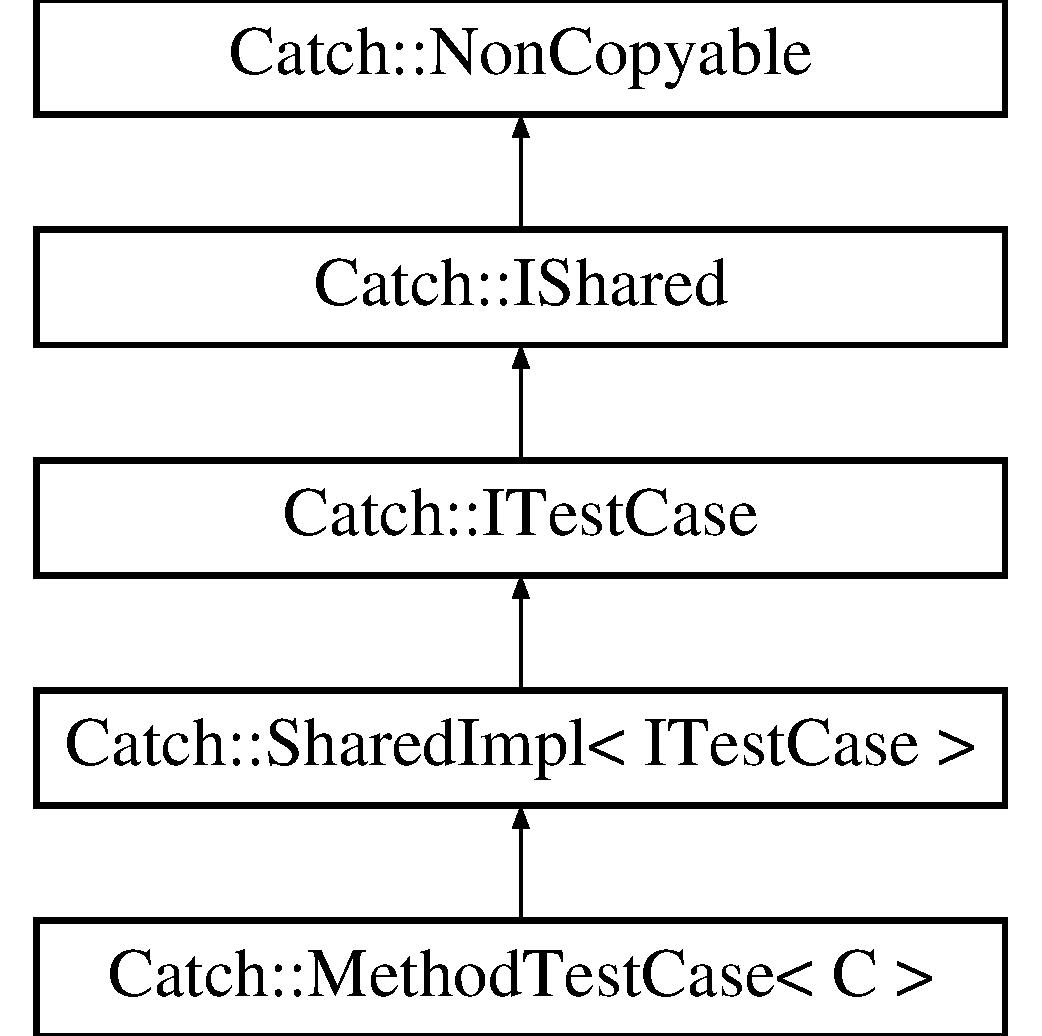
\includegraphics[height=5.000000cm]{classCatch_1_1MethodTestCase}
\end{center}
\end{figure}
\subsection*{Public Member Functions}
\begin{DoxyCompactItemize}
\item 
\mbox{\Hypertarget{classCatch_1_1MethodTestCase_a7b043b85dae371358255dd9dc6582e7b}\label{classCatch_1_1MethodTestCase_a7b043b85dae371358255dd9dc6582e7b}} 
{\bfseries Method\+Test\+Case} (void(C\+::$\ast$method)())
\item 
\mbox{\Hypertarget{classCatch_1_1MethodTestCase_a4e2263cfa0646f2980768328cb372793}\label{classCatch_1_1MethodTestCase_a4e2263cfa0646f2980768328cb372793}} 
virtual void {\bfseries invoke} () const
\end{DoxyCompactItemize}
\subsection*{Additional Inherited Members}


The documentation for this class was generated from the following file\+:\begin{DoxyCompactItemize}
\item 
test\+\_\+cases/catch.\+hpp\end{DoxyCompactItemize}

\hypertarget{classModifierFactory}{}\section{Modifier\+Factory Class Reference}
\label{classModifierFactory}\index{Modifier\+Factory@{Modifier\+Factory}}


{\ttfamily \#include $<$Modifier\+Factory.\+h$>$}

\subsection*{Static Public Member Functions}
\begin{DoxyCompactItemize}
\item 
static std\+::shared\+\_\+ptr$<$ \hyperlink{classInstructionModifier}{Instruction\+Modifier} $>$ \hyperlink{classModifierFactory_a2c5bcf63ebfe5acd617783ffb6468ec7}{create\+Modifier} (const char raw\+Modifier)
\item 
static bool \hyperlink{classModifierFactory_a44341cfff086fc453d24fe5d01c8bfa6}{is\+Modifier\+Omitted} (const char modifier)
\item 
static std\+::shared\+\_\+ptr$<$ \hyperlink{classInstructionModifier}{Instruction\+Modifier} $>$ \hyperlink{classModifierFactory_af215ef0d0aa2e9e4860148fecfe952f8}{create\+Default\+Modifier} ()
\end{DoxyCompactItemize}


\subsection{Detailed Description}
Class managing creating instruction modifiers, implementing factory design pattern 

\subsection{Member Function Documentation}
\mbox{\Hypertarget{classModifierFactory_af215ef0d0aa2e9e4860148fecfe952f8}\label{classModifierFactory_af215ef0d0aa2e9e4860148fecfe952f8}} 
\index{Modifier\+Factory@{Modifier\+Factory}!create\+Default\+Modifier@{create\+Default\+Modifier}}
\index{create\+Default\+Modifier@{create\+Default\+Modifier}!Modifier\+Factory@{Modifier\+Factory}}
\subsubsection{\texorpdfstring{create\+Default\+Modifier()}{createDefaultModifier()}}
{\footnotesize\ttfamily std\+::shared\+\_\+ptr$<$ \hyperlink{classInstructionModifier}{Instruction\+Modifier} $>$ Modifier\+Factory\+::create\+Default\+Modifier (\begin{DoxyParamCaption}{ }\end{DoxyParamCaption})\hspace{0.3cm}{\ttfamily [static]}}

Creates shared pointer to object initialized with default constructor \begin{DoxyReturn}{Returns}
pointer to \hyperlink{classDirectInstructionModifier}{Direct\+Instruction\+Modifier} 
\end{DoxyReturn}
\mbox{\Hypertarget{classModifierFactory_a2c5bcf63ebfe5acd617783ffb6468ec7}\label{classModifierFactory_a2c5bcf63ebfe5acd617783ffb6468ec7}} 
\index{Modifier\+Factory@{Modifier\+Factory}!create\+Modifier@{create\+Modifier}}
\index{create\+Modifier@{create\+Modifier}!Modifier\+Factory@{Modifier\+Factory}}
\subsubsection{\texorpdfstring{create\+Modifier()}{createModifier()}}
{\footnotesize\ttfamily std\+::shared\+\_\+ptr$<$ \hyperlink{classInstructionModifier}{Instruction\+Modifier} $>$ Modifier\+Factory\+::create\+Modifier (\begin{DoxyParamCaption}\item[{const char}]{raw\+Modifier }\end{DoxyParamCaption})\hspace{0.3cm}{\ttfamily [static]}}

Creates instruction modfiers 
\begin{DoxyParams}{Parameters}
{\em raw\+Modifier} & \hyperlink{classInstruction}{Instruction} modifier code \\
\hline
\end{DoxyParams}
\begin{DoxyReturn}{Returns}
\hyperlink{classInstructionModifier}{Instruction\+Modifier} object of class deduced from code 
\end{DoxyReturn}
\mbox{\Hypertarget{classModifierFactory_a44341cfff086fc453d24fe5d01c8bfa6}\label{classModifierFactory_a44341cfff086fc453d24fe5d01c8bfa6}} 
\index{Modifier\+Factory@{Modifier\+Factory}!is\+Modifier\+Omitted@{is\+Modifier\+Omitted}}
\index{is\+Modifier\+Omitted@{is\+Modifier\+Omitted}!Modifier\+Factory@{Modifier\+Factory}}
\subsubsection{\texorpdfstring{is\+Modifier\+Omitted()}{isModifierOmitted()}}
{\footnotesize\ttfamily bool Modifier\+Factory\+::is\+Modifier\+Omitted (\begin{DoxyParamCaption}\item[{const char}]{modifier }\end{DoxyParamCaption})\hspace{0.3cm}{\ttfamily [static]}}


\begin{DoxyParams}{Parameters}
{\em modifier} & \\
\hline
\end{DoxyParams}
\begin{DoxyReturn}{Returns}
true if modifier equals \char`\"{}-\/\char`\"{} or is digit 
\end{DoxyReturn}


The documentation for this class was generated from the following files\+:\begin{DoxyCompactItemize}
\item 
logic/parser/Modifier\+Factory.\+h\item 
logic/parser/Modifier\+Factory.\+cpp\end{DoxyCompactItemize}

\hypertarget{classMovOperation}{}\section{Mov\+Operation Class Reference}
\label{classMovOperation}\index{Mov\+Operation@{Mov\+Operation}}


{\ttfamily \#include $<$Mov\+Operation.\+h$>$}

Inheritance diagram for Mov\+Operation\+:\begin{figure}[H]
\begin{center}
\leavevmode
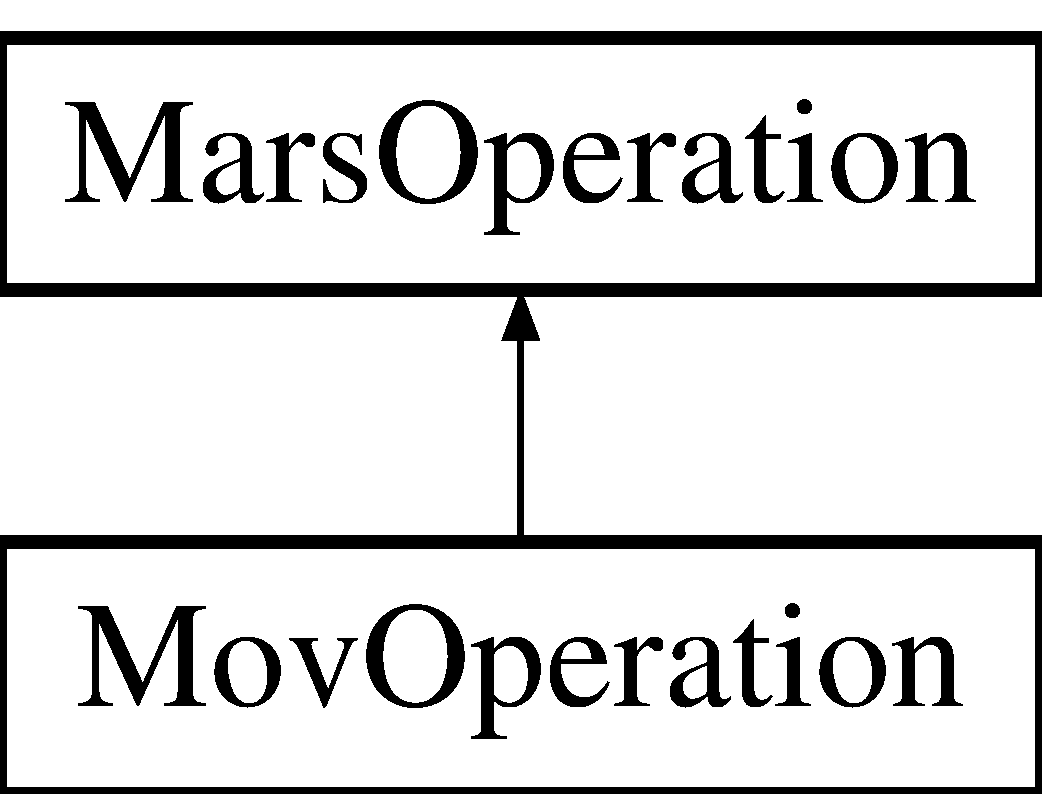
\includegraphics[height=2.000000cm]{classMovOperation}
\end{center}
\end{figure}
\subsection*{Public Member Functions}
\begin{DoxyCompactItemize}
\item 
\mbox{\Hypertarget{classMovOperation_a0d212f53fcc541ee5f934e19cca0ba46}\label{classMovOperation_a0d212f53fcc541ee5f934e19cca0ba46}} 
virtual std\+::shared\+\_\+ptr$<$ \hyperlink{classProcessAction}{Process\+Action} $>$ {\bfseries run\+Operation} (\hyperlink{classOperationParamsInstructions}{Operation\+Params\+Instructions} $\ast$oper\+Params) override
\item 
\mbox{\Hypertarget{classMovOperation_adb37649782b83a02cd24f54445297cba}\label{classMovOperation_adb37649782b83a02cd24f54445297cba}} 
virtual std\+::shared\+\_\+ptr$<$ \hyperlink{classProcessAction}{Process\+Action} $>$ {\bfseries run\+Operation} (\hyperlink{classOperationParamsMixed}{Operation\+Params\+Mixed} $\ast$oper\+Params) override
\end{DoxyCompactItemize}


\subsection{Detailed Description}
Class representing M\+OV operation 

The documentation for this class was generated from the following files\+:\begin{DoxyCompactItemize}
\item 
logic/mars/Mov\+Operation.\+h\item 
logic/mars/Mov\+Operation.\+cpp\end{DoxyCompactItemize}

\hypertarget{structCatch_1_1NameAndDesc}{}\section{Catch\+:\+:Name\+And\+Desc Struct Reference}
\label{structCatch_1_1NameAndDesc}\index{Catch\+::\+Name\+And\+Desc@{Catch\+::\+Name\+And\+Desc}}
\subsection*{Public Member Functions}
\begin{DoxyCompactItemize}
\item 
\mbox{\Hypertarget{structCatch_1_1NameAndDesc_a189ceb9942fb5f6635140d6a09fc843a}\label{structCatch_1_1NameAndDesc_a189ceb9942fb5f6635140d6a09fc843a}} 
{\bfseries Name\+And\+Desc} (const char $\ast$\+\_\+name=\char`\"{}\char`\"{}, const char $\ast$\+\_\+description=\char`\"{}\char`\"{})
\end{DoxyCompactItemize}
\subsection*{Public Attributes}
\begin{DoxyCompactItemize}
\item 
\mbox{\Hypertarget{structCatch_1_1NameAndDesc_a374b4ed8be3cf98be20ebde5273bde51}\label{structCatch_1_1NameAndDesc_a374b4ed8be3cf98be20ebde5273bde51}} 
const char $\ast$ {\bfseries name}
\item 
\mbox{\Hypertarget{structCatch_1_1NameAndDesc_a3463a23ff65ce494fc380452b57b7970}\label{structCatch_1_1NameAndDesc_a3463a23ff65ce494fc380452b57b7970}} 
const char $\ast$ {\bfseries description}
\end{DoxyCompactItemize}


The documentation for this struct was generated from the following file\+:\begin{DoxyCompactItemize}
\item 
test\+\_\+cases/catch.\+hpp\end{DoxyCompactItemize}

\hypertarget{classCatch_1_1NonCopyable}{}\section{Catch\+:\+:Non\+Copyable Class Reference}
\label{classCatch_1_1NonCopyable}\index{Catch\+::\+Non\+Copyable@{Catch\+::\+Non\+Copyable}}
Inheritance diagram for Catch\+:\+:Non\+Copyable\+:\begin{figure}[H]
\begin{center}
\leavevmode
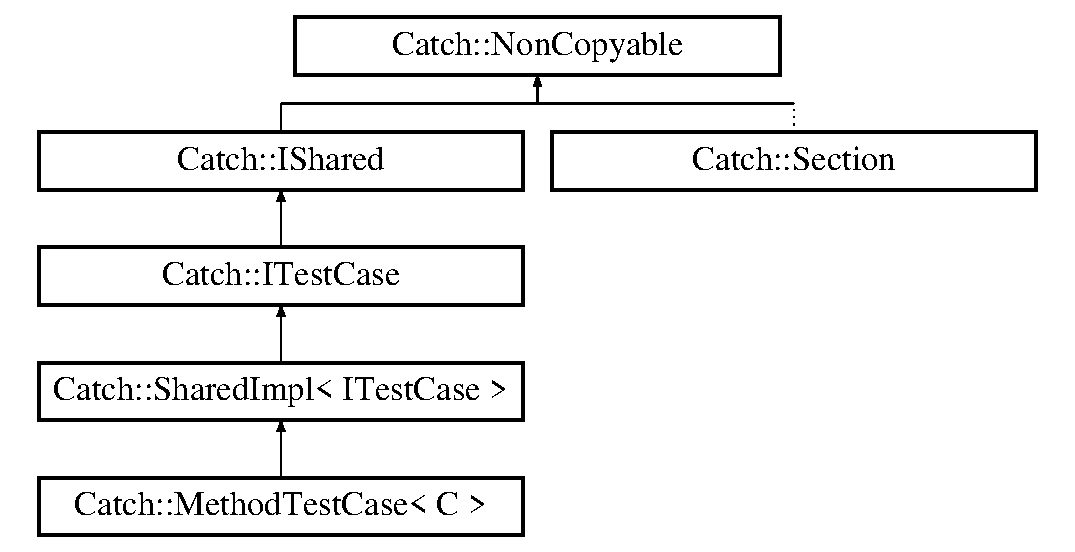
\includegraphics[height=5.000000cm]{classCatch_1_1NonCopyable}
\end{center}
\end{figure}


The documentation for this class was generated from the following file\+:\begin{DoxyCompactItemize}
\item 
test\+\_\+cases/catch.\+hpp\end{DoxyCompactItemize}

\hypertarget{classCatch_1_1NotImplementedException}{}\section{Catch\+:\+:Not\+Implemented\+Exception Class Reference}
\label{classCatch_1_1NotImplementedException}\index{Catch\+::\+Not\+Implemented\+Exception@{Catch\+::\+Not\+Implemented\+Exception}}
Inheritance diagram for Catch\+:\+:Not\+Implemented\+Exception\+:\begin{figure}[H]
\begin{center}
\leavevmode
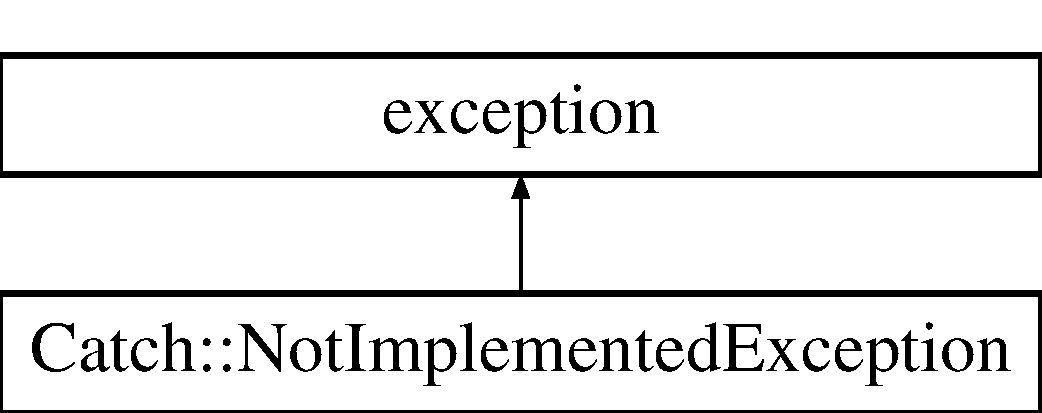
\includegraphics[height=2.000000cm]{classCatch_1_1NotImplementedException}
\end{center}
\end{figure}
\subsection*{Public Member Functions}
\begin{DoxyCompactItemize}
\item 
\mbox{\Hypertarget{classCatch_1_1NotImplementedException_ab4f0a5c39d8ffb72c664e2c07e180634}\label{classCatch_1_1NotImplementedException_ab4f0a5c39d8ffb72c664e2c07e180634}} 
{\bfseries Not\+Implemented\+Exception} (\hyperlink{structCatch_1_1SourceLineInfo}{Source\+Line\+Info} const \&line\+Info)
\item 
\mbox{\Hypertarget{classCatch_1_1NotImplementedException_a508a7a833455da2d3c10ea1a9d45e982}\label{classCatch_1_1NotImplementedException_a508a7a833455da2d3c10ea1a9d45e982}} 
{\bfseries Not\+Implemented\+Exception} (\hyperlink{classCatch_1_1NotImplementedException}{Not\+Implemented\+Exception} const \&)
\item 
\mbox{\Hypertarget{classCatch_1_1NotImplementedException_ad4c13963f1a8feacda0cd331adda89e3}\label{classCatch_1_1NotImplementedException_ad4c13963f1a8feacda0cd331adda89e3}} 
virtual const char $\ast$ {\bfseries what} () const C\+A\+T\+C\+H\+\_\+\+N\+O\+E\+X\+C\+E\+PT
\end{DoxyCompactItemize}


The documentation for this class was generated from the following file\+:\begin{DoxyCompactItemize}
\item 
test\+\_\+cases/catch.\+hpp\end{DoxyCompactItemize}

\hypertarget{classOperationFactory}{}\section{Operation\+Factory Class Reference}
\label{classOperationFactory}\index{Operation\+Factory@{Operation\+Factory}}


{\ttfamily \#include $<$Operation\+Factory.\+h$>$}

\subsection*{Static Public Member Functions}
\begin{DoxyCompactItemize}
\item 
static std\+::shared\+\_\+ptr$<$ \hyperlink{classMarsOperation}{Mars\+Operation} $>$ \hyperlink{classOperationFactory_a97194e25673cefb82196d74091b1d2bf}{create\+Operation} (const string \&data)
\end{DoxyCompactItemize}


\subsection{Detailed Description}
Class managing creating instructions, implementing factory design pattern 

\subsection{Member Function Documentation}
\mbox{\Hypertarget{classOperationFactory_a97194e25673cefb82196d74091b1d2bf}\label{classOperationFactory_a97194e25673cefb82196d74091b1d2bf}} 
\index{Operation\+Factory@{Operation\+Factory}!create\+Operation@{create\+Operation}}
\index{create\+Operation@{create\+Operation}!Operation\+Factory@{Operation\+Factory}}
\subsubsection{\texorpdfstring{create\+Operation()}{createOperation()}}
{\footnotesize\ttfamily std\+::shared\+\_\+ptr$<$ \hyperlink{classMarsOperation}{Mars\+Operation} $>$ Operation\+Factory\+::create\+Operation (\begin{DoxyParamCaption}\item[{const string \&}]{code }\end{DoxyParamCaption})\hspace{0.3cm}{\ttfamily [static]}}

Creates operations 
\begin{DoxyParams}{Parameters}
{\em code} & \hyperlink{classInstruction}{Instruction} code \\
\hline
\end{DoxyParams}
\begin{DoxyReturn}{Returns}
\hyperlink{classMarsOperation}{Mars\+Operation} object of class deduced from code 
\end{DoxyReturn}


The documentation for this class was generated from the following files\+:\begin{DoxyCompactItemize}
\item 
logic/parser/Operation\+Factory.\+h\item 
logic/parser/Operation\+Factory.\+cpp\end{DoxyCompactItemize}

\hypertarget{classOperationParams}{}\section{Operation\+Params Class Reference}
\label{classOperationParams}\index{Operation\+Params@{Operation\+Params}}


{\ttfamily \#include $<$Operation\+Params.\+h$>$}

Inheritance diagram for Operation\+Params\+:\begin{figure}[H]
\begin{center}
\leavevmode
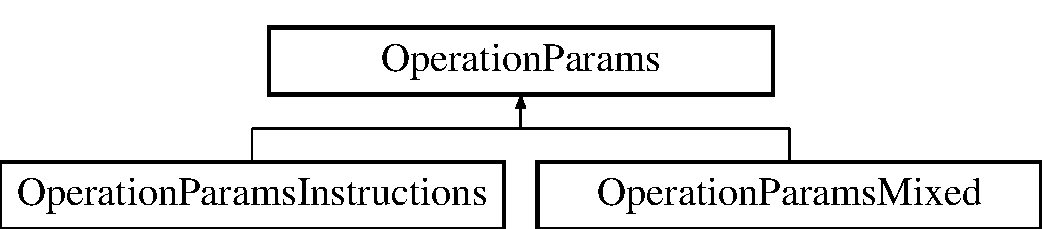
\includegraphics[height=2.000000cm]{classOperationParams}
\end{center}
\end{figure}
\subsection*{Public Member Functions}
\begin{DoxyCompactItemize}
\item 
\mbox{\Hypertarget{classOperationParams_a6753b99754fce0886dbe484d275c3c6a}\label{classOperationParams_a6753b99754fce0886dbe484d275c3c6a}} 
virtual std\+::shared\+\_\+ptr$<$ \hyperlink{classProcessAction}{Process\+Action} $>$ {\bfseries accept} (std\+::shared\+\_\+ptr$<$ \hyperlink{classMarsOperation}{Mars\+Operation} $>$ operation)=0
\end{DoxyCompactItemize}


\subsection{Detailed Description}
Base class representing operation parameters 

The documentation for this class was generated from the following file\+:\begin{DoxyCompactItemize}
\item 
logic/mars/Operation\+Params.\+h\end{DoxyCompactItemize}

\hypertarget{classOperationParamsInstructions}{}\section{Operation\+Params\+Instructions Class Reference}
\label{classOperationParamsInstructions}\index{Operation\+Params\+Instructions@{Operation\+Params\+Instructions}}
Inheritance diagram for Operation\+Params\+Instructions\+:\begin{figure}[H]
\begin{center}
\leavevmode
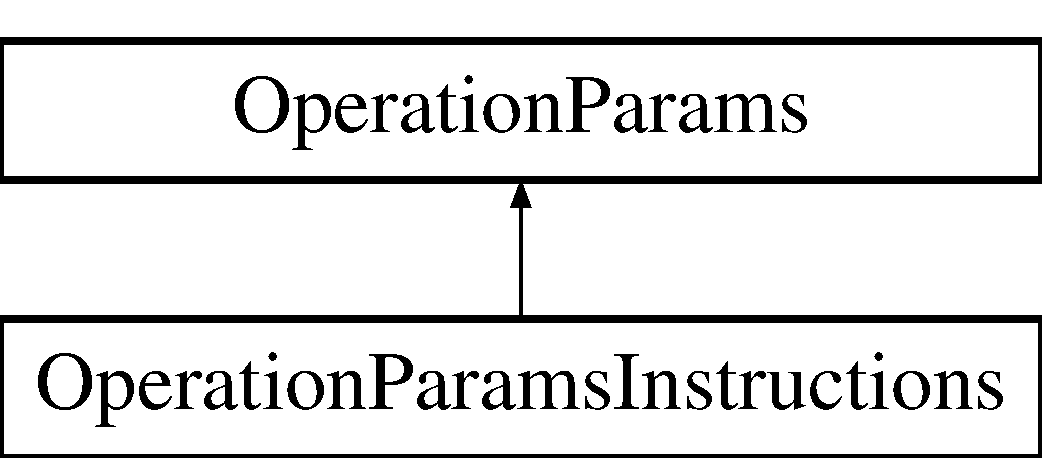
\includegraphics[height=2.000000cm]{classOperationParamsInstructions}
\end{center}
\end{figure}
\subsection*{Public Member Functions}
\begin{DoxyCompactItemize}
\item 
\mbox{\Hypertarget{classOperationParamsInstructions_a49a28c36d1dc02e90f91394f05bd06ec}\label{classOperationParamsInstructions_a49a28c36d1dc02e90f91394f05bd06ec}} 
\hyperlink{classInstruction}{Instruction} \& {\bfseries get\+First\+Instruction} () const
\item 
\mbox{\Hypertarget{classOperationParamsInstructions_a27929107894c47204945f15a80b2e864}\label{classOperationParamsInstructions_a27929107894c47204945f15a80b2e864}} 
\hyperlink{classInstruction}{Instruction} \& {\bfseries get\+Second\+Instruction} () const
\item 
\mbox{\Hypertarget{classOperationParamsInstructions_a6e13df985bf378ead4a0db9164fb4a93}\label{classOperationParamsInstructions_a6e13df985bf378ead4a0db9164fb4a93}} 
{\bfseries Operation\+Params\+Instructions} (\hyperlink{classInstruction}{Instruction} \&instruction\+First, \hyperlink{classInstruction}{Instruction} \&instruction\+Second)
\item 
\mbox{\Hypertarget{classOperationParamsInstructions_ada6b680039d0743fa1ff1a4e638c2301}\label{classOperationParamsInstructions_ada6b680039d0743fa1ff1a4e638c2301}} 
std\+::shared\+\_\+ptr$<$ \hyperlink{classProcessAction}{Process\+Action} $>$ {\bfseries accept} (std\+::shared\+\_\+ptr$<$ \hyperlink{classMarsOperation}{Mars\+Operation} $>$ operation)
\end{DoxyCompactItemize}


The documentation for this class was generated from the following files\+:\begin{DoxyCompactItemize}
\item 
logic/mars/Operation\+Params\+Instructions.\+h\item 
logic/mars/Operation\+Params\+Instructions.\+cpp\end{DoxyCompactItemize}

\hypertarget{classOperationParamsMixed}{}\section{Operation\+Params\+Mixed Class Reference}
\label{classOperationParamsMixed}\index{Operation\+Params\+Mixed@{Operation\+Params\+Mixed}}
Inheritance diagram for Operation\+Params\+Mixed\+:\begin{figure}[H]
\begin{center}
\leavevmode
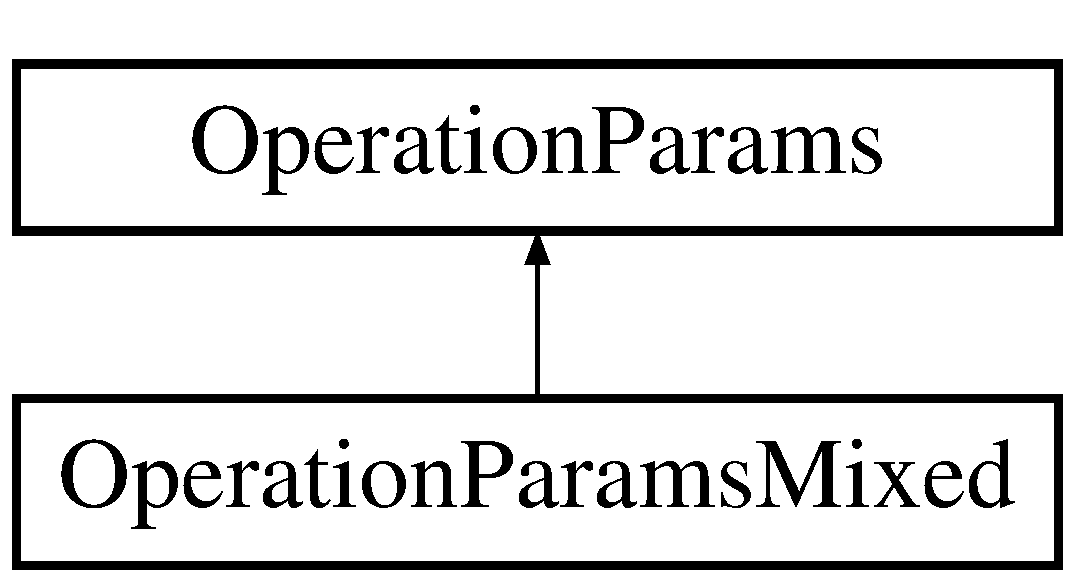
\includegraphics[height=2.000000cm]{classOperationParamsMixed}
\end{center}
\end{figure}
\subsection*{Public Member Functions}
\begin{DoxyCompactItemize}
\item 
\mbox{\Hypertarget{classOperationParamsMixed_ad92325a7406f3e25f2f336a0b5a88010}\label{classOperationParamsMixed_ad92325a7406f3e25f2f336a0b5a88010}} 
{\bfseries Operation\+Params\+Mixed} (int i, \hyperlink{classInstruction}{Instruction} \&instruction)
\item 
\mbox{\Hypertarget{classOperationParamsMixed_ae3df5950117f18772921a40c99a171ad}\label{classOperationParamsMixed_ae3df5950117f18772921a40c99a171ad}} 
int {\bfseries get\+Value} () const
\item 
\mbox{\Hypertarget{classOperationParamsMixed_a292c8725276f1b652e781d0c9e9e4f34}\label{classOperationParamsMixed_a292c8725276f1b652e781d0c9e9e4f34}} 
\hyperlink{classInstruction}{Instruction} \& {\bfseries get\+Instruction} () const
\item 
\mbox{\Hypertarget{classOperationParamsMixed_a44a93f4dc877f4ee1b1deeb83961a519}\label{classOperationParamsMixed_a44a93f4dc877f4ee1b1deeb83961a519}} 
virtual std\+::shared\+\_\+ptr$<$ \hyperlink{classProcessAction}{Process\+Action} $>$ {\bfseries accept} (std\+::shared\+\_\+ptr$<$ \hyperlink{classMarsOperation}{Mars\+Operation} $>$ shared\+\_\+ptr)
\end{DoxyCompactItemize}


The documentation for this class was generated from the following files\+:\begin{DoxyCompactItemize}
\item 
logic/mars/Operation\+Params\+Mixed.\+h\item 
logic/mars/Operation\+Params\+Mixed.\+cpp\end{DoxyCompactItemize}

\hypertarget{structCatch_1_1Internal_1_1OperatorTraits}{}\section{Catch\+:\+:Internal\+:\+:Operator\+Traits$<$ Op $>$ Struct Template Reference}
\label{structCatch_1_1Internal_1_1OperatorTraits}\index{Catch\+::\+Internal\+::\+Operator\+Traits$<$ Op $>$@{Catch\+::\+Internal\+::\+Operator\+Traits$<$ Op $>$}}
\subsection*{Static Public Member Functions}
\begin{DoxyCompactItemize}
\item 
\mbox{\Hypertarget{structCatch_1_1Internal_1_1OperatorTraits_ac6d08082ea33348d42bc4ccbd6d07671}\label{structCatch_1_1Internal_1_1OperatorTraits_ac6d08082ea33348d42bc4ccbd6d07671}} 
static const char $\ast$ {\bfseries get\+Name} ()
\end{DoxyCompactItemize}


The documentation for this struct was generated from the following file\+:\begin{DoxyCompactItemize}
\item 
test\+\_\+cases/catch.\+hpp\end{DoxyCompactItemize}

\hypertarget{structCatch_1_1Internal_1_1OperatorTraits_3_01IsEqualTo_01_4}{}\section{Catch\+:\+:Internal\+:\+:Operator\+Traits$<$ Is\+Equal\+To $>$ Struct Template Reference}
\label{structCatch_1_1Internal_1_1OperatorTraits_3_01IsEqualTo_01_4}\index{Catch\+::\+Internal\+::\+Operator\+Traits$<$ Is\+Equal\+To $>$@{Catch\+::\+Internal\+::\+Operator\+Traits$<$ Is\+Equal\+To $>$}}
\subsection*{Static Public Member Functions}
\begin{DoxyCompactItemize}
\item 
\mbox{\Hypertarget{structCatch_1_1Internal_1_1OperatorTraits_3_01IsEqualTo_01_4_addf03ac66f0ed83abcc037a7a327d4f1}\label{structCatch_1_1Internal_1_1OperatorTraits_3_01IsEqualTo_01_4_addf03ac66f0ed83abcc037a7a327d4f1}} 
static const char $\ast$ {\bfseries get\+Name} ()
\end{DoxyCompactItemize}


The documentation for this struct was generated from the following file\+:\begin{DoxyCompactItemize}
\item 
test\+\_\+cases/catch.\+hpp\end{DoxyCompactItemize}

\hypertarget{structCatch_1_1Internal_1_1OperatorTraits_3_01IsGreaterThan_01_4}{}\section{Catch\+:\+:Internal\+:\+:Operator\+Traits$<$ Is\+Greater\+Than $>$ Struct Template Reference}
\label{structCatch_1_1Internal_1_1OperatorTraits_3_01IsGreaterThan_01_4}\index{Catch\+::\+Internal\+::\+Operator\+Traits$<$ Is\+Greater\+Than $>$@{Catch\+::\+Internal\+::\+Operator\+Traits$<$ Is\+Greater\+Than $>$}}
\subsection*{Static Public Member Functions}
\begin{DoxyCompactItemize}
\item 
\mbox{\Hypertarget{structCatch_1_1Internal_1_1OperatorTraits_3_01IsGreaterThan_01_4_ab917bfb9ccbe461dc684ee5a34d67d27}\label{structCatch_1_1Internal_1_1OperatorTraits_3_01IsGreaterThan_01_4_ab917bfb9ccbe461dc684ee5a34d67d27}} 
static const char $\ast$ {\bfseries get\+Name} ()
\end{DoxyCompactItemize}


The documentation for this struct was generated from the following file\+:\begin{DoxyCompactItemize}
\item 
test\+\_\+cases/catch.\+hpp\end{DoxyCompactItemize}

\hypertarget{structCatch_1_1Internal_1_1OperatorTraits_3_01IsGreaterThanOrEqualTo_01_4}{}\section{Catch\+:\+:Internal\+:\+:Operator\+Traits$<$ Is\+Greater\+Than\+Or\+Equal\+To $>$ Struct Template Reference}
\label{structCatch_1_1Internal_1_1OperatorTraits_3_01IsGreaterThanOrEqualTo_01_4}\index{Catch\+::\+Internal\+::\+Operator\+Traits$<$ Is\+Greater\+Than\+Or\+Equal\+To $>$@{Catch\+::\+Internal\+::\+Operator\+Traits$<$ Is\+Greater\+Than\+Or\+Equal\+To $>$}}
\subsection*{Static Public Member Functions}
\begin{DoxyCompactItemize}
\item 
\mbox{\Hypertarget{structCatch_1_1Internal_1_1OperatorTraits_3_01IsGreaterThanOrEqualTo_01_4_a76b6f6b0dbaf7d19ebb1b4b4891e719e}\label{structCatch_1_1Internal_1_1OperatorTraits_3_01IsGreaterThanOrEqualTo_01_4_a76b6f6b0dbaf7d19ebb1b4b4891e719e}} 
static const char $\ast$ {\bfseries get\+Name} ()
\end{DoxyCompactItemize}


The documentation for this struct was generated from the following file\+:\begin{DoxyCompactItemize}
\item 
test\+\_\+cases/catch.\+hpp\end{DoxyCompactItemize}

\hypertarget{structCatch_1_1Internal_1_1OperatorTraits_3_01IsLessThan_01_4}{}\section{Catch\+:\+:Internal\+:\+:Operator\+Traits$<$ Is\+Less\+Than $>$ Struct Template Reference}
\label{structCatch_1_1Internal_1_1OperatorTraits_3_01IsLessThan_01_4}\index{Catch\+::\+Internal\+::\+Operator\+Traits$<$ Is\+Less\+Than $>$@{Catch\+::\+Internal\+::\+Operator\+Traits$<$ Is\+Less\+Than $>$}}
\subsection*{Static Public Member Functions}
\begin{DoxyCompactItemize}
\item 
\mbox{\Hypertarget{structCatch_1_1Internal_1_1OperatorTraits_3_01IsLessThan_01_4_aa3b536ddbd2e34b1253931ff00c32712}\label{structCatch_1_1Internal_1_1OperatorTraits_3_01IsLessThan_01_4_aa3b536ddbd2e34b1253931ff00c32712}} 
static const char $\ast$ {\bfseries get\+Name} ()
\end{DoxyCompactItemize}


The documentation for this struct was generated from the following file\+:\begin{DoxyCompactItemize}
\item 
test\+\_\+cases/catch.\+hpp\end{DoxyCompactItemize}

\hypertarget{structCatch_1_1Internal_1_1OperatorTraits_3_01IsLessThanOrEqualTo_01_4}{}\section{Catch\+:\+:Internal\+:\+:Operator\+Traits$<$ Is\+Less\+Than\+Or\+Equal\+To $>$ Struct Template Reference}
\label{structCatch_1_1Internal_1_1OperatorTraits_3_01IsLessThanOrEqualTo_01_4}\index{Catch\+::\+Internal\+::\+Operator\+Traits$<$ Is\+Less\+Than\+Or\+Equal\+To $>$@{Catch\+::\+Internal\+::\+Operator\+Traits$<$ Is\+Less\+Than\+Or\+Equal\+To $>$}}
\subsection*{Static Public Member Functions}
\begin{DoxyCompactItemize}
\item 
\mbox{\Hypertarget{structCatch_1_1Internal_1_1OperatorTraits_3_01IsLessThanOrEqualTo_01_4_ae8578813bc847838f10448c1541a9d7b}\label{structCatch_1_1Internal_1_1OperatorTraits_3_01IsLessThanOrEqualTo_01_4_ae8578813bc847838f10448c1541a9d7b}} 
static const char $\ast$ {\bfseries get\+Name} ()
\end{DoxyCompactItemize}


The documentation for this struct was generated from the following file\+:\begin{DoxyCompactItemize}
\item 
test\+\_\+cases/catch.\+hpp\end{DoxyCompactItemize}

\hypertarget{structCatch_1_1Internal_1_1OperatorTraits_3_01IsNotEqualTo_01_4}{}\section{Catch\+:\+:Internal\+:\+:Operator\+Traits$<$ Is\+Not\+Equal\+To $>$ Struct Template Reference}
\label{structCatch_1_1Internal_1_1OperatorTraits_3_01IsNotEqualTo_01_4}\index{Catch\+::\+Internal\+::\+Operator\+Traits$<$ Is\+Not\+Equal\+To $>$@{Catch\+::\+Internal\+::\+Operator\+Traits$<$ Is\+Not\+Equal\+To $>$}}
\subsection*{Static Public Member Functions}
\begin{DoxyCompactItemize}
\item 
\mbox{\Hypertarget{structCatch_1_1Internal_1_1OperatorTraits_3_01IsNotEqualTo_01_4_a54a795b8bf7c80a9fdbc7b81f39133b4}\label{structCatch_1_1Internal_1_1OperatorTraits_3_01IsNotEqualTo_01_4_a54a795b8bf7c80a9fdbc7b81f39133b4}} 
static const char $\ast$ {\bfseries get\+Name} ()
\end{DoxyCompactItemize}


The documentation for this struct was generated from the following file\+:\begin{DoxyCompactItemize}
\item 
test\+\_\+cases/catch.\+hpp\end{DoxyCompactItemize}

\hypertarget{classCatch_1_1Option}{}\section{Catch\+:\+:Option$<$ T $>$ Class Template Reference}
\label{classCatch_1_1Option}\index{Catch\+::\+Option$<$ T $>$@{Catch\+::\+Option$<$ T $>$}}
\subsection*{Public Member Functions}
\begin{DoxyCompactItemize}
\item 
\mbox{\Hypertarget{classCatch_1_1Option_a5aeb9c22d48a6882bdf5fb4730b06c86}\label{classCatch_1_1Option_a5aeb9c22d48a6882bdf5fb4730b06c86}} 
{\bfseries Option} (T const \&\+\_\+value)
\item 
\mbox{\Hypertarget{classCatch_1_1Option_af02f2e4559f06384baec0def8c68c5fd}\label{classCatch_1_1Option_af02f2e4559f06384baec0def8c68c5fd}} 
{\bfseries Option} (\hyperlink{classCatch_1_1Option}{Option} const \&\+\_\+other)
\item 
\mbox{\Hypertarget{classCatch_1_1Option_a78c65b15dd6b2fbd04c5012c43017c8f}\label{classCatch_1_1Option_a78c65b15dd6b2fbd04c5012c43017c8f}} 
\hyperlink{classCatch_1_1Option}{Option} \& {\bfseries operator=} (\hyperlink{classCatch_1_1Option}{Option} const \&\+\_\+other)
\item 
\mbox{\Hypertarget{classCatch_1_1Option_a2be7e343ab22d6061726d32ab4622653}\label{classCatch_1_1Option_a2be7e343ab22d6061726d32ab4622653}} 
\hyperlink{classCatch_1_1Option}{Option} \& {\bfseries operator=} (T const \&\+\_\+value)
\item 
\mbox{\Hypertarget{classCatch_1_1Option_a37b4e0e5d4d56296adacd267a616f4e0}\label{classCatch_1_1Option_a37b4e0e5d4d56296adacd267a616f4e0}} 
void {\bfseries reset} ()
\item 
\mbox{\Hypertarget{classCatch_1_1Option_afd989852fa453731c3190dac63caccb0}\label{classCatch_1_1Option_afd989852fa453731c3190dac63caccb0}} 
T \& {\bfseries operator$\ast$} ()
\item 
\mbox{\Hypertarget{classCatch_1_1Option_a734fc9c2eb1a1f7f8e8f6a4eb12160f0}\label{classCatch_1_1Option_a734fc9c2eb1a1f7f8e8f6a4eb12160f0}} 
T const  \& {\bfseries operator$\ast$} () const
\item 
\mbox{\Hypertarget{classCatch_1_1Option_acad340798a16c8f700f8763119e90f31}\label{classCatch_1_1Option_acad340798a16c8f700f8763119e90f31}} 
T $\ast$ {\bfseries operator-\/$>$} ()
\item 
\mbox{\Hypertarget{classCatch_1_1Option_ae8343cbc36dbb95b2dce333d2a6fdc28}\label{classCatch_1_1Option_ae8343cbc36dbb95b2dce333d2a6fdc28}} 
const T $\ast$ {\bfseries operator-\/$>$} () const
\item 
\mbox{\Hypertarget{classCatch_1_1Option_a8d9ae2e30b0eb76fe134a6fbc8423124}\label{classCatch_1_1Option_a8d9ae2e30b0eb76fe134a6fbc8423124}} 
T {\bfseries value\+Or} (T const \&default\+Value) const
\item 
\mbox{\Hypertarget{classCatch_1_1Option_a97c95829afbe92f2bcc5fd75b32c0825}\label{classCatch_1_1Option_a97c95829afbe92f2bcc5fd75b32c0825}} 
bool {\bfseries some} () const
\item 
\mbox{\Hypertarget{classCatch_1_1Option_a821753afdc3fac947a13a01fbe0d248e}\label{classCatch_1_1Option_a821753afdc3fac947a13a01fbe0d248e}} 
bool {\bfseries none} () const
\item 
\mbox{\Hypertarget{classCatch_1_1Option_a96dccb86bdf45ee0c08e122b6133bef3}\label{classCatch_1_1Option_a96dccb86bdf45ee0c08e122b6133bef3}} 
bool {\bfseries operator!} () const
\item 
\mbox{\Hypertarget{classCatch_1_1Option_a8ed8de7b072f893c85df14913dbbe197}\label{classCatch_1_1Option_a8ed8de7b072f893c85df14913dbbe197}} 
{\bfseries operator Safe\+Bool\+::type} () const
\end{DoxyCompactItemize}


The documentation for this class was generated from the following file\+:\begin{DoxyCompactItemize}
\item 
test\+\_\+cases/catch.\+hpp\end{DoxyCompactItemize}

\hypertarget{classParserException}{}\section{Parser\+Exception Class Reference}
\label{classParserException}\index{Parser\+Exception@{Parser\+Exception}}


{\ttfamily \#include $<$Parser\+Exception.\+h$>$}

Inheritance diagram for Parser\+Exception\+:\begin{figure}[H]
\begin{center}
\leavevmode
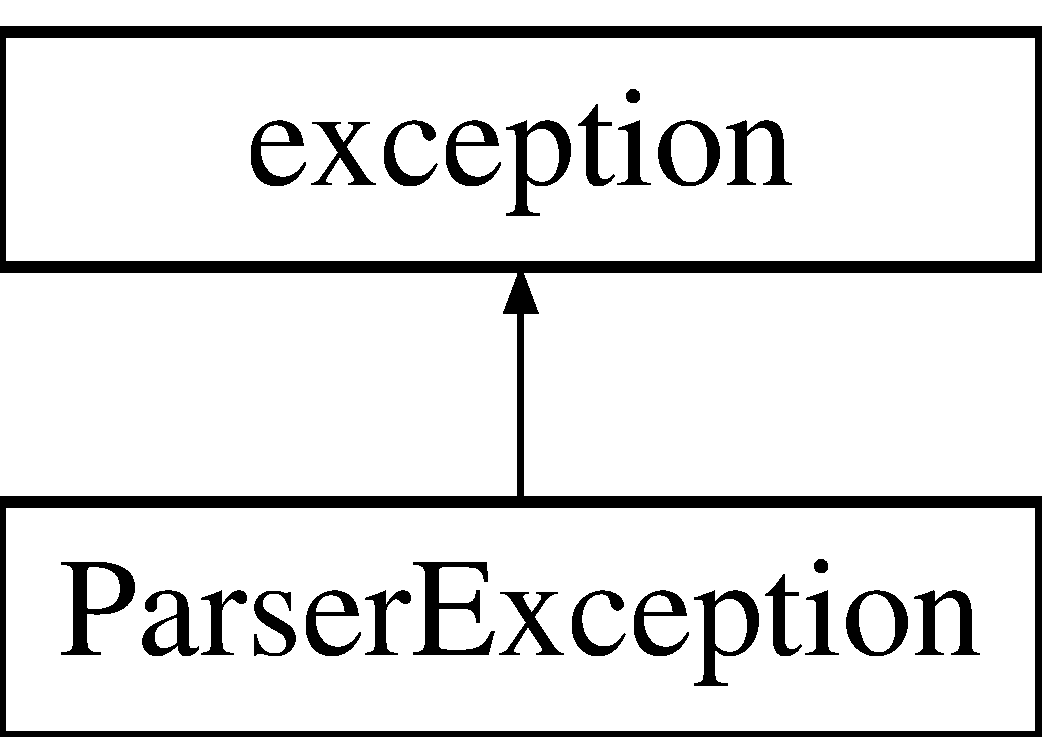
\includegraphics[height=2.000000cm]{classParserException}
\end{center}
\end{figure}
\subsection*{Public Member Functions}
\begin{DoxyCompactItemize}
\item 
\mbox{\Hypertarget{classParserException_a2fb349add0a7c46a7cd67779230a2ed2}\label{classParserException_a2fb349add0a7c46a7cd67779230a2ed2}} 
{\bfseries Parser\+Exception} (const std\+::string \&message)
\item 
\mbox{\Hypertarget{classParserException_a3b07178ab4d1f19888379e618571bf71}\label{classParserException_a3b07178ab4d1f19888379e618571bf71}} 
const char $\ast$ {\bfseries what} () const noexcept override
\end{DoxyCompactItemize}
\subsection*{Protected Attributes}
\begin{DoxyCompactItemize}
\item 
\mbox{\Hypertarget{classParserException_a1a45989b6dfdaf8bf4798a74dbeb2b4a}\label{classParserException_a1a45989b6dfdaf8bf4798a74dbeb2b4a}} 
std\+::string {\bfseries message}
\end{DoxyCompactItemize}


\subsection{Detailed Description}
Parser exception class 

The documentation for this class was generated from the following files\+:\begin{DoxyCompactItemize}
\item 
logic/parser/Parser\+Exception.\+h\item 
logic/parser/Parser\+Exception.\+cpp\end{DoxyCompactItemize}

\hypertarget{classPlayer}{}\section{Player Class Reference}
\label{classPlayer}\index{Player@{Player}}
\subsection*{Public Member Functions}
\begin{DoxyCompactItemize}
\item 
\mbox{\Hypertarget{classPlayer_a618464c7f53560e3abbfd7f259135221}\label{classPlayer_a618464c7f53560e3abbfd7f259135221}} 
{\bfseries Player} (\hyperlink{classPlayerInfo}{Player\+Info} \&info)
\item 
\mbox{\Hypertarget{classPlayer_a7d46e5528dc9afbe4c8b2c0823b95813}\label{classPlayer_a7d46e5528dc9afbe4c8b2c0823b95813}} 
void {\bfseries test} () const
\end{DoxyCompactItemize}


The documentation for this class was generated from the following files\+:\begin{DoxyCompactItemize}
\item 
logic/Player.\+h\item 
logic/Player.\+cpp\end{DoxyCompactItemize}

\hypertarget{classPlayerCreator}{}\section{Player\+Creator Class Reference}
\label{classPlayerCreator}\index{Player\+Creator@{Player\+Creator}}
\subsection*{Static Public Member Functions}
\begin{DoxyCompactItemize}
\item 
static std\+::vector$<$ \hyperlink{classPlayer}{Player} $>$ \hyperlink{classPlayerCreator_a67fe8a11ac468ecb1f82391a65252360}{create\+Players} (std\+::vector$<$ \hyperlink{classViewInput}{View\+Input} $>$)
\end{DoxyCompactItemize}


\subsection{Member Function Documentation}
\mbox{\Hypertarget{classPlayerCreator_a67fe8a11ac468ecb1f82391a65252360}\label{classPlayerCreator_a67fe8a11ac468ecb1f82391a65252360}} 
\index{Player\+Creator@{Player\+Creator}!create\+Players@{create\+Players}}
\index{create\+Players@{create\+Players}!Player\+Creator@{Player\+Creator}}
\subsubsection{\texorpdfstring{create\+Players()}{createPlayers()}}
{\footnotesize\ttfamily std\+::vector$<$ \hyperlink{classPlayer}{Player} $>$ Player\+Creator\+::create\+Players (\begin{DoxyParamCaption}\item[{std\+::vector$<$ \hyperlink{classViewInput}{View\+Input} $>$}]{inputs }\end{DoxyParamCaption})\hspace{0.3cm}{\ttfamily [static]}}


\begin{DoxyParams}{Parameters}
{\em inputs} & \\
\hline
\end{DoxyParams}
\begin{DoxyReturn}{Returns}

\end{DoxyReturn}


The documentation for this class was generated from the following files\+:\begin{DoxyCompactItemize}
\item 
logic/Player\+Creator.\+h\item 
logic/Player\+Creator.\+cpp\end{DoxyCompactItemize}

\hypertarget{classPlayerInfo}{}\section{Player\+Info Class Reference}
\label{classPlayerInfo}\index{Player\+Info@{Player\+Info}}
\subsection*{Public Member Functions}
\begin{DoxyCompactItemize}
\item 
\mbox{\Hypertarget{classPlayerInfo_add5236b33c036a382f9032dac6196af4}\label{classPlayerInfo_add5236b33c036a382f9032dac6196af4}} 
{\bfseries Player\+Info} (std\+::string \&basic\+\_\+string)
\end{DoxyCompactItemize}


The documentation for this class was generated from the following files\+:\begin{DoxyCompactItemize}
\item 
logic/Player\+Info.\+h\item 
logic/Player\+Info.\+cpp\end{DoxyCompactItemize}

\hypertarget{structCatch_1_1pluralise}{}\section{Catch\+:\+:pluralise Struct Reference}
\label{structCatch_1_1pluralise}\index{Catch\+::pluralise@{Catch\+::pluralise}}
\subsection*{Public Member Functions}
\begin{DoxyCompactItemize}
\item 
\mbox{\Hypertarget{structCatch_1_1pluralise_a5c55e22de2416cfe416edf715c6b9234}\label{structCatch_1_1pluralise_a5c55e22de2416cfe416edf715c6b9234}} 
{\bfseries pluralise} (std\+::size\+\_\+t count, std\+::string const \&label)
\end{DoxyCompactItemize}
\subsection*{Public Attributes}
\begin{DoxyCompactItemize}
\item 
\mbox{\Hypertarget{structCatch_1_1pluralise_a4dce2fa13ec6f00fac09b2418265441e}\label{structCatch_1_1pluralise_a4dce2fa13ec6f00fac09b2418265441e}} 
std\+::size\+\_\+t {\bfseries m\+\_\+count}
\item 
\mbox{\Hypertarget{structCatch_1_1pluralise_a8849cbdd3f11ebe7747597c8644e8793}\label{structCatch_1_1pluralise_a8849cbdd3f11ebe7747597c8644e8793}} 
std\+::string {\bfseries m\+\_\+label}
\end{DoxyCompactItemize}
\subsection*{Friends}
\begin{DoxyCompactItemize}
\item 
\mbox{\Hypertarget{structCatch_1_1pluralise_aa7dac6b165514c1f85e0695d678fdef5}\label{structCatch_1_1pluralise_aa7dac6b165514c1f85e0695d678fdef5}} 
std\+::ostream \& {\bfseries operator$<$$<$} (std\+::ostream \&os, \hyperlink{structCatch_1_1pluralise}{pluralise} const \&pluraliser)
\end{DoxyCompactItemize}


The documentation for this struct was generated from the following file\+:\begin{DoxyCompactItemize}
\item 
test\+\_\+cases/catch.\+hpp\end{DoxyCompactItemize}

\hypertarget{classProcessAction}{}\section{Process\+Action Class Reference}
\label{classProcessAction}\index{Process\+Action@{Process\+Action}}
Inheritance diagram for Process\+Action\+:\begin{figure}[H]
\begin{center}
\leavevmode
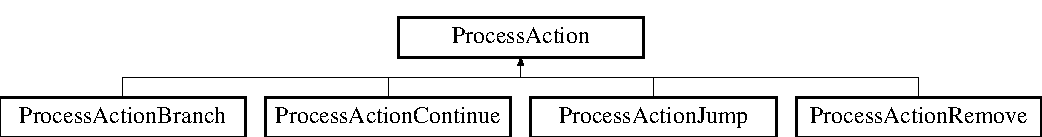
\includegraphics[height=1.842105cm]{classProcessAction}
\end{center}
\end{figure}
\subsection*{Public Member Functions}
\begin{DoxyCompactItemize}
\item 
\mbox{\Hypertarget{classProcessAction_a74bf3c774520f3c6deb1e0fc09278415}\label{classProcessAction_a74bf3c774520f3c6deb1e0fc09278415}} 
virtual void {\bfseries run\+Action} (\hyperlink{classProcessManager}{Process\+Manager} \&pm)=0
\end{DoxyCompactItemize}


The documentation for this class was generated from the following file\+:\begin{DoxyCompactItemize}
\item 
logic/mars/Process\+Action.\+h\end{DoxyCompactItemize}

\hypertarget{classProcessActionBranch}{}\section{Process\+Action\+Branch Class Reference}
\label{classProcessActionBranch}\index{Process\+Action\+Branch@{Process\+Action\+Branch}}
Inheritance diagram for Process\+Action\+Branch\+:\begin{figure}[H]
\begin{center}
\leavevmode
\includegraphics[height=2.000000cm]{classProcessActionBranch}
\end{center}
\end{figure}
\subsection*{Public Member Functions}
\begin{DoxyCompactItemize}
\item 
\mbox{\Hypertarget{classProcessActionBranch_af07066ed151e010ed2231436c98bb0b7}\label{classProcessActionBranch_af07066ed151e010ed2231436c98bb0b7}} 
{\bfseries Process\+Action\+Branch} (int branch\+Address)
\item 
\hyperlink{classMemoryIndex}{Memory\+Index} \hyperlink{classProcessActionBranch_a692987ed51a14885871a55cd08a994f0}{get\+Branch\+Address} () const
\item 
virtual void \hyperlink{classProcessActionBranch_a2aadd61680b350a4b9112ff3757f1944}{run\+Action} (\hyperlink{classProcessManager}{Process\+Manager} \&manager) override
\end{DoxyCompactItemize}


\subsection{Member Function Documentation}
\mbox{\Hypertarget{classProcessActionBranch_a692987ed51a14885871a55cd08a994f0}\label{classProcessActionBranch_a692987ed51a14885871a55cd08a994f0}} 
\index{Process\+Action\+Branch@{Process\+Action\+Branch}!get\+Branch\+Address@{get\+Branch\+Address}}
\index{get\+Branch\+Address@{get\+Branch\+Address}!Process\+Action\+Branch@{Process\+Action\+Branch}}
\subsubsection{\texorpdfstring{get\+Branch\+Address()}{getBranchAddress()}}
{\footnotesize\ttfamily \hyperlink{classMemoryIndex}{Memory\+Index} Process\+Action\+Branch\+::get\+Branch\+Address (\begin{DoxyParamCaption}{ }\end{DoxyParamCaption}) const}

Returns branch address \begin{DoxyReturn}{Returns}
branch\+Address 
\end{DoxyReturn}
\mbox{\Hypertarget{classProcessActionBranch_a2aadd61680b350a4b9112ff3757f1944}\label{classProcessActionBranch_a2aadd61680b350a4b9112ff3757f1944}} 
\index{Process\+Action\+Branch@{Process\+Action\+Branch}!run\+Action@{run\+Action}}
\index{run\+Action@{run\+Action}!Process\+Action\+Branch@{Process\+Action\+Branch}}
\subsubsection{\texorpdfstring{run\+Action()}{runAction()}}
{\footnotesize\ttfamily void Process\+Action\+Branch\+::run\+Action (\begin{DoxyParamCaption}\item[{\hyperlink{classProcessManager}{Process\+Manager} \&}]{manager }\end{DoxyParamCaption})\hspace{0.3cm}{\ttfamily [override]}, {\ttfamily [virtual]}}

Branches current instruction 
\begin{DoxyParams}{Parameters}
{\em manager} & \\
\hline
\end{DoxyParams}


Implements \hyperlink{classProcessAction}{Process\+Action}.



The documentation for this class was generated from the following files\+:\begin{DoxyCompactItemize}
\item 
logic/mars/Process\+Action\+Branch.\+h\item 
logic/mars/Process\+Action\+Branch.\+cpp\end{DoxyCompactItemize}

\hypertarget{classProcessActionContinue}{}\section{Process\+Action\+Continue Class Reference}
\label{classProcessActionContinue}\index{Process\+Action\+Continue@{Process\+Action\+Continue}}
Inheritance diagram for Process\+Action\+Continue\+:\begin{figure}[H]
\begin{center}
\leavevmode
\includegraphics[height=2.000000cm]{classProcessActionContinue}
\end{center}
\end{figure}
\subsection*{Public Member Functions}
\begin{DoxyCompactItemize}
\item 
virtual void \hyperlink{classProcessActionContinue_a5ed33d879b9caaf8c94ac5703696eb48}{run\+Action} (\hyperlink{classProcessManager}{Process\+Manager} \&manager) override
\end{DoxyCompactItemize}


\subsection{Member Function Documentation}
\mbox{\Hypertarget{classProcessActionContinue_a5ed33d879b9caaf8c94ac5703696eb48}\label{classProcessActionContinue_a5ed33d879b9caaf8c94ac5703696eb48}} 
\index{Process\+Action\+Continue@{Process\+Action\+Continue}!run\+Action@{run\+Action}}
\index{run\+Action@{run\+Action}!Process\+Action\+Continue@{Process\+Action\+Continue}}
\subsubsection{\texorpdfstring{run\+Action()}{runAction()}}
{\footnotesize\ttfamily void Process\+Action\+Continue\+::run\+Action (\begin{DoxyParamCaption}\item[{\hyperlink{classProcessManager}{Process\+Manager} \&}]{manager }\end{DoxyParamCaption})\hspace{0.3cm}{\ttfamily [override]}, {\ttfamily [virtual]}}

Proceeds to next instruction 
\begin{DoxyParams}{Parameters}
{\em manager} & \\
\hline
\end{DoxyParams}


Implements \hyperlink{classProcessAction}{Process\+Action}.



The documentation for this class was generated from the following files\+:\begin{DoxyCompactItemize}
\item 
logic/mars/Process\+Action\+Continue.\+h\item 
logic/mars/Process\+Action\+Continue.\+cpp\end{DoxyCompactItemize}

\hypertarget{classProcessActionJump}{}\section{Process\+Action\+Jump Class Reference}
\label{classProcessActionJump}\index{Process\+Action\+Jump@{Process\+Action\+Jump}}
Inheritance diagram for Process\+Action\+Jump\+:\begin{figure}[H]
\begin{center}
\leavevmode
\includegraphics[height=2.000000cm]{classProcessActionJump}
\end{center}
\end{figure}
\subsection*{Public Member Functions}
\begin{DoxyCompactItemize}
\item 
\mbox{\Hypertarget{classProcessActionJump_ab2d4c7e11b65b3010cb7be96c454820b}\label{classProcessActionJump_ab2d4c7e11b65b3010cb7be96c454820b}} 
{\bfseries Process\+Action\+Jump} (int jump)
\item 
int \hyperlink{classProcessActionJump_a196bb3613ab7a51d2ff07edf757a8d6a}{get\+Jump\+Value} () const
\item 
virtual void \hyperlink{classProcessActionJump_a655f264451f08675b094a38fcb540155}{run\+Action} (\hyperlink{classProcessManager}{Process\+Manager} \&manager) override
\end{DoxyCompactItemize}


\subsection{Member Function Documentation}
\mbox{\Hypertarget{classProcessActionJump_a196bb3613ab7a51d2ff07edf757a8d6a}\label{classProcessActionJump_a196bb3613ab7a51d2ff07edf757a8d6a}} 
\index{Process\+Action\+Jump@{Process\+Action\+Jump}!get\+Jump\+Value@{get\+Jump\+Value}}
\index{get\+Jump\+Value@{get\+Jump\+Value}!Process\+Action\+Jump@{Process\+Action\+Jump}}
\subsubsection{\texorpdfstring{get\+Jump\+Value()}{getJumpValue()}}
{\footnotesize\ttfamily int Process\+Action\+Jump\+::get\+Jump\+Value (\begin{DoxyParamCaption}{ }\end{DoxyParamCaption}) const}

Returns jump value \begin{DoxyReturn}{Returns}
jump\+Value 
\end{DoxyReturn}
\mbox{\Hypertarget{classProcessActionJump_a655f264451f08675b094a38fcb540155}\label{classProcessActionJump_a655f264451f08675b094a38fcb540155}} 
\index{Process\+Action\+Jump@{Process\+Action\+Jump}!run\+Action@{run\+Action}}
\index{run\+Action@{run\+Action}!Process\+Action\+Jump@{Process\+Action\+Jump}}
\subsubsection{\texorpdfstring{run\+Action()}{runAction()}}
{\footnotesize\ttfamily void Process\+Action\+Jump\+::run\+Action (\begin{DoxyParamCaption}\item[{\hyperlink{classProcessManager}{Process\+Manager} \&}]{manager }\end{DoxyParamCaption})\hspace{0.3cm}{\ttfamily [override]}, {\ttfamily [virtual]}}

Jumps jump\+Value instructions ahead 
\begin{DoxyParams}{Parameters}
{\em manager} & \\
\hline
\end{DoxyParams}


Implements \hyperlink{classProcessAction}{Process\+Action}.



The documentation for this class was generated from the following files\+:\begin{DoxyCompactItemize}
\item 
logic/mars/Process\+Action\+Jump.\+h\item 
logic/mars/Process\+Action\+Jump.\+cpp\end{DoxyCompactItemize}

\hypertarget{classProcessActionRemove}{}\section{Process\+Action\+Remove Class Reference}
\label{classProcessActionRemove}\index{Process\+Action\+Remove@{Process\+Action\+Remove}}
Inheritance diagram for Process\+Action\+Remove\+:\begin{figure}[H]
\begin{center}
\leavevmode
\includegraphics[height=2.000000cm]{classProcessActionRemove}
\end{center}
\end{figure}
\subsection*{Public Member Functions}
\begin{DoxyCompactItemize}
\item 
virtual void \hyperlink{classProcessActionRemove_ac673f99819ee50b724277f02005f3f39}{run\+Action} (\hyperlink{classProcessManager}{Process\+Manager} \&manager) override
\end{DoxyCompactItemize}


\subsection{Member Function Documentation}
\mbox{\Hypertarget{classProcessActionRemove_ac673f99819ee50b724277f02005f3f39}\label{classProcessActionRemove_ac673f99819ee50b724277f02005f3f39}} 
\index{Process\+Action\+Remove@{Process\+Action\+Remove}!run\+Action@{run\+Action}}
\index{run\+Action@{run\+Action}!Process\+Action\+Remove@{Process\+Action\+Remove}}
\subsubsection{\texorpdfstring{run\+Action()}{runAction()}}
{\footnotesize\ttfamily void Process\+Action\+Remove\+::run\+Action (\begin{DoxyParamCaption}\item[{\hyperlink{classProcessManager}{Process\+Manager} \&}]{manager }\end{DoxyParamCaption})\hspace{0.3cm}{\ttfamily [override]}, {\ttfamily [virtual]}}

Removes current instruction 
\begin{DoxyParams}{Parameters}
{\em manager} & Process manager object reference \\
\hline
\end{DoxyParams}


Implements \hyperlink{classProcessAction}{Process\+Action}.



The documentation for this class was generated from the following files\+:\begin{DoxyCompactItemize}
\item 
logic/mars/Process\+Action\+Remove.\+h\item 
logic/mars/Process\+Action\+Remove.\+cpp\end{DoxyCompactItemize}

\hypertarget{classProcessManager}{}\section{Process\+Manager Class Reference}
\label{classProcessManager}\index{Process\+Manager@{Process\+Manager}}


{\ttfamily \#include $<$Process\+Manager.\+h$>$}

\subsection*{Public Member Functions}
\begin{DoxyCompactItemize}
\item 
\hyperlink{classProcessManager_ae180ab47bde18fe2879a8d7473c1a80c}{Process\+Manager} (int first\+Process)
\item 
\hyperlink{classProcessManager_ab8b145c5552462cbeb1b81cf085ac694}{Process\+Manager} (\hyperlink{classMemoryIndex}{Memory\+Index} first\+Process)
\item 
void \hyperlink{classProcessManager_a3a526dfc1413064125c163e58411070d}{jump\+Over} (int i)
\item 
void \hyperlink{classProcessManager_ad1050286f389fc52063ac4fb29fa8020}{proceed\+To\+Next\+Instruction} ()
\item 
void \hyperlink{classProcessManager_a7e9a444c31df1147142843da620ffecd}{remove\+Current\+Instruction} ()
\item 
void \hyperlink{classProcessManager_ac2cbf900825382675f11911098fa0f66}{branch\+Current\+Instruction} (\hyperlink{classMemoryIndex}{Memory\+Index} branch\+Address)
\item 
void \hyperlink{classProcessManager_a2aaeb45b6e1a58e86856899d925c2c7f}{jump\+From\+Current\+Instruction} (int jump\+Value)
\item 
\hyperlink{classMemoryIndex}{Memory\+Index} \hyperlink{classProcessManager_abfb4edde7c0650b0bfc457a5be28d514}{get\+Current\+Address} ()
\item 
int \hyperlink{classProcessManager_a20de7626ee3409fb05c0b53a32697bae}{get\+Size} ()
\end{DoxyCompactItemize}


\subsection{Detailed Description}
Class for managing processes 

\subsection{Constructor \& Destructor Documentation}
\mbox{\Hypertarget{classProcessManager_ae180ab47bde18fe2879a8d7473c1a80c}\label{classProcessManager_ae180ab47bde18fe2879a8d7473c1a80c}} 
\index{Process\+Manager@{Process\+Manager}!Process\+Manager@{Process\+Manager}}
\index{Process\+Manager@{Process\+Manager}!Process\+Manager@{Process\+Manager}}
\subsubsection{\texorpdfstring{Process\+Manager()}{ProcessManager()}\hspace{0.1cm}{\footnotesize\ttfamily [1/2]}}
{\footnotesize\ttfamily Process\+Manager\+::\+Process\+Manager (\begin{DoxyParamCaption}\item[{int}]{first\+Process }\end{DoxyParamCaption})}

Creates and adds process 
\begin{DoxyParams}{Parameters}
{\em first\+Process} & \\
\hline
\end{DoxyParams}
\mbox{\Hypertarget{classProcessManager_ab8b145c5552462cbeb1b81cf085ac694}\label{classProcessManager_ab8b145c5552462cbeb1b81cf085ac694}} 
\index{Process\+Manager@{Process\+Manager}!Process\+Manager@{Process\+Manager}}
\index{Process\+Manager@{Process\+Manager}!Process\+Manager@{Process\+Manager}}
\subsubsection{\texorpdfstring{Process\+Manager()}{ProcessManager()}\hspace{0.1cm}{\footnotesize\ttfamily [2/2]}}
{\footnotesize\ttfamily Process\+Manager\+::\+Process\+Manager (\begin{DoxyParamCaption}\item[{\hyperlink{classMemoryIndex}{Memory\+Index}}]{first\+Process }\end{DoxyParamCaption})}

Adds process 
\begin{DoxyParams}{Parameters}
{\em first\+Process} & \\
\hline
\end{DoxyParams}


\subsection{Member Function Documentation}
\mbox{\Hypertarget{classProcessManager_ac2cbf900825382675f11911098fa0f66}\label{classProcessManager_ac2cbf900825382675f11911098fa0f66}} 
\index{Process\+Manager@{Process\+Manager}!branch\+Current\+Instruction@{branch\+Current\+Instruction}}
\index{branch\+Current\+Instruction@{branch\+Current\+Instruction}!Process\+Manager@{Process\+Manager}}
\subsubsection{\texorpdfstring{branch\+Current\+Instruction()}{branchCurrentInstruction()}}
{\footnotesize\ttfamily void Process\+Manager\+::branch\+Current\+Instruction (\begin{DoxyParamCaption}\item[{\hyperlink{classMemoryIndex}{Memory\+Index}}]{branch\+Address }\end{DoxyParamCaption})}

Starts a new process from address branch\+Address 
\begin{DoxyParams}{Parameters}
{\em branch\+Address} & address of new process \\
\hline
\end{DoxyParams}
\mbox{\Hypertarget{classProcessManager_abfb4edde7c0650b0bfc457a5be28d514}\label{classProcessManager_abfb4edde7c0650b0bfc457a5be28d514}} 
\index{Process\+Manager@{Process\+Manager}!get\+Current\+Address@{get\+Current\+Address}}
\index{get\+Current\+Address@{get\+Current\+Address}!Process\+Manager@{Process\+Manager}}
\subsubsection{\texorpdfstring{get\+Current\+Address()}{getCurrentAddress()}}
{\footnotesize\ttfamily \hyperlink{classMemoryIndex}{Memory\+Index} Process\+Manager\+::get\+Current\+Address (\begin{DoxyParamCaption}{ }\end{DoxyParamCaption})}

Returns address of current process \begin{DoxyReturn}{Returns}

\end{DoxyReturn}
\mbox{\Hypertarget{classProcessManager_a20de7626ee3409fb05c0b53a32697bae}\label{classProcessManager_a20de7626ee3409fb05c0b53a32697bae}} 
\index{Process\+Manager@{Process\+Manager}!get\+Size@{get\+Size}}
\index{get\+Size@{get\+Size}!Process\+Manager@{Process\+Manager}}
\subsubsection{\texorpdfstring{get\+Size()}{getSize()}}
{\footnotesize\ttfamily int Process\+Manager\+::get\+Size (\begin{DoxyParamCaption}{ }\end{DoxyParamCaption})}

Returns number of processes \begin{DoxyReturn}{Returns}
number of processes 
\end{DoxyReturn}
\mbox{\Hypertarget{classProcessManager_a2aaeb45b6e1a58e86856899d925c2c7f}\label{classProcessManager_a2aaeb45b6e1a58e86856899d925c2c7f}} 
\index{Process\+Manager@{Process\+Manager}!jump\+From\+Current\+Instruction@{jump\+From\+Current\+Instruction}}
\index{jump\+From\+Current\+Instruction@{jump\+From\+Current\+Instruction}!Process\+Manager@{Process\+Manager}}
\subsubsection{\texorpdfstring{jump\+From\+Current\+Instruction()}{jumpFromCurrentInstruction()}}
{\footnotesize\ttfamily void Process\+Manager\+::jump\+From\+Current\+Instruction (\begin{DoxyParamCaption}\item[{int}]{jump\+Value }\end{DoxyParamCaption})}

Jumps jump\+Value instructions forward 
\begin{DoxyParams}{Parameters}
{\em jump\+Value} & \\
\hline
\end{DoxyParams}
\mbox{\Hypertarget{classProcessManager_a3a526dfc1413064125c163e58411070d}\label{classProcessManager_a3a526dfc1413064125c163e58411070d}} 
\index{Process\+Manager@{Process\+Manager}!jump\+Over@{jump\+Over}}
\index{jump\+Over@{jump\+Over}!Process\+Manager@{Process\+Manager}}
\subsubsection{\texorpdfstring{jump\+Over()}{jumpOver()}}
{\footnotesize\ttfamily void Process\+Manager\+::jump\+Over (\begin{DoxyParamCaption}\item[{int}]{i }\end{DoxyParamCaption})}

Jumps i instructions ahead 
\begin{DoxyParams}{Parameters}
{\em i} & number of instructions to jump over \\
\hline
\end{DoxyParams}
\mbox{\Hypertarget{classProcessManager_ad1050286f389fc52063ac4fb29fa8020}\label{classProcessManager_ad1050286f389fc52063ac4fb29fa8020}} 
\index{Process\+Manager@{Process\+Manager}!proceed\+To\+Next\+Instruction@{proceed\+To\+Next\+Instruction}}
\index{proceed\+To\+Next\+Instruction@{proceed\+To\+Next\+Instruction}!Process\+Manager@{Process\+Manager}}
\subsubsection{\texorpdfstring{proceed\+To\+Next\+Instruction()}{proceedToNextInstruction()}}
{\footnotesize\ttfamily void Process\+Manager\+::proceed\+To\+Next\+Instruction (\begin{DoxyParamCaption}{ }\end{DoxyParamCaption})}

Skips to next instruction \mbox{\Hypertarget{classProcessManager_a7e9a444c31df1147142843da620ffecd}\label{classProcessManager_a7e9a444c31df1147142843da620ffecd}} 
\index{Process\+Manager@{Process\+Manager}!remove\+Current\+Instruction@{remove\+Current\+Instruction}}
\index{remove\+Current\+Instruction@{remove\+Current\+Instruction}!Process\+Manager@{Process\+Manager}}
\subsubsection{\texorpdfstring{remove\+Current\+Instruction()}{removeCurrentInstruction()}}
{\footnotesize\ttfamily void Process\+Manager\+::remove\+Current\+Instruction (\begin{DoxyParamCaption}{ }\end{DoxyParamCaption})}

Removes current instruction 

The documentation for this class was generated from the following files\+:\begin{DoxyCompactItemize}
\item 
logic/mars/Process\+Manager.\+h\item 
logic/mars/Process\+Manager.\+cpp\end{DoxyCompactItemize}

\hypertarget{classCatch_1_1Ptr}{}\section{Catch\+:\+:Ptr$<$ T $>$ Class Template Reference}
\label{classCatch_1_1Ptr}\index{Catch\+::\+Ptr$<$ T $>$@{Catch\+::\+Ptr$<$ T $>$}}
\subsection*{Public Member Functions}
\begin{DoxyCompactItemize}
\item 
\mbox{\Hypertarget{classCatch_1_1Ptr_aacec063a79cd142e39040a31c6b3c40b}\label{classCatch_1_1Ptr_aacec063a79cd142e39040a31c6b3c40b}} 
{\bfseries Ptr} (T $\ast$p)
\item 
\mbox{\Hypertarget{classCatch_1_1Ptr_ac629dd8ebe5763a37bb89e6c1d6a1771}\label{classCatch_1_1Ptr_ac629dd8ebe5763a37bb89e6c1d6a1771}} 
{\bfseries Ptr} (\hyperlink{classCatch_1_1Ptr}{Ptr} const \&other)
\item 
\mbox{\Hypertarget{classCatch_1_1Ptr_af8d0fa7a2cd20842830b354ac31dfe5c}\label{classCatch_1_1Ptr_af8d0fa7a2cd20842830b354ac31dfe5c}} 
void {\bfseries reset} ()
\item 
\mbox{\Hypertarget{classCatch_1_1Ptr_a9b08c868b447d679ed201921f5c94683}\label{classCatch_1_1Ptr_a9b08c868b447d679ed201921f5c94683}} 
\hyperlink{classCatch_1_1Ptr}{Ptr} \& {\bfseries operator=} (T $\ast$p)
\item 
\mbox{\Hypertarget{classCatch_1_1Ptr_af42074444c1bc6a70ebdc406a8617708}\label{classCatch_1_1Ptr_af42074444c1bc6a70ebdc406a8617708}} 
\hyperlink{classCatch_1_1Ptr}{Ptr} \& {\bfseries operator=} (\hyperlink{classCatch_1_1Ptr}{Ptr} const \&other)
\item 
\mbox{\Hypertarget{classCatch_1_1Ptr_a172bf8b4e71e26a5a4d92f5b02158b50}\label{classCatch_1_1Ptr_a172bf8b4e71e26a5a4d92f5b02158b50}} 
void {\bfseries swap} (\hyperlink{classCatch_1_1Ptr}{Ptr} \&other)
\item 
\mbox{\Hypertarget{classCatch_1_1Ptr_a2158bb2a1a21b001a2e72d4591d3e31e}\label{classCatch_1_1Ptr_a2158bb2a1a21b001a2e72d4591d3e31e}} 
T $\ast$ {\bfseries get} () const
\item 
\mbox{\Hypertarget{classCatch_1_1Ptr_a8d73989b1c77a1cab6152766feaa837f}\label{classCatch_1_1Ptr_a8d73989b1c77a1cab6152766feaa837f}} 
T \& {\bfseries operator$\ast$} () const
\item 
\mbox{\Hypertarget{classCatch_1_1Ptr_acc0996cbd99f360069260a898b3f4fda}\label{classCatch_1_1Ptr_acc0996cbd99f360069260a898b3f4fda}} 
T $\ast$ {\bfseries operator-\/$>$} () const
\item 
\mbox{\Hypertarget{classCatch_1_1Ptr_a85c4fe6cebf2a69d0416020b65714360}\label{classCatch_1_1Ptr_a85c4fe6cebf2a69d0416020b65714360}} 
bool {\bfseries operator!} () const
\item 
\mbox{\Hypertarget{classCatch_1_1Ptr_a102838cb25643586679e12efca26a3af}\label{classCatch_1_1Ptr_a102838cb25643586679e12efca26a3af}} 
{\bfseries operator Safe\+Bool\+::type} () const
\end{DoxyCompactItemize}


The documentation for this class was generated from the following file\+:\begin{DoxyCompactItemize}
\item 
test\+\_\+cases/catch.\+hpp\end{DoxyCompactItemize}

\hypertarget{classRawCodeFormatter}{}\section{Raw\+Code\+Formatter Class Reference}
\label{classRawCodeFormatter}\index{Raw\+Code\+Formatter@{Raw\+Code\+Formatter}}


{\ttfamily \#include $<$Raw\+Code\+Formatter.\+h$>$}

\subsection*{Public Member Functions}
\begin{DoxyCompactItemize}
\item 
std\+::vector$<$ std\+::pair$<$ int, std\+::string $>$ $>$ \hyperlink{classRawCodeFormatter_a6192c5bbd56a0ca5f06c5fa5f4ed34bc}{format} (std\+::string string\+To\+Format)
\end{DoxyCompactItemize}


\subsection{Detailed Description}
Class managing formatting warrior code 

\subsection{Member Function Documentation}
\mbox{\Hypertarget{classRawCodeFormatter_a6192c5bbd56a0ca5f06c5fa5f4ed34bc}\label{classRawCodeFormatter_a6192c5bbd56a0ca5f06c5fa5f4ed34bc}} 
\index{Raw\+Code\+Formatter@{Raw\+Code\+Formatter}!format@{format}}
\index{format@{format}!Raw\+Code\+Formatter@{Raw\+Code\+Formatter}}
\subsubsection{\texorpdfstring{format()}{format()}}
{\footnotesize\ttfamily std\+::vector$<$ std\+::pair$<$ int, std\+::string $>$ $>$ Raw\+Code\+Formatter\+::format (\begin{DoxyParamCaption}\item[{std\+::string}]{string\+To\+Format }\end{DoxyParamCaption})}

Splits warrior code into lines, trims whitespaces and deletes commented or empty lines 
\begin{DoxyParams}{Parameters}
{\em string\+To\+Format} & \hyperlink{classWarrior}{Warrior} code \\
\hline
\end{DoxyParams}
\begin{DoxyReturn}{Returns}
vector of Redcode instructions and instruction numbers 
\end{DoxyReturn}


The documentation for this class was generated from the following files\+:\begin{DoxyCompactItemize}
\item 
logic/parser/Raw\+Code\+Formatter.\+h\item 
logic/parser/Raw\+Code\+Formatter.\+cpp\end{DoxyCompactItemize}

\hypertarget{classRedcodeParser}{}\section{Redcode\+Parser Class Reference}
\label{classRedcodeParser}\index{Redcode\+Parser@{Redcode\+Parser}}


{\ttfamily \#include $<$Redcode\+Parser.\+h$>$}

\subsection*{Public Member Functions}
\begin{DoxyCompactItemize}
\item 
\mbox{\Hypertarget{classRedcodeParser_aabf3254b48f1d8c3f0df1f0d3355f774}\label{classRedcodeParser_aabf3254b48f1d8c3f0df1f0d3355f774}} 
vector$<$ \hyperlink{classInstructionData}{Instruction\+Data} $>$ {\bfseries preprocess\+Code} (const string \&data)
\end{DoxyCompactItemize}
\subsection*{Static Public Member Functions}
\begin{DoxyCompactItemize}
\item 
static std\+::vector$<$ \hyperlink{classInstruction}{Instruction} $>$ \hyperlink{classRedcodeParser_a405383d668d3045068f4e10141cfb1fa}{parse} (string file\+Contents)
\end{DoxyCompactItemize}


\subsection{Detailed Description}
Red\+Code parser 

\subsection{Member Function Documentation}
\mbox{\Hypertarget{classRedcodeParser_a405383d668d3045068f4e10141cfb1fa}\label{classRedcodeParser_a405383d668d3045068f4e10141cfb1fa}} 
\index{Redcode\+Parser@{Redcode\+Parser}!parse@{parse}}
\index{parse@{parse}!Redcode\+Parser@{Redcode\+Parser}}
\subsubsection{\texorpdfstring{parse()}{parse()}}
{\footnotesize\ttfamily vector$<$ \hyperlink{classInstruction}{Instruction} $>$ Redcode\+Parser\+::parse (\begin{DoxyParamCaption}\item[{string}]{file\+Contents }\end{DoxyParamCaption})\hspace{0.3cm}{\ttfamily [static]}}

Parses formatted lines of code into instructions 
\begin{DoxyParams}{Parameters}
{\em file\+Contents} & warrior code \\
\hline
\end{DoxyParams}
\begin{DoxyReturn}{Returns}
vector of instructions 
\end{DoxyReturn}


The documentation for this class was generated from the following files\+:\begin{DoxyCompactItemize}
\item 
logic/parser/Redcode\+Parser.\+h\item 
logic/parser/Redcode\+Parser.\+cpp\end{DoxyCompactItemize}

\hypertarget{structCatch_1_1RegistrarForTagAliases}{}\section{Catch\+:\+:Registrar\+For\+Tag\+Aliases Struct Reference}
\label{structCatch_1_1RegistrarForTagAliases}\index{Catch\+::\+Registrar\+For\+Tag\+Aliases@{Catch\+::\+Registrar\+For\+Tag\+Aliases}}
\subsection*{Public Member Functions}
\begin{DoxyCompactItemize}
\item 
\mbox{\Hypertarget{structCatch_1_1RegistrarForTagAliases_ae4e45830e4763bcd65d55d8db9167b69}\label{structCatch_1_1RegistrarForTagAliases_ae4e45830e4763bcd65d55d8db9167b69}} 
{\bfseries Registrar\+For\+Tag\+Aliases} (char const $\ast$alias, char const $\ast$tag, \hyperlink{structCatch_1_1SourceLineInfo}{Source\+Line\+Info} const \&line\+Info)
\end{DoxyCompactItemize}


The documentation for this struct was generated from the following file\+:\begin{DoxyCompactItemize}
\item 
test\+\_\+cases/catch.\+hpp\end{DoxyCompactItemize}

\hypertarget{classCatch_1_1ResultBuilder}{}\section{Catch\+:\+:Result\+Builder Class Reference}
\label{classCatch_1_1ResultBuilder}\index{Catch\+::\+Result\+Builder@{Catch\+::\+Result\+Builder}}
Inheritance diagram for Catch\+:\+:Result\+Builder\+:\begin{figure}[H]
\begin{center}
\leavevmode
\includegraphics[height=2.000000cm]{classCatch_1_1ResultBuilder}
\end{center}
\end{figure}
\subsection*{Public Member Functions}
\begin{DoxyCompactItemize}
\item 
\mbox{\Hypertarget{classCatch_1_1ResultBuilder_a8579c3056f64f9324cf1181532828376}\label{classCatch_1_1ResultBuilder_a8579c3056f64f9324cf1181532828376}} 
{\bfseries Result\+Builder} (char const $\ast$macro\+Name, \hyperlink{structCatch_1_1SourceLineInfo}{Source\+Line\+Info} const \&line\+Info, char const $\ast$captured\+Expression, Result\+Disposition\+::\+Flags result\+Disposition, char const $\ast$second\+Arg=\char`\"{}\char`\"{})
\item 
\mbox{\Hypertarget{classCatch_1_1ResultBuilder_ad76939f5a52fcb534f97b49a0b7bc560}\label{classCatch_1_1ResultBuilder_ad76939f5a52fcb534f97b49a0b7bc560}} 
{\footnotesize template$<$typename T $>$ }\\\hyperlink{classCatch_1_1ExpressionLhs}{Expression\+Lhs}$<$ T const  \& $>$ {\bfseries operator$<$=} (T const \&operand)
\item 
\mbox{\Hypertarget{classCatch_1_1ResultBuilder_a3b87b20bcd1ef9e630880e59eeefba2a}\label{classCatch_1_1ResultBuilder_a3b87b20bcd1ef9e630880e59eeefba2a}} 
\hyperlink{classCatch_1_1ExpressionLhs}{Expression\+Lhs}$<$ bool $>$ {\bfseries operator$<$=} (bool value)
\item 
\mbox{\Hypertarget{classCatch_1_1ResultBuilder_a5aa79ce6160ab8cd800eb65bbd7a28a4}\label{classCatch_1_1ResultBuilder_a5aa79ce6160ab8cd800eb65bbd7a28a4}} 
{\footnotesize template$<$typename T $>$ }\\\hyperlink{classCatch_1_1ResultBuilder}{Result\+Builder} \& {\bfseries operator$<$$<$} (T const \&value)
\item 
\mbox{\Hypertarget{classCatch_1_1ResultBuilder_af896e372db9d7fc90ddeceff3ad110d0}\label{classCatch_1_1ResultBuilder_af896e372db9d7fc90ddeceff3ad110d0}} 
\hyperlink{classCatch_1_1ResultBuilder}{Result\+Builder} \& {\bfseries set\+Result\+Type} (Result\+Was\+::\+Of\+Type result)
\item 
\mbox{\Hypertarget{classCatch_1_1ResultBuilder_ae504348b073d0360bfd5fc33347ec689}\label{classCatch_1_1ResultBuilder_ae504348b073d0360bfd5fc33347ec689}} 
\hyperlink{classCatch_1_1ResultBuilder}{Result\+Builder} \& {\bfseries set\+Result\+Type} (bool result)
\item 
\mbox{\Hypertarget{classCatch_1_1ResultBuilder_a864e03b7300271de7cc44b9864463c5a}\label{classCatch_1_1ResultBuilder_a864e03b7300271de7cc44b9864463c5a}} 
void {\bfseries end\+Expression} (\hyperlink{structCatch_1_1DecomposedExpression}{Decomposed\+Expression} const \&expr)
\item 
\mbox{\Hypertarget{classCatch_1_1ResultBuilder_a7d94b15cf04301a8617e7b16158b5d82}\label{classCatch_1_1ResultBuilder_a7d94b15cf04301a8617e7b16158b5d82}} 
virtual void {\bfseries reconstruct\+Expression} (std\+::string \&dest) const C\+A\+T\+C\+H\+\_\+\+O\+V\+E\+R\+R\+I\+DE
\item 
\mbox{\Hypertarget{classCatch_1_1ResultBuilder_a4fc96e7bb8b5f7119a8e79692ec97808}\label{classCatch_1_1ResultBuilder_a4fc96e7bb8b5f7119a8e79692ec97808}} 
\hyperlink{classCatch_1_1AssertionResult}{Assertion\+Result} {\bfseries build} () const
\item 
\mbox{\Hypertarget{classCatch_1_1ResultBuilder_a475d19a04c5d10a5a87cbb85447b59da}\label{classCatch_1_1ResultBuilder_a475d19a04c5d10a5a87cbb85447b59da}} 
\hyperlink{classCatch_1_1AssertionResult}{Assertion\+Result} {\bfseries build} (\hyperlink{structCatch_1_1DecomposedExpression}{Decomposed\+Expression} const \&expr) const
\item 
\mbox{\Hypertarget{classCatch_1_1ResultBuilder_a5bbd2f14a678f3e8d0f791ac6d233d65}\label{classCatch_1_1ResultBuilder_a5bbd2f14a678f3e8d0f791ac6d233d65}} 
void {\bfseries use\+Active\+Exception} (Result\+Disposition\+::\+Flags result\+Disposition=Result\+Disposition\+::\+Normal)
\item 
\mbox{\Hypertarget{classCatch_1_1ResultBuilder_a10e467f7b7a4976e5d148b4d5066e8fd}\label{classCatch_1_1ResultBuilder_a10e467f7b7a4976e5d148b4d5066e8fd}} 
void {\bfseries capture\+Result} (Result\+Was\+::\+Of\+Type result\+Type)
\item 
\mbox{\Hypertarget{classCatch_1_1ResultBuilder_af2ae2343965802eeeb0abbd4ea9d2d36}\label{classCatch_1_1ResultBuilder_af2ae2343965802eeeb0abbd4ea9d2d36}} 
void {\bfseries capture\+Expression} ()
\item 
\mbox{\Hypertarget{classCatch_1_1ResultBuilder_a9ac96f6220c8dd8e4feee725c6228d77}\label{classCatch_1_1ResultBuilder_a9ac96f6220c8dd8e4feee725c6228d77}} 
void {\bfseries capture\+Expected\+Exception} (std\+::string const \&expected\+Message)
\item 
\mbox{\Hypertarget{classCatch_1_1ResultBuilder_a2d6a194258f07f212fef098c0201038a}\label{classCatch_1_1ResultBuilder_a2d6a194258f07f212fef098c0201038a}} 
void {\bfseries capture\+Expected\+Exception} (\hyperlink{structCatch_1_1Matchers_1_1Impl_1_1MatcherBase}{Matchers\+::\+Impl\+::\+Matcher\+Base}$<$ std\+::string $>$ const \&matcher)
\item 
\mbox{\Hypertarget{classCatch_1_1ResultBuilder_ad8bb17e4ac590b75bf8630d8f3502f4e}\label{classCatch_1_1ResultBuilder_ad8bb17e4ac590b75bf8630d8f3502f4e}} 
void {\bfseries handle\+Result} (\hyperlink{classCatch_1_1AssertionResult}{Assertion\+Result} const \&result)
\item 
\mbox{\Hypertarget{classCatch_1_1ResultBuilder_a3085cdc46533d45bed6f652a2ac295c0}\label{classCatch_1_1ResultBuilder_a3085cdc46533d45bed6f652a2ac295c0}} 
void {\bfseries react} ()
\item 
\mbox{\Hypertarget{classCatch_1_1ResultBuilder_a6f2b0dbcc6cc5e0a500ac45f2534e3e7}\label{classCatch_1_1ResultBuilder_a6f2b0dbcc6cc5e0a500ac45f2534e3e7}} 
bool {\bfseries should\+Debug\+Break} () const
\item 
\mbox{\Hypertarget{classCatch_1_1ResultBuilder_a0428fd78ab9e8e6f1aca6855f20fc715}\label{classCatch_1_1ResultBuilder_a0428fd78ab9e8e6f1aca6855f20fc715}} 
bool {\bfseries allow\+Throws} () const
\item 
\mbox{\Hypertarget{classCatch_1_1ResultBuilder_a27425538bec8fee7ac69403c5df6078c}\label{classCatch_1_1ResultBuilder_a27425538bec8fee7ac69403c5df6078c}} 
{\footnotesize template$<$typename ArgT , typename MatcherT $>$ }\\void {\bfseries capture\+Match} (ArgT const \&arg, MatcherT const \&matcher, char const $\ast$matcher\+String)
\item 
\mbox{\Hypertarget{classCatch_1_1ResultBuilder_a87929808b4ec9b6cb5838edc1f27df17}\label{classCatch_1_1ResultBuilder_a87929808b4ec9b6cb5838edc1f27df17}} 
void {\bfseries set\+Exception\+Guard} ()
\item 
\mbox{\Hypertarget{classCatch_1_1ResultBuilder_a0990e93c1e13f96ffe02fa0f45e8f155}\label{classCatch_1_1ResultBuilder_a0990e93c1e13f96ffe02fa0f45e8f155}} 
void {\bfseries unset\+Exception\+Guard} ()
\end{DoxyCompactItemize}


The documentation for this class was generated from the following file\+:\begin{DoxyCompactItemize}
\item 
test\+\_\+cases/catch.\+hpp\end{DoxyCompactItemize}

\hypertarget{structCatch_1_1ResultDisposition}{}\section{Catch\+:\+:Result\+Disposition Struct Reference}
\label{structCatch_1_1ResultDisposition}\index{Catch\+::\+Result\+Disposition@{Catch\+::\+Result\+Disposition}}
\subsection*{Public Types}
\begin{DoxyCompactItemize}
\item 
\mbox{\Hypertarget{structCatch_1_1ResultDisposition_a3396cad6e2259af326b3aae93e23e9d8}\label{structCatch_1_1ResultDisposition_a3396cad6e2259af326b3aae93e23e9d8}} 
enum {\bfseries Flags} \{ {\bfseries Normal} = 0x01, 
{\bfseries Continue\+On\+Failure} = 0x02, 
{\bfseries False\+Test} = 0x04, 
{\bfseries Suppress\+Fail} = 0x08
 \}
\end{DoxyCompactItemize}


The documentation for this struct was generated from the following file\+:\begin{DoxyCompactItemize}
\item 
test\+\_\+cases/catch.\+hpp\end{DoxyCompactItemize}

\hypertarget{structCatch_1_1ResultWas}{}\section{Catch\+:\+:Result\+Was Struct Reference}
\label{structCatch_1_1ResultWas}\index{Catch\+::\+Result\+Was@{Catch\+::\+Result\+Was}}
\subsection*{Public Types}
\begin{DoxyCompactItemize}
\item 
\mbox{\Hypertarget{structCatch_1_1ResultWas_a624e1ee3661fcf6094ceef1f654601ef}\label{structCatch_1_1ResultWas_a624e1ee3661fcf6094ceef1f654601ef}} 
enum {\bfseries Of\+Type} \{ \newline
{\bfseries Unknown} = -\/1, 
{\bfseries Ok} = 0, 
{\bfseries Info} = 1, 
{\bfseries Warning} = 2, 
\newline
{\bfseries Failure\+Bit} = 0x10, 
{\bfseries Expression\+Failed} = Failure\+Bit $\vert$ 1, 
{\bfseries Explicit\+Failure} = Failure\+Bit $\vert$ 2, 
{\bfseries Exception} = 0x100 $\vert$ Failure\+Bit, 
\newline
{\bfseries Threw\+Exception} = Exception $\vert$ 1, 
{\bfseries Didnt\+Throw\+Exception} = Exception $\vert$ 2, 
{\bfseries Fatal\+Error\+Condition} = 0x200 $\vert$ Failure\+Bit
 \}
\end{DoxyCompactItemize}


The documentation for this struct was generated from the following file\+:\begin{DoxyCompactItemize}
\item 
test\+\_\+cases/catch.\+hpp\end{DoxyCompactItemize}

\hypertarget{classCatch_1_1SafeBool}{}\section{Catch\+:\+:Safe\+Bool Class Reference}
\label{classCatch_1_1SafeBool}\index{Catch\+::\+Safe\+Bool@{Catch\+::\+Safe\+Bool}}
\subsection*{Public Types}
\begin{DoxyCompactItemize}
\item 
\mbox{\Hypertarget{classCatch_1_1SafeBool_a39eef9baed296299d625a54d54a2a958}\label{classCatch_1_1SafeBool_a39eef9baed296299d625a54d54a2a958}} 
typedef void(Safe\+Bool\+::$\ast$ {\bfseries type}) () const
\end{DoxyCompactItemize}
\subsection*{Static Public Member Functions}
\begin{DoxyCompactItemize}
\item 
\mbox{\Hypertarget{classCatch_1_1SafeBool_af0ea63d9820f8bf7a8b76377913c4e77}\label{classCatch_1_1SafeBool_af0ea63d9820f8bf7a8b76377913c4e77}} 
static type {\bfseries make\+Safe} (bool value)
\end{DoxyCompactItemize}


The documentation for this class was generated from the following file\+:\begin{DoxyCompactItemize}
\item 
test\+\_\+cases/catch.\+hpp\end{DoxyCompactItemize}

\hypertarget{classCatch_1_1ScopedMessage}{}\section{Catch\+:\+:Scoped\+Message Class Reference}
\label{classCatch_1_1ScopedMessage}\index{Catch\+::\+Scoped\+Message@{Catch\+::\+Scoped\+Message}}
\subsection*{Public Member Functions}
\begin{DoxyCompactItemize}
\item 
\mbox{\Hypertarget{classCatch_1_1ScopedMessage_a5cc59f0f2ebe840e6607f83004d49a17}\label{classCatch_1_1ScopedMessage_a5cc59f0f2ebe840e6607f83004d49a17}} 
{\bfseries Scoped\+Message} (\hyperlink{structCatch_1_1MessageBuilder}{Message\+Builder} const \&builder)
\item 
\mbox{\Hypertarget{classCatch_1_1ScopedMessage_ae03a17fd47220d563d4abc73e7518e29}\label{classCatch_1_1ScopedMessage_ae03a17fd47220d563d4abc73e7518e29}} 
{\bfseries Scoped\+Message} (\hyperlink{classCatch_1_1ScopedMessage}{Scoped\+Message} const \&other)
\end{DoxyCompactItemize}
\subsection*{Public Attributes}
\begin{DoxyCompactItemize}
\item 
\mbox{\Hypertarget{classCatch_1_1ScopedMessage_ae6e1476f389cc6e1586f033b3747b27b}\label{classCatch_1_1ScopedMessage_ae6e1476f389cc6e1586f033b3747b27b}} 
\hyperlink{structCatch_1_1MessageInfo}{Message\+Info} {\bfseries m\+\_\+info}
\end{DoxyCompactItemize}


The documentation for this class was generated from the following file\+:\begin{DoxyCompactItemize}
\item 
test\+\_\+cases/catch.\+hpp\end{DoxyCompactItemize}

\hypertarget{classCatch_1_1Section}{}\section{Catch\+:\+:Section Class Reference}
\label{classCatch_1_1Section}\index{Catch\+::\+Section@{Catch\+::\+Section}}
Inheritance diagram for Catch\+:\+:Section\+:\begin{figure}[H]
\begin{center}
\leavevmode
\includegraphics[height=2.000000cm]{classCatch_1_1Section}
\end{center}
\end{figure}
\subsection*{Public Member Functions}
\begin{DoxyCompactItemize}
\item 
\mbox{\Hypertarget{classCatch_1_1Section_a68fd4e51e8981aaa7ddb00d8a6abd099}\label{classCatch_1_1Section_a68fd4e51e8981aaa7ddb00d8a6abd099}} 
{\bfseries Section} (\hyperlink{structCatch_1_1SectionInfo}{Section\+Info} const \&info)
\item 
\mbox{\Hypertarget{classCatch_1_1Section_a0632b804dcea1417a2970620a9742eb3}\label{classCatch_1_1Section_a0632b804dcea1417a2970620a9742eb3}} 
{\bfseries operator bool} () const
\end{DoxyCompactItemize}


The documentation for this class was generated from the following file\+:\begin{DoxyCompactItemize}
\item 
test\+\_\+cases/catch.\+hpp\end{DoxyCompactItemize}

\hypertarget{structCatch_1_1SectionEndInfo}{}\section{Catch\+:\+:Section\+End\+Info Struct Reference}
\label{structCatch_1_1SectionEndInfo}\index{Catch\+::\+Section\+End\+Info@{Catch\+::\+Section\+End\+Info}}
\subsection*{Public Member Functions}
\begin{DoxyCompactItemize}
\item 
\mbox{\Hypertarget{structCatch_1_1SectionEndInfo_abc9381c7c22b6907317ec985ccaa6713}\label{structCatch_1_1SectionEndInfo_abc9381c7c22b6907317ec985ccaa6713}} 
{\bfseries Section\+End\+Info} (\hyperlink{structCatch_1_1SectionInfo}{Section\+Info} const \&\+\_\+section\+Info, \hyperlink{structCatch_1_1Counts}{Counts} const \&\+\_\+prev\+Assertions, double \+\_\+duration\+In\+Seconds)
\end{DoxyCompactItemize}
\subsection*{Public Attributes}
\begin{DoxyCompactItemize}
\item 
\mbox{\Hypertarget{structCatch_1_1SectionEndInfo_a2d44793392cb83735d086d726822abe9}\label{structCatch_1_1SectionEndInfo_a2d44793392cb83735d086d726822abe9}} 
\hyperlink{structCatch_1_1SectionInfo}{Section\+Info} {\bfseries section\+Info}
\item 
\mbox{\Hypertarget{structCatch_1_1SectionEndInfo_ae70b154cbc05b5dd2901d97f89303d8c}\label{structCatch_1_1SectionEndInfo_ae70b154cbc05b5dd2901d97f89303d8c}} 
\hyperlink{structCatch_1_1Counts}{Counts} {\bfseries prev\+Assertions}
\item 
\mbox{\Hypertarget{structCatch_1_1SectionEndInfo_a7c262f2dab9cff166b8eca620c47eea5}\label{structCatch_1_1SectionEndInfo_a7c262f2dab9cff166b8eca620c47eea5}} 
double {\bfseries duration\+In\+Seconds}
\end{DoxyCompactItemize}


The documentation for this struct was generated from the following file\+:\begin{DoxyCompactItemize}
\item 
test\+\_\+cases/catch.\+hpp\end{DoxyCompactItemize}

\hypertarget{structCatch_1_1SectionInfo}{}\section{Catch\+:\+:Section\+Info Struct Reference}
\label{structCatch_1_1SectionInfo}\index{Catch\+::\+Section\+Info@{Catch\+::\+Section\+Info}}
\subsection*{Public Member Functions}
\begin{DoxyCompactItemize}
\item 
\mbox{\Hypertarget{structCatch_1_1SectionInfo_a27aff3aaf8b6611f3651b17111a272c6}\label{structCatch_1_1SectionInfo_a27aff3aaf8b6611f3651b17111a272c6}} 
{\bfseries Section\+Info} (\hyperlink{structCatch_1_1SourceLineInfo}{Source\+Line\+Info} const \&\+\_\+line\+Info, std\+::string const \&\+\_\+name, std\+::string const \&\+\_\+description=std\+::string())
\end{DoxyCompactItemize}
\subsection*{Public Attributes}
\begin{DoxyCompactItemize}
\item 
\mbox{\Hypertarget{structCatch_1_1SectionInfo_a704c8fc662d309137e0d4f199cb7df58}\label{structCatch_1_1SectionInfo_a704c8fc662d309137e0d4f199cb7df58}} 
std\+::string {\bfseries name}
\item 
\mbox{\Hypertarget{structCatch_1_1SectionInfo_a0052060219a6de74bb7ade34d4163a4e}\label{structCatch_1_1SectionInfo_a0052060219a6de74bb7ade34d4163a4e}} 
std\+::string {\bfseries description}
\item 
\mbox{\Hypertarget{structCatch_1_1SectionInfo_adbc83b8a3507c4acc8ee249e93465711}\label{structCatch_1_1SectionInfo_adbc83b8a3507c4acc8ee249e93465711}} 
\hyperlink{structCatch_1_1SourceLineInfo}{Source\+Line\+Info} {\bfseries line\+Info}
\end{DoxyCompactItemize}


The documentation for this struct was generated from the following file\+:\begin{DoxyCompactItemize}
\item 
test\+\_\+cases/catch.\+hpp\end{DoxyCompactItemize}

\hypertarget{classServerConnector}{}\section{Server\+Connector Class Reference}
\label{classServerConnector}\index{Server\+Connector@{Server\+Connector}}


{\ttfamily \#include $<$Server\+Connector.\+h$>$}

\subsection*{Public Member Functions}
\begin{DoxyCompactItemize}
\item 
std\+::string \hyperlink{classServerConnector_a92138ee10522c4fb7178a5a49a7612f0}{get\+Code} ()
\item 
void \hyperlink{classServerConnector_a2963c73cef3f803103a558cd13d5ed86}{send\+Message} (const std\+::string \&message)
\item 
void \hyperlink{classServerConnector_a382cdb4cb863d8c073c6f1a5154e5bce}{set\+Color\+Table} (const std\+::vector$<$ std\+::string $>$ \&color\+Table)
\end{DoxyCompactItemize}
\subsection*{Static Public Member Functions}
\begin{DoxyCompactItemize}
\item 
static \hyperlink{classServerConnector}{Server\+Connector} \& \hyperlink{classServerConnector_a1b254a471399bbb440ea7978cba085c9}{get\+Instance} ()
\end{DoxyCompactItemize}


\subsection{Detailed Description}
Singleton class acting as a connector between c++ client and server 

\subsection{Member Function Documentation}
\mbox{\Hypertarget{classServerConnector_a92138ee10522c4fb7178a5a49a7612f0}\label{classServerConnector_a92138ee10522c4fb7178a5a49a7612f0}} 
\index{Server\+Connector@{Server\+Connector}!get\+Code@{get\+Code}}
\index{get\+Code@{get\+Code}!Server\+Connector@{Server\+Connector}}
\subsubsection{\texorpdfstring{get\+Code()}{getCode()}}
{\footnotesize\ttfamily std\+::string Server\+Connector\+::get\+Code (\begin{DoxyParamCaption}{ }\end{DoxyParamCaption})}

Gets warrior\textquotesingle{}s code from server \begin{DoxyReturn}{Returns}
warrior code 
\end{DoxyReturn}
\mbox{\Hypertarget{classServerConnector_a1b254a471399bbb440ea7978cba085c9}\label{classServerConnector_a1b254a471399bbb440ea7978cba085c9}} 
\index{Server\+Connector@{Server\+Connector}!get\+Instance@{get\+Instance}}
\index{get\+Instance@{get\+Instance}!Server\+Connector@{Server\+Connector}}
\subsubsection{\texorpdfstring{get\+Instance()}{getInstance()}}
{\footnotesize\ttfamily \hyperlink{classServerConnector}{Server\+Connector} \& Server\+Connector\+::get\+Instance (\begin{DoxyParamCaption}{ }\end{DoxyParamCaption})\hspace{0.3cm}{\ttfamily [static]}}

\begin{DoxyReturn}{Returns}
instance of \hyperlink{classServerConnector}{Server\+Connector} 
\end{DoxyReturn}
\mbox{\Hypertarget{classServerConnector_a2963c73cef3f803103a558cd13d5ed86}\label{classServerConnector_a2963c73cef3f803103a558cd13d5ed86}} 
\index{Server\+Connector@{Server\+Connector}!send\+Message@{send\+Message}}
\index{send\+Message@{send\+Message}!Server\+Connector@{Server\+Connector}}
\subsubsection{\texorpdfstring{send\+Message()}{sendMessage()}}
{\footnotesize\ttfamily void Server\+Connector\+::send\+Message (\begin{DoxyParamCaption}\item[{const std\+::string \&}]{message }\end{DoxyParamCaption})}

Relays message about whether warrior code parsing succeeded to server 
\begin{DoxyParams}{Parameters}
{\em message} & \\
\hline
\end{DoxyParams}
\mbox{\Hypertarget{classServerConnector_a382cdb4cb863d8c073c6f1a5154e5bce}\label{classServerConnector_a382cdb4cb863d8c073c6f1a5154e5bce}} 
\index{Server\+Connector@{Server\+Connector}!set\+Color\+Table@{set\+Color\+Table}}
\index{set\+Color\+Table@{set\+Color\+Table}!Server\+Connector@{Server\+Connector}}
\subsubsection{\texorpdfstring{set\+Color\+Table()}{setColorTable()}}
{\footnotesize\ttfamily void Server\+Connector\+::set\+Color\+Table (\begin{DoxyParamCaption}\item[{const std\+::vector$<$ std\+::string $>$ \&}]{color\+Table }\end{DoxyParamCaption})}

Sends vector of colors to server 
\begin{DoxyParams}{Parameters}
{\em color\+Table} & vector of colors \\
\hline
\end{DoxyParams}


The documentation for this class was generated from the following files\+:\begin{DoxyCompactItemize}
\item 
logic/Server\+Connector.\+h\item 
logic/Server\+Connector.\+cpp\end{DoxyCompactItemize}

\hypertarget{structCatch_1_1SharedImpl}{}\section{Catch\+:\+:Shared\+Impl$<$ T $>$ Struct Template Reference}
\label{structCatch_1_1SharedImpl}\index{Catch\+::\+Shared\+Impl$<$ T $>$@{Catch\+::\+Shared\+Impl$<$ T $>$}}
Inheritance diagram for Catch\+:\+:Shared\+Impl$<$ T $>$\+:\begin{figure}[H]
\begin{center}
\leavevmode
\includegraphics[height=2.000000cm]{structCatch_1_1SharedImpl}
\end{center}
\end{figure}
\subsection*{Public Member Functions}
\begin{DoxyCompactItemize}
\item 
\mbox{\Hypertarget{structCatch_1_1SharedImpl_a5d1a4c96e8fc07c821890fd09749062e}\label{structCatch_1_1SharedImpl_a5d1a4c96e8fc07c821890fd09749062e}} 
virtual void {\bfseries add\+Ref} () const
\item 
\mbox{\Hypertarget{structCatch_1_1SharedImpl_ada8052c6f24fd73ec099333626f106fe}\label{structCatch_1_1SharedImpl_ada8052c6f24fd73ec099333626f106fe}} 
virtual void {\bfseries release} () const
\end{DoxyCompactItemize}
\subsection*{Public Attributes}
\begin{DoxyCompactItemize}
\item 
\mbox{\Hypertarget{structCatch_1_1SharedImpl_a7e71ef1985b85aa41a1632f932a96bcb}\label{structCatch_1_1SharedImpl_a7e71ef1985b85aa41a1632f932a96bcb}} 
unsigned int {\bfseries m\+\_\+rc}
\end{DoxyCompactItemize}


The documentation for this struct was generated from the following file\+:\begin{DoxyCompactItemize}
\item 
test\+\_\+cases/catch.\+hpp\end{DoxyCompactItemize}

\hypertarget{structCatch_1_1SourceLineInfo}{}\section{Catch\+:\+:Source\+Line\+Info Struct Reference}
\label{structCatch_1_1SourceLineInfo}\index{Catch\+::\+Source\+Line\+Info@{Catch\+::\+Source\+Line\+Info}}
\subsection*{Public Member Functions}
\begin{DoxyCompactItemize}
\item 
\mbox{\Hypertarget{structCatch_1_1SourceLineInfo_a6218cb890337d37f708ea94063958940}\label{structCatch_1_1SourceLineInfo_a6218cb890337d37f708ea94063958940}} 
{\bfseries Source\+Line\+Info} (char const $\ast$\+\_\+file, std\+::size\+\_\+t \+\_\+line)
\item 
\mbox{\Hypertarget{structCatch_1_1SourceLineInfo_a05ab6444e9de7e9c3e76d8aa00093c3a}\label{structCatch_1_1SourceLineInfo_a05ab6444e9de7e9c3e76d8aa00093c3a}} 
bool {\bfseries empty} () const
\item 
\mbox{\Hypertarget{structCatch_1_1SourceLineInfo_a688e761986879266658f000f14ab8a42}\label{structCatch_1_1SourceLineInfo_a688e761986879266658f000f14ab8a42}} 
bool {\bfseries operator==} (\hyperlink{structCatch_1_1SourceLineInfo}{Source\+Line\+Info} const \&other) const
\item 
\mbox{\Hypertarget{structCatch_1_1SourceLineInfo_a8b99a0d7b1553d8c2298c694db924be3}\label{structCatch_1_1SourceLineInfo_a8b99a0d7b1553d8c2298c694db924be3}} 
bool {\bfseries operator$<$} (\hyperlink{structCatch_1_1SourceLineInfo}{Source\+Line\+Info} const \&other) const
\end{DoxyCompactItemize}
\subsection*{Public Attributes}
\begin{DoxyCompactItemize}
\item 
\mbox{\Hypertarget{structCatch_1_1SourceLineInfo_ad65537703e9f08c1fa7777fbc3f0c617}\label{structCatch_1_1SourceLineInfo_ad65537703e9f08c1fa7777fbc3f0c617}} 
char const  $\ast$ {\bfseries file}
\item 
\mbox{\Hypertarget{structCatch_1_1SourceLineInfo_a841e5d696c7b9cde24e45e61dd979c77}\label{structCatch_1_1SourceLineInfo_a841e5d696c7b9cde24e45e61dd979c77}} 
std\+::size\+\_\+t {\bfseries line}
\end{DoxyCompactItemize}


The documentation for this struct was generated from the following file\+:\begin{DoxyCompactItemize}
\item 
test\+\_\+cases/catch.\+hpp\end{DoxyCompactItemize}

\hypertarget{structCatch_1_1Matchers_1_1StdString_1_1StartsWithMatcher}{}\section{Catch\+:\+:Matchers\+:\+:Std\+String\+:\+:Starts\+With\+Matcher Struct Reference}
\label{structCatch_1_1Matchers_1_1StdString_1_1StartsWithMatcher}\index{Catch\+::\+Matchers\+::\+Std\+String\+::\+Starts\+With\+Matcher@{Catch\+::\+Matchers\+::\+Std\+String\+::\+Starts\+With\+Matcher}}
Inheritance diagram for Catch\+:\+:Matchers\+:\+:Std\+String\+:\+:Starts\+With\+Matcher\+:\begin{figure}[H]
\begin{center}
\leavevmode
\includegraphics[height=3.696370cm]{structCatch_1_1Matchers_1_1StdString_1_1StartsWithMatcher}
\end{center}
\end{figure}
\subsection*{Public Member Functions}
\begin{DoxyCompactItemize}
\item 
\mbox{\Hypertarget{structCatch_1_1Matchers_1_1StdString_1_1StartsWithMatcher_a7b86f258bdbd131a6e7bcd94a8977325}\label{structCatch_1_1Matchers_1_1StdString_1_1StartsWithMatcher_a7b86f258bdbd131a6e7bcd94a8977325}} 
{\bfseries Starts\+With\+Matcher} (\hyperlink{structCatch_1_1Matchers_1_1StdString_1_1CasedString}{Cased\+String} const \&comparator)
\item 
\mbox{\Hypertarget{structCatch_1_1Matchers_1_1StdString_1_1StartsWithMatcher_a0d37b1ddba7f1031e360ccd475f05d0d}\label{structCatch_1_1Matchers_1_1StdString_1_1StartsWithMatcher_a0d37b1ddba7f1031e360ccd475f05d0d}} 
virtual bool {\bfseries match} (std\+::string const \&source) const C\+A\+T\+C\+H\+\_\+\+O\+V\+E\+R\+R\+I\+DE
\end{DoxyCompactItemize}
\subsection*{Additional Inherited Members}


The documentation for this struct was generated from the following file\+:\begin{DoxyCompactItemize}
\item 
test\+\_\+cases/catch.\+hpp\end{DoxyCompactItemize}

\hypertarget{structCatch_1_1StreamEndStop}{}\section{Catch\+:\+:Stream\+End\+Stop Struct Reference}
\label{structCatch_1_1StreamEndStop}\index{Catch\+::\+Stream\+End\+Stop@{Catch\+::\+Stream\+End\+Stop}}
\subsection*{Public Member Functions}
\begin{DoxyCompactItemize}
\item 
\mbox{\Hypertarget{structCatch_1_1StreamEndStop_a3025092e06c224e0845f2caa07b26d0e}\label{structCatch_1_1StreamEndStop_a3025092e06c224e0845f2caa07b26d0e}} 
std\+::string {\bfseries operator+} ()
\end{DoxyCompactItemize}


The documentation for this struct was generated from the following file\+:\begin{DoxyCompactItemize}
\item 
test\+\_\+cases/catch.\+hpp\end{DoxyCompactItemize}

\hypertarget{structCatch_1_1StringMaker}{}\section{Catch\+:\+:String\+Maker$<$ T $>$ Struct Template Reference}
\label{structCatch_1_1StringMaker}\index{Catch\+::\+String\+Maker$<$ T $>$@{Catch\+::\+String\+Maker$<$ T $>$}}
Inheritance diagram for Catch\+:\+:String\+Maker$<$ T $>$\+:\begin{figure}[H]
\begin{center}
\leavevmode
\includegraphics[height=2.000000cm]{structCatch_1_1StringMaker}
\end{center}
\end{figure}
\subsection*{Additional Inherited Members}


The documentation for this struct was generated from the following file\+:\begin{DoxyCompactItemize}
\item 
test\+\_\+cases/catch.\+hpp\end{DoxyCompactItemize}

\hypertarget{structCatch_1_1StringMaker_3_01R_01C_1_1_5_01_4}{}\section{Catch\+:\+:String\+Maker$<$ R C\+:\+:$\ast$ $>$ Struct Template Reference}
\label{structCatch_1_1StringMaker_3_01R_01C_1_1_5_01_4}\index{Catch\+::\+String\+Maker$<$ R C\+::$\ast$ $>$@{Catch\+::\+String\+Maker$<$ R C\+::$\ast$ $>$}}
\subsection*{Static Public Member Functions}
\begin{DoxyCompactItemize}
\item 
\mbox{\Hypertarget{structCatch_1_1StringMaker_3_01R_01C_1_1_5_01_4_af69c15e0b406e945777137fe4a333731}\label{structCatch_1_1StringMaker_3_01R_01C_1_1_5_01_4_af69c15e0b406e945777137fe4a333731}} 
static std\+::string {\bfseries convert} (R C\+::$\ast$p)
\end{DoxyCompactItemize}


The documentation for this struct was generated from the following file\+:\begin{DoxyCompactItemize}
\item 
test\+\_\+cases/catch.\+hpp\end{DoxyCompactItemize}

\hypertarget{structCatch_1_1StringMaker_3_01T_01_5_01_4}{}\section{Catch\+:\+:String\+Maker$<$ T $\ast$ $>$ Struct Template Reference}
\label{structCatch_1_1StringMaker_3_01T_01_5_01_4}\index{Catch\+::\+String\+Maker$<$ T $\ast$ $>$@{Catch\+::\+String\+Maker$<$ T $\ast$ $>$}}
\subsection*{Static Public Member Functions}
\begin{DoxyCompactItemize}
\item 
\mbox{\Hypertarget{structCatch_1_1StringMaker_3_01T_01_5_01_4_a2adbc75c99d71b8323f4052bcb0815c9}\label{structCatch_1_1StringMaker_3_01T_01_5_01_4_a2adbc75c99d71b8323f4052bcb0815c9}} 
{\footnotesize template$<$typename U $>$ }\\static std\+::string {\bfseries convert} (U $\ast$p)
\end{DoxyCompactItemize}


The documentation for this struct was generated from the following file\+:\begin{DoxyCompactItemize}
\item 
test\+\_\+cases/catch.\+hpp\end{DoxyCompactItemize}

\hypertarget{structCatch_1_1Detail_1_1StringMakerBase}{}\section{Catch\+:\+:Detail\+:\+:String\+Maker\+Base$<$ C $>$ Struct Template Reference}
\label{structCatch_1_1Detail_1_1StringMakerBase}\index{Catch\+::\+Detail\+::\+String\+Maker\+Base$<$ C $>$@{Catch\+::\+Detail\+::\+String\+Maker\+Base$<$ C $>$}}
\subsection*{Static Public Member Functions}
\begin{DoxyCompactItemize}
\item 
\mbox{\Hypertarget{structCatch_1_1Detail_1_1StringMakerBase_a8eb9f635dc413a5758e22614bafaf1a3}\label{structCatch_1_1Detail_1_1StringMakerBase_a8eb9f635dc413a5758e22614bafaf1a3}} 
{\footnotesize template$<$typename T $>$ }\\static std\+::string {\bfseries convert} (T const \&)
\end{DoxyCompactItemize}


The documentation for this struct was generated from the following file\+:\begin{DoxyCompactItemize}
\item 
test\+\_\+cases/catch.\+hpp\end{DoxyCompactItemize}

\hypertarget{structCatch_1_1Detail_1_1StringMakerBase_3_01true_01_4}{}\section{Catch\+:\+:Detail\+:\+:String\+Maker\+Base$<$ true $>$ Struct Template Reference}
\label{structCatch_1_1Detail_1_1StringMakerBase_3_01true_01_4}\index{Catch\+::\+Detail\+::\+String\+Maker\+Base$<$ true $>$@{Catch\+::\+Detail\+::\+String\+Maker\+Base$<$ true $>$}}
\subsection*{Static Public Member Functions}
\begin{DoxyCompactItemize}
\item 
\mbox{\Hypertarget{structCatch_1_1Detail_1_1StringMakerBase_3_01true_01_4_af9b5fdf7fddd8c5c873caa819e5f00f6}\label{structCatch_1_1Detail_1_1StringMakerBase_3_01true_01_4_af9b5fdf7fddd8c5c873caa819e5f00f6}} 
{\footnotesize template$<$typename T $>$ }\\static std\+::string {\bfseries convert} (T const \&\+\_\+value)
\end{DoxyCompactItemize}


The documentation for this struct was generated from the following file\+:\begin{DoxyCompactItemize}
\item 
test\+\_\+cases/catch.\+hpp\end{DoxyCompactItemize}

\hypertarget{structCatch_1_1Matchers_1_1StdString_1_1StringMatcherBase}{}\section{Catch\+:\+:Matchers\+:\+:Std\+String\+:\+:String\+Matcher\+Base Struct Reference}
\label{structCatch_1_1Matchers_1_1StdString_1_1StringMatcherBase}\index{Catch\+::\+Matchers\+::\+Std\+String\+::\+String\+Matcher\+Base@{Catch\+::\+Matchers\+::\+Std\+String\+::\+String\+Matcher\+Base}}
Inheritance diagram for Catch\+:\+:Matchers\+:\+:Std\+String\+:\+:String\+Matcher\+Base\+:\begin{figure}[H]
\begin{center}
\leavevmode
\includegraphics[height=1.848185cm]{structCatch_1_1Matchers_1_1StdString_1_1StringMatcherBase}
\end{center}
\end{figure}
\subsection*{Public Member Functions}
\begin{DoxyCompactItemize}
\item 
\mbox{\Hypertarget{structCatch_1_1Matchers_1_1StdString_1_1StringMatcherBase_a3a9b66bae298ae27058478529b4bb39d}\label{structCatch_1_1Matchers_1_1StdString_1_1StringMatcherBase_a3a9b66bae298ae27058478529b4bb39d}} 
{\bfseries String\+Matcher\+Base} (std\+::string const \&operation, \hyperlink{structCatch_1_1Matchers_1_1StdString_1_1CasedString}{Cased\+String} const \&comparator)
\item 
\mbox{\Hypertarget{structCatch_1_1Matchers_1_1StdString_1_1StringMatcherBase_a9d15cfb882efbea778b2ed29e7f48f37}\label{structCatch_1_1Matchers_1_1StdString_1_1StringMatcherBase_a9d15cfb882efbea778b2ed29e7f48f37}} 
virtual std\+::string {\bfseries describe} () const C\+A\+T\+C\+H\+\_\+\+O\+V\+E\+R\+R\+I\+DE
\end{DoxyCompactItemize}
\subsection*{Public Attributes}
\begin{DoxyCompactItemize}
\item 
\mbox{\Hypertarget{structCatch_1_1Matchers_1_1StdString_1_1StringMatcherBase_a17c9f0fe40587070ffe998c193742831}\label{structCatch_1_1Matchers_1_1StdString_1_1StringMatcherBase_a17c9f0fe40587070ffe998c193742831}} 
\hyperlink{structCatch_1_1Matchers_1_1StdString_1_1CasedString}{Cased\+String} {\bfseries m\+\_\+comparator}
\item 
\mbox{\Hypertarget{structCatch_1_1Matchers_1_1StdString_1_1StringMatcherBase_a7a25c4b7d863e9a1c406d81efd0f83ca}\label{structCatch_1_1Matchers_1_1StdString_1_1StringMatcherBase_a7a25c4b7d863e9a1c406d81efd0f83ca}} 
std\+::string {\bfseries m\+\_\+operation}
\end{DoxyCompactItemize}
\subsection*{Additional Inherited Members}


The documentation for this struct was generated from the following file\+:\begin{DoxyCompactItemize}
\item 
test\+\_\+cases/catch.\+hpp\end{DoxyCompactItemize}

\hypertarget{structCatch_1_1TagAlias}{}\section{Catch\+:\+:Tag\+Alias Struct Reference}
\label{structCatch_1_1TagAlias}\index{Catch\+::\+Tag\+Alias@{Catch\+::\+Tag\+Alias}}
\subsection*{Public Member Functions}
\begin{DoxyCompactItemize}
\item 
\mbox{\Hypertarget{structCatch_1_1TagAlias_ae5a030edfbc8e37f28310d4ca599396c}\label{structCatch_1_1TagAlias_ae5a030edfbc8e37f28310d4ca599396c}} 
{\bfseries Tag\+Alias} (std\+::string const \&\+\_\+tag, \hyperlink{structCatch_1_1SourceLineInfo}{Source\+Line\+Info} \+\_\+line\+Info)
\end{DoxyCompactItemize}
\subsection*{Public Attributes}
\begin{DoxyCompactItemize}
\item 
\mbox{\Hypertarget{structCatch_1_1TagAlias_a950183883ab17c90d0fab16b966b6e2d}\label{structCatch_1_1TagAlias_a950183883ab17c90d0fab16b966b6e2d}} 
std\+::string {\bfseries tag}
\item 
\mbox{\Hypertarget{structCatch_1_1TagAlias_a2f51fe0b3c052561275d26b6eb88f702}\label{structCatch_1_1TagAlias_a2f51fe0b3c052561275d26b6eb88f702}} 
\hyperlink{structCatch_1_1SourceLineInfo}{Source\+Line\+Info} {\bfseries line\+Info}
\end{DoxyCompactItemize}


The documentation for this struct was generated from the following file\+:\begin{DoxyCompactItemize}
\item 
test\+\_\+cases/catch.\+hpp\end{DoxyCompactItemize}

\hypertarget{classCatch_1_1TestCase}{}\section{Catch\+:\+:Test\+Case Class Reference}
\label{classCatch_1_1TestCase}\index{Catch\+::\+Test\+Case@{Catch\+::\+Test\+Case}}
Inheritance diagram for Catch\+:\+:Test\+Case\+:\begin{figure}[H]
\begin{center}
\leavevmode
\includegraphics[height=2.000000cm]{classCatch_1_1TestCase}
\end{center}
\end{figure}
\subsection*{Public Member Functions}
\begin{DoxyCompactItemize}
\item 
\mbox{\Hypertarget{classCatch_1_1TestCase_a03a5b913484681bd6d398dc5e9c2a907}\label{classCatch_1_1TestCase_a03a5b913484681bd6d398dc5e9c2a907}} 
{\bfseries Test\+Case} (\hyperlink{structCatch_1_1ITestCase}{I\+Test\+Case} $\ast$test\+Case, \hyperlink{structCatch_1_1TestCaseInfo}{Test\+Case\+Info} const \&info)
\item 
\mbox{\Hypertarget{classCatch_1_1TestCase_ac0011d3789edc3e44edb41f13c4775a0}\label{classCatch_1_1TestCase_ac0011d3789edc3e44edb41f13c4775a0}} 
{\bfseries Test\+Case} (\hyperlink{classCatch_1_1TestCase}{Test\+Case} const \&other)
\item 
\mbox{\Hypertarget{classCatch_1_1TestCase_a0812e8a216d09b087d5874687009f0d6}\label{classCatch_1_1TestCase_a0812e8a216d09b087d5874687009f0d6}} 
\hyperlink{classCatch_1_1TestCase}{Test\+Case} {\bfseries with\+Name} (std\+::string const \&\+\_\+new\+Name) const
\item 
\mbox{\Hypertarget{classCatch_1_1TestCase_a26f346c8446dded0562fe3818ae71651}\label{classCatch_1_1TestCase_a26f346c8446dded0562fe3818ae71651}} 
void {\bfseries invoke} () const
\item 
\mbox{\Hypertarget{classCatch_1_1TestCase_a1ea0d79f49156cebea076fe1ba50d2b6}\label{classCatch_1_1TestCase_a1ea0d79f49156cebea076fe1ba50d2b6}} 
\hyperlink{structCatch_1_1TestCaseInfo}{Test\+Case\+Info} const  \& {\bfseries get\+Test\+Case\+Info} () const
\item 
\mbox{\Hypertarget{classCatch_1_1TestCase_aee38f908faf10b905b209ca388275413}\label{classCatch_1_1TestCase_aee38f908faf10b905b209ca388275413}} 
void {\bfseries swap} (\hyperlink{classCatch_1_1TestCase}{Test\+Case} \&other)
\item 
\mbox{\Hypertarget{classCatch_1_1TestCase_a5456d03a90f75292835c158f3a3374a1}\label{classCatch_1_1TestCase_a5456d03a90f75292835c158f3a3374a1}} 
bool {\bfseries operator==} (\hyperlink{classCatch_1_1TestCase}{Test\+Case} const \&other) const
\item 
\mbox{\Hypertarget{classCatch_1_1TestCase_a030e4b9282e9b32e08c8bd5e5cd6fa98}\label{classCatch_1_1TestCase_a030e4b9282e9b32e08c8bd5e5cd6fa98}} 
bool {\bfseries operator$<$} (\hyperlink{classCatch_1_1TestCase}{Test\+Case} const \&other) const
\item 
\mbox{\Hypertarget{classCatch_1_1TestCase_a8022e3f74232f7887d2d2cbbc8876502}\label{classCatch_1_1TestCase_a8022e3f74232f7887d2d2cbbc8876502}} 
\hyperlink{classCatch_1_1TestCase}{Test\+Case} \& {\bfseries operator=} (\hyperlink{classCatch_1_1TestCase}{Test\+Case} const \&other)
\end{DoxyCompactItemize}
\subsection*{Additional Inherited Members}


The documentation for this class was generated from the following file\+:\begin{DoxyCompactItemize}
\item 
test\+\_\+cases/catch.\+hpp\end{DoxyCompactItemize}

\hypertarget{structCatch_1_1TestCaseInfo}{}\section{Catch\+:\+:Test\+Case\+Info Struct Reference}
\label{structCatch_1_1TestCaseInfo}\index{Catch\+::\+Test\+Case\+Info@{Catch\+::\+Test\+Case\+Info}}
Inheritance diagram for Catch\+:\+:Test\+Case\+Info\+:\begin{figure}[H]
\begin{center}
\leavevmode
\includegraphics[height=2.000000cm]{structCatch_1_1TestCaseInfo}
\end{center}
\end{figure}
\subsection*{Public Types}
\begin{DoxyCompactItemize}
\item 
\mbox{\Hypertarget{structCatch_1_1TestCaseInfo_a39b232f74b4a7a6f2183b96759027eac}\label{structCatch_1_1TestCaseInfo_a39b232f74b4a7a6f2183b96759027eac}} 
enum {\bfseries Special\+Properties} \{ \newline
{\bfseries None} = 0, 
{\bfseries Is\+Hidden} = 1 $<$$<$ 1, 
{\bfseries Should\+Fail} = 1 $<$$<$ 2, 
{\bfseries May\+Fail} = 1 $<$$<$ 3, 
\newline
{\bfseries Throws} = 1 $<$$<$ 4, 
{\bfseries Non\+Portable} = 1 $<$$<$ 5
 \}
\end{DoxyCompactItemize}
\subsection*{Public Member Functions}
\begin{DoxyCompactItemize}
\item 
\mbox{\Hypertarget{structCatch_1_1TestCaseInfo_a35ec65315e0d1f178491b5a59f3f3123}\label{structCatch_1_1TestCaseInfo_a35ec65315e0d1f178491b5a59f3f3123}} 
{\bfseries Test\+Case\+Info} (std\+::string const \&\+\_\+name, std\+::string const \&\+\_\+class\+Name, std\+::string const \&\+\_\+description, std\+::set$<$ std\+::string $>$ const \&\+\_\+tags, \hyperlink{structCatch_1_1SourceLineInfo}{Source\+Line\+Info} const \&\+\_\+line\+Info)
\item 
\mbox{\Hypertarget{structCatch_1_1TestCaseInfo_ac338adb4e38f4bf3977fb45b2b1fe447}\label{structCatch_1_1TestCaseInfo_ac338adb4e38f4bf3977fb45b2b1fe447}} 
{\bfseries Test\+Case\+Info} (\hyperlink{structCatch_1_1TestCaseInfo}{Test\+Case\+Info} const \&other)
\item 
\mbox{\Hypertarget{structCatch_1_1TestCaseInfo_a934b1a0952700743e99d62ec1731a2e2}\label{structCatch_1_1TestCaseInfo_a934b1a0952700743e99d62ec1731a2e2}} 
bool {\bfseries is\+Hidden} () const
\item 
\mbox{\Hypertarget{structCatch_1_1TestCaseInfo_afc70d4379a2070cc22b693ffe3932c1a}\label{structCatch_1_1TestCaseInfo_afc70d4379a2070cc22b693ffe3932c1a}} 
bool {\bfseries throws} () const
\item 
\mbox{\Hypertarget{structCatch_1_1TestCaseInfo_a5f37291295e3a6de2dd85324c941edaf}\label{structCatch_1_1TestCaseInfo_a5f37291295e3a6de2dd85324c941edaf}} 
bool {\bfseries ok\+To\+Fail} () const
\item 
\mbox{\Hypertarget{structCatch_1_1TestCaseInfo_abe33d81233230cdae8afa714688e905b}\label{structCatch_1_1TestCaseInfo_abe33d81233230cdae8afa714688e905b}} 
bool {\bfseries expected\+To\+Fail} () const
\end{DoxyCompactItemize}
\subsection*{Public Attributes}
\begin{DoxyCompactItemize}
\item 
\mbox{\Hypertarget{structCatch_1_1TestCaseInfo_a463794e2f5cfead307c93efd134ade36}\label{structCatch_1_1TestCaseInfo_a463794e2f5cfead307c93efd134ade36}} 
std\+::string {\bfseries name}
\item 
\mbox{\Hypertarget{structCatch_1_1TestCaseInfo_a1a5e0825132a38d091defdebbf2f8ce9}\label{structCatch_1_1TestCaseInfo_a1a5e0825132a38d091defdebbf2f8ce9}} 
std\+::string {\bfseries class\+Name}
\item 
\mbox{\Hypertarget{structCatch_1_1TestCaseInfo_a37fe2db9425bc45f6a33893eac31198e}\label{structCatch_1_1TestCaseInfo_a37fe2db9425bc45f6a33893eac31198e}} 
std\+::string {\bfseries description}
\item 
\mbox{\Hypertarget{structCatch_1_1TestCaseInfo_a045f62e7719a8760a5b456f7fd2dc97c}\label{structCatch_1_1TestCaseInfo_a045f62e7719a8760a5b456f7fd2dc97c}} 
std\+::set$<$ std\+::string $>$ {\bfseries tags}
\item 
\mbox{\Hypertarget{structCatch_1_1TestCaseInfo_a0ed3864a313e8ddc3ae38431be5be9ae}\label{structCatch_1_1TestCaseInfo_a0ed3864a313e8ddc3ae38431be5be9ae}} 
std\+::set$<$ std\+::string $>$ {\bfseries lcase\+Tags}
\item 
\mbox{\Hypertarget{structCatch_1_1TestCaseInfo_ac65c2d36fd36f71e9bf782b2ea245c64}\label{structCatch_1_1TestCaseInfo_ac65c2d36fd36f71e9bf782b2ea245c64}} 
std\+::string {\bfseries tags\+As\+String}
\item 
\mbox{\Hypertarget{structCatch_1_1TestCaseInfo_aa9407b7f442655b51a2aad24b3fa2fd3}\label{structCatch_1_1TestCaseInfo_aa9407b7f442655b51a2aad24b3fa2fd3}} 
\hyperlink{structCatch_1_1SourceLineInfo}{Source\+Line\+Info} {\bfseries line\+Info}
\item 
\mbox{\Hypertarget{structCatch_1_1TestCaseInfo_afc1e84bd7a2e180895a06d9131302af0}\label{structCatch_1_1TestCaseInfo_afc1e84bd7a2e180895a06d9131302af0}} 
Special\+Properties {\bfseries properties}
\end{DoxyCompactItemize}
\subsection*{Friends}
\begin{DoxyCompactItemize}
\item 
\mbox{\Hypertarget{structCatch_1_1TestCaseInfo_addc10c770e56f49da5baa0c76cf25bd5}\label{structCatch_1_1TestCaseInfo_addc10c770e56f49da5baa0c76cf25bd5}} 
void {\bfseries set\+Tags} (\hyperlink{structCatch_1_1TestCaseInfo}{Test\+Case\+Info} \&test\+Case\+Info, std\+::set$<$ std\+::string $>$ const \&tags)
\end{DoxyCompactItemize}


The documentation for this struct was generated from the following file\+:\begin{DoxyCompactItemize}
\item 
test\+\_\+cases/catch.\+hpp\end{DoxyCompactItemize}

\hypertarget{structCatch_1_1TestFailureException}{}\section{Catch\+:\+:Test\+Failure\+Exception Struct Reference}
\label{structCatch_1_1TestFailureException}\index{Catch\+::\+Test\+Failure\+Exception@{Catch\+::\+Test\+Failure\+Exception}}


The documentation for this struct was generated from the following file\+:\begin{DoxyCompactItemize}
\item 
test\+\_\+cases/catch.\+hpp\end{DoxyCompactItemize}

\hypertarget{classCatch_1_1Timer}{}\section{Catch\+:\+:Timer Class Reference}
\label{classCatch_1_1Timer}\index{Catch\+::\+Timer@{Catch\+::\+Timer}}
\subsection*{Public Member Functions}
\begin{DoxyCompactItemize}
\item 
\mbox{\Hypertarget{classCatch_1_1Timer_a0a56e879e43f36c102bf9ea8b5fc8b72}\label{classCatch_1_1Timer_a0a56e879e43f36c102bf9ea8b5fc8b72}} 
void {\bfseries start} ()
\item 
\mbox{\Hypertarget{classCatch_1_1Timer_af592ca4a9d340b9855732e4af777eaf0}\label{classCatch_1_1Timer_af592ca4a9d340b9855732e4af777eaf0}} 
unsigned int {\bfseries get\+Elapsed\+Microseconds} () const
\item 
\mbox{\Hypertarget{classCatch_1_1Timer_a2081b2d36950ab6912e7c4958afe0099}\label{classCatch_1_1Timer_a2081b2d36950ab6912e7c4958afe0099}} 
unsigned int {\bfseries get\+Elapsed\+Milliseconds} () const
\item 
\mbox{\Hypertarget{classCatch_1_1Timer_ae1615c8a9aa44b7a96cfe8a35d34e5de}\label{classCatch_1_1Timer_ae1615c8a9aa44b7a96cfe8a35d34e5de}} 
double {\bfseries get\+Elapsed\+Seconds} () const
\end{DoxyCompactItemize}


The documentation for this class was generated from the following file\+:\begin{DoxyCompactItemize}
\item 
test\+\_\+cases/catch.\+hpp\end{DoxyCompactItemize}

\hypertarget{structCatch_1_1Totals}{}\section{Catch\+:\+:Totals Struct Reference}
\label{structCatch_1_1Totals}\index{Catch\+::\+Totals@{Catch\+::\+Totals}}
\subsection*{Public Member Functions}
\begin{DoxyCompactItemize}
\item 
\mbox{\Hypertarget{structCatch_1_1Totals_a9279ed39139cb7e7b291918a6d08290e}\label{structCatch_1_1Totals_a9279ed39139cb7e7b291918a6d08290e}} 
\hyperlink{structCatch_1_1Totals}{Totals} {\bfseries operator-\/} (\hyperlink{structCatch_1_1Totals}{Totals} const \&other) const
\item 
\mbox{\Hypertarget{structCatch_1_1Totals_a1a94a654f5f3786b75695e081fc9bca2}\label{structCatch_1_1Totals_a1a94a654f5f3786b75695e081fc9bca2}} 
\hyperlink{structCatch_1_1Totals}{Totals} {\bfseries delta} (\hyperlink{structCatch_1_1Totals}{Totals} const \&prev\+Totals) const
\item 
\mbox{\Hypertarget{structCatch_1_1Totals_a574015076e54cc405c70b053e3356e43}\label{structCatch_1_1Totals_a574015076e54cc405c70b053e3356e43}} 
\hyperlink{structCatch_1_1Totals}{Totals} \& {\bfseries operator+=} (\hyperlink{structCatch_1_1Totals}{Totals} const \&other)
\end{DoxyCompactItemize}
\subsection*{Public Attributes}
\begin{DoxyCompactItemize}
\item 
\mbox{\Hypertarget{structCatch_1_1Totals_a885ded66df752147b30c3d45aa602ec9}\label{structCatch_1_1Totals_a885ded66df752147b30c3d45aa602ec9}} 
\hyperlink{structCatch_1_1Counts}{Counts} {\bfseries assertions}
\item 
\mbox{\Hypertarget{structCatch_1_1Totals_adb195fe477aedee2ecea88c888f16506}\label{structCatch_1_1Totals_adb195fe477aedee2ecea88c888f16506}} 
\hyperlink{structCatch_1_1Counts}{Counts} {\bfseries test\+Cases}
\end{DoxyCompactItemize}


The documentation for this struct was generated from the following file\+:\begin{DoxyCompactItemize}
\item 
test\+\_\+cases/catch.\+hpp\end{DoxyCompactItemize}

\hypertarget{structCatch_1_1Detail_1_1TrueType}{}\section{Catch\+:\+:Detail\+:\+:True\+Type Struct Reference}
\label{structCatch_1_1Detail_1_1TrueType}\index{Catch\+::\+Detail\+::\+True\+Type@{Catch\+::\+Detail\+::\+True\+Type}}
\subsection*{Public Attributes}
\begin{DoxyCompactItemize}
\item 
\mbox{\Hypertarget{structCatch_1_1Detail_1_1TrueType_a3aaaeb75909e668b293c8a81f5fb6419}\label{structCatch_1_1Detail_1_1TrueType_a3aaaeb75909e668b293c8a81f5fb6419}} 
char {\bfseries sizer} \mbox{[}1\mbox{]}
\end{DoxyCompactItemize}


The documentation for this struct was generated from the following file\+:\begin{DoxyCompactItemize}
\item 
test\+\_\+cases/catch.\+hpp\end{DoxyCompactItemize}

\hypertarget{classCatch_1_1ValuesGenerator}{}\section{Catch\+:\+:Values\+Generator$<$ T $>$ Class Template Reference}
\label{classCatch_1_1ValuesGenerator}\index{Catch\+::\+Values\+Generator$<$ T $>$@{Catch\+::\+Values\+Generator$<$ T $>$}}
Inheritance diagram for Catch\+:\+:Values\+Generator$<$ T $>$\+:\begin{figure}[H]
\begin{center}
\leavevmode
\includegraphics[height=2.000000cm]{classCatch_1_1ValuesGenerator}
\end{center}
\end{figure}
\subsection*{Public Member Functions}
\begin{DoxyCompactItemize}
\item 
\mbox{\Hypertarget{classCatch_1_1ValuesGenerator_a8412c8ce5d9d4fc6ff06d5246d56d538}\label{classCatch_1_1ValuesGenerator_a8412c8ce5d9d4fc6ff06d5246d56d538}} 
void {\bfseries add} (T value)
\item 
\mbox{\Hypertarget{classCatch_1_1ValuesGenerator_a9674c8b70d562d2d68154de92dd1810a}\label{classCatch_1_1ValuesGenerator_a9674c8b70d562d2d68154de92dd1810a}} 
virtual T {\bfseries get\+Value} (std\+::size\+\_\+t index) const
\item 
\mbox{\Hypertarget{classCatch_1_1ValuesGenerator_a9aa5b140ee502975cf35115e534ab771}\label{classCatch_1_1ValuesGenerator_a9aa5b140ee502975cf35115e534ab771}} 
virtual std\+::size\+\_\+t {\bfseries size} () const
\end{DoxyCompactItemize}


The documentation for this class was generated from the following file\+:\begin{DoxyCompactItemize}
\item 
test\+\_\+cases/catch.\+hpp\end{DoxyCompactItemize}

\hypertarget{classViewInput}{}\section{View\+Input Class Reference}
\label{classViewInput}\index{View\+Input@{View\+Input}}
\subsection*{Public Member Functions}
\begin{DoxyCompactItemize}
\item 
\mbox{\Hypertarget{classViewInput_a86fd2394decd950e1136aeda17705ee1}\label{classViewInput_a86fd2394decd950e1136aeda17705ee1}} 
{\bfseries View\+Input} (std\+::string \&player\+Name, std\+::string \&warrior\+Name, std\+::string \&warrior\+Code)
\item 
\mbox{\Hypertarget{classViewInput_a8e15a815e1c1e08ba4c7d67502eaeff8}\label{classViewInput_a8e15a815e1c1e08ba4c7d67502eaeff8}} 
std\+::string \& {\bfseries get\+Player\+Name} ()
\item 
\mbox{\Hypertarget{classViewInput_a66aae95ada6977e5a3afd761132996f9}\label{classViewInput_a66aae95ada6977e5a3afd761132996f9}} 
void {\bfseries set\+Player\+Name} (std\+::string \&player\+Name)
\item 
\mbox{\Hypertarget{classViewInput_ae8be41339da075fc5edb72d2397b50d8}\label{classViewInput_ae8be41339da075fc5edb72d2397b50d8}} 
std\+::string \& {\bfseries get\+Warrior\+Name} ()
\item 
\mbox{\Hypertarget{classViewInput_aa1cda1e1809de06e3599b8ff95c71f36}\label{classViewInput_aa1cda1e1809de06e3599b8ff95c71f36}} 
void {\bfseries set\+Warrior\+Name} (std\+::string \&warrior\+Name)
\item 
\mbox{\Hypertarget{classViewInput_a4ff0c08104f47c1e6628e84de0819fbe}\label{classViewInput_a4ff0c08104f47c1e6628e84de0819fbe}} 
std\+::string \& {\bfseries get\+Warrior\+Code} ()
\item 
\mbox{\Hypertarget{classViewInput_a50a50abaeed98aaca38f943a45df95bd}\label{classViewInput_a50a50abaeed98aaca38f943a45df95bd}} 
void {\bfseries set\+Warrior\+Code} (std\+::string \&warrior\+Code)
\end{DoxyCompactItemize}


The documentation for this class was generated from the following files\+:\begin{DoxyCompactItemize}
\item 
logic/view/View\+Input.\+h\item 
logic/view/View\+Input.\+cpp\end{DoxyCompactItemize}

\hypertarget{classWarrior}{}\section{Warrior Class Reference}
\label{classWarrior}\index{Warrior@{Warrior}}
\subsection*{Public Member Functions}
\begin{DoxyCompactItemize}
\item 
\mbox{\Hypertarget{classWarrior_a46571f6d88e44793728ac68fa372fdff}\label{classWarrior_a46571f6d88e44793728ac68fa372fdff}} 
{\bfseries Warrior} (std\+::string \&basic\+\_\+string, std\+::vector$<$ \hyperlink{classInstruction}{Instruction} $>$ vector)
\end{DoxyCompactItemize}


The documentation for this class was generated from the following files\+:\begin{DoxyCompactItemize}
\item 
logic/Warrior.\+h\item 
logic/Warrior.\+cpp\end{DoxyCompactItemize}

%--- End generated contents ---

% Index
\backmatter
\newpage
\phantomsection
\clearemptydoublepage
\addcontentsline{toc}{chapter}{Index}
\printindex

\end{document}
